           %%%%%%%%%%%%%%%%%%%%%%%%%%%%%%%%%%%%
           %    Autore: Mario Terlizzi       %
           %%%%%%%%%%%%%%%%%%%%%%%%%%%%%%%%%%%%





                                 %            %%
                                 %             %
   %%%%  % %%   %%%   %%%% %%%%  %%%%   %%%    %    %%%
   %   % %%  % %   % %   % % % % %   % %   %   %   %   %
   %   % %     %%%%% %   % % % % %   % %   %   %   %   %
   %   % %     %     %  %% % % % %   % %   %   %   %   %
   %%%%  %      %%%%  %% % % % % %%%%   %%%   %%%   %%%
   %
   %


%Le parole italian ed english istruiscono il tex a sillabare una porzione di testo con le regole rispettivamente in italiano ed inglese. Per passare da italiano ad inglese è sufficiente utilizzare il comando

% per tornare poi all'italiano \selectlanguage{italian}
\documentclass[11pt,a4paper,oneside,english]{book} 
\setcounter{secnumdepth}{4}
% Usare "oneside" invece di "twoside" nelle bozze, per risparmiare carta: "twoside" produce diverse pagine bianche alla fine dei capitoli.

%Questo pacchetto consente di impostare i margini del documento. La prola headsep sta indicare l'altezza dell'intestazione, mentre il footskip indica la dimensione dello scalino a piè pagina


\usepackage[a4paper]{geometry}
\geometry{verbose, tmargin=4cm, bmargin=4cm, lmargin=3cm, rmargin=3cm, headsep=0.5cm, footskip=1cm}
%Necessario per creare delle box in un'immagine
\usepackage[export]{adjustbox}

% for spacing text
\usepackage{setspace}

% for the upper and lower lines along the papers
\usepackage{fancyhdr}
\pagestyle{fancy} %Stile che consente di inserire le barre nei capitoli con il nome dell'attuale sezione ed il numero della pagina
\renewcommand{\chaptermark}[1]{\markboth{#1}{}}
\renewcommand{\sectionmark}[1]{\markright{\thesection\ #1}}
\fancyhf{}
\fancyhead[LE,RO]{\bfseries\thepage}
\fancyhead[LO]{\bfseries\rightmark}
\fancyhead[RE]{\bfseries\leftmark}
\renewcommand{\headrulewidth}{0.5pt}
\renewcommand{\footrulewidth}{0.5pt}
\setlength{\headheight}{14.5pt}

\usepackage{xcolor}
% === Tikz Packages ==================
\usepackage{tikz}
\pgfdeclarelayer{foreground}
\pgfsetlayers{background,main,foreground}
\usetikzlibrary{calc, trees, positioning, arrows, chains, shapes.geometric, quotes, angles, 
	decorations.pathreplacing, decorations.pathmorphing, shapes, decorations.markings, matrix, 
	shapes.symbols, automata, backgrounds, calc, patterns, shadows.blur, spy, fit}

\tikzstyle{vecArrow} = [thick, decoration={markings,mark=at position
	1 with {\arrow[semithick]{open triangle 60}}},
double distance=1.4pt, shorten >= 5.5pt,
preaction = {decorate},
postaction = {draw,line width=1.4pt, white,shorten >= 4.5pt}]
\usepackage{glossaries}
\usepackage{amsmath}
\usepackage{amsfonts} % for \mathbb
\usepackage{amsthm}

\usepackage{pgfplots} % Load the pgfplots package

\usetikzlibrary{positioning}

\usepackage{tikz}
\pgfdeclarelayer{foreground}
\pgfsetlayers{background,main,foreground}
\usetikzlibrary{calc, trees, positioning, arrows, chains, shapes.geometric, quotes, angles, 
	decorations.pathreplacing, decorations.pathmorphing, shapes, decorations.markings, matrix, 
	shapes.symbols, automata, backgrounds, calc, patterns, shadows.blur, spy, fit}

\tikzstyle{vecArrow} = [thick, decoration={markings,mark=at position
	1 with {\arrow[semithick]{open triangle 60}}},
double distance=1.4pt, shorten >= 5.5pt,
preaction = {decorate},
postaction = {draw,line width=1.4pt, white,shorten >= 4.5pt}]

\usepackage{multirow}
\usetikzlibrary{positioning}
\usetikzlibrary{spy} % Load the spy library
\usepgfplotslibrary{fillbetween}% fillbetween library is loaded
\usetikzlibrary{shapes.geometric, arrows}



\usepackage{algorithm}
\usepackage[noend]{algpseudocode}

\makeatletter
\def\BState{\State\hskip-\ALG@thistlm}
\makeatother




\usepackage{appendix}
\usepackage{graphicx} % for including graphics
\usepackage{subcaption} % for subfigures

\usepackage{mathtools}
\usepackage{optidef}
\usepackage{multirow}
\usetikzlibrary{positioning}
\usepackage{amsmath}

\usepackage{siunitx} % Load the siunitx package
\DeclareSIUnit\pixel{pixel}
\DeclareMathOperator{\arctantwo}{arctan2}
\DeclareMathOperator*{\argmax}{argmax} % thin space, limits 
\newcommand{\pazocal}[1]{\mathcal{#1}}
\usepackage{mathpazo}

\usepackage{comment}

\usepackage{pgfplots}


\usepgfplotslibrary{groupplots}


% For DEFINITIONS
\newcounter{Definition}
\setcounter{Definition}{0}

\newcommand{\displayDefinitions}[1][]{%
	\stepcounter{Definition}%
	\hypertarget{#1}{\theDefinition}%
}

\newcommand{\refDefinitions}[1][]{%
	\myhyperlink{#1}%
}

\newtheorem*{remark}{Remark}
\newtheorem{theorem}{Theorem}[section]

\theoremstyle{definition}
\newtheorem{definition}{Definition}

\newtheorem{lemma}[theorem]{Lemma}

% For THEOREMS
\newcounter{Theorem}
\setcounter{Theorem}{0}

\newcommand{\displayTheorems}[1][]{%
	\stepcounter{Theorem}%
	\hypertarget{#1}{\theTheorem}%
}

\newcommand{\refTheorems}[1][]{%
	\myhyperlink{#1}%
}

% Apply the custom theorem style
\theoremstyle{nopoint}
\newtheorem{definitionNoPoint}{Definition}

\makeglossaries
% Acronyms
% Part 1 -Chapter 4
\newacronym{CoM}{CoM}{Center of Mass}
\newacronym{FOV}{FoV}{Field of View}
\newacronym{IBVS}{IBVS}{Image-Based Visual Servoing}
\newacronym{IPS}{IPS}{Image Processing System}
\newacronym{MAV}{MAV}{Micro Aerial Vehicle}
\newacronym{NGL}{NGL}{Nonlinear Guidance Law}
\newacronym{TP}{TP}{Trajectory Planning}
\newacronym{PI}{PI}{Proportial-Integral}
\newacronym{PP}{PP}{Path Planner}
\newacronym{UAV}{UAV}{Unmanned Aerial Vehicle}
\newacronym{VR}{VR}{Virtual Reality}
\newacronym{VTP}{VTP}{Virtual Target Point}
\newacronym{IMG}{IMG}{IMG}

% Part 2 -Chapter 6
\newacronym{mpc}{MPC}{Model Predictive Control}
\newacronym{nmpc}{NMPC}{Nonlinear Model Predictive Control}
\newacronym{imps}{I-MPS}{Informative Model Predictive Scheme}
\newacronym{ml}{ML}{Machine Learning}
\newacronym{av}{AV}{Autonomous Vehicle}
\newacronym{can}{CAN}{Control Area Network}
\newacronym{nlp}{NLP}{Non Linear Program}
\newacronym{ekf}{EKF}{Extended Kalman Filter}
\newacronym{kl}{KL}{Kullback-Leibler}
\newacronym{csvm}{CSVM}{Cubic Support Vector Machine}
\newacronym{ra}{RA}{Replay Attack}
\newacronym{dos}{DoS}{Denial of Service}
\newacronym{ocp}{OCP}{Optimal Control Problem}
\newacronym{adas}{ADAS}{Advanced Driver Assistance System}
\newacronym{nhsta}{NHTSA}{American National Highway Traffic Safety Administration}
\newacronym{ecu}{ECU}{Electronic Control Unit}
\newacronym{ad}{AD}{Autonomous Driving}
\newacronym{bkst}{BKST}{Nonlinear Backstepping Control}
\newacronym{lqr}{LQR}{Linear-Quadratic Regulator}
\newacronym{lti}{LTI}{Linear-Time-Invariant}
\newacronym{ltimpc}{LTI-MPC}{Linear-Time-Invariant Model preditive Controller}
\newacronym{ltvmpc}{LTV-MPC}{Linear-Time-Varying Model Preditive Controller}
\newacronym{lpvmpc}{LPV-MPC}{Linear-Parameter-Varying Model Preditive Controller}

% Part 3 
\newacronym{ertms}{ERTMS}{European Railway Traffic Management System}
\newacronym{ertmsL1}{L1}{ERTMS Level 1}
\newacronym{ertmsL2}{L2}{ERTMS Level 2}
\newacronym{l3}{L3}{ERTMS Level 3}
\newacronym{l3vc}{L3 $\rightarrow$ VC}{L3-VC Transition Level}
\newacronym{vcl3}{L3 $\leftarrow$ VC}{VC-L3 Transition Level}
\newacronym{rbc}{RBC}{Radio Block Centre}
\newacronym{is}{IS}{Interlocking System}
\newacronym{eoa}{EoA}{End of Authority}
\newacronym{loa}{LoA}{Limit of Authority}
\newacronym{ma}{MA}{Movement Authority}
\newacronym{evc}{EVC}{European Vital Computer}
\newacronym{rfi}{RFI}{Rete Ferroviaria Italiana}
\newacronym{taliro}{S-TALIRO}{S-TemporAl LogIc RObustness}
\newacronym{ato}{ATO}{Automatic Train Operation}
\newacronym{bts}{BTS}{Base Transceiver Station}
\newacronym{etcs}{ETCS}{European Train Control System}
\newacronym{stl}{STL}{Signal Temporal Logic}
\newacronym{pr}{PR}{Position Report}
\newacronym{vc}{VC}{Virtual Coupling}
\newacronym{vcts}{VCTS}{Virtually Coupled Train Sets}
\newacronym{rl}{RL}{Reinforcement Learning}
\newacronym{ddpg}{DDPG}{Deep Deterministic Policy  Gradient }
\newacronym{v2i}{V2I}{Vehicle-to-Infrastructure}
\newacronym{v2v}{V2V}{Vehicle-to-Vehicle}
\newacronym{ltv-mpc}{LTV-MPC}{Linear Temporal Varying Model Predictive Control}
\newacronym{rlp}{RLP}{Robust Lower Proxy}
\newacronym{rup}{RUP}{Robust Upper Proxy}

\newacronym{h-nmpc}{H-NMPC}{Hybrid-Nonlinear Model Predictive Control}
\newacronym{t-nmpc}{T-NMPC}{Tracking-Nonlinear Model Predictive Control}
\newacronym{ecd}{ECD}{Event Collision Detector}

\newacronym{uc}{UC}{Unsafe Condition}
\newacronym{uc1}{UC1}{Unsafe Condition 1}
\newacronym{uc2}{UC2}{Unsafe Condition 2}
\newacronym{sc}{SC}{Safe Condition}
\newacronym{os}{OS}{Operational Scenario}


% === Color Packages =================
% Persona  command
\newcommand{\red}[1]{% Make the text red
	{\color{red}{#1}}% 
}

\newcommand{\blue}[1]{% Make the text red
	{\color{blue}{#1}}% 
}

\newcommand{\green}[1]{% Make the text red
	{\color{green}{#1}}% 
}

\newcommand{\tildeAdd}{~}
\newcounter{qcounter}

\usepackage{ulem}



% per non far spezzare le parole sue piu righe
\usepackage[none]{hyphenat}
\sloppy



%Da qui inizia il documento, fino ad ora si è preparato il preambolo
\begin{document}

%Titolo della tesi
\frontmatter


  %%%%%%%%%%%%%%%%%%%%%%%%%%%%%%%%%%%%%%%%%%%%%%%%%%%%%%%%%%%
  %   Si puo` scegliere fra scrivere tutta la tesi in un    %
  %   solo file, oppure distribuire ogni capitolo in un     %
  %   file a parte. Qui si e` scelto tenere separati i      %
  %   vari capitoli, che vengono caricati con \include      %
  %  questo facilita non solo la fase di revisione ma       %
  %  ma anche la lettura del codice TeX attraverso un ap-   %
  %  -proccio di tipo modulare
  %%%%%%%%%%%%%%%%%%%%%%%%%%%%%%%%%%%%%%%%%%%%%%%%%%%%%%%%%%%

\renewcommand{\theequation}{\arabic{equation}}%consigliato per migliorare i numeri di equazione nell'introduzione
\renewcommand{\thesection}{\arabic{section}}  %consigliato per migliorare i numeri di equazione nell'introduzione

%Frontespizio e dedica della tesi
\linespread{1} % per il frontespizio utilizzo l'interlinea singola

\thispagestyle{empty}
\large

    % % % % % % % % % % % % % % % % % % % % 
   % TESTO IN CORSIVO
   % % \emph{\textbf{UNIVERSITA' DEGLI STUDI DEL SANNIO}}\\
   % % \textbf{\emph{Facolt?  di Ingegneria}}\\
   % % \textbf{\emph{Corso di Laurea Specialistica in \\Ingegneria delle
   % % Telecomunicazioni}}
   % % % % % % % % % % % % % % % % % % 

%INTESTAZIONE DEL FRONTESPIZIO
\begin{center}
   \huge{{\underline{\textsc{UNIVERSITY OF SANNIO}}}}
\end{center}
   
\begin{center}   
   \huge{{\textsc{DEPARTMENT OF ENGINEERING}}}
   \\
   \LARGE{\textbf{\\ Ph.D. in\\ Information Technology for Engineering
 }}      

\end{center}

%******************************************************************
%                                   Logo unisannio
%******************************************************************
            \begin{figure}[h]
                        \begin{center}
                        \includegraphics[scale=0.3]{figure/logoUnisannio.png}
% nella cartella ``Immagini'' ci sono diversi loghi da poter scegliere
                        \end{center}
            \end{figure}
%******************************************************************                                

\vspace{0.25cm}

%
%
%TITOLO DELLA TESI
\begin{center}
	{\LARGE \textbf{Advancements in Perception, Learning and Cooperation for Autonomous Vehicles }   }                                         
%   {\LARGE \myTitle}
\end{center}

%RELATORE E CANDIDATO DELLA TESI
\vspace{2cm}
   \begin{tabular}{ll}
                        % after \\: \hline or \cline{col1-col2} \cline{col3-col4} ...
			\textit{SUPERVISOR:}        \hspace{3cm}   	& \textit{Ph.D. CANDIDATE:}\\
               Prof. \textbf{Luigi Glielmo 
               }      \hspace{5cm}     & \textbf{Mario Terlizzi}\\   
            \hspace{2cm}      & \textit{Matr:D50030055	}\\        
                    \textit{CO-SUPERVISOR:}           \\  \vspace{0.5cm}      Dr. \textbf{Davide Liuzza
                    }        	\\ \textit{COORDINATOR:}           \\        Prof. \textbf{Massimiliano Di Penta
                    }   				   
%                        
     \end{tabular}

%ANNO ACCADEMICO     
\vspace{2cm}
    \begin{center}
         \textsc{Academic Year 2022/2023}
    \end{center}
    
%Nuova pagina    
\newpage














\onehalfspacing


%Numerazione delle prime pagine in numeri romani
\pagenumbering{roman}

%Set del conunter al valore 1, questo evita che vengono conteggiate anche la pagine del frontespizio, facendo partire il conteggio da 3 piuttosto che da 1
\setcounter{page}{0}
% Turn on the fancy page style


%Indice della tesi
\tableofcontents


\newpage
% Rimuove intestazioni, piè di pagina e numerazione della pagina
\thispagestyle{empty}

% Riempe lo spazio superiore, spingendo il contenuto verso il basso
%\vspace*{\fill}




\begin{flushright}
	I dedicate this thesis to my wife Mariangela,\\ who has always supported me through these years,\\ to my daughter Beatrice, who gave me the strength to keep going,\\ and to my friend Enea, who has made my days brighter.
\end{flushright}
\vspace*{\fill}
\begin{comment}
	\begin{figure}[!b]
		\includegraphics[scale=0.1]{figure/cavallo.jpg}
		\label{fig:dedica}
	\end{figure}
\end{comment}


\newpage
% Rimuove intestazioni, piè di pagina e numerazione della pagina
\thispagestyle{empty}











\chapter*{Abstract}
\addcontentsline{toc}{chapter}{Abstract}

This thesis investigates critical advancements in perception, learning, and cooperation mechanisms for autonomous vehicles, addressing key challenges in their development and deployment. It explores how autonomous vehicles can better perceive their environment, learn from dynamic conditions, and cooperate effectively to enhance performance, safety, and reliability.

To tackle these challenges, a comprehensive approach combining theoretical analysis, algorithm development, and practical validation was employed. The research developed an enhanced vision-based path following algorithm for UAVs, a real-time lane detection method, and a reinforcement learning strategy for pedestrian collision avoidance. Additionally, a cybersecurity framework was introduced to detect and mitigate cyber-attacks in real-time, and a robust control system was designed to enhance cooperation between autonomous vehicles in complex environments.

These advancements contribute to the broader goal of integrating autonomous vehicles into everyday life, paving the way for safer, more efficient, and resilient autonomous vehicle systems. This research underscores the potential of combining perception, learning, and cooperation mechanisms to drive the future of autonomous vehicles.
\chapter*{Acknowledgments}




I would like to thank everyone who has been involved either directly or indirectly in
this Ph.D journey. I would like to express my deepest appreciation to all those who provided me the possibility to complete this thesis. A special gratitude I give to my supervisor, Dr. Luigi Glielmo, whose contribution in stimulating suggestions and encouragement, helped me to coordinate my research. 

Furthermore, I would also like to acknowledge with much appreciation the crucial role of the staff of Department od Engineering, who provided invaluable guidance and direction for my studies and research. Their expertise and insights were pivotal in shaping the trajectory of my academic journey, offering both support and challenge when needed to refine my work and focus. The environment they fostered not only facilitated my research but also significantly contributed to my personal and professional growth. I am deeply grateful for their mentorship and the opportunities they have provided me

I would like to extend my deepest gratitude to Davide Liuzza, Valerio Mariani, and Massimo Tipaldi for their invaluable collaboration in the writing of the contributions presented within this work. Their expertise not only enriched this research with profound scientific insights but also provided me with the encouragement and human support necessary to overcome the challenges encountered along the journey. Their dedication and commitment to excellence have been a constant source of inspiration and have significantly contributed to my personal and professional growth.

I am grateful for the beautiful moments spent throughout my Ph.D journey with colleagues Luigi, Enrico, Kishan, and Amit. Because of them, the journey was filled with friendship; thanks to our diversity of cultures, we have enriched each other. All the walks spent talking about our lives, our dreams, and the experiences we had outside the university were varied and very beautiful, and I will carry them in my heart forever.

I extend my deepest gratitude to my family, who have been my cornerstone and guiding light throughout this journey. They have instilled in me the invaluable virtues of sacrifice and resilience, teaching me to face life's challenges with grace and without a word of complaint. Through their, I have learned the profound beauty of freedom-the freedom to choose my own path, to carve out my destiny, and to live a life that is authentically mine. 

Finally, I extend my heartfelt thanks to all the friends who have stood by my side, who have given me strength, and spurred me on to pursue this goal amidst all difficulties, whether they expressed their support directly or indirectly. Their presence, encouragement, and unwavering faith in me have been sources of immense comfort and motivation, pushing me to strive further even when the path seemed insurmountable. 





\addcontentsline{toc}{chapter}{Acknowledgments}
%\lhead{\bfseries ACKNOWLEDGMENTS}
% Print list of acronyms

%\listoffigures % Generates the list of figures
%\listoftables % Generates the list of tables



\pagestyle{fancy}
%file tex a parte
%\chapter*{Abstract}
\addcontentsline{toc}{chapter}{Abstract}
%\lhead{\bfseries ABSTRACT}
In an era defined by rapid technological advancements, the integration of advanced control and learning-based techniques has ushered in transformative possibilities across multiple domains. Robotics, autonomous systems, and industrial processes have all benefited from these synergies, leading to enhanced system performance, elevated safety measures, and efficient fault detection mechanisms. 
At the heart of this research is the question of how control and learning can be seamlessly integrated to harness their collective strengths. The synthesis of control's stability assurance and learning's adaptability forms the basis for a new frontier of research, one that transcends conventional boundaries to address challenges that were previously deemed insurmountable. However....
This thesis embarks on a comprehensive exploration of the intersections between control theory, learning algorithms, and real-world applications, with a specific focus on ensuring safety in autonomous systems and industrial operations.

\chapter*{Acknowledgments}

\addcontentsline{toc}{chapter}{Acknowledgments}
%\lhead{\bfseries ACKNOWLEDGMENTS}



%\chapter{Introduction}
\newcommand{\LR}[1]{\textcolor{magenta}{#1}}
\lhead{\bfseries INTRODUCTION}

\label{cap:introduction}
The first two Sections of this Chapter aim to provide the main purposes of this work, and the outline of this Thesis, respectively. Some of the topics in the present dissertation were presented both in national and international conferences and papers. The last Section of this Chapter contains the list of the Author's publications derived from the present work. 
\section{Background and motivations}
In everyday life, we are surrounded by mechanisms and processes that are controlled or monitored to achieve automated, efficient and safe operations. For example, the temperature in our homes is controlled by a thermostat, the speed of our cars by a cruise control system, and a wide range of manufacturing equipment is monitored to ensure that it is operating safely and efficiently.\\
\textbf{Process control} consists of continuously acting on the process, selecting one or more inputs in such a way as to cause certain process outputs to behave in a desired manner, whether to remain close to a set reference value or to \textit{track} a desired \textit{trajectory}, usually optimizing a given performance index. Process control systems typically consist of three main components arranged in a closed loop configuration (Fig.\ref{fig:Control System}):
\begin{itemize}
    \item A sensor that measures the output of the process
    \item A controller that compares the measured output to the desired output and generates a control signal
    \item An actuator that implements the control signal by adjusting one or more of the inputs to the process,
  
\end{itemize}

\begin{figure}[ht!]
    \centering
    \includegraphics[scale=0.75]{figure/Introduction/Process_control.png}
    \caption{Process Control System Scheme}
    \label{fig:Control System}
\end{figure}
%\LR{At the very essence of many process control systems there is the  \textbf{feedback} concept \textit{i.e.} information about the output of a system is used to adjust its input, creating a loop that helps regulate and improve the system's behavior.  It continuously corrects deviations between actual and desired outputs, preventing instability and enhancing system performance and resilience to uncertainties, disturbances, and parameter variations}.

At the core of  process control systems is the \textbf{feedback} concept, where information about the system's output is used to adjust its input, creating a loop that continuously corrects deviations, enhances performance, and improves resilience. 
\textbf{Process monitoring }is the continuous surveillance of a process for signs of malfunction. The goal of process monitoring is to detect problems (\textit{faults} or \textit{anomalies}) at an early stage so that corrective action can be taken before the problem causes damage or downtime.
Process monitoring systems include at least one sensor that has been conditioned and pre-processed to emphasize certain essential features and reduce noise levels. The pre-processed data is then analyzed by a computer to identify patterns that could indicate a problem.
In this case, the control action is discrete and the selection based on the identified features is usually reduced to a simple classification task Fig.\ref{fig: Process Monitoring System}. The objective, or \textit{track}, in this case, is to ensure the safe and correct operation of the plant.
\begin{figure}[ht]
    \centering
    \includegraphics[scale=0.75]{figure/Introduction/Process_monitoring.png}
    \caption{Process Monitoring system scheme}
    \label{fig: Process Monitoring System}
\end{figure} \\
\textbf{Model-based control theory} is the milestone of many  traditional control and monitoring systems , allowing the design of stable and predictable systems that provide guarantees for known operating conditions, by exploiting a given dynamical model of the process. However, the increasing complexity of applications makes it difficult to have a precise process model, so decisions often have to be made with only partial knowledge of the world.  

\textbf{Data-driven learning techniques} can be used to adapt to changes in the system.
In the last decade, a large body of work has explored the different ways these methods can be applied in both areas, extending the boundaries for system optimization and performance enhancement. By leveraging data-driven techniques, researchers and practitioners have unlocked new possibilities for fine-tuning control strategies and improving the efficiency of monitoring systems. These approaches harness the power of real-time data collection, analysis, and interpretation to adjust parameters dynamically, predict system behavior, and respond to variations that might otherwise go unnoticed.
The contributions fall into two broad categories that can be referred as:
\begin{enumerate}
    \item \textit{Learning as  an aid}, where the integration of learning in model-based techniques allows the exploitation of the guarantees that come with model-based approaches and extends the limits imposed by these approaches, allowing some adaptation based on learning techniques.
    \item \textit{Learning as an alternative} where learning techniques are presented as an alternative approach to control theory for solving monitoring and control problems, guaranteeing more flexibility but making it hard to guarantee safety.
\end{enumerate}    
Central to this research is the following question:\begin{center}
\textit{ What are the shortfalls of model-based control theory and how learning-based techniques can be applied to improve control and monitoring systems?}  
\end{center}

\section{Addressed Problems}
This general question is addressed with the aim of developing innovative algorithms and solutions for problems that arise in robotics and real industrial plant monitoring. In the following, we give a general definition of the  addressed problems, indicating also the assumption we have made for approaching the solution and the application-related difficulties.   
%\LR{Introduce here, in particular, the problem that has been addressed in the context of this general question, particularly for robotic applications such as path planning and path following, and the problem of  industrial process monitoring, trying to give a formal definition of these problems and then put here the part related to  Dissertation outline and contribution and the list of publication }
\subsection{Path Following Problem for UAVs}
In recent years, the interest in developing fully autonomous aerial vehicles, or Unmanned Aerial Vehicles (UAVs), has shifted towards civil applications, surpassing military demand. Key innovative applications include UAV interaction with the environment, such as infrastructure maintenance and parcel delivery, with a focus on control and disturbance rejection. While supervision and mapping remain primary applications, UAVs are increasingly utilized in environmental protection, security, agriculture, and infrastructure supervision. Multirotors, known for maneuverability and stability, are prominent among UAVs. Initially, efforts for multirotors centered on stabilizing attitude dynamics, utilizing various techniques. With stabilization control well-established, the current challenges involve trajectory control, fault-tolerant control, path planning, and obstacle avoidance. Trajectory control aims to make the vehicle follow a predefined path, and can  be solved mainly by two different approaches : trajectory tracking and path following controllers.  For the trajectory tracking problem a reference specified in time is tracked, where the references of the path are given by a temporal evolution of each space coordinate. Path following controllers, which do not require preassigned timing information, offer advantages such as easier design, smoother convergence to the path, reduced control effort, smaller transient error, enhanced robustness, and a lower likelihood of control signal saturation. \cite{} \cite{}.
Forth 2-D case , the path-following problem for an  Unmanned Aerial Vehicle UAV can be formulated as follows.
Given the initial position of the UAV on a plane $p=(x,y)$ and its heading angle $\psi$ we want to determine the commanded heading angle for the vehicle such that the vehicle accurately tracks the path. The general assumption is that the vehicle starts with a lateral distance d from the path, which can be expressed as a point line distance. If the path is a straight line (like the case under analysis in our paper) then the Objective of the path following problem can be expressed as the following condition, say that $\theta$ is some of the angle of the straight line that passes between two waypoints on the path than we want on the long period that $|\psi-\theta|\rightarrow0$ and $|d|\rightarrow0$.  In solving this problem  we rely on two assumptions:
\begin{itemize}
    \item We start along the path.
    \item The only information that we have about the path come from the down facing camera.
\end{itemize}
For a forward looking camera the computer vision task can be more 
\subsection{Path planning Problem}
The path planner is a high-level controller whose mission is generally to obtain an optimal path between two given points in space. The resulting optimal path, which commonly seeks a
compromise between a minimum path length and a minimum
control effort will vary based on the problem requirements.
A path planning problem is completely specified by the following elements:
\begin{itemize}
    \item  A \textbf{World model} $\mathcal{W}$  describes the robot workspace and its boundary determines the obstacles $\mathcal{O}_i$\footnote{$
2 D \text { world, } \mathcal{w}=\mathbb{R}^2
$}
\item  A \textbf{Robot} is defined by its geometry, and parameters (kinematics) and it is controllable by the motion plan.
\item   A \textbf{Configuration space}  $\mathcal{C}$  ( $\mathcal{C}$-space)  to describe possible configurations of the robot. The robot's configuration completely specifies the robot location in $\mathcal{W}$ including the specification of all degrees of freedom \footnote{$
\text { E.g., for a material point } \mathcal{C}=\{x, y\} \text{ while for  a robot with rigid body in a plane } \mathcal{C}=\{x, y, \varphi\}=\mathbb{R}^2 \times S^1 \text {. }$}. Specifically we can define:
\begin{itemize}
    \item $\mathcal{A}$ a subset of $\mathcal{W}$ occupied by the robot, $\mathcal{A}=\mathcal{A}(q)$.
    \item $\mathcal{C}_{\text {obs }}$  subset of $\mathcal{C}$ occupied by obstacles given by $
    \mathcal{C}_{\text {obs }}=\left\{q \in \mathcal{C}: \mathcal{A}(q) \cap \mathcal{O}_i, \forall i\right\} .
    $
    \item Collision-free configurations are  $
    \mathcal{C}_{\text {free }}=\mathcal{C} \backslash \mathcal{C}_{\text {obs }}
    $
\end{itemize}
\item A \textbf{Path} is a continuous mapping in $\mathcal{C}$-space such that $\pi:[0,1] \rightarrow \mathcal{C}_{\text {free }}$, with $\pi(0)=q_0$, and $\pi(1)=q_f$
\end{itemize}

\subsection{Fault detection for industrial processes}
A Fault Detection (FD) system relies on process measurements, typically captured by sensor signals denoted as vector $y$. If control signals $(u$ ) regulate the process operation, they can also serve as measurements for FD. We represent sensor signals as $y$ and control signals as $u$. Let $f$ be a signal vector representing the fault, following the conditions: $f=0$ for fault-free and $f \neq$ for faulty situations.
The initial step in effective fault detection involves creating a mapping from the measurement space $(y, u)$ to the fault's image space $(f)$, applied as a fault detector. This process is described as $J=\mathcal{J}(y, u)=\mathcal{D}(f)$.
The term for the function $J$ varies; in machine learning, it is called a feature, while in statistical multivariate analysis (MVA) and model-based fault diagnosis, it is referred to as a test statistic and evaluation function, respectively.
In the model-based FD framework, especially when the process is driven by control input $u$, $\mathcal{D}(f)$ is often constructed in two steps: (1) mapping $(y, u)$ to the residual subspace with the residual vector $r$ (also an image space of $f$, and (ii) building $J$ as a function of $r$. Mathematically these steps are expressed as (i) $r=\mathcal{K}(y, u)=\mathcal{Q}(f)$ and (ii) $J=\mathcal{J}(r)=\mathcal{J}(\mathcal{Q}(f))=$ $\mathcal{D}(f)$. The primary challenge in fault diagnosis arises from process uncertainties, expressed as additive unknown inputs, including noises and deterministic disturbances. To distinguish between the influences of unknown inputs and the fault $f$, two key steps are widely adopted: (1) designing the function $J$ to amplify the influence of $f$ on the fault detector and simultaneously diminish the influence of unknown inputs, and (i) introducing a threshold $J_{t h}$. Based on $\left\{J, J_{t h}\right\}$, a simple detection logic is implemented online for fault detection: $J-J_{t h} \leq 0$ implies fault-free, while $J-J_{t h}>0$ implies faulty, triggering an alarm. Upon detecting a fault, a fault estimator can be activated as needed. It is driven by either $y$ or $(y, u)$ and can be described as $\hat{f}=\mathcal{I}(y)$ or $\hat{f}=\mathcal{I}(y, u)$. In summary, the main design tasks for a fault detector and a fault estimator involve constructing $\mathcal{J}(y, u)$ or $\mathcal{K}(y, u)$ and $\mathcal{J}(r)$, setting $J_{t h}$, and constructing $\mathcal{I}(y)$ or $\mathcal{I}(y, u)$. 
\section{Dissertation outline }
\textbf{Chapter \textcolor{red}{\ref{Chapter: 1}}: Literature review.} The literature review chapter serves as a foundation for the research by exploring the theoretical and conceptual underpinnings of robotics, control, and learning-based control. It systematically reviews the existing body of knowledge, highlighting key concepts and methodologies. In addition, the chapter critically analyses related work, identifying gaps and establishing the unique positioning of the research within the broader academic landscape. By reviewing previous research, the chapter aims to justify the need for the proposed contributions and lay the groundwork for the subsequent detailed discussions in the remaining chapters.

\textbf{Part \textcolor{red}{\ref{part:1}} Process Control and Learning}
\begin{itemize}
    \item \textbf{Chapter \textcolor{red}{\ref{Chapter:2}}:Embedded Perception and
control for basic path following }
This chapter focuses on the specific application of vision-based path following for UAVs with a down-facing camera. It begins with a clear definition of the problem and the limitations of existing approaches. The proposed solution, based on classical PI controller and an image-based visual servoing algorithm, is presented in detail. Results from numerical simulations and validation using MATLAB and The MathWorks Virtual Reality (VR) toolbox underscore the validity and effectiveness of the proposed solution. On the perception side, we introduce also a novel lane detection method for a front-facing camera based on iterative-search trees that can serve for further extension of the proposed path-following algorithm for real world application.
\item \textbf{Chapter \textcolor{red}{\ref{Chapter:3}}: Reinforcement learning for trajectory tracking and pedestrian collision-avoidance}: In this Chapter we introduce a pure Learning-based approach for autonomous driving applications. It addresses the challenges of pedestrian collision avoidance and trajectory tracking using the Reinforcement Learning framework. The application of the Deep Deterministic Policy Gradient algorithm is discussed, emphasizing its role in endowing the autonomous agent with the capabilities to manage unexpected scenarios and track specific trajectories. Numerical simulations further validate the effectiveness of the proposed Reinforcement Learning system.
\item \textbf{Chapter \textcolor{red}{\ref{Chapter:4}}: Embedded Path planning using fast learning based MPC } This Chapter introduces a supervised learning framework for solving multi-parametric Mixed Integer Linear Programs (MILPs) arising in Model Predictive Control. The innovative approach, inspired by Branch-and-Bound techniques, involves training a Neural Network/Random Forest to predict strategies for solving MILPs. The chapter concludes with a demonstration of the approach in a motion planning example, comparing the results against various commercial and open-source mixed-integer programming solvers.

\end{itemize}



\textbf{Part \textcolor{red}{\ref{part:2}} Process Monitoring and Learning}
\begin{itemize}
    \item \textbf{Chapter \textcolor{red}{\ref{Chapter:5}}}: This Chapter delves into the application of an Unsupervised learning framework, for fault detection in the steel industry. The chapter details the  one-class support vector machines (OC-SVM) approach, its implementation, and the validation using production data from a steel-making industry in Southern Italy. Comparative analysis with a multivariate statistical method highlights the superior performance of OC-SVM, particularly in predicting breakdowns.
    \item \textbf{Chapter \textcolor{red}{\ref{Chapter:6}}}: A fuzzy logic based approach is proposed for fault diagnosis and condition monitoring in Industry 4.0 manufacturing processes. In this chapter, the diagnostic scheme is described in detail, combining the learning-based fault detection introduced in the previous chapter, signal-based fault detection such as envelope analysis of vibration data, and qualitative information on machine function. Experimental validation on a steel manufacturing plant using real process data, together with heuristic information, establishes the effectiveness of the proposed scheme.
\end{itemize}

\section{Author's Publication}
\begin{itemize}
    \item \cite{terlizzi2021vision} Terlizzi, M., Silano, G.,\textbf{ Russo, L}., Aatif, M., Basiri, A., Mariani, V.,  Glielmo, L. (2021, June). \textit{A Vision-Based Algorithm for a Path Following Problem}. In 2021 International Conference on Unmanned Aircraft Systems (ICUAS) (pp. 1630-1635). IEEE.
    \item \cite{terlizzi2021novel} Terlizzi, M.,\textbf{ Russo, L}., Picariello, E.,  Glielmo, L. (2021, July).\textit{ A novel algorithm for lane detection based on iterative tree search}. In 2021 IEEE International Workshop on Metrology for Automotive (MetroAutomotive) (pp. 205-209). IEEE.
    \item \cite{russo2021reinforcement} \textbf{Russo, L.}, Terlizzi, M., Tipaldi, M.,  Glielmo, L. (2021, September). \textit{A Reinforcement Learning approach for pedestrian collision avoidance and trajectory tracking in autonomous driving systems.} In 2021 5th International Conference on Control and Fault-Tolerant Systems (SysTol) (pp. 44-49). IEEE.
    \item \cite{russo2023learning}\textbf{ Russo, L.}, Nair, S. H., Glielmo, L.,  Borrelli, F. (2023). \textit{Learning for Online Mixed-Integer Model Predictive Control with Parametric Optimality Certificates.} IEEE Control Systems Letters.
    \item \cite{russo2021fault} \textbf{Russo, L.}, Sarda, K., Glielmo, L.,  Acernese, A. (2021, October). \textit{Fault detection and diagnosis in steel industry: a one class-support vector machine approach.} In 2021 IEEE International Conference on Systems, Man, and Cybernetics (SMC) (pp. 2304-2309). IEEE.
    \item \cite{mazzoleni2022fuzzy} Mazzoleni, M., Sarda, K., Acernese, A., \textbf{Russo, L.}, Manfredi, L., Glielmo, L.,  Del Vecchio, C. (2022). \textit{A fuzzy logic-based approach for fault diagnosis and condition monitoring of industry 4.0 manufacturing processes.} Engineering Applications of Artificial Intelligence, 115, 105317.
\end{itemize}


 
  



%Da inserirsi prima dei tex in cui vi è il corpo della tesi, i diversi capitoli, pena mancato
%avvio del conteggio


%Da qui in poi sono riportati i tex contenenti i capitoli della tesi. I diversi capitoli sono
%richiamati all'interno del preambolo utilizzando il comando \include. Inoltre, attraverso il 
%comando \part è possibile suddividere la tesi in parti che prendo il nome dal testo racchiuso tra
%parentesi graffe


\input{Introduction}

\renewcommand{\theequation}{\arabic{chapter}.\arabic{equation}} %si torna alle formule numerate come da default
\renewcommand{\thesection}{\arabic{chapter}.\arabic{section}} %consigliato per migliorare i numeri di equazione nell'introduzione


\mainmatter
\input{background}
%\chapter{Literature Survey}
\lhead{\bfseries LITERATURE SURVEY}
\label{literature_review}


The literature survey introduces advanced perception systems, machine learning techniques, and cooperative control in the context of autonomous systems. It explores methodologies for lane detection, essential for intelligent systems in vehicles, highlighting the evolution from feature-based and model-based methods to sophisticated deep learning techniques. The review identifies the computational challenges of these approaches and proposes an innovative Iterative Tree Search algorithm for efficiency. It also delves into path following challenges in UAVs and the trade-offs in path detection and following techniques, focusing on computational constraints and the need for real-time processing. 

The discourse on machine learning emphasizes the role of \gls{rl}, especially Deep \gls{rl} in unpredictable driving scenarios, stressing the balance between learning efficacy and safety. 

The review touches on cybersecurity in autonomous vehicles, underscoring the research gap in control systems and the efforts made to mitigate cyber-attacks on vehicular systems, incorporating control loop resilience strategies.

A significant body of work has explored \gls{vc} in railway systems, emphasizing advanced control techniques like \gls{mpc} and \gls{ml}-based control. Research highlights the potential of combining machine learning with control algorithms to enhance performance and safety. Developing resilient and efficient \gls{vc} control algorithms remains a key area for future exploration.


\newpage





\section{ Cooperative Control}

\red{TODO}





%\part{Background and prior knowledge}
%\chapter{Background}
\label{background}
\lhead{\bfseries BACKGROUND}

\newacronym{as}{AS}{Autonomous System}

This chapter begins by tracing the origins of Autonomous Systems, from their early conceptualization to their current advanced implementations, emphasizing their transformative impact across various sectors. The motivations behind their ascent are multifaceted, encompassing the need for enhanced efficiency, safety, and the ability to tackle complex tasks beyond human capabilities. We then transition to a detailed examination of the architectural foundational to autonomous systems, discussing its pivotal role in enabling autonomy. This architecture is dissected to reveal its core components and the strategic considerations tailored to this thesis. 

Furthermore, the discourse extends to interconnected themes and ongoing innovations, capturing the dynamic trajectory of autonomous systems. We spotlight cutting-edge research and technological breakthroughs shaping their evolution, forecasting future trends that will redefine their capabilities and applications. Through this comprehensive analysis, the chapter sets the stage for a deeper exploration of Autonomous Systems, laying the groundwork for the subsequent discussions and investigations presented in this thesis. 

In the conclusion, the contributions made are contextualized against the backdrop of the introduced concepts, underscoring their relevance and impact. This integrative approach not only highlights the advancements and insights offered by this work but also situates them within the broader discourse on autonomous systems. By doing so, it ensures that the theoretical foundations and novel contributions are seamlessly connected, enhancing the overall coherence and depth of the research. This meticulous contextualization serves to underscore the significance of the thesis's contributions, illustrating their potential to influence future developments in the field of autonomous systems.





\newpage

\section{Autonomous Systems}


Autonomous systems represent a significant leap forward in the evolution of technology, extending beyond traditional automation by incorporating advanced decision-making capabilities that allow these systems to operate independently, learn, and evolve in response to their environment. Automation, defined as the operation of equipment, processes, or systems through mechanical or electronic devices that replace human effort, forms the basis from which autonomy emerges. The hallmark of an autonomous system lies in its shift of decision-making power from central control to individual, trusted components capable of acting without external intervention based on granted permissions.

Distinguishing between automated and autonomous systems is crucial; the former operates under predefined rules flawlessly, whereas the latter possesses the capability for self-learning and evolution. An autonomous system must effectively perceive, judge, and understand its environment, state, and tasks. It reasons through situations to independently devise and select action plans to achieve set objectives. This advanced form of automation integrates intelligence, enhancing its capability to handle tasks beyond pre-programmed scenarios through self-management and guidance. The development of autonomous systems is closely tied to advancements in artificial intelligence (AI) and cognitive technologies, benefiting from the continuous evolution of information technology.

Autonomy is driven by information, or more precisely, by knowledge, enabling systems to autonomously complete the cycle of perception, judgment, decision-making, and action. This allows them to adapt to new situations and task variations with a certain level of fault tolerance. Autonomous systems excel in processing vast quantities of data rapidly, a task that poses significant challenges for human capabilities. They are designed to operate within complex and variable environments, executing a wider range of actions and tasks independently compared to their automated counterparts. These systems are characterized by their integration of multi-source sensors and software capable of complex task processing, enabling them to fulfill designated tasks and goals without or with limited external communication.

The concept of complete autonomy remains a goal, with researchers and technologists worldwide exploring the potential of autonomous systems in various fields. Examples include unmanned aerial vehicles (UAVs) and unmanned ground vehicles (UGVs) highlighted in strategic roadmaps, aiming to enhance military capabilities through autonomous operations. These developments indicate the future direction of autonomous systems, underscoring their potential to revolutionize our interaction with technology by achieving higher levels of intelligence and mobility. Autonomy, therefore, represents the next stage in the evolution of automation, where systems not only perform tasks independently but also adapt, learn, and evolve to meet new challenges, continuously improving their performance in unknown environments.


\subsection{History}


The conceptual genesis of the term ``Autonomous'' can be traced back to a pivotal moment in 1946, when Delmar S. Harder, then Vice-President for Manufacturing at Ford Motor Company in the United States, introduced the term 'automation' into the lexicon~\cite{Hayes2015}. This historical landmark not only coined a new term but also laid the foundational principles for the modern understanding of autonomous systems. In this context, the term 'Autonomous' is not merely a linguistic evolution but embodies a profound shift towards self-regulating and independent systems, marking a significant milestone in the technological and industrial narrative. 

One of the earliest instances of autonomous systems was demonstrated in December 1926 in Milwaukee by Achen Motors with a modified vehicle known as the "Phantom Auto." This early \glspl{av} was based on the Linriccan Wonder, showcasing the potential for vehicles to operate without direct human control. In 1960, RCA Labs further advanced the concept of \glspl{av} by presenting a model that was significantly more sophisticated than its predecessors. This model incorporated advancements in electronics and control systems, indicating the potential for \glspl{av} to become a practical reality~\cite{bimbraw2015autonomous}. The efforts of RCA Labs marked a pivotal moment in the development of autonomous systems, demonstrating the feasibility of creating vehicles that could navigate and operate independently of human drivers.

During the 1980s and 1990s, there were significant advancements in the field of autonomous systems. This period witnessed the development and increasing adoption of computer and robotic technologies, laying the groundwork for modern autonomous systems. Specifically, the 1980s marked the onset of using artificial intelligence algorithms and expert systems in industrial and research applications. Progress in sensor technology and data processing enabled robots to perform increasingly complex tasks with a degree of autonomy. These developments paved the way for innovations in\glspl{av}, advanced robotics, and virtual assistants that are prevalent today.


During the 1980s and 1990s, groundbreaking advancements emerged, including the development of pioneering systems such as the inaugural experimental \glspl{av} and sophisticated robots tailored for industrial and research applications. For instance, the Defense Advanced Research Projects Agency also called (DARPA) spearheaded initiatives aimed at fostering autonomous land vehicle technologies, culminating in the DARPA Grand Challenge in 2004~\cite{atkeson2018happened}. This period delineated a transformative era in technological progression, leaving an indelible mark on the ongoing evolution of contemporary autonomous systems. 
Moreover, this periods witnessed notable strides in Artificial Intelligence systems. One exemplar is the MYCIN expert system, deployed within the medical realm to diagnose infectious diseases and prescribe treatments. Similarly, Honda's ASIMO robot, unveiled in 2000 following decades of dedicated robotics research, epitomized a significant breakthrough in the mobility and interactive capabilities of humanoid robots~\cite{sakagami2002intelligent}. Collectively, these advancements underscored the vast potential inherent in AI and robotics technologies, decisively shaping the trajectory of autonomous technology for the foreseeable future.

In today's landscape, Autonomous Systems \glspl{as} are rapidly evolving and increasingly intersecting with various sectors, significantly enhancing operational efficiency, safety, and fostering innovation. This technological convergence encompasses a wide array of applications, from drones utilized in precision agriculture for enhancing farming practices to \glspl{av} deployed in transportation, thereby improving traffic management and reducing emissions. In the realm of healthcare, the utilization of remote diagnostics and patient monitoring systems is advancing medical care accessibility.

Furthermore, the imperative for sustainability is reflected in optimized resource utilization and concerted efforts towards environmental conservation. However, alongside these advancements, there are ethical, legal, and societal considerations that underscore the necessity for comprehensive policy frameworks. These frameworks aim to ensure that the deployment of autonomous technologies benefits society inclusively, while also addressing pertinent issues such as privacy, security, and potential employment challenges.This narrative underscores the pivotal role played by autonomous systems in shaping future societal landscapes. Notably, their potential to solve complex global issues is highlighted, showcasing their significance in driving positive change. Particularly noteworthy are the applications of autonomous systems in domains such as drones and metropolitan trains, where autonomy is increasingly becoming indispensable~\cite{chen2021automation}. As society progresses, the natural evolution of autonomous systems continues to contribute to societal growth and advancement.


\subsection{Architecture}


Figure~\ref{fig:as_arch} depicts a schematic representation of the functional architecture of an autonomous system interacting within a dynamic environment. The autonomous system is encapsulated within a larger rectangle, signifying its operation as a cohesive unit. Within this system, the decision-making process is sub-divided into three interconnected modules: Perception, Planning, and Control.

\begin{figure}[h]
	\centering
	


\tikzset{every picture/.style={line width=0.75pt}} %set default line width to 0.75pt        

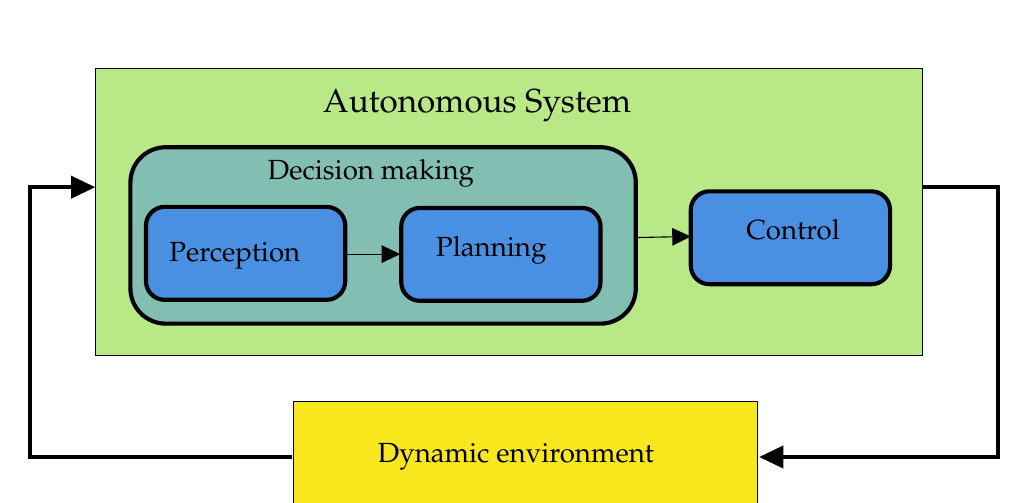
\begin{tikzpicture}[x=0.75pt,y=0.75pt,yscale=-1,xscale=1]
	%uncomment if require: \path (0,300); %set diagram left start at 0, and has height of 300
	
	%Shape: Rectangle [id:dp27957619560066704] 
	\draw  [fill={rgb, 255:red, 184; green, 233; blue, 134 }  ,fill opacity=1 ] (43,48.75) -- (441.5,48.75) -- (441.5,187.25) -- (43,187.25) -- cycle ;
	%Rounded Rect [id:dp7625981193027371] 
	\draw  [color={rgb, 255:red, 0; green, 0; blue, 0 }  ,draw opacity=1 ][fill={rgb, 255:red, 74; green, 144; blue, 226 }  ,fill opacity=1 ][line width=1.5]  (330,116.95) .. controls (330,112.01) and (334.01,108) .. (338.95,108) -- (417.05,108) .. controls (421.99,108) and (426,112.01) .. (426,116.95) -- (426,143.8) .. controls (426,148.74) and (421.99,152.75) .. (417.05,152.75) -- (338.95,152.75) .. controls (334.01,152.75) and (330,148.74) .. (330,143.8) -- cycle ;
	%Straight Lines [id:da826125804046745] 
	\draw    (304.5,130.25) -- (327,129.81) ;
	\draw [shift={(330,129.75)}, rotate = 178.88] [fill={rgb, 255:red, 0; green, 0; blue, 0 }  ][line width=0.08]  [draw opacity=0] (8.93,-4.29) -- (0,0) -- (8.93,4.29) -- cycle    ;
	%Rounded Rect [id:dp7912077043288683] 
	\draw  [color={rgb, 255:red, 0; green, 0; blue, 0 }  ,draw opacity=1 ][fill={rgb, 255:red, 74; green, 144; blue, 226 }  ,fill opacity=0.48 ][line width=1.5]  (60,103.75) .. controls (60,94.36) and (67.61,86.75) .. (77,86.75) -- (286.5,86.75) .. controls (295.89,86.75) and (303.5,94.36) .. (303.5,103.75) -- (303.5,154.75) .. controls (303.5,164.14) and (295.89,171.75) .. (286.5,171.75) -- (77,171.75) .. controls (67.61,171.75) and (60,164.14) .. (60,154.75) -- cycle ;
	%Rounded Rect [id:dp050693216378291606] 
	\draw  [color={rgb, 255:red, 0; green, 0; blue, 0 }  ,draw opacity=1 ][fill={rgb, 255:red, 74; green, 144; blue, 226 }  ,fill opacity=1 ][line width=1.5]  (67.5,124.45) .. controls (67.5,119.51) and (71.51,115.5) .. (76.45,115.5) -- (154.55,115.5) .. controls (159.49,115.5) and (163.5,119.51) .. (163.5,124.45) -- (163.5,151.3) .. controls (163.5,156.24) and (159.49,160.25) .. (154.55,160.25) -- (76.45,160.25) .. controls (71.51,160.25) and (67.5,156.24) .. (67.5,151.3) -- cycle ;
	%Rounded Rect [id:dp6167247502432494] 
	\draw  [color={rgb, 255:red, 0; green, 0; blue, 0 }  ,draw opacity=1 ][fill={rgb, 255:red, 74; green, 144; blue, 226 }  ,fill opacity=1 ][line width=1.5]  (190.5,124.95) .. controls (190.5,120.01) and (194.51,116) .. (199.45,116) -- (277.55,116) .. controls (282.49,116) and (286.5,120.01) .. (286.5,124.95) -- (286.5,151.8) .. controls (286.5,156.74) and (282.49,160.75) .. (277.55,160.75) -- (199.45,160.75) .. controls (194.51,160.75) and (190.5,156.74) .. (190.5,151.8) -- cycle ;
	%Straight Lines [id:da3281578111728798] 
	\draw    (163.5,138.25) -- (179.5,138.25) -- (187,138.25) ;
	\draw [shift={(190,138.25)}, rotate = 180] [fill={rgb, 255:red, 0; green, 0; blue, 0 }  ][line width=0.08]  [draw opacity=0] (8.93,-4.29) -- (0,0) -- (8.93,4.29) -- cycle    ;
	%Shape: Rectangle [id:dp8888738733811714] 
	\draw  [fill={rgb, 255:red, 248; green, 231; blue, 28 }  ,fill opacity=1 ] (138.5,209.25) -- (362,209.25) -- (362,263.75) -- (138.5,263.75) -- cycle ;
	
	%Straight Lines [id:da14809135342937618] 
	\draw [line width=1.5]    (442,106) -- (478,106) -- (478,236) -- (367,236) ;
	\draw [shift={(363,236)}, rotate = 360] [fill={rgb, 255:red, 0; green, 0; blue, 0 }  ][line width=0.08]  [draw opacity=0] (11.61,-5.58) -- (0,0) -- (11.61,5.58) -- cycle    ;
	%Straight Lines [id:da5537882213887542] 
	\draw [line width=1.5]    (138,236) -- (11.5,236) -- (11.5,106) -- (39,106) ;
	\draw [shift={(43,106)}, rotate = 180] [fill={rgb, 255:red, 0; green, 0; blue, 0 }  ][line width=0.08]  [draw opacity=0] (11.61,-5.58) -- (0,0) -- (11.61,5.58) -- cycle    ;
	
	% Text Node
	\draw (151.5,57.5) node [anchor=north west][inner sep=0.75pt]   [align=left] {{\large Autonomous System}};
	% Text Node
	\draw (77.5,131) node [anchor=north west][inner sep=0.75pt]   [align=left] {Perception};
	% Text Node
	\draw (206,128.5) node [anchor=north west][inner sep=0.75pt]   [align=left] {Planning};
	% Text Node
	\draw (355.5,120) node [anchor=north west][inner sep=0.75pt]   [align=left] {Control};
	% Text Node
	\draw (125,91.5) node [anchor=north west][inner sep=0.75pt]   [align=left] {Decision making};
	% Text Node
	\draw (178,228) node [anchor=north west][inner sep=0.75pt]   [align=left] {Dynamic environment};
	
	
\end{tikzpicture}
	\caption{Framework Autonomous System.}
	\label{fig:as_arch}
\end{figure}



 write it in a formal language without iusing complex words, and maintining the same number of words and concept try to uniform this text to be more readable and compact:
Perception, a fundamental aspect of \gls{av} technology, encompasses the intricate interplay between the vehicle's sensory inputs and its understanding of the surrounding environment. Through a symphony of proprioceptive, external, and exteroceptive sensors, \glspl{av} engage in a continuous dialogue with the world around them, shaping their perception of the road ahead. This perceptual framework, characterized by a diverse array of sensor technologies such as radar, cameras, LiDAR, and GPS, forms the bedrock upon which \glspl{av} navigate their operational landscapes.

The choice of sensors is a pivotal decision, with each type offering unique insights into the environment. Cameras, for instance, provide high-resolution visual data, capturing intricate details of the surroundings and facilitating robust object recognition. Radar, on the other hand, excels in detecting objects even in adverse weather conditions, offering a complementary perspective to visual data. LiDAR enhances spatial awareness, mapping out the environment with precision through laser-based technology. GPS, though not a direct sensory input, provides invaluable geospatial context, aiding in localization and route planning.

Yet, beyond the technical intricacies lies the crux of perception: how the \gls{av} interprets and synthesizes these disparate streams of sensor data into a cohesive understanding of its surroundings. Perception, in this context, is not merely the passive reception of sensory inputs but rather an active process of sense-making and contextualization. It involves discerning meaningful patterns from the sensor data, anticipating dynamic changes in the environment, and making informed decisions in real-time.

The perception systems of \glspl{av}, therefore, serve as the eyes and ears of these autonomous entities, shaping their interaction with the world and influencing their behavior on the road. It is through the lens of perception that \glspl{av} navigate complex urban environments, negotiate challenging road conditions, and ensure the safety of passengers and pedestrians alike. As technology advances and perception algorithms grow increasingly sophisticated, the future holds the promise of even greater perceptual acuity for \gls{av}, ushering in an era of safer, more efficient transportation systems.

The planning phase, as a pivotal component of the \gls{av} decision-making continuum, orchestrates a seamless transition from perception to action, synthesizing environmental cues into a cohesive course of action. At its core, this phase encapsulates a sophisticated interplay between machine intelligence and real-world dynamics, where \glspl{av} dynamically chart their trajectory amidst the ever-evolving landscape of their operational milieu.

Within this realm, the AV embarks on a deliberative journey, intricately weaving together inputs garnered from the perception phase with mission objectives and situational imperatives. Whether navigating bustling city streets, traversing expansive highways, or negotiating intricate railway networks, the \gls{av}'s planning algorithm meticulously tailors its trajectory to align with operational exigencies and safety constraints.

Moreover, the adaptability and agility inherent in the planning process imbue \glspl{av} with the capacity to respond nimbly to emergent scenarios, deftly recalibrating their path in real-time to circumvent obstacles and optimize efficiency. This dynamic recalibration, informed by a fusion of sensory inputs and predictive analytics, ensures that the AV remains resilient in the face of uncertainty, fostering a symbiotic relationship between perception and action.

It is imperative to underscore that the nuances of planning are not universal but rather bespoke to the unique characteristics of each AV archetype. Whether terrestrial, aerial, or rail-bound, the planning paradigm undergoes bespoke tailoring to harmonize with the intrinsic attributes and operational exigencies of the vehicle in question. This bespoke tailoring ensures that the planning process remains attuned to the idiosyncrasies of each domain, optimizing performance and fostering seamless integration within the broader transportation ecosystem.

In essence, the planning phase serves as the linchpin of AV autonomy, catalyzing the translation of perception into purposeful action. By orchestrating a symphony of cognitive processes and environmental awareness, this phase not only steers \glspl{av} towards their destination but also paves the way for a future where intelligent transportation systems harmoniously coalesce with the fabric of urban mobility.


Decision-making for autonomous systems involves processes through which these entities make safe and efficient decisions based on environmental information and the state of the system itself. In contexts of autonomous systems, such as \glspl{av}, decision-making is critical for safe navigation and interaction with other road users. This decision-making process encompasses a multitude of factors, including real-time sensor data, predictive analytics, and adherence to predefined rules and regulations.

Classical decision-making methods, such as rule-based systems, optimization algorithms, and probabilistic models, provide a structured approach to handling various scenarios encountered by autonomous systems. Rule-based systems rely on a set of predefined rules to guide decision-making, while optimization algorithms aim to find the best possible solution to a given problem, considering constraints and objectives. Probabilistic models, on the other hand, use statistical inference to estimate the likelihood of different outcomes, enabling decision-making under uncertainty.

In contrast, learning-based methods leverage artificial intelligence techniques to improve decision-making capabilities over time. By learning from large volumes of example data, these methods can adapt and evolve to handle complex and dynamic environments more effectively. Statistical learning techniques, such as support vector machines and decision trees, analyze patterns in data to make predictions or classifications. Deep learning algorithms, which involve neural networks with multiple layers, excel at processing complex sensory inputs, such as images or speech, to make high-level decisions. Reinforcement learning, inspired by behavioral psychology, enables autonomous systems to learn through trial and error, optimizing decisions based on feedback from the environment.

These decision-making methods play a crucial role in enabling autonomous systems to operate autonomously and safely in diverse and unpredictable environments. By combining classical and learning-based approaches, autonomous systems can navigate complex scenarios, anticipate potential hazards, and interact seamlessly with their surroundings, ultimately enhancing safety and efficiency on the road.

Within the domain of \glspl{av}, the control sub-system assumes a critical role in the precise execution of planned trajectories. Its primary function is to guide the vehicle along designated paths as determined by the planning sub-system.

A control system is tasked with regulating or maintaining process conditions within a plant to align with desired values. This is achieved by adjusting certain process variables to manipulate the variables of interest, typically the output variables. In the context of \glspl{av}, the control system is responsible for generating commands for throttle, brake, and steering inputs, which are essential for directing the vehicle's motion parameters such as position, orientation, velocity, acceleration, and jerk.

It's important to clarify that the designation of input and output variables—often referred to as manipulated/process variables and controlled variables, respectively—is with respect to the plant rather than the controller itself, a distinction that can sometimes cause confusion.

The control system plays a pivotal role within the architecture of an autonomous vehicle. As the final component of the pipeline, it assumes the responsibility for physically maneuvering the vehicle. It is the control sub-system that ultimately dictates the behavior of the ego vehicle and its interactions with the surrounding environment.

While the control sub-system relies on inputs from the perception and planning sub-systems, it is equally valid to assert that the latter two are rendered ineffective if the controller fails to accurately track the prescribed trajectory. Thus, the control sub-system not only complements but also completes the holistic framework of AV operation, ensuring seamless navigation and interaction within dynamic environments.



  
\subsection{Future Trends}

The future trends and directions of \glspl{av} are shaped by key insights from global expert discussions. The emphasis is on regulatory frameworks acting as catalysts for \gls{av} deployment, with a focus on safety, environmental impact, and societal benefits. Innovations in freight and public transport systems, such as drone delivery services and autonomous buses, are highlighted. Challenges like congestion, parking, and urban planning are acknowledged, with strategies for addressing these through technological advancements and policy adjustments. The development of common standards and data sharing protocols is vital for global adoption, alongside advancements in cybersecurity to protect emerging AV ecosystems. Overall, the future of \glspl{av} presents a complex interplay of technology, regulation, and societal acceptance, driving towards enhanced safety, efficiency, and environmental sustainability.







\part{PERCEPTION}
\label{part:1}
\lhead{\bfseries PERCEPTION}


\section*{Literature review}

Lane detection remains a cornerstone within the realm of advanced driver assistance systems, representing a critical element for intelligent autonomous systems and applications in smart vehicles. Notably, Lane Departure Warning Systems (LDWS) emerge as indispensable safety mechanisms, serving to alert drivers when their vehicles deviate from designated lanes on highways~\cite{choi2016advanced}. Over recent years, lane detection methodologies have undergone extensive scrutiny, leading to a classification of current studies into three primary categories: feature-based methods~\cite{suddamalla2015novel},~\cite{sehestedt2007robust},~\cite{liu2013lane}, model-based approaches ~\cite{wang2010model},~\cite{wang2004lane}, and deep learning techniques~\cite{kim2014robust},~\cite{zou2019robust}.

Feature-based methodologies typically entail the recognition of lanes through the analysis of lane marking attributes such as color and line edges. In this case, the input images are normally processed with contrast enhancement and edge detection techniques; after that, the lane markings in the image can be detected using a thresholding method, HT~\cite{albanesi1991time} or its variants (i.e., Randomized HT~\cite{mongkonyong2018lane}). However, a notable drawback of feature-based methods lies in their dependency on clearly delineated lane marks, rendering them susceptible to disruptions such as weak lane markings and occlusions. To address these limitations, the concept of Inverse Projection Mapping (IPM) has been introduced~\cite{Borkar2012}. By generating a bird's-eye view of the road surface, IPM circumvents issues associated with obscured or faint lane markings, although its efficacy relies heavily on the assumption of a perfectly flat road surface and precise camera calibration.

In model-based methods, lane markings are identified through the modeling of lanes using predetermined models such as straight-line, parabolic, or spline models. Various algorithms have been proposed, including combinations of Dynamic Programming (DP) and Hough Transform~\cite{wang2010model}, as well as curve model fitting methods in conjunction with gradient enhancement and edge detection techniques~\cite{Yoo2013}. However, the complexity of developing reliable models poses a significant challenge for model-based approaches.

Deep learning techniques, on the other hand, leverage deep learning algorithms, particularly Artificial Neural Networks (ANNs), to extract lane information. These methods, exemplified by the integration of Convolutional Neural Networks (CNNs) with algorithms like RANdom SAmple Consensus (RANSAC)~\cite{kim2014robust} or Recurrent Neural Networks (RNNs)~\cite{zou2019robust}, demonstrate promising capabilities in noise reduction and robust lane detection, especially in scenarios with challenging conditions such as bad lane markings or vehicle occlusion.

Despite their efficacy, the aforementioned state-of-the-art methods often entail high computational demands, particularly deep learning approaches. In response, this work proposes a novel Lane Detection algorithm based on Iterative Tree Search (ITS), designed specifically for low-cost hardware deployment. Characterized by its speed, computational efficiency, and low power consumption, the ITS-based approach represents a significant contribution to the field, offering a promising alternative to existing methodologies. Notably, to the best of our knowledge, there are no other algorithms for lane detection based on Iterative Tree Search, further highlighting the novelty and potential impact of this research endeavor.


Path following constitutes a significant application challenge within the domain of Unmanned Aerial Vehicles (UAVs), holding particular relevance in precision agriculture settings where robust path following algorithms are essential for maintaining high productivity rates and facilitating optimal plant growth~\cite{1_basso2019uav}. Moreover, in civilian applications such as power line monitoring, path following encapsulates the essential task of navigating between multiple target regions requiring inspection~\cite{Silano2021ICRARAL}. Irrespective of the specific application domain, the successful completion of missions by drones hinges upon their ability to safely and accurately follow predefined paths.

Examining the path following problem reveals two distinct components: path detection and path following~\cite{Dahroug2018MARSS, Rafique2020TAES}. In terms of path detection, the Hough transform and its advancements are widely regarded as prominent solutions in the literature s~\cite{6_duan2010improved, Du2010TIMP,5_duda1972use}. However, the computational demands associated with such transformations pose challenges, particularly for on-board implementation in aircraft with stringent battery and processing constraints. These challenges are further exacerbated in the context of Micro Aerial Vehicles (MAVs) where both sensor equipment and vehicle dimensions are minimal. Conversely, lightweight machine learning solutions have emerged as promising alternatives for path detection, albeit the time required for algorithm setup impedes their practical application in real-world scenarios~\cite{7_van2019ls, Tang2021PR}. Hence, there is a growing interest in low computational intensity algorithms capable of providing path following references within predefined time constraints, even without prior knowledge of the surrounding environment.

Transitioning to the path following stage, much of the state-of-the-art solutions~\cite{8_sujit2013evaluation, 12_pelizer2017comparison} rely on the use of nonlinear guidance laws~\cite{Keshmiri2018ICUAS}, vector fields~\cite{Tuttle2021ARC}, and pure pursuit algorithms owing to their simplicity and ease of implementation~\cite{Baqir2020IOP}. While the choice of path planner is contingent upon specific application requirements, certain general considerations can be made. Nonlinear guidance laws, while simple to implement, exhibit degraded performance in scenarios characterized by rapid changes in target acceleration, leading to significant trajectory generation delays and instability~\cite{Keshmiri2018ICUAS}. Consequently, ensuring stability necessitates a comprehensive understanding of target velocity and acceleration dynamics. Conversely, while vector field solutions mitigate oscillation issues inherent in nonlinear guidance laws, they entail substantial computational overhead which is not suitable for embedded systems present on a UAV~\cite{Tuttle2021ARC}. Meanwhile, the pure pursuit approach offers a viable solution for scenarios where tracking accuracy and computational efficiency are paramount. By dynamically adjusting the position of a look-ahead point based on predefined tracking criteria, pure pursuit algorithms aim to minimize the distance between the current position and the anticipated path, thereby facilitating precise path following~\cite{Gautam2015ICUAS, 10_xavier2019path, Silano2019SMC}.



\chapter{Enhanced Vision-Based UAV Path Following Strategy}
\label{Chapter:1}


In this chapter, we embark on an exploration of a novel algorithm designed for unmanned aerial vehicles (UAVs), focusing particularly on the path following and landing accuracy challenges that are pivotal in autonomous flight operations. The emergence of UAVs has revolutionized numerous sectors, including surveillance, delivery services, and environmental monitoring, by offering unprecedented flexibility and access to remote areas. However, the full potential of UAVs is contingent upon the advancement of robust navigation and control algorithms that can ensure precise maneuvering and operational reliability in diverse environments.

This research delves into the development and validation of an innovative algorithm that synergizes the pure pursuit path tracking methodology with advanced image processing techniques. This integration is tailored to enhance path detection and adherence capabilities, enabling UAVs to navigate and complete missions with heightened accuracy and efficiency. The motivation behind this algorithm springs from the need to address the computational constraints of micro aerial vehicles (MAVs), which necessitate lightweight yet effective solutions for real-time path following and target landing tasks.

The chapter sets the stage by outlining the theoretical underpinnings of the pure pursuit algorithm and its adaptation to the unique dynamics of UAV flight. It further discusses the incorporation of image processing for dynamic path detection, a critical component for ensuring the UAV's adaptability to varying operational scenarios. The mathematical models and simulation frameworks employed to evaluate the algorithm's performance are introduced, providing a foundation for the subsequent analysis of numerical results.

A significant highlight of this research is its practical validation through participation in the IFAC2020 MathWorks Minidrone competition, a prestigious event that challenges participants to demonstrate the efficacy of their control algorithms in real-world scenarios. This competition not only serves as a rigorous testing ground for the algorithm but also as a benchmark for its success against international standards.

By offering an open-source implementation of the algorithm, this chapter contributes to the broader UAV research community, facilitating further exploration, adaptation, and enhancement of path following techniques. The introduction sets the tone for a detailed investigation into the algorithm's development, its operational merits, and its triumphant validation in a competitive arena, underscoring its potential to redefine UAV navigation and control paradigms.

\newpage




\section{Problem Description}
\label{sec:problemDescription}

The work presented here finds an application within the IFAC2020 MathWorks Minidrone competition~\cite{4_Mathworks_url}, where the use of a model-based design approach is the aim of the specific contest. Path error and mission time are used as evaluation metrics for the algorithm. The whole process is the following: a quad-rotor~\gls{UAV} follows a pre-established red path by using its downward facing camera to get feedback from the environment. Images are updated according to the position and orientation of the vehicle simulated in the MATLAB~\gls{VR} world. No prior knowledge on the path and the surrounding scenario is given. The drone takes off and starts its motion looking at the path, and the mission stops with the recognition of an end-marker. At that time, the drone lands staying within the delimited area. Figure~\ref{fig:arena} shows the considered scenario. 
%
\begin{figure}[h]
	\centering
	\begin{tikzpicture}
		\node[anchor=south west,inner sep=0] (img) at (0,0) { 
			\includegraphics[width=0.45\textwidth]{figure/Part1/Chapter3/figures/track.png}};
		\begin{scope}[x={(img.south east)},y={(img.north west)}]
			
			% Solid circles for the drones, from left to right
			\draw [white, dashed, ultra thick] (0.95, 0.48) circle (0.065);
			
		\end{scope}
	\end{tikzpicture}
	\caption{Snapshot extracted from the virtual scenario. A dashed circle is used to indicated the drone position.}
	\label{fig:arena}
\end{figure}

\section{Vision-Based Path Following Algorithm}
\label{sec:purPursuitTrackingAlgorithm}


The vision-based path following algorithm combines the advantages offered by the pure pursuit algorithm~\cite{14_coulter1992implementation} with that of an easy image processing system to cope with the task. The algorithm starts selecting a target position ahead of the vehicle and that has to be reached, typically on a path. The framework is based on the following operations: (i) given the actual position $\mathbf{d}=(x_d, y_d)^\top \in \mathbb{R}^2$ where the~\gls{UAV} is located, a~\gls{VTP} is set over the track at $\mathbf{w}=(x_w, y_w)^\top \in \mathbb{R}^2$; then, (ii) the quad-rotor is commanded to reach the~\gls{VTP} along a straight line (essentially it is the pure pursuit algorithm with a curvature of infinite radius)~\cite{14_coulter1992implementation}, i.e., moving the vehicle from its current position to the goal position\footnote{The quad-rotor is assumed to fly at a fixed height along the entire mission.}. In Figure~\ref{fig:pure pursuit} an illustrative example of how the algorithm works is depicted. 

\begin{figure}
	\centering
	\includegraphics[scale=0.75]{figure/Part1/Chapter3/figures/purepursuit.png}
	\caption{An illustrative example of the proposed vision-based path following algorithm works. The red point $\mathbf{d}$ represents the drone position, while the orange point $\mathbf{w}$ depicts the~\gls{VTP}.}
	\label{fig:pure pursuit}
\end{figure}

Contrary to the pure pursuit algorithm, the proposed approach exploits the intrinsic characteristics of the multi-rotor~\glspl{UAV} motion: differently from ground vehicles with steering wheels, drones can follow a path without modifying their heading. Such an assumption allows reducing the time to accomplish the task by removing the control of the heading from the purposes of the path follower. %The testing of the algorithm is performed inside a Simulink virtual scenario, where a path is created as shown in Figure~\ref{fig:arena}. 

In Figure~\ref{fig:block diagram} the whole control scheme architecture is reported. The algorithm is mainly divided into two parts: (i) the~\gls{IPS} deals with extracting the red path from the camera images, providing the errors along the $x$- and $y$-axis of the camera frame between the current drone position and the~\gls{VTP} point, and recognizing the End-Marker for the landing operations; while, (ii) the~\gls{PP} figures out the path following problem by computing the new position $\mathbf{w}$ of the drone in the world frame\cite[Sec.~V]{SilanoMATFly} implementing an~\gls{IBVS} scheme. The control algorithm computes the commands $u_T$, $u_\varphi$, $u_\vartheta$, and $u_\psi$ that should be given to the drone in order to update its position and orientation in accordance to the~\gls{PP} references. 

\begin{figure}
	\begin{center}
		\scalebox{1.2}{
			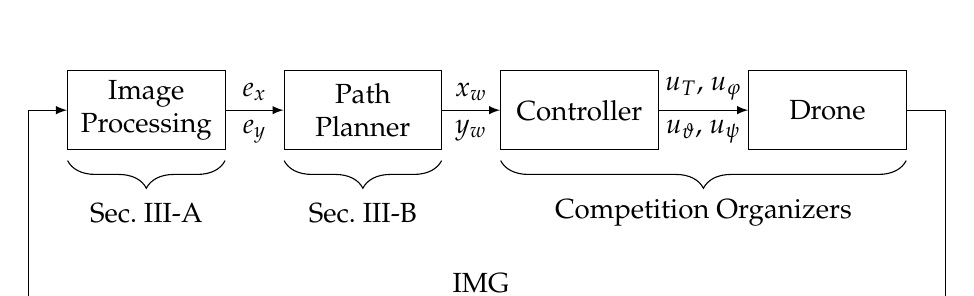
\begin{tikzpicture}
				
				%%%%%%%%%%%%%%%%% Node - Image Processing System
				\node (ImageProcessingSystem) at (-1.5,0) [draw, rectangle, minimum width=2cm, minimum 
				height=1cm, text centered, text width=5em]{Image Processing};
				
				% Curly brackets
				\draw [decorate,decoration={brace, mirror, amplitude=10pt,raise=4pt},yshift=0pt] 
				(-2.5,-0.5) -- (-0.5,-0.5) node [black,midway,xshift=0.0cm,yshift=-0.8cm] {Sec.~III-A};
				
				%%%%%%%%%%%%%%%%% Node - Path Planner
				\node (PathPlanner) at (1.25,0) [draw, rectangle, minimum width=2cm, minimum 
				height=1cm, text centered, text width=5em]{Path Planner};
				
				% Curly brackets
				\draw [decorate,decoration={brace, mirror, amplitude=10pt,raise=4pt},yshift=0pt] 
				(0.25,-0.5) -- (2.25,-0.5) node [black,midway,xshift=0.0cm,yshift=-0.8cm] {Sec.~III-B};
				
				%%%%%%%%%%%%%%%%% Node - Controller
				\node (Controller) at (4.00,0) [draw, rectangle, minimum width=2cm, minimum height=1cm, 
				text centered, text width=5em]{Controller};
				
				%%%%%%%%%%%%%%%%% Node - Drone
				\node (Drone) at (7.15,0) [draw, rectangle, minimum width=2cm, minimum height=1cm, text 
				centered, text width=5em]{Drone};
				
				% Curly brackets
				\draw [decorate,decoration={brace, mirror, amplitude=10pt,raise=4pt},yshift=0pt] 
				(3.00,-0.5) -- (8.15,-0.5) node [black,midway,xshift=0.0cm,yshift=-0.8cm] {Competition Organizers};
				
				% Links
				\draw[-latex] (ImageProcessingSystem) -- node[above]{$e_x$} node[below]{$e_y$} (PathPlanner);
				\draw[-latex] (PathPlanner) -- node[above]{$x_w$} node[below]{$y_w$} (Controller);
				\draw[-latex] (Controller) -- node[above]{$u_T$, $u_\varphi$} node[below]{$u_\vartheta$, $u_\psi$} (Drone);
				\draw[-latex] (Drone) -- ($ (Drone) + (1.5,0)$) -- ($ (Drone) + (1.5,-2.5)$) -- ($ 
				(ImageProcessingSystem) - (1.5,2.5)$) -- ($ (ImageProcessingSystem) - (1.5,0)$) --  
				(ImageProcessingSystem);
				
				% Text
				\node at ($ (PathPlanner) - (-1.5,2.45)$) [text centered, above]{IMG};
				
			\end{tikzpicture}
		}
	\end{center}
	\caption{Control system architecture. From left to right: the image processing, path planner, controller, and drone blocks.}
	\label{fig:block diagram}
\end{figure}

The overall mission is divided into four parts: \textit{Take off}, \textit{Following}, \textit{End-Marker}, and \textit{Landing}. A decision-making process has been implemented to achieve the competition objectives triggering the system from a state to another, as depicted in Figure~\ref{fig:state machine}. For each frame, the~\gls{IPS} accesses the system status and plan the next action (i.e., landing, following, etc.). The drone starts taking off from its initial position looking at the path. Once the vehicle reaches the hovering position, the~\gls{IPS} detects the path and the state machine enters in the \textit{Following} state, hence the path following starts. As soon as the~\gls{IPS} detects the End-Marker, the state machine exits from the \textit{Following} state and goes into the \textit{End-Marker} state. At this stage the mission stops, and the drone starts the landing. In the following subsections the implementation of the image processing system and path planner modules are detailed.
%
\begin{figure}
	\centering
	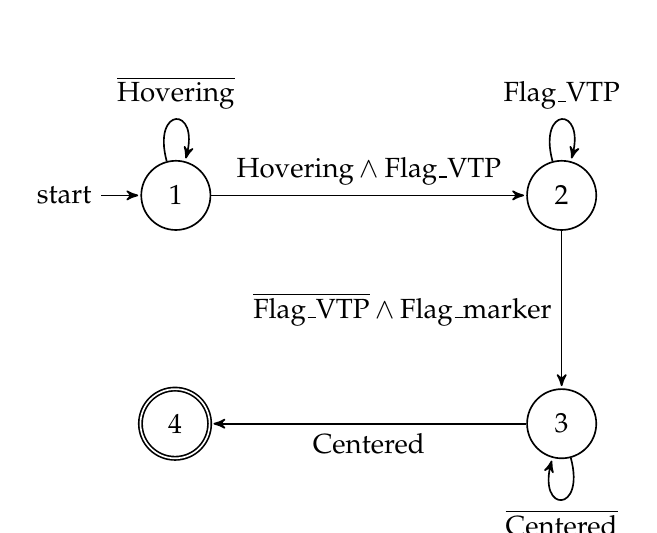
\begin{tikzpicture}[->, >=stealth', shorten >=0.8pt, auto, semithick, initial text=${\rm start}$]
		
		\tikzstyle{every state}=[fill=white,text=black]
		
		\node[initial,state] (A)                    {$1$};
		\node[state]         (B)        [ right= 4cm of A] {$2$};
		\node[state]         (C) [ below= 2cm of B] {$3$};
		\node[accepting,state](D) [ left= 4cm of C] {$4$};
		
		\path (A) edge              node {${ \rm Hovering} \wedge {\rm Flag\_VTP}$} (B)
		edge [loop above] node {{${ \rm \overline{Hovering}}$}} (A)
		(B) edge       [left]       node {${ \rm \overline{Flag\_VTP} \wedge Flag\_marker}$} (C)
		edge [loop above] node {${ \rm Flag\_VTP}$} (B)
		(C) edge              node {${\rm Centered}$} (D)
		edge [loop below] node {${ \rm \overline{Centered}}$} (C);
		
	\end{tikzpicture}
	\caption{State machine implemented. State 1: \textit{Take-off}. State 2: \textit{Following}. State 
		3: \textit{End-Marker}. State 4: \textit{Landing}.} 
	\label{fig:state machine}
\end{figure} 


\subsection{Image processing system}
\label{sec:imageProcessingSystem}

Starting from the camera frames, the~\gls{IPS} takes care of separating the features of the pre-established path from that of the environment. % The main objective of the module is in the detection, especially track  and landing mark detection in the \textit{Track} and \textit{End-Marker} phases, respectively. Moreover, the~\ac{IPS} is in charge of triggering the state machine from a state to another and to handle the decision-making process during the competition mission.

The~\gls{IPS} receives frames of width $W$ and height $H$ from the camera sensor at each   $T_\mathrm{IPS} = \SI{0.2}{\second}$, i.e., the camera sampling time. The image format is RGB with $8$ bits for each color channel. The path is \SI{0.01}{\meter} in width, while the landing marker is circular with a diameter of \SI{0.02}{\meter}. The path color is red, and this information is taken into consideration in all the elaborations to filter out the background scenario. The procedure consists of the following steps: first, the RGB frame is converted into an intensity level frame representation as follows 
%
\begin{equation}
	F(n,m)=f_R(n,m) -  \frac{f_G(n,m)}{GG} - \frac{f_B(n,m)}{GB} ,
\end{equation}
%
where the pair $(n,m)$ represents the pixel located at row $n \in \{1, 2, \dots, H\}$ and column $m \in \{1, 2, \dots, W\}$ of the image frame and $f_i$, with $i \in \{R, G, B\}$, provides the intensity level representation of the corresponding red, green and blue channels. An heuristic approach was used to tune the $GG$, $GB \geq 1$ parameter values. These parameters help to detect the pixels belonging to the path. Further, a binarization process based on a $K_T$  threshold value refines the process removing artifacts from the elaboration. The binarized frame can be described by the binary function $F_\mathrm{bin} \colon (n,m) \to \{0, 1\}$ whose output is one when the pixel belongs to the path and zero otherwise. Finally, an erosion operation is performed through a square kernel to shrink and regularize the binarized frame. In Figure~\ref{fig:preprocessing} the overall process is reported for a single sample frame.

\begin{figure}
	\centering
	\includegraphics[width=0.75\textwidth]{figure/Part1/Chapter3/figures/bin_ero_track.jpg}
	\caption{Original frame (upper left),  converted and binarized frame (upper right), and eroded frame (lower).}
	\label{fig:preprocessing}
\end{figure}

Then, the obtained reference path is used in a twofold way: (i) to identify a new~\gls{VTP} belonging to the track; (ii) to detect the landing marker. The two tasks are described in the pseudocode reported in Algorithm~\ref{alg:imageProcessing}.

Looking at the algorithm, the first three functions (i.e., \texttt{channelConv}, \texttt{binarization}, and \texttt{erosion}) take care of extracting the path information from the frame. Then, the \texttt{detectTrack} and \texttt{detectMarker} functions deal with raising a flag when the path (\texttt{Flag\_VTP}) or the End-Marker (\texttt{Flag\_marker}) are detected. The path following algorithm starts with the~\gls{IPS} that computes the errors ($e_x$ and $e_y$) between the drone position and the~\gls{VTP} point for the~\gls{PP} by using a circular arc mask centered in the drone~\gls{CoM}\footnote{The assumption that the~\gls{CoM} being in the center of the reference frame, i.e., $x_\mathrm{CoM} = \frac{H}{2}$ and $y_\mathrm{CoM}=\frac{W}{2}$, is taken into consideration.} with thickness $R_\mathrm{max} - R_\mathrm{min}$\footnote{$R_\mathrm{max}$ and $R_\mathrm{min}$ are the outer and inner radius, respectively.}. 
%
% FOR ALGORITHM UAV
\def\BState{\State\hskip-\ALG@thistlm}
%
\begin{algorithm}
	\caption{Image Processing System}\label{alg:imageProcessing}
	\begin{algorithmic}[1]
		\State $\text{IMG}  \gets \text{channelConv(\text{IMG})}$, \\
		$\text{IMG} \gets \text{binarization(\text{IMG})}$, \\
		$\text{IMG} \gets \text{erosion(\text{IMG})}$, \\
		$\text{Flag\_VTP} \gets \text{detectTrack(\text{IMG})}$, \\
		$\text{Flag\_marker}$ $\gets \text{detectMarker(\text{IMG})}$
		
		\If {$\text{Flag\_VTP}$} \\ 
		\quad $x_\mathrm{VTP}$, $y_\mathrm{VTP} \gets \text{vtp(frame)}$ \\
		\quad $e_x \gets x_\mathrm{VTP} - x_\mathrm{CoM}$ \\
		\quad $e_y \gets y_\mathrm{VTP} - y_\mathrm{CoM}$
		\Else \If{$\text{Flag\_marker}$} \\
		\quad \quad $\;$ $x_\mathrm{MARK}$, $y_\mathrm{MARK} \gets \text{cgMarker(frame)}$ \\
		\quad \quad $\;$ $e_x \gets x_\mathrm{MARK} - x_\mathrm{CoM}$ \\ 
		\quad \quad $\;$ $e_y \gets y_{\rm MARK} - y_{\rm CoM}$
		\EndIf \EndIf
		
		\State \Return $e_x$, $e_y$, $\text{Flag\_VTP}, \text{Flag\_marker}$ 
	\end{algorithmic}
\end{algorithm}


In Figure~\ref{fig:Arc_mask}, the arc mask considering the~\gls{VTP} position at time $\mathbf{t}_k$ is depicted, where $\mathbf{t}_k$ denotes the $k$-element of the time interval vector defined as $\mathbf{t} =(0, T_\mathrm{IPS}, \dots, NT_\mathrm{IPS})^\top \in \mathbb{R}^{N+1}$, with $k \in \mathbb{N}_0$. The orientation angle \mbox{$\vartheta = \arctantwo(x_\mathrm{VTP},y_\mathrm{VTP})$} is calculated with respect to the frame coordinates, where the $\arctantwo$ function is the four-quadrant inverse of the tangent function. A portion~$\varTheta$ of the arc mask is established by taking into account the previous~\gls{VTP}'s orientation. In particular, we set up two semi-arcs with width~$\frac{\varTheta}{2}$, namely~\gls{FOV}, in counter-clockwise and clockwise directions from $\vartheta$. Then, the arc mask is applied to the eroded image obtaining the~\gls{VTP} point at $\mathbf{t}_{k+1}$. The function~\gls{VTP} calculates $x_\mathrm{VTP}$, $y_\mathrm{VTP}$, and $\vartheta$ which represent the frame coordinates and angle orientation of the~\gls{VTP} at  $\mathbf{t}_{k+1}$, respectively. Subsequently the corresponding errors with respect to the center of mass, i.e., $e_x$ and $e_y$, are computed inside the frame coordinates. Finally, the \texttt{Flag\_VTP} and the $e_x$ and $e_y$ values are provided as input to the~\gls{PP} at each $T_\mathrm{IPS}$. Figure~\ref{fig:track} shows the result of the entire process setup. 

\begin{figure}
	\begin{center}
		\scalebox{1.65}{
			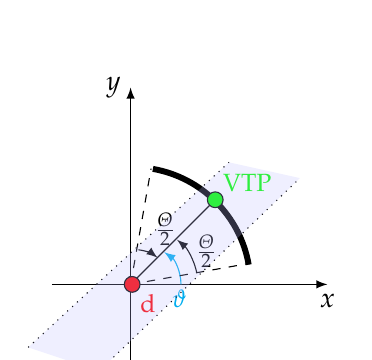
\begin{tikzpicture}
				
				% Axes of the image frame
				\draw[-latex] (-1.00,0) -- (2.5,0) node[below]{$x$};
				\draw[-latex] (0,-1.0) -- (0,2.5) node[left]{$y$};
				
				% Circle of the circular mask
				\draw[line width=2.15pt] (1.5,0.25) arc(10:80:1.5);
				
				% Radius
				\draw[-] (0,0) -- (1.05,1.05);
				%\node at (0.75,0.75) [left]{\scriptsize $R_\mathrm{min}$};
				%\node at (1.25,1.45) [left]{\scriptsize $R_\mathrm{max}$};
				
				% Length errors
				%\draw[green,-, line width=1.25pt] (0,0) -- node[above left]{\small $e_y$} (0,1.04);
				%\draw[blue,-, line width=1.25pt] (0,0) -- node[below right]{\small $e_x$} (1,0);
				%\draw[dotted] (1,0) -- (1,1.04);
				%\draw[dotted] (0,1.04) -- (1,1.04);
				\draw (0,0) arc(0:20:0.3);
				\draw[-latex] (0.84,0.15) arc (12:50:0.75cm);
				\node at (0.70,0.75) [below right]{\small $\frac{\varTheta}{2}$}; % first angle
				\draw[-latex] (0.10,0.44) arc (82.5:52:0.5cm);
				\node at (0.70,0.70) [left]{\small $\frac{\varTheta}{2}$}; % second angle
				\draw[-latex, cyan] (0.64,0) arc (0:55:0.5cm);
				\node at (0.40,0.05) [below right, cyan]{\small $\vartheta$}; % first angle
				
				% End
				\draw[dashed] (0,0) -- (0.26,1.47); % cos(80)*1.5, sin(80)*1.5
				\draw[dashed] (0,0) -- (1.47,0.26); % cos(10)*1.5, sin(10)*1.5
				\draw[fill=red] (-0.08,0) arc(-180:180:0.1); % balls
				\node at (0,0) [below right]{\textcolor{red}{\small{d}}};
				\draw[fill=green] (0.975,1.075) arc(-180:180:0.1); % balls
				\draw (1.05, 1.05) node[above right]{\textcolor{green}{\small{VTP}}};
				
				% Adding path
				\draw[dotted] (-1.30, -0.80) -- (1.25,1.55);
				\draw[dotted] (-0.40, -1.10) -- (2.15,1.35);
				\fill[blue!25, nearly transparent] (-1.30, -0.80) -- (1.25,1.55) -- (2.15,1.35) -- 
				(-0.40, -1.10) -- cycle;
				
			\end{tikzpicture}
		}
	\end{center}
	\caption{Arc mask. The drone position (red), the previous~\gls{VTP} (green), and the pre-established path to follow (purple) are reported.} 
	\label{fig:Arc_mask}
\end{figure}
%
\begin{figure}
	\centering
	\includegraphics[width=0.75\textwidth]{figure/Part1/Chapter3/figures/VTP_Algorithm_1.png}
	\caption{Frame after the application of the Arc mask (left). Extracted pixels belonging to the path (right).}
	\label{fig:track}
\end{figure}

It is worth noticing that when the landing marker is detected and no other~\gls{VTP} point is found in the frame, the~\gls{IPS} triggers the state machine in the \texttt{End-Marker} state. Here, the new main task of the~\gls{IPS} is to obtain the position of the End-Marker within the frame coordinates. An additional erosion process is performed by using a circular kernel, as depicted in Figure~\ref{fig:End_marker}. 

\begin{figure}
	\centering
	\includegraphics[width=0.75\textwidth]{figure/Part1/Chapter3/figures/land_marker.png}
	\caption{Original (left) and eroded frames (right) of the End-Marker are reported.}
	\label{fig:End_marker}
\end{figure}

\subsection{Path planner}
\label{sec:pathPlanner}

The~\gls{PP} is designed to compute the position of the~\gls{VTP} point $\mathbf{w} = (x_w, y_w)^\top$ maintaining a constant altitude ($z_H$) while following the path. Roughly speaking, the~\gls{PP} computes the spatial coordinates $x_w$ and $y_w$ trying to reduce the errors, i.e., $e_x$ and $e_y$, between the drone position and the~\gls{VTP}. These values are later used by the drone controller to tune the command signals $u_T$, $u_\varphi$, $u_\vartheta$, and $u_\psi$, as described in Figure~\ref{fig:block diagram}. The proposed path planner is based on~\gls{PI} control loops. As a common rule in cascade structure, the inner loop, i.e., the~\gls{PP}, is regulated at a rate faster than the outer loop, i.e., the~\gls{IPS}. In our case, the~\gls{PP} runs at $\SI{200}{\hertz}$ ($T_\mathrm{PP} = \num{5e-3} \si{\second}$) while the~\gls{IPS} runs at $\SI{2}{\hertz}$ ($T_\mathrm{IPS} = \SI{0.2}{\second}$). These are a standard solution in the literature for quad-rotors control design~\cite{Dief2015}.

As described in Sec.~\ref{sec:purPursuitTrackingAlgorithm}, the path following stops with the detection of the End-Marker. At that time, the~\gls{IPS} implements a toggle switch behavior raising the \texttt{Flag\_marker} flag while holding low the \texttt{Flag\_VTP} flag. This mutually separates the \textit{Following} and \textit{Landing} phases avoiding instability issues. The pseudocode of the proposed algorithm is reported in Algorithm~\ref{alg:pathPlanner} with parameter values detailed in Table~\ref{tab:parameters}.

In Subsection~\ref{subsec:uavVelocity}, we show how $\alpha$ can be set to control the velocity of vehicle along the entire mission. Therefore, the proposed Vision-Based Path Following algorithm makes it possible not only to generate the spatial coordinates $x_w$ and $y_w$ using a~\gls{IBVS} scheme but also to set the velocity during the entire mission.

\begin{algorithm}
	\caption{Path Planner}\label{alg:pathPlanner}
	\begin{algorithmic}[1]
		\State $e_x$, $e_y$, $\text{Flag\_VTP}$, $\text{Flag\_marker}$ 
		
		\If{$\text{Flag\_VTP}$} \\
		\quad $x_{k+1} \gets x_k + \alpha e_x$\\
		\quad $y_{k+1} \gets y_k + \alpha e_y$\\
		\quad $z_{k+1} \gets  z_H$
		\EndIf
		
		\If{$\text{Flag\_marker}$}
		\If{$(e_x=0 \wedge e_y=0)$} \\
		\quad \quad $\;$ $x_{k+1}  \gets x_k $\\
		\quad \quad $\;$ $y_{k+1} \gets y_k $\\
		\quad \quad $\;$ $z_{k+1} \gets 0$
		\Else \\
		\quad \quad $\;$ $x_{k+1} \gets x_k + \beta e_x$\\
		\quad \quad $\;$ $y_{k+1}  \gets y_k + \beta e_y$\\
		\quad \quad $\;$ $z_{k+1} \gets z_H$
		\EndIf \EndIf
		
		\State $x_w \gets x_{k+1}$, $y_w \gets y_{k+1}$, $z_w \gets z_{k+1}$
		
		\State \Return $x_w$, $y_w$, $z_w$
	\end{algorithmic}
\end{algorithm} 

%The~\ac{PP} obtains the state position estimations every \mbox{$T_\mathrm{PP}=\SI{0.05}{\second}$}; consequently, it can plan a new position to reach according to its sampling time. The behavior of the PP depends on the state machine, there are two operating modes: one is implemented to track a~\ac{VTP} and the other one is employed to reach the central point of the End-Marker. The two dynamic behaviors differ from each other: the~\ac{PP} used to track a~\ac{VTP} has to produce a trajectory with a high velocity and a minimum error between the~\ac{CG} of the drone and the arena track. The control parameter $\alpha$ regulates the operating mode during the \textit{Track} phase, choosing high values allow to decrease the time to reach the~\ac{VTP}. During the \textit{End-Marker}, the drone has to reach the End-Marker position with a good accuracy avoiding to overtake it, for this reason the values of the control parameters $\beta$, which regulates this drone behavior during this phase, have to be low.

%%% END SECTION ============================================================

%%% START SECTION ==========================================================

\section{Numerical Results}
\label{sec:simulationsResults}

To demonstrate the validity and effectiveness of the proposed framework, numerical simulations have been carried out by using the 2019b release of MATLAB equipped with MathWorks Virtual Reality toolbox~\cite{16_Mathworks_url} and Parrot support package for Simulink~\cite{15_Mathworks_url}. The video available at~\cite{YouTubeVideo} illustrates in a direct way how the system works, i.e., the ability of the quad-rotor~\gls{UAV} to follow the pre-established red path and to land on the End-Marker. In addition, the video shows the behavior of the~\gls{IPS} and~\gls{PP} that never lose the path during the entire mission. 
%The testing of the algorithm is performed inside a Simulink virtual scenario, where a path is created as shown in Figure~\ref{fig:arena}. 

In Figure~\ref{fig:plot_trajectory} a comparison of the system performance by using various values of $\alpha$ is reported. As can be seen from the plots, the larger $\alpha$ is, the lower the mission time ($T_s$) is. On the other hand, the lower the mission time is, the greater the path error is. Looking at the zoom plot (see, Figure~\ref{subfig:comparisonPlot}) it is even clearer how the system performance degrades with increasing $\alpha$ value, and these are all the more evident as the path is angular. For the considered scenario, an heuristic approach was used to tune the $\alpha$ and $\beta$ parameter values.



\begin{figure}[t]
	\begin{center}
		\hspace{-0.725cm}
		\begin{subfigure}[c]{0.45\columnwidth}
			\scalebox{0.8}{
				\begin{tikzpicture}
					\begin{axis}[%
						width=2.8119in,%
						height=1.8183in,%
						at={(0.758in,0.481in)},%
						scale only axis,%
						xmin=-3.7,%
						xmax=0,%
						ymax=3,%
						ymin=-0.25,%
						xmajorgrids,%
						ymajorgrids,%
						ylabel style={yshift=0cm}, %shifting the y line text
						xlabel={X [\si{\meter}]},%
						ylabel={Y [\si{\meter}]},%
						axis background/.style={fill=white},%
						legend style={at={(0.725,0.875)},anchor=north,legend cell align=left, draw=none, 
							draw=white!15!black}
						]
						%
						\addplot [color=blue, solid, line width=1.15pt] 
						file{figure/Part1/Chapter3/matlabPlots/track_downsampled.txt};%
						%
						\addplot [color=red, dashed, line width=1.15pt] 
						file{figure/Part1/Chapter3/matlabPlots/alpha_005_downsampled.txt};%
						%
						\legend{$\text{path}$, $\alpha = 0.05\text{,}\, T_s = \SI{30}{\second}$};%
					\end{axis}
				\end{tikzpicture}
			}
			\caption{}
		\end{subfigure}
		%
		\hspace{0.25cm}
		%
		\begin{subfigure}[c]{0.45\columnwidth}
			\scalebox{0.8}{
				\begin{tikzpicture}
					\begin{axis}[%
						width=2.8119in,%
						height=1.8183in,%
						at={(0.758in,0.481in)},%
						scale only axis,%
						xmin=-3.7,%
						xmax=0,%
						ymax=3,%
						ymin=-0.25,%
						xmajorgrids,%
						ymajorgrids,%
						ylabel style={yshift=0cm}, %shifting the y line text
						xlabel={X [\si{\meter}]},%
						ylabel={Y [\si{\meter}]},%
						axis background/.style={fill=white},%
						legend style={at={(0.725,0.875)},anchor=north, legend cell align=left, draw=none, 
							draw=white!15!black}
						]
						%
						\addplot [color=blue, solid, line width=1.15pt] 
						file{figure/Part1/Chapter3/matlabPlots/track_downsampled.txt};%
						%
						\addplot [color=green, dashed, line width=1.15pt] 
						file{figure/Part1/Chapter3/matlabPlots/alpha_004_downsampled.txt};%
						%
						\legend{$\text{path}$, $\alpha = 0.04\text{,}\, T_s = \SI{34}{\second}$};%
					\end{axis}
				\end{tikzpicture}
			}
			\caption{}
		\end{subfigure}
		%
		\\
		\vspace{0.05cm}
		\hspace{-0.75cm}
		%
		\begin{subfigure}[c]{0.45\columnwidth}
			\scalebox{0.8}{
				\begin{tikzpicture}
					\begin{axis}[%
						width=2.8119in,%
						height=1.8183in,%
						at={(0.758in,0.481in)},%
						scale only axis,%
						xmin=-3.7,%
						xmax=0,%
						ymax=3,%
						ymin=-0.25,%
						xmajorgrids,%
						ymajorgrids,%
						ylabel style={yshift=0cm}, %shifting the y line text
						xlabel={X [\si{\meter}]},%
						ylabel={Y [\si{\meter}]},%
						axis background/.style={fill=white},%
						legend style={at={(0.725,0.875)},anchor=north,legend cell align=left, draw=none, draw=white!15!black}
						]
						%
						\addplot [color=blue, solid, line width=1.15pt] 
						file{figure/Part1/Chapter3/matlabPlots/track_downsampled.txt};%
						%
						\addplot [color=yellow, dashed, line width=1.15pt] 
						file{figure/Part1/Chapter3/matlabPlots/alpha_003_downsampled.txt};%
						%
						\legend{$\text{path}$, $\alpha = 0.03\text{,}\, T_s = \SI{47}{\second}$};%
					\end{axis}
				\end{tikzpicture}
			}
			\caption{}
		\end{subfigure}
		%
		\hspace{0.25cm}
		%
		\begin{subfigure}[c]{0.45\columnwidth}
			\scalebox{0.8}{
				\begin{tikzpicture}
					\begin{axis}[%
						width=2.8119in,%
						height=1.8183in,%
						at={(0.758in,0.481in)},%
						scale only axis,%
						xmin=-3.7,%
						xmax=-3.4,%
						ymax=3,%
						ymin=2,%
						xmajorgrids,%
						ymajorgrids,%
						ylabel style={yshift=0cm}, %shifting the y line text
						xlabel={X [\si{\meter}]},%
						ylabel={Y [\si{\meter}]},%
						axis background/.style={fill=white},%
						legend style={at={(0.475,0.945)},anchor=north,legend cell align=left, draw=none, legend columns=-1, draw=white!15!black}
						]
						%
						\addplot [color=red, dashed, line width=1.15pt] 
						file{figure/Part1/Chapter3/matlabPlots/alpha_005_downsampled.txt};%
						%
						\addplot [color=green, dashed, line width=1.15pt] 
						file{figure/Part1/Chapter3/matlabPlots/alpha_004_downsampled.txt};%
						%
						\addplot [color=yellow, dashed, line width=1.15pt] 
						file{figure/Part1/Chapter3/matlabPlots/alpha_003_downsampled.txt};%
						%
						\legend{$\alpha = 0.05$, $\alpha = 0.04$, $\alpha = 0.03$};%
						%
						\addplot [color=blue, solid, line width=1.15pt] 
						file{figure/Part1/Chapter3/matlabPlots/track_downsampled.txt};%
						%
					\end{axis}
				\end{tikzpicture}
			}
			\caption{}
			\label{subfig:comparisonPlot}
		\end{subfigure}
	\end{center}
	\caption{Trajectory plots. From left to right: the desired and the drone paths for various values of $\alpha$ are represented. The mission time $T_s$ and a comparison between the considered $\alpha$ values are also reported.}
	\label{fig:plot_trajectory}
\end{figure}

%\begin{figure}
%	\begin{center}
	%		\scalebox{1}{
		%			\begin{tikzpicture}
			%			\begin{axis}[%
				%			width=2.8119in,%
				%			height=1.8183in,%
				%			at={(0.758in,0.481in)},%
				%			scale only axis,%
				%			xmin=-3.7,%
				%			xmax=0,%
				%			ymax=3,%
				%			ymin=-0.25,%
				%			xmajorgrids,%
				%			ymajorgrids,%
				%			ylabel style={yshift=0cm}, %shifting the y line text
				%			xlabel={X [\si{\meter}]},%
				%			ylabel={Y [\si{\meter}]},%
				%			axis background/.style={fill=white},%
				%			legend style={at={(0.725,0.875)},anchor=north,legend cell 
					%				align=left,draw=none,draw=white!15!black}
				%			]
				%			%
				%			\addplot [color=blue, solid, line width=1.15pt] 
				%			file{matlabPlots/track_downsampled.txt};%
				%			%
				%			\addplot [color=red, dotted, line width=1.15pt, mark size=2, mark repeat=3, 
				%			mark=diamond*] file{matlabPlots/alpha_003_downsampled.txt};%
				%			%
				%			\addplot [color=green, dotted, line width=1.15pt, mark=x, mark size=2, mark repeat=3] 
				%			file{matlabPlots/alpha_004_downsampled.txt};%
				%			%
				%			\addplot [color=magenta, dotted, line width=1.15pt, mark=o, mark size=1, mark 
				%			repeat=3] file{matlabPlots/alpha_005_downsampled.txt};%
				%			%
				%			\legend{$\text{track}$, $\alpha = 0.03\text{,}\, T_s = \SI{47}{\second}$, $\alpha = 
					%			0.04\text{,}\, T_s = \SI{34}{\second}$, $\alpha = 0.05\text{,}\, T_s = 
					%			\SI{30}{\second}$};%
				%			\end{axis}
			%			\end{tikzpicture}
		%		}
	%	\end{center}
%	\caption{Trajectory plot. The desired and the drone paths for various $\alpha$ are represented. 
	%	The mission time $T_s$ is also reported.}
%	\label{fig:plot_trajectory}
%\end{figure}

Figure~\ref{fig:plot_velocity} depicts the drone velocity $v_x$ and $v_y$ along the $x$- and $y$-axis, respectively, and the norm of the drone velocity $v_D$. As described in Sec.~\ref{sec:pathPlanner} and detailed in~\ref{subsec:uavVelocity}, the norm of the drone velocity remains approximately constant while following the path. The presence of spikes might be due to the coupling effects of the drone $xy$ dynamics even though $x_w$ and $y_w$ references have not been modified yet (see, Figure~\ref{fig:plot_trajectory}). Such coupling effects are probably caused by the asymmetric positioning of the rotors with respect to the principal axis and the effect of the discrete image pixelization. 
%
\begin{figure}
	\begin{center}
		\scalebox{1.1}{
			\begin{tikzpicture}
				\begin{axis}[%
					width=2.8119in,%
					height=1.4183in,%
					at={(0.758in,0.481in)},%
					scale only axis,%
					xmin=0,%
					xmax=35,%
					ymax=0.5,%
					ymin=-0.5,%
					xmajorgrids,%
					ymajorgrids,%
					ylabel style={yshift=0cm}, %shifting the y line text
					xlabel={Time [\si{\second}]},%
					ylabel={Velocity [\si{\meter\per\second}]},%
					axis background/.style={fill=white},%
					legend style={at={(0.425,0.175)},anchor=north,legend cell 
						align=left,draw=none,legend columns=-1,align=left,draw=white!15!black}
					]
					%
					\addplot [color=blue, dotted, line width=1.15pt] 
					file{figure/Part1/Chapter3/matlabPlots/vd_downsampled.txt};%
					%
					\addplot [color=red, dashed, line width=1.15pt] 
					file{figure/Part1/Chapter3/matlabPlots/vy_downsampled.txt};%
					%
					\addplot [color=green, solid, line width=1.15pt] 
					file{figure/Part1/Chapter3/matlabPlots/vx_downsampled.txt};%
					%
					\legend{$v_D$, $v_y$, $v_x$};%
				\end{axis}
			\end{tikzpicture}
		}
	\end{center}
	\caption{Velocity plot.}
	\label{fig:plot_velocity}
\end{figure}

\subsection{UAV Velocity Control}
\label{subsec:uavVelocity}

Let us consider a continuous-time dynamical system $\pazocal{H}$ and its discrete time version $x_{k+1}=f(x_k,u_k)$, where $x_k, x_{k+1} \in X \subset \mathbb{R}^n$ are the current state and the next state of the system, respectively, $u \in U \subset \mathbb{R}^m$ is the control input. Let us consider the~\gls{PP} algorithm implementation detailed in Algorithm~\ref{alg:pathPlanner}. Hence, the next state of the system $x_{k+1}$ and $y_{k+1}$ along the $x$- and $y$-axis can be written as follows:
%
\begin{equation}
	x_{k+1} = x_k + \alpha e_{x_k}, \qquad y_{k+1} = y_k + \alpha e_{y_k},
\end{equation}
%
respectively. After some simple algebra, we can write:
%
\begin{equation}
	\dfrac{x_{k+1}-x_k}{T_{\rm PP}} = \dfrac{\alpha e_{x_k}}{T_{\rm PP}}, \qquad 
	%
	\dfrac{y_{k+1}-y_k}{T_{\rm PP}} = \dfrac{\alpha e_{y_k}}{T_{\rm PP}}, 
\end{equation}
%
and hence,
%
\begin{equation}
	v_x \approx \dfrac{\alpha e_{x_k}}{T_{\rm PP}} = \tilde{\alpha} e_{x_k}, \qquad 
	%
	v_y  \approx  \dfrac{\alpha e_{y_k}}{T_{\rm PP}} = \tilde{\alpha} e_{y_k},
\end{equation}
%
with $\tilde{\alpha} = \frac{\alpha}{T_{\rm PP}}$.

Knowing that $e_{x_k}$ and $e_{y_k}$ are by definition the projections over a circle along the $x$- and $y$-axis of the~\gls{VTP} with an angle $\vartheta_k$, we can write
%
\begin{equation}
	\begin{array}{rll}
		e_{x_k} &=& \dfrac{R_\mathrm{max}+R_\mathrm{min}}{2} \sin{\vartheta_k},\\[10pt]
		e_{y_k} &=& \dfrac{R_\mathrm{max}+R_\mathrm{min}}{2} \cos{\vartheta_k},
	\end{array}
\end{equation}
%
and thus,
%
\begin{equation} 
	\begin{split}
		V_D & = \sqrt{v_x^2 + v_y^2} \approx \tilde{\alpha} \dfrac{R_\mathrm{max}+R_\mathrm{min}}{2}. \\
	\end{split}
\end{equation}
%
Hence the parameter $\alpha$ controls the drone velocity. 






\newpage
\section{Chapter Summary}


The chapter provides a comprehensive analysis of a novel winner-prize algorithm designed for path following in UAVs, specifically within the context of the IFAC2020 MathWorks Minidrone competition. This algorithm integrates the pure pursuit algorithm with simple image processing for path detection and tracking, optimized for deployment on MAVs with limited computational capacity. Through MATLAB simulations and the MathWorks VR toolbox, the effectiveness of this approach is validated, emphasizing its practical applicability and open-source availability for replication and further study.

The numerical results section highlights the algorithm's performance through various simulations, demonstrating its capability to efficiently follow a prior established path and accurately land on an end-marker. Adjustments in the algorithm's parameters, such as $\alpha$, show a trade-off between mission time and path error, providing insights into its adaptability and tuning for specific mission requirements. The velocity analysis further underscores the system's robustness, maintaining consistent velocity while managing the dynamics and discrete pixelization effects inherent in UAV operations.

This chapter culminates in affirming the algorithm's significance, not only through its empirical success in simulations but also by winning a prestigious competition. This accolade serves as a testament to its innovative design, operational efficiency, and potential impact on future UAV path following and autonomous navigation research. The open-source availability of the code further enhances its contribution to the field, encouraging ongoing development and application in various UAV operations.




\chapter{An Iterative Approach for Real-Time Lane Detection}
\label{Chapter:2}

\newacronym{ADAS}{ADAS}{Advanced Driver Assistance System}
\newacronym{LWDS}{LWDS}{Lane Departure Warning Systems}
\newacronym{ITS}{ITS}{Iterative Tree Search}
\newacronym{ROI}{ROI}{Region Of Interest}
\newacronym{RGB}{RGB}{Red Green Blue}
\newacronym{RP}{RP}{Root Pixel}
\newacronym{CP}{CP}{Child Pixel}
\newacronym{HT}{HT}{Hough Transform}

In this chapter, we introduce an innovative lane detection approach utilizing an Iterative Tree Search (ITS) algorithm, tailored for real-time application in autonomous driving systems. Amidst the growing need for advanced driver-assistance systems (ADAS) and the evolution of autonomous vehicles, lane detection remains a critical challenge, demanding high accuracy and computational efficiency. The ITS algorithm, by operating directly at the pixel level without relying on traditional feature extraction methods or complex mathematical modeling, presents a novel solution that is both resource-efficient and adaptable to various driving conditions.

Our focus is on demonstrating the algorithm's superior performance, particularly in environments with fluctuating illumination and diverse road conditions. The methodology's uniqueness lies in its lower computational complexity, making it ideal for implementation on less powerful hardware platforms without compromising the detection accuracy or operational speed. This approach not only showcases the potential for significant advancements in real-time lane detection but also opens avenues for its integration into low-cost, low-power embedded systems, paving the way for broader applications in the automotive industry.

The experimental setup, detailed herein, leverages real-world driving scenarios to evaluate the algorithm's effectiveness across different lighting conditions, illustrating its robustness and reliability. Through comparative analysis with state-of-the-art algorithms, we highlight the ITS algorithm's competitive edge in performance, underscoring its feasibility for enhancing road safety and the autonomy of driving systems. This chapter sets the stage for a comprehensive discussion on the development, implementation, and validation of this groundbreaking lane detection algorithm, aiming to contribute significantly to the fields of autonomous driving and machine perception.

\newpage

\section{Proposed Method}
\label{sec:proposed_algorithm}
The proposed method consists of three main phases: frame acquisition, image preprocessing and~\gls{ITS}, as shown in Fig.~\ref{fig:Scheme}.
\noindent Images from the highway environment are acquired through a front-facing camera directed towards the road, the image preprocessing block reports the steps employed to enhance the image features by eliminating unwanted falsification, while the~\gls{ITS} block is the core of the novel lane detection approach proposed in this work.

\begin{figure}[ht]
	\centering
	
\centering


\tikzset{every picture/.style={line width=0.75pt}} %set default line width to 0.75pt        

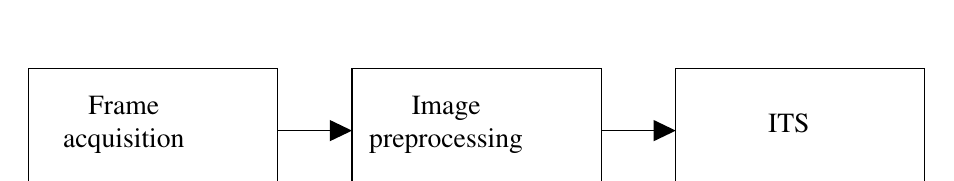
\begin{tikzpicture}[x=0.75pt,y=0.75pt,yscale=-1.2,xscale=1.2]
%uncomment if require: \path (0,300); %set diagram left start at 0, and has height of 300

%Shape: Rectangle [id:dp5311967622096787] 
\draw  [fill={rgb, 255:red, 255; green, 255; blue, 255 }  ,fill opacity=1 ] (20,20) -- (120,20) -- (120,70) -- (20,70) -- cycle ;
%Shape: Rectangle [id:dp07593828947048697] 
\draw  [fill={rgb, 255:red, 255; green, 255; blue, 255 }  ,fill opacity=1 ] (150,20) -- (250,20) -- (250,70) -- (150,70) -- cycle ;
%Shape: Rectangle [id:dp1321828393456428] 
\draw  [fill={rgb, 255:red, 255; green, 255; blue, 255 }  ,fill opacity=1 ] (280,20) -- (380,20) -- (380,70) -- (280,70) -- cycle ;
%Straight Lines [id:da24611526462953326] 
\draw    (120,45) -- (147,45) ;
\draw [shift={(150,45)}, rotate = 180] [fill={rgb, 255:red, 0; green, 0; blue, 0 }  ][line width=0.08]  [draw opacity=0] (8.93,-4.29) -- (0,0) -- (8.93,4.29) -- cycle    ;
%Straight Lines [id:da283033721708871] 
\draw    (250,45) -- (277,45) ;
\draw [shift={(280,45)}, rotate = 180] [fill={rgb, 255:red, 0; green, 0; blue, 0 }  ][line width=0.08]  [draw opacity=0] (8.93,-4.29) -- (0,0) -- (8.93,4.29) -- cycle    ;

% Text Node
\draw (30.67,30.00) node [anchor=north west][inner sep=0.75pt]   [align=left] {\begin{minipage}[lt]{48.000000pt}\setlength\topsep{0pt}
\begin{center}
{\fontfamily{ptm}\selectfont Frame}\\{\fontfamily{ptm}\selectfont  acquisition}
\end{center}

\end{minipage}};
% Text Node
\draw (152,30) node [anchor=north west][inner sep=0.75pt]   [align=left] {\begin{minipage}[lt]{62.482752pt}\setlength\topsep{0pt}
\begin{center}
{\fontfamily{ptm}\selectfont Image}\\{\fontfamily{ptm}\selectfont  preprocessing}
\end{center}

\end{minipage}};
% Text Node
\draw (316,37) node [anchor=north west][inner sep=0.75pt]   [align=left] {{\fontfamily{ptm}\selectfont ITS}};


\end{tikzpicture}

	\caption{Flow Diagram of the proposed method.}
	\label{fig:Scheme}
\end{figure}


The following assumptions are made for the lane detection problem: the lane boundary lines are made of a light color, (e.g., white or yellow); the road has only an ego-lane and lane boundary lines are not covered from other traffic participants. In the following, the three phases reported in Fig.~\ref{fig:Scheme} will be discussed in detail.




\subsection{Frame acquisition}
\label{subsec:Frame_acquisition}


The camera sensor sends~\gls{RGB} format frames to the embedded system. Let $F_i \in \mathbb{R}^{m \times n}$ be the acquired frame channel, where $m\times n$ is the frame size and $i \in \{r,g,b\}$ represent the red, green and blue channel, respectively.

In Figure \ref{fig:road_original} a frame captured from the road scene is presented.

%
\begin{figure}[ht]
	\centering
	\includegraphics[scale=0.55]{figure/Part1/Chapter4/figures/way2.png}
	\caption{Original frame captured from the highway environment.}
	\label{fig:road_original}
\end{figure}

\begin{figure}[ht]
	\centering
	\includegraphics[scale=0.45]{figure/Part1/Chapter4/figures/way3.png}
	\caption{Grayscale conversion and median filtering.}
	\label{fig:road_original_grey}
\end{figure}



\subsection{Image Preprocessing}
\label{subsec:IP}

Usually, an image taken from the highway scenario includes objects that are not significant for lane detection purposes (e.g., trees, clouds, parts of sky, car hood) and these irrelevant objects decrease the overall performance of the algorithm, so in order to clean the original frame from unnecessary information, this image preprocessing step is mandatory. The first step of the image preprocessing consist of a conversion from~\gls{RGB} color model to intensity level frame. Intensity-level conversion is performed by the
weighted sum of~\gls{RGB} frame as follows~\cite{rgbtogray}:
%
\begin{equation}
	I(u,v)=w_r F_r(u,v) + w_g F_g(u,v) + w_b F_b(u,v),
\end{equation}
%
where  $u \in \big\{1, \dots, m\big\}$ and $v \in \big\{1,\dots,n \big\}$ represent the row and column of the selected pixel and $w_r$, $w_g,$ $w_b \in \mathbb{R}$ are the conversion weights of~\gls{RGB} channels. The result of the intensity level conversion can be seen in Figure \ref{fig:road_original_grey}. This conversion reduces the cardinality of the frame and henceforth the computational load placed on the hardware. Furthermore, in order to improve the performances of the lane detection system, a median filter~\cite{gonzalez2002digital} is used, a particular non-linear technique of digital filtering. The application of the filtering stage has two advantages: i) it allows to reduce the noise and ii) it preserves the edges from the captured frame.
Typically, the lane boundary lines are located in the bottom region of a road frame. Taking into account this observation, an isosceles trapezoid~\gls{ROI} operation to restrict the frame information to the road area is performed. Furthermore, shrinking the frame dimensions means that the computational cost of the detection algorithm is further reduced. This procedure is a well known image preprocessing technique as reported in \cite{Kumar2015Stato}. The major base, minor base and the height of the isosceles trapezoid~\gls{ROI} expressed in pixels are $B_{\rm ROI}$, $b_{\rm ROI}$ and $H_{\rm ROI}$, respectively. From now every operation will done on the~\gls{ROI} frame $I_{ \rm ROI} \in \mathbb{R}^{m_{ \rm ROI} \times n_{ \rm ROI}}$, the latter represents an appropriate rectangle matrix where the elements outside the isosceles trapezoid are considered zero.

In Figure~\ref{fig:final_image_preprocessing} the outcome of the image preprocessing  block is shown. 
%
\begin{figure}[ht]
	\centering
	\includegraphics[scale=0.55]{figure/Part1/Chapter4/figures/ROI.png}
	\caption{Frame after the image preprocessing phase. Frame coordinates (Red). Trapezoid major base (Green). Trapezoid minor base (Orange). Trapezoid height (Yellow).}
	\label{fig:final_image_preprocessing}
\end{figure}
%










\subsection{ITS}
\label{subsec:ITS}
The algorithm is in charge to find the pixels belonging to the lane boundary line and is based on an iterative tree search which allows to reduce the lane detection complexity. The concept of this algorithm derives from the idea that the image can be seen as a set of nodes, where these nodes are represented by the pixels. Lane boundaries are solid lines, uniform in color and different from the road color; an edge between the road background and lane boundary lines allows to distinguish the latter from the road in a frame. These structural properties are reformulated from a pixel property point of view.

To explain the~\gls{ITS} algorithm the terms from tree theory are inherited:~\gls{RP} node and~\gls{CP} node. 
%All the above terms have the same meaning of the original tree search theory, but they are applied to the pixel notion. 
In particular, the~\gls{RP} node and~\gls{CP} node contain the intensity level of the pixel. Since the ego-lane has only two lane boundary lines, the algorithm is applied in parallel for each of those.

The first step of the~\gls{ITS} algorithm is to find the first pixel belonging to the lane boundary line, i.e,~\gls{RP}  node. The first~\gls{RP} node is searched among the pixels present in the first row of~\gls{ROI} as reported in Figure~\ref{fig:rootpixel}. Generally, the lane boundary line has a higher intensity level respect to the road; this allows to find the~\gls{RP} node as the pixel having the highest intensity level. In Figure~\ref{fig:rootframe} the intensity level profile regarding the first row of the~\gls{ROI} is shown, where two peaks are distinguishable that represents the two~\gls{RP}  nodes for the two lane boundary lines.

\begin{figure}[ht]
	\centering
	\includegraphics[scale=0.55]{figure/Part1/Chapter4/figures/roi.png}
	\caption{Finding the~\gls{RP} nodes. First pixel row~\gls{ROI} (Red).~\gls{RP} nodes (Blue). }
	\label{fig:rootpixel}
\end{figure}

\begin{figure} [ht]
	\centering
	\includegraphics[scale=0.3]{figure/Part1/Chapter4/figures/plot.png}
	\caption{Intensity level first row~\gls{ROI}.}
	\label{fig:rootframe}
\end{figure} 



Once the first~\gls{RP}  node is found, a number $N_c$ of~\gls{CP}  nodes are inspected to find another pixel belonging to the lane boundary line on the above row of $I_{\rm ROI}$. The choice is based on the following score function $J$ which measures the score obtained from all the~\gls{CP}  nodes:
%
\begin{equation} \label{eq:J}
		J(u,v)= \alpha I_{\rm ROI}(u,v) - \beta \mid v - v_r \mid +
		-\gamma \mid I_{\rm ROI}(u,v)-I_{\rm ROI}(u_r,v_r) \mid,
\end{equation}
%
where $u,v$  $\big(u_r,v_r\big)$ represent the row and column of~\gls{CP} node \mbox{(\gls{RP} node)}, respectively. The parameters $\alpha$, $\beta$ and $\gamma$ are used to weight the contributes coming from the three addends. The first addend is the intensity level of the~\gls{CP} node, the second and third addends are the distance and the color dissimilarity between the~\gls{CP} node and root pixel node, respectively. 
The first term encourage the choice of brighter pixels; the second term penalizes the pixels that are farther from the root pixel, while the third term is added to encourage the uniformity of intensity between the~\gls{RP} and~\gls{CP}.
Once the functional scores are calculated for each~\gls{CP} node, the one with highest score become the new~\gls{RP} node. Finally the pair $\big(u_r, v_r \big)$ is saved into a memory buffer. The algorithm is iterated until the~\gls{RP} node row reaches the height $H_{\rm ROI}$ of the~\gls{ROI}. In Algorithm~\ref{alg:ITSAlg} the entire procedure is reported.

\begin{algorithm}
	\caption{ITS}\label{alg:ITSAlg}
	\begin{algorithmic}[1]
		\State  $u_r \gets 1$
		\State   $v_r \gets \text{FindRoot}(u_r)$
		\State $LaneSet \gets (u_r,v_r) $
		\While{$u_r \leq H_{ \rm ROI}$}
		\For{$v \in \big\{ v_r-\frac{N_c}{2},\dots,v_r+\frac{N_c}{2}\big\} $}
		\State \text{score function in \eqref{eq:J}.}
		\EndFor
		\State $v_r = \argmax_v \; J(u_r,v)$
		\State $LaneSet \gets (u_r,v_r) $
		\State  $u_r \gets u_r +1$
		\EndWhile
		\State \Return $LaneSet$
	\end{algorithmic}
\end{algorithm} 


\noindent A illustration of the proposed algorithm is presented in Figure~\ref{fig:ITS_double}. In  Fig.~\ref{fig:u1} the~\gls{RP} node is represented with the yellow square. This pixel has been chosen as the pixel with the maximum intensity between the ones in the first row of~\gls{ROI}. The green squares represent the~\gls{CP} nodes, and for each one of them, the score function presented in~\eqref{eq:J} is evaluated. Then, the new~\gls{RP} node will be chosen among the~\gls{CP} nodes as the one that maximise the score function (Fig.~\ref{fig:u2}).

\begin{figure}[ht]
	\begin{subfigure}[b]{\textwidth}
		\centering
		


\tikzset{every picture/.style={line width=0.75pt}} %set default line width to 0.75pt        

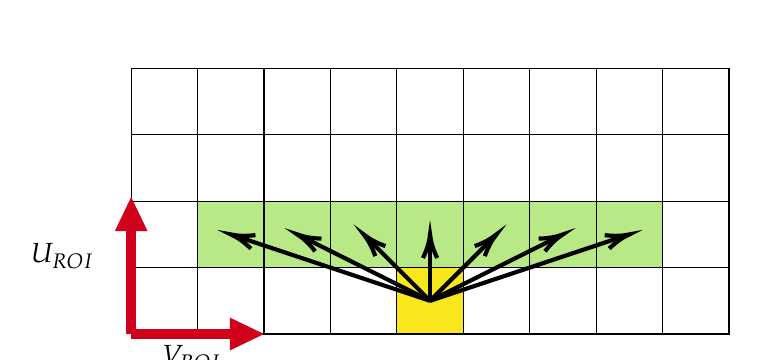
\begin{tikzpicture}[x=0.75pt,y=0.75pt,yscale=-0.8,xscale=0.8]
%uncomment if require: \path (0,300); %set diagram left start at 0, and has height of 300

%Shape: Rectangle [id:dp37479279946268607] 
\draw   (157,53) -- (197,53) -- (197,93) -- (157,93) -- cycle ;
%Shape: Rectangle [id:dp9386900567441059] 
\draw   (197,53) -- (237,53) -- (237,93) -- (197,93) -- cycle ;
%Shape: Rectangle [id:dp40563047766175897] 
\draw   (237,53) -- (277,53) -- (277,93) -- (237,93) -- cycle ;
%Shape: Rectangle [id:dp5068636395583868] 
\draw   (277,53) -- (317,53) -- (317,93) -- (277,93) -- cycle ;
%Shape: Rectangle [id:dp8547935475054569] 
\draw   (317,53) -- (357,53) -- (357,93) -- (317,93) -- cycle ;
%Shape: Rectangle [id:dp7875634623224428] 
\draw   (357,53) -- (397,53) -- (397,93) -- (357,93) -- cycle ;
%Shape: Rectangle [id:dp48004515510156187] 
\draw   (397,53) -- (437,53) -- (437,93) -- (397,93) -- cycle ;
%Shape: Rectangle [id:dp24690344103074247] 
\draw   (477,53) -- (517,53) -- (517,93) -- (477,93) -- cycle ;
%Shape: Rectangle [id:dp92756370861019] 
\draw   (437,53) -- (477,53) -- (477,93) -- (437,93) -- cycle ;
%Shape: Rectangle [id:dp27395603578063277] 
\draw   (157,93) -- (197,93) -- (197,133) -- (157,133) -- cycle ;
%Shape: Rectangle [id:dp1408582450054794] 
\draw   (197,93) -- (237,93) -- (237,133) -- (197,133) -- cycle ;
%Shape: Rectangle [id:dp2887808288270002] 
\draw   (237,93) -- (277,93) -- (277,133) -- (237,133) -- cycle ;
%Shape: Rectangle [id:dp33037939362347357] 
\draw   (277,93) -- (317,93) -- (317,133) -- (277,133) -- cycle ;
%Shape: Rectangle [id:dp3538768626341806] 
\draw   (317,93) -- (357,93) -- (357,133) -- (317,133) -- cycle ;
%Shape: Rectangle [id:dp9814839313159069] 
\draw   (357,93) -- (397,93) -- (397,133) -- (357,133) -- cycle ;
%Shape: Rectangle [id:dp12604922129270824] 
\draw   (397,93) -- (437,93) -- (437,133) -- (397,133) -- cycle ;
%Shape: Rectangle [id:dp3422014175969996] 
\draw   (477,93) -- (517,93) -- (517,133) -- (477,133) -- cycle ;
%Shape: Rectangle [id:dp7920304225353518] 
\draw   (437,93) -- (477,93) -- (477,133) -- (437,133) -- cycle ;
%Shape: Rectangle [id:dp18661999462756818] 
\draw   (157,133) -- (197,133) -- (197,173) -- (157,173) -- cycle ;
%Shape: Rectangle [id:dp18791201855733464] 
\draw  [fill={rgb, 255:red, 184; green, 233; blue, 134 }  ,fill opacity=1 ] (197,133) -- (237,133) -- (237,173) -- (197,173) -- cycle ;
%Shape: Rectangle [id:dp5629889443468381] 
\draw  [fill={rgb, 255:red, 184; green, 233; blue, 134 }  ,fill opacity=1 ] (237,133) -- (277,133) -- (277,173) -- (237,173) -- cycle ;
%Shape: Rectangle [id:dp503276244238676] 
\draw  [fill={rgb, 255:red, 184; green, 233; blue, 134 }  ,fill opacity=1 ] (277,133) -- (317,133) -- (317,173) -- (277,173) -- cycle ;
%Shape: Rectangle [id:dp4070792760484063] 
\draw  [fill={rgb, 255:red, 184; green, 233; blue, 134 }  ,fill opacity=1 ] (317,133) -- (357,133) -- (357,173) -- (317,173) -- cycle ;
%Shape: Rectangle [id:dp2619995679469691] 
\draw  [fill={rgb, 255:red, 184; green, 233; blue, 134 }  ,fill opacity=1 ] (357,133) -- (397,133) -- (397,173) -- (357,173) -- cycle ;
%Shape: Rectangle [id:dp8991355658683184] 
\draw  [fill={rgb, 255:red, 184; green, 233; blue, 134 }  ,fill opacity=1 ] (397,133) -- (437,133) -- (437,173) -- (397,173) -- cycle ;
%Shape: Rectangle [id:dp03123946616100537] 
\draw   (477,133) -- (517,133) -- (517,173) -- (477,173) -- cycle ;
%Shape: Rectangle [id:dp6406090567697098] 
\draw  [fill={rgb, 255:red, 184; green, 233; blue, 134 }  ,fill opacity=1 ] (437,133) -- (477,133) -- (477,173) -- (437,173) -- cycle ;
%Shape: Rectangle [id:dp923072610195202] 
\draw   (157,173) -- (197,173) -- (197,213) -- (157,213) -- cycle ;
%Shape: Rectangle [id:dp40649773535656464] 
\draw   (197,173) -- (237,173) -- (237,213) -- (197,213) -- cycle ;
%Shape: Rectangle [id:dp05637699840141841] 
\draw   (237,173) -- (277,173) -- (277,213) -- (237,213) -- cycle ;
%Shape: Rectangle [id:dp10908609515836498] 
\draw   (277,173) -- (317,173) -- (317,213) -- (277,213) -- cycle ;
%Shape: Rectangle [id:dp1978162709414546] 
\draw  [fill={rgb, 255:red, 248; green, 231; blue, 28 }  ,fill opacity=1 ] (317,173) -- (357,173) -- (357,213) -- (317,213) -- cycle ;
%Shape: Rectangle [id:dp09177043950937769] 
\draw   (357,173) -- (397,173) -- (397,213) -- (357,213) -- cycle ;
%Shape: Rectangle [id:dp840673321356215] 
\draw   (397,173) -- (437,173) -- (437,213) -- (397,213) -- cycle ;
%Shape: Rectangle [id:dp4916817832684255] 
\draw   (477,173) -- (517,173) -- (517,213) -- (477,213) -- cycle ;
%Shape: Rectangle [id:dp73827422693894] 
\draw   (437,173) -- (477,173) -- (477,213) -- (437,213) -- cycle ;
%Straight Lines [id:da8560297776013615] 
\draw [line width=1.5]    (337,193) -- (219.85,153.95) ;
\draw [shift={(217,153)}, rotate = 378.43] [color={rgb, 255:red, 0; green, 0; blue, 0 }  ][line width=1.5]    (14.21,-4.28) .. controls (9.04,-1.82) and (4.3,-0.39) .. (0,0) .. controls (4.3,0.39) and (9.04,1.82) .. (14.21,4.28)   ;
%Straight Lines [id:da27817194509681964] 
\draw [line width=1.5]    (337,193) -- (259.68,154.34) ;
\draw [shift={(257,153)}, rotate = 386.57] [color={rgb, 255:red, 0; green, 0; blue, 0 }  ][line width=1.5]    (14.21,-4.28) .. controls (9.04,-1.82) and (4.3,-0.39) .. (0,0) .. controls (4.3,0.39) and (9.04,1.82) .. (14.21,4.28)   ;
%Straight Lines [id:da07123008278456933] 
\draw [line width=1.5]    (337,193) -- (299.12,155.12) ;
\draw [shift={(297,153)}, rotate = 405] [color={rgb, 255:red, 0; green, 0; blue, 0 }  ][line width=1.5]    (14.21,-4.28) .. controls (9.04,-1.82) and (4.3,-0.39) .. (0,0) .. controls (4.3,0.39) and (9.04,1.82) .. (14.21,4.28)   ;
%Straight Lines [id:da81869629277768] 
\draw [line width=1.5]    (337,193) -- (337,156) ;
\draw [shift={(337,153)}, rotate = 450] [color={rgb, 255:red, 0; green, 0; blue, 0 }  ][line width=1.5]    (14.21,-4.28) .. controls (9.04,-1.82) and (4.3,-0.39) .. (0,0) .. controls (4.3,0.39) and (9.04,1.82) .. (14.21,4.28)   ;
%Straight Lines [id:da7756735099229475] 
\draw [line width=1.5]    (337,193) -- (374.88,155.12) ;
\draw [shift={(377,153)}, rotate = 495] [color={rgb, 255:red, 0; green, 0; blue, 0 }  ][line width=1.5]    (14.21,-4.28) .. controls (9.04,-1.82) and (4.3,-0.39) .. (0,0) .. controls (4.3,0.39) and (9.04,1.82) .. (14.21,4.28)   ;
%Straight Lines [id:da07783001016646374] 
\draw [line width=1.5]    (337,193) -- (414.32,154.34) ;
\draw [shift={(417,153)}, rotate = 513.4300000000001] [color={rgb, 255:red, 0; green, 0; blue, 0 }  ][line width=1.5]    (14.21,-4.28) .. controls (9.04,-1.82) and (4.3,-0.39) .. (0,0) .. controls (4.3,0.39) and (9.04,1.82) .. (14.21,4.28)   ;
%Straight Lines [id:da5414037753227225] 
\draw [line width=1.5]    (337,193) -- (454.15,153.95) ;
\draw [shift={(457,153)}, rotate = 521.5699999999999] [color={rgb, 255:red, 0; green, 0; blue, 0 }  ][line width=1.5]    (14.21,-4.28) .. controls (9.04,-1.82) and (4.3,-0.39) .. (0,0) .. controls (4.3,0.39) and (9.04,1.82) .. (14.21,4.28)   ;
%Straight Lines [id:da8047399591588045] 
\draw [color={rgb, 255:red, 208; green, 2; blue, 27 }  ,draw opacity=1 ][line width=3.75]    (157,213) -- (157,137.5) ;
\draw [shift={(157,130.5)}, rotate = 450] [fill={rgb, 255:red, 208; green, 2; blue, 27 }  ,fill opacity=1 ][line width=0.08]  [draw opacity=0] (20.54,-9.87) -- (0,0) -- (20.54,9.87) -- cycle    ;
%Straight Lines [id:da39334795544652645] 
\draw [color={rgb, 255:red, 208; green, 2; blue, 27 }  ,draw opacity=1 ][line width=3.75]    (157,213) -- (230,213) ;
\draw [shift={(237,213)}, rotate = 180] [fill={rgb, 255:red, 208; green, 2; blue, 27 }  ,fill opacity=1 ][line width=0.08]  [draw opacity=0] (20.54,-9.87) -- (0,0) -- (20.54,9.87) -- cycle    ;

% Text Node
\draw (95,157) node [anchor=north west][inner sep=0.75pt]    {$U_{ROI}$};
% Text Node
\draw (174,218) node [anchor=north west][inner sep=0.75pt]    {$V_{ROI}$};


\end{tikzpicture}

		\caption{}
		\label{fig:u1}
	\end{subfigure}
	\\[3ex]
	\begin{subfigure}[b]{\textwidth}
		\centering
		


\tikzset{every picture/.style={line width=0.75pt}} %set default line width to 0.75pt        

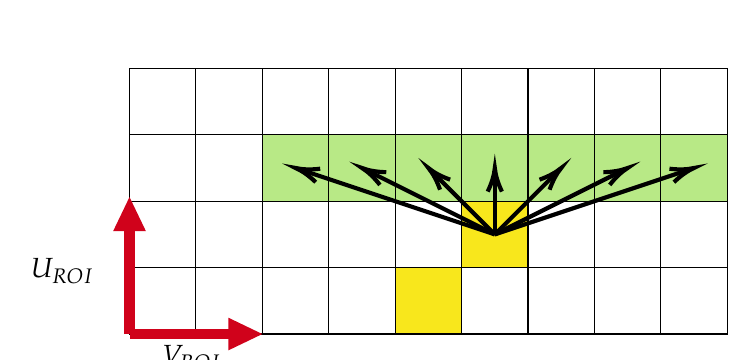
\begin{tikzpicture}[x=0.75pt,y=0.75pt,yscale=-0.8,xscale=0.8]
%uncomment if require: \path (0,300); %set diagram left start at 0, and has height of 300

%Shape: Rectangle [id:dp44188910505312085] 
\draw   (196,145) -- (236,145) -- (236,185) -- (196,185) -- cycle ;
%Shape: Rectangle [id:dp17982965297494968] 
\draw   (236,145) -- (276,145) -- (276,185) -- (236,185) -- cycle ;
%Shape: Rectangle [id:dp22515587821006955] 
\draw   (276,145) -- (316,145) -- (316,185) -- (276,185) -- cycle ;
%Shape: Rectangle [id:dp11801076383471742] 
\draw  [fill={rgb, 255:red, 248; green, 231; blue, 28 }  ,fill opacity=1 ] (316,145) -- (356,145) -- (356,185) -- (316,185) -- cycle ;
%Shape: Rectangle [id:dp9089046489603911] 
\draw   (356,145) -- (396,145) -- (396,185) -- (356,185) -- cycle ;
%Shape: Rectangle [id:dp7896999403341205] 
\draw   (396,145) -- (436,145) -- (436,185) -- (396,185) -- cycle ;
%Shape: Rectangle [id:dp9713409962967257] 
\draw   (436,145) -- (476,145) -- (476,185) -- (436,185) -- cycle ;
%Shape: Rectangle [id:dp014859460901382793] 
\draw   (156,145) -- (196,145) -- (196,185) -- (156,185) -- cycle ;
%Shape: Rectangle [id:dp9620038332096106] 
\draw   (476,145) -- (516,145) -- (516,185) -- (476,185) -- cycle ;
%Shape: Rectangle [id:dp9318475849101779] 
\draw   (196,25) -- (236,25) -- (236,65) -- (196,65) -- cycle ;
%Shape: Rectangle [id:dp23554291041537723] 
\draw   (236,25) -- (276,25) -- (276,65) -- (236,65) -- cycle ;
%Shape: Rectangle [id:dp6788071985488238] 
\draw   (276,25) -- (316,25) -- (316,65) -- (276,65) -- cycle ;
%Shape: Rectangle [id:dp6202713322137914] 
\draw   (316,25) -- (356,25) -- (356,65) -- (316,65) -- cycle ;
%Shape: Rectangle [id:dp771670694696643] 
\draw   (356,25) -- (396,25) -- (396,65) -- (356,65) -- cycle ;
%Shape: Rectangle [id:dp48752893858306945] 
\draw   (396,25) -- (436,25) -- (436,65) -- (396,65) -- cycle ;
%Shape: Rectangle [id:dp8558160524482463] 
\draw   (436,25) -- (476,25) -- (476,65) -- (436,65) -- cycle ;
%Shape: Rectangle [id:dp9591030266017664] 
\draw   (156,25) -- (196,25) -- (196,65) -- (156,65) -- cycle ;
%Shape: Rectangle [id:dp40356174570980485] 
\draw   (476,25) -- (516,25) -- (516,65) -- (476,65) -- cycle ;
%Shape: Rectangle [id:dp47130309531175807] 
\draw   (196,65) -- (236,65) -- (236,105) -- (196,105) -- cycle ;
%Shape: Rectangle [id:dp4748802662239511] 
\draw  [fill={rgb, 255:red, 184; green, 233; blue, 134 }  ,fill opacity=1 ] (236,65) -- (276,65) -- (276,105) -- (236,105) -- cycle ;
%Shape: Rectangle [id:dp11159600208179388] 
\draw  [fill={rgb, 255:red, 184; green, 233; blue, 134 }  ,fill opacity=1 ] (276,65) -- (316,65) -- (316,105) -- (276,105) -- cycle ;
%Shape: Rectangle [id:dp2885743588567362] 
\draw  [fill={rgb, 255:red, 184; green, 233; blue, 134 }  ,fill opacity=1 ] (316,65) -- (356,65) -- (356,105) -- (316,105) -- cycle ;
%Shape: Rectangle [id:dp8432572496496091] 
\draw  [fill={rgb, 255:red, 184; green, 233; blue, 134 }  ,fill opacity=1 ] (356,65) -- (396,65) -- (396,105) -- (356,105) -- cycle ;
%Shape: Rectangle [id:dp8352049942769133] 
\draw  [fill={rgb, 255:red, 184; green, 233; blue, 134 }  ,fill opacity=1 ] (396,65) -- (436,65) -- (436,105) -- (396,105) -- cycle ;
%Shape: Rectangle [id:dp8429572386016915] 
\draw  [fill={rgb, 255:red, 184; green, 233; blue, 134 }  ,fill opacity=1 ] (436,65) -- (476,65) -- (476,105) -- (436,105) -- cycle ;
%Shape: Rectangle [id:dp26640609195013454] 
\draw   (156,65) -- (196,65) -- (196,105) -- (156,105) -- cycle ;
%Shape: Rectangle [id:dp07095927085369014] 
\draw  [fill={rgb, 255:red, 184; green, 233; blue, 134 }  ,fill opacity=1 ] (476,65) -- (516,65) -- (516,105) -- (476,105) -- cycle ;
%Shape: Rectangle [id:dp4884033403677166] 
\draw   (196,105) -- (236,105) -- (236,145) -- (196,145) -- cycle ;
%Shape: Rectangle [id:dp9615981099361754] 
\draw   (236,105) -- (276,105) -- (276,145) -- (236,145) -- cycle ;
%Shape: Rectangle [id:dp7798644660619822] 
\draw   (276,105) -- (316,105) -- (316,145) -- (276,145) -- cycle ;
%Shape: Rectangle [id:dp8219025004188054] 
\draw   (316,105) -- (356,105) -- (356,145) -- (316,145) -- cycle ;
%Shape: Rectangle [id:dp06887054649368096] 
\draw  [fill={rgb, 255:red, 248; green, 231; blue, 28 }  ,fill opacity=1 ] (356,105) -- (396,105) -- (396,145) -- (356,145) -- cycle ;
%Shape: Rectangle [id:dp6604033014043791] 
\draw   (396,105) -- (436,105) -- (436,145) -- (396,145) -- cycle ;
%Shape: Rectangle [id:dp6485467100115199] 
\draw   (436,105) -- (476,105) -- (476,145) -- (436,145) -- cycle ;
%Shape: Rectangle [id:dp8619997043000098] 
\draw   (156,105) -- (196,105) -- (196,145) -- (156,145) -- cycle ;
%Shape: Rectangle [id:dp610853992697381] 
\draw   (476,105) -- (516,105) -- (516,145) -- (476,145) -- cycle ;
%Straight Lines [id:da20862453693670302] 
\draw [line width=1.5]    (376,125) -- (258.85,85.95) ;
\draw [shift={(256,85)}, rotate = 378.43] [color={rgb, 255:red, 0; green, 0; blue, 0 }  ][line width=1.5]    (14.21,-4.28) .. controls (9.04,-1.82) and (4.3,-0.39) .. (0,0) .. controls (4.3,0.39) and (9.04,1.82) .. (14.21,4.28)   ;
%Straight Lines [id:da23890585644446216] 
\draw [line width=1.5]    (376,125) -- (298.68,86.34) ;
\draw [shift={(296,85)}, rotate = 386.57] [color={rgb, 255:red, 0; green, 0; blue, 0 }  ][line width=1.5]    (14.21,-4.28) .. controls (9.04,-1.82) and (4.3,-0.39) .. (0,0) .. controls (4.3,0.39) and (9.04,1.82) .. (14.21,4.28)   ;
%Straight Lines [id:da8795814409036085] 
\draw [line width=1.5]    (376,125) -- (338.12,87.12) ;
\draw [shift={(336,85)}, rotate = 405] [color={rgb, 255:red, 0; green, 0; blue, 0 }  ][line width=1.5]    (14.21,-4.28) .. controls (9.04,-1.82) and (4.3,-0.39) .. (0,0) .. controls (4.3,0.39) and (9.04,1.82) .. (14.21,4.28)   ;
%Straight Lines [id:da3518187431990738] 
\draw [line width=1.5]    (376,125) -- (376,88) ;
\draw [shift={(376,85)}, rotate = 450] [color={rgb, 255:red, 0; green, 0; blue, 0 }  ][line width=1.5]    (14.21,-4.28) .. controls (9.04,-1.82) and (4.3,-0.39) .. (0,0) .. controls (4.3,0.39) and (9.04,1.82) .. (14.21,4.28)   ;
%Straight Lines [id:da6169575633471645] 
\draw [line width=1.5]    (376,125) -- (413.88,87.12) ;
\draw [shift={(416,85)}, rotate = 495] [color={rgb, 255:red, 0; green, 0; blue, 0 }  ][line width=1.5]    (14.21,-4.28) .. controls (9.04,-1.82) and (4.3,-0.39) .. (0,0) .. controls (4.3,0.39) and (9.04,1.82) .. (14.21,4.28)   ;
%Straight Lines [id:da8677184701710603] 
\draw [line width=1.5]    (376,125) -- (453.32,86.34) ;
\draw [shift={(456,85)}, rotate = 513.4300000000001] [color={rgb, 255:red, 0; green, 0; blue, 0 }  ][line width=1.5]    (14.21,-4.28) .. controls (9.04,-1.82) and (4.3,-0.39) .. (0,0) .. controls (4.3,0.39) and (9.04,1.82) .. (14.21,4.28)   ;
%Straight Lines [id:da6146087490578516] 
\draw [line width=1.5]    (376,125) -- (493.15,85.95) ;
\draw [shift={(496,85)}, rotate = 521.5699999999999] [color={rgb, 255:red, 0; green, 0; blue, 0 }  ][line width=1.5]    (14.21,-4.28) .. controls (9.04,-1.82) and (4.3,-0.39) .. (0,0) .. controls (4.3,0.39) and (9.04,1.82) .. (14.21,4.28)   ;
%Straight Lines [id:da5907668863809314] 
\draw [color={rgb, 255:red, 208; green, 2; blue, 27 }  ,draw opacity=1 ][line width=3.75]    (156,185) -- (156,109.5) ;
\draw [shift={(156,102.5)}, rotate = 450] [fill={rgb, 255:red, 208; green, 2; blue, 27 }  ,fill opacity=1 ][line width=0.08]  [draw opacity=0] (20.54,-9.87) -- (0,0) -- (20.54,9.87) -- cycle    ;
%Straight Lines [id:da013929014083935432] 
\draw [color={rgb, 255:red, 208; green, 2; blue, 27 }  ,draw opacity=1 ][line width=3.75]    (156,185) -- (229,185) ;
\draw [shift={(236,185)}, rotate = 180] [fill={rgb, 255:red, 208; green, 2; blue, 27 }  ,fill opacity=1 ][line width=0.08]  [draw opacity=0] (20.54,-9.87) -- (0,0) -- (20.54,9.87) -- cycle    ;

% Text Node
\draw (95,138) node [anchor=north west][inner sep=0.75pt]    {$U_{ROI}$};
% Text Node
\draw (174,190) node [anchor=north west][inner sep=0.75pt]    {$V_{ROI}$};


\end{tikzpicture}
		\caption{}
		\label{fig:u2}
	\end{subfigure}
	\caption{Illustration of the algorithm. First iteration (Fig.~\ref{fig:u1}). Second iteration (Fig.~\ref{fig:u2}). Green and Yellow colors represent~\gls{CP} node and~\gls{RP}  node, respectively.}
	\label{fig:ITS_double}
\end{figure}


The~\gls{ITS} algorithm implemented has time complexity $O\big((N_c+1) H_{\rm ROI}\big)$ that is two order lower than~\gls{HT} that is $O\big((m n)^4\big)$~\cite{albanesi1991time}, where $m$ and $n$ are the width and the height of the original frame. The minor time complexity permits implementation on embedded systems. Furthermore, the parallelization of the algorithm is possible using a multicore CPU, Graphics Processing Unit or Field-Programmable Gate Array in order to further reduce the computation time. 

\section{Experimental Setup}
\label{sec:Experimental results}

To evaluate the timing performance of the proposed~\gls{ITS} algorithm, a series of real-world road sequences with different illumination conditions are collected. The data sets cover three kinds of road scenarios, such as: (i) night scenario, (ii) daytime scenario, and (iii) the fluctuating illumination scenario. The experimental setup used for the tests is shown in Figure~\ref{fig:setup}. The main components used are two low-cost hardware devices, which will be described below.

\begin{figure}[ht]
	\centering
	\includegraphics[scale=0.4]{figure/Part1/Chapter4/figures/setup.jpg}
	\caption{Hardware setup.}
	\label{fig:setup}
\end{figure}

The proposed algorithm is implemented using Python $3.6$ and OpenCV library on a Nvidia Jetson Nano platform (Figure), an embedded system composed of quadcore Arm $57$ CPU with a clock frequency of~\SI{1.43}{\GHz} and~\SI{4}{\giga \byte} of RAM. A camera sensor Sony IMX$219$PQH$5$-C (Figure) is used and mounted on the car hood. The camera is a CMOS active pixel type image sensor with a square pixel array and $8.08$ Million of pixels. In addition to being a low-cost experimental setup, it also has a total power consumption of \SI{5}{\watt} thus making the proposed system an appealing solution for low power applications. 


\subsection{Results}


Furthermore, a comparison between computation times of the proposed algorithm and the other state of the art lane detection algorithm has been carried out. The~\gls{ITS} algorithm takes 
%has a computation time of 
\SI{30}{\milli \second} to detect both lanes, this means it can achieve 33.3 Frame Per Second (FPS).
In~\cite{aly2008real} and~\cite{liu2013lane}, the computation time of the algorithms are \SI{20}{\milli\second} and \SI{200}{\milli\second}, respectively; here more powerful hardware was used with a lower frame resolution thus reducing the overall computational effort. The proposed algorithm shows reasonable computation times with a less expensive hardware; furthermore, it allows to parallelize the detection of multiple lane boundaries on a multicore system. 

Figure~\ref{fig:ITS_results} presents results of applying the proposed algorithm to scenarios with different illumination conditions. In particular, three scenarios are reported to appreciate the effectiveness of the proposed method: clear sky, night road and different tunnel with multiple illuminations.  

\begin{figure}[ht]
	\centering
	\includegraphics[scale=0.45]{figure/Part1/Chapter4/figures/test_final_letter.png}
	\caption{Results in different light scenarios. clear sky  (a); under different tunnels with different luminosity (b)-(e); night road (f).}
	\label{fig:ITS_results}
\end{figure}

By observing the results presented in Fig.~\ref{fig:ITS_results} it is possible to notice that the proposed algorithm manages to precisely track the road lane in all the conditions tested. When there is a change in brightness, for example when the car enters a tunnel, it is possible to notice a minor deviation between the effective position of the lane and the one tracked by the algorithm. Nevertheless, the line detection is still carried out. Good performances are also observed in the condition of scarce brightness, where the tracking is still precise. 
Generally speaking, by taking into account all scenarios, the proposed method manages to precisely detect a lane, both when there is good brightness and when there is not.

\newpage
\newpage
\section{Chapter Summary}



In concluding this chapter, we have demonstrated the effectiveness of the Iterative Tree Search (ITS) algorithm in the realm of autonomous driving, specifically addressing the critical aspect of lane detection. Through rigorous testing and evaluation under diverse conditions, the ITS algorithm has proven to be a robust and reliable solution, offering significant advantages over traditional methods in terms of computational efficiency and adaptability to varying environmental conditions.

The success of the ITS algorithm underscores the potential for significant advancements in real-time lane detection technologies, contributing to safer and more reliable autonomous driving systems. By optimizing for both accuracy and computational resourcefulness, the algorithm ensures its applicability across a wide range of automotive platforms, from high-end autonomous vehicles to more accessible driver-assistance systems.





\part{LEARNING}
\label{part:2}
\lhead{\bfseries LEARNING}

\section*{Literature Review}


Autonomous driving stands as one of the most promising prospects in today's automotive landscape~\cite{geiger2012ready}. Nevertheless, vehicles often navigate through intricate scenarios, where various actors with highly unpredictable behaviors coexist. To navigate such complex environments effectively, autonomous vehicles must process multiple facets of their surroundings, forecast environmental evolution, and devise suitable strategies or policies based on predefined objectives. Analogous to human decision-making processes, the predictive abilities and policy selection of autonomous vehicles should draw from their past learning experiences.

\gls{rl}, a subfield of Machine Learning, presents a broad spectrum of computational approaches for goal-directed learning through interaction~\cite{sutton2018reinforcement}. Particularly in recent years, when combined with Deep Learning, RL has found successful applications in numerous typical driving scenarios involving actors with unpredictable behaviors, such as other vehicles or pedestrians~\cite{deshpande2019deep, kim2020unexpected}. However, safety considerations impose constraints on these applications, necessitating a careful balance between the inherent benefits of experience-driven learning methods and adherence to safety protocols~\cite{d2020data, tipaldi2020applying}. Notably, it becomes increasingly prudent to initially train RL algorithms offline via simulators before transitioning to online learning in the actual operational environment.

The unexpected crossing of pedestrians represents one of the most common and critical scenarios in urban areas. According to data from the National Center for Statistics and Analysis~\cite{ncsa2017pedestrians}, approximately 6,000 pedestrians were fatally injured along roadways in the United States in 2017. Given the advancement of autonomous vehicles, the implementation of pedestrian collision avoidance systems assumes paramount importance. This work proposes an approach grounded in Deep Reinforcement Learning for autonomous vehicles navigating scenarios marked by unforeseen pedestrian crossing events. In addition to the imperative of pedestrian avoidance, the resulting agent must adhere to a predefined trajectory.

We adopt a continuous-time state/action space representation for the problem at hand, motivating the utilization of the \gls{ddpg} algorithm for agent training~\cite{lillicrap2015continuous}. Both training and testing of the \gls{ddpg}-based agent are conducted via numerical simulations (i.e., offline) to ensure compliance with aforementioned safety constraints. The proposed approach offers several advantages inherent to \gls{rl}-based methods, including the ability to handle complex systems or scenarios difficult to model, learning via simulators or real-world interaction, adaptability of learned policies to environmental changes, and minimal time required for control action selection from the learned policy~\cite{sutton2018reinforcement,bertsekas2021multiagent}.

While various \gls{rl}-based approaches have been applied to autonomous driving systems in literature, differences exist compared to our approach, such as the utilization of discrete action spaces that may not accurately represent real car control inputs, differences in problem formulation, and the adoption of online \gls{rl} approaches~\cite{everett2021collision,arvind2019autonomous}.



\gls{av} technologies represent a glimpse into the future of transportation, with many car manufacturers integrating new functionalities that constitute the foundation of \gls{adas}, ultimately paving the way for full autonomous driving capabilities~\cite{AD_mcKinsey}. However, amidst this progress, there are significant concerns regarding cybersecurity, which stands to become increasingly pivotal as Internet connectivity emerges as a critical enabling technology. The susceptibility of Control Area Network \gls{can} based communication and internet connections exposes vehicles to potential malicious attacks targeting onboard control units.

While the computer science community has extensively addressed cybersecurity in \glspl{av}, there remains a notable absence of contributions from the control systems perspective~\cite{cybersecurity_1}. In efforts to address this gap, recent research endeavors have implemented \gls{ekf} based architectures to mitigate potential sensor attacks~\cite{ekf_1_attack},~\cite{quinonez2020savior}. By employing a residual cumulative sum detector to monitor deviations between predicted and measured states, these approaches offer a means of detecting cyber-attacks. However, the reliance on a single threshold for detection raises concerns regarding false alarms, and strategies for mitigating the impact of detected attacks remain unexplored.

Expanding the purview of cybersecurity analysis from a control systems perspective, significant attention has been directed towards scenarios wherein the plant under scrutiny is modeled as a \gls{lti} system with corresponding control loops. Notably, in~\cite{attack_1}, the estimation and control of linear systems under cyber-attacks are examined, with the authors proposing an algorithm based on compressed sensing for reconstructing corrupted states. However, limitations emerge, as demonstrated by the impossibility of reconstructing the state of an \gls{lti} system if more than half of the sensors are compromised.

\gls{mpc} based solutions have also been explored to bolster the resilience of control loops in the face of cyber threats, as evidenced in~\cite{attack_3}  and~\cite{attack_4} . These studies implement \gls{lti}-based solutions have also been explored to bolster the resilience of control loops in the face of cyber threats, as evidenced in~\cite{attack_3}  and~\cite{attack_4} .  controllers to enhance control loop robustness when the threatened plant is assumed to be linear and time-invariant. However, while assuming \gls{lti} dynamics may not always align with the complexities of  \glspl{av}, it offers mathematical tractability, which proves advantageous for investigating the problem at hand.

\chapter{Reinforcement Learning for Collision Avoidance}
\label{Chapter:3}

As we delve into the complexities of autonomous vehicular navigation in urban settings, the challenge of ensuring pedestrian safety emerges as a critical concern. This chapter presents a comprehensive study on enhancing pedestrian collision avoidance through the application of Deep Reinforcement Learning (DRL), with a specific focus on the Deep Deterministic Policy Gradient (DDPG) algorithm. The integration of DRL in autonomous driving systems represents a paradigm shift towards more adaptive, intelligent, and safer navigation strategies that can dynamically respond to the unpredictability of urban environments. This chapter not only explores the theoretical underpinnings of DRL and its suitability for continuous state and action spaces but also provides a meticulous examination of the DDPG algorithm's architecture, highlighting its potential to revolutionize pedestrian safety mechanisms in autonomous vehicles.

The urgency for such advancements cannot be overstated, as pedestrian safety remains a paramount concern in the development of autonomous driving technologies. Traditional approaches often fall short in dynamically complex scenarios, where the ability to predict and react to pedestrian movements in real-time is crucial. The DDPG algorithm, with its capability to learn optimal policies over continuous action spaces, offers a promising solution to this problem, enabling autonomous vehicles to make nuanced decisions that significantly reduce the risk of collisions.


\newpage



This work proposes an approach based on Deep Reinforcement Learning for autonomous vehicles operating in a scenario featured by  unexpected pedestrian crossing events. Besides the capability of avoiding pedestrians, the resulting agent has to follow a given trajectory.  We adopt a continuous time state/action space representation for the problem at hand, and this choice motivates the usage of the Deep Deterministic Policy Gradient (DDPG) algorithm to train the agent~\cite{DDPG}.
%\cite{DDPG, DDPG_vehicle}. 
Both the training and the testing of the DDPG based agent are performed via numerical simulations (i.e., off-line) in order to meet the above mentioned safety constraints. The main advantages of using the proposed approach also resides in the typical benefits of applying RL based methods, such as the possibility of dealing with complex systems/scenarios difficult to be modelled, the possibility of learning via simulators or by interacting with the real environment, the adaptability of the learnt policy to the environment changes (thanks to RL intrinsic on-line continuous learning capabilities), the negligible time needed to select the control action from the learnt policy~\cite{sutton2018reinforcement, bertsekas2021multiagent}. In literature, we can find different RL based approaches applied to autonomous driving systems. However, some differences versus our approach can be noticed, such as the usage of discrete action spaces which does not represent accurately the real car control inputs, the problem formulation, and the adoption of on-line RL approaches~\cite{everett2021collision, arvind2019autonomous}. 






%where $s'$ indicates all the possible next states from $s$ according to $P(\cdot|s,a)$.

%\color{blue}
%Ora dobbiamo passare alla versione campionata...dove l'operatore expectation dovrebbe essere tolto. In realtà stiamo facendo una media su campioni. Dire in qualche modo che stiamo facendo la media campionata.
%\color{black}





\section{The proposed RL system for the  pedestrian collision avoidance problem}
\label{sec:Envinronment formalization}
%\color{blue}
%Chiarire cosa diventa P e R nel nostro caso: R è deterministica, la policy anche, la P non è nota, e andrebbe ricercata nel pedone. Il modello del veicolo serve dato che stiamo facendo un training in un ambiente simulation.
%\color{green}
%@Massimo Anche questo dovrebbe essere fatto
%\color{black}
This section describes all the elements of the RL system for the pedestrian collision avoidance problem, including the reward function definition. Both the agent architecture and the environment model are described, the latter needed for training and testing the DDPG based agent via numerical simulations.

We consider the intersection scenario shown in \mbox{Fig.~\ref{fig:scenario}},  where an autonomous vehicle has to follow a straight trajectory planned by a local path planner and to manage unexpected pedestrian crossings. A DDPG based agent is designed and trained to achieve such two competing objectives.  

%unexpectedly a pedestrian crosses the road during its red light. This scenario was inspired by the statistics of the NHTSA report \cite{NTHSA}, which sheds light on the danger of such situations. The goal of this paper is to show how an RL agent can learn to avoid the two task simultaneously: pedestrian avoidance and track a planned trajectory.

\begin{figure}[ht] 
	\centering
\tikzset{every picture/.style={line width=0.75pt}} %set default line width to 0.75pt        

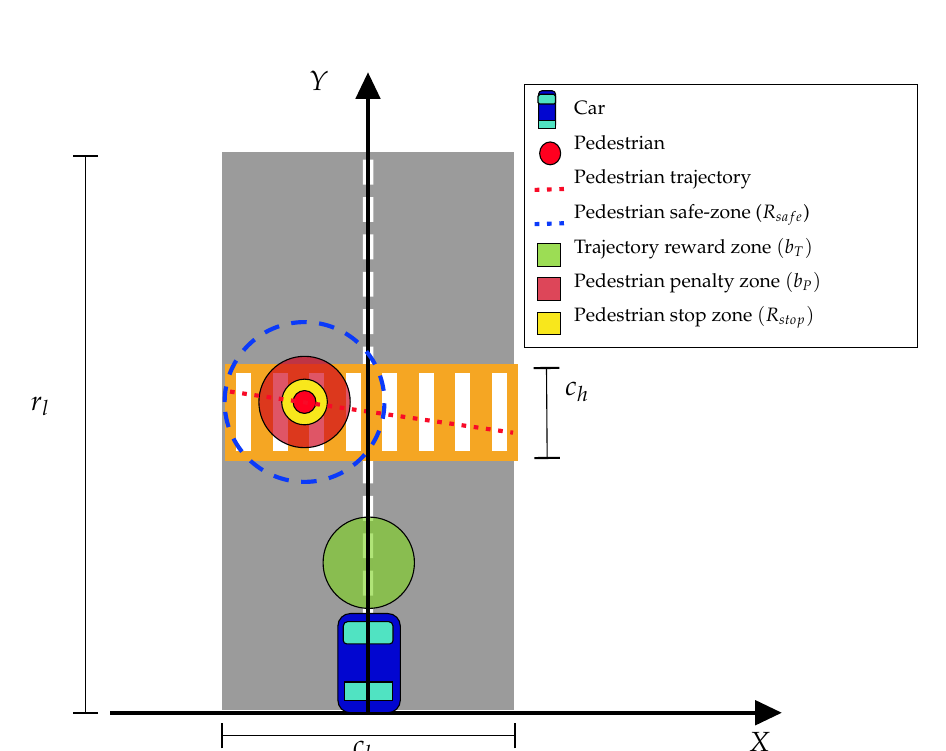
\begin{tikzpicture}[x=0.75pt,y=0.75pt,yscale=-1.1,xscale=1.1]
	%uncomment if require: \path (0,390); %set diagram left start at 0, and has height of 390
	
	%Straight Lines [id:da28584899643381045] 
	\draw [color={rgb, 255:red, 0; green, 0; blue, 0 }  ,draw opacity=1 ][fill={rgb, 255:red, 208; green, 2; blue, 27 }  ,fill opacity=1 ][line width=1.5]    (62,281) -- (352,281) ;
	\draw [shift={(356,281)}, rotate = 180] [fill={rgb, 255:red, 0; green, 0; blue, 0 }  ,fill opacity=1 ][line width=0.08]  [draw opacity=0] (11.61,-5.58) -- (0,0) -- (11.61,5.58) -- cycle    ;
	%Shape: Rectangle [id:dp5180666136146594] 
	\draw  [draw opacity=0][fill={rgb, 255:red, 155; green, 155; blue, 155 }  ,fill opacity=1 ] (238.84,280) -- (238.84,35.24) -- (110.84,35.24) -- (110.84,280) -- cycle ;
	%Straight Lines [id:da5379043576147695] 
	\draw [color={rgb, 255:red, 255; green, 255; blue, 255 }  ,draw opacity=1 ][fill={rgb, 255:red, 255; green, 255; blue, 255 }  ,fill opacity=1 ][line width=3.75]  [dash pattern={on 9pt off 4.5pt}]  (174.86,38.77) -- (174.82,277.88) ;
	%Shape: Rectangle [id:dp5984726439545023] 
	\draw  [draw opacity=0][fill={rgb, 255:red, 245; green, 166; blue, 35 }  ,fill opacity=1 ] (112.04,128.11) -- (240.71,128.11) -- (240.71,170.55) -- (112.04,170.55) -- cycle ;
	%Shape: Rectangle [id:dp3598384588943413] 
	\draw  [draw opacity=0][fill={rgb, 255:red, 255; green, 255; blue, 255 }  ,fill opacity=1 ] (117,132) -- (123.71,132) -- (123.71,166.45) -- (117,166.45) -- cycle ;
	%Shape: Rectangle [id:dp42660139670374453] 
	\draw  [draw opacity=0][fill={rgb, 255:red, 255; green, 255; blue, 255 }  ,fill opacity=1 ] (133,132) -- (139.71,132) -- (139.71,166.45) -- (133,166.45) -- cycle ;
	%Shape: Rectangle [id:dp4481761265320998] 
	\draw  [draw opacity=0][fill={rgb, 255:red, 255; green, 255; blue, 255 }  ,fill opacity=1 ] (149,132) -- (155.71,132) -- (155.71,166.45) -- (149,166.45) -- cycle ;
	%Shape: Rectangle [id:dp31095403090704243] 
	\draw  [draw opacity=0][fill={rgb, 255:red, 255; green, 255; blue, 255 }  ,fill opacity=1 ] (165,132) -- (171.71,132) -- (171.71,166.45) -- (165,166.45) -- cycle ;
	%Shape: Rectangle [id:dp9559285707259317] 
	\draw  [draw opacity=0][fill={rgb, 255:red, 255; green, 255; blue, 255 }  ,fill opacity=1 ] (181,132) -- (187.71,132) -- (187.71,166.45) -- (181,166.45) -- cycle ;
	%Shape: Rectangle [id:dp21507599882927209] 
	\draw  [draw opacity=0][fill={rgb, 255:red, 255; green, 255; blue, 255 }  ,fill opacity=1 ] (197,132) -- (203.71,132) -- (203.71,166.45) -- (197,166.45) -- cycle ;
	%Shape: Rectangle [id:dp041486191842157405] 
	\draw  [draw opacity=0][fill={rgb, 255:red, 255; green, 255; blue, 255 }  ,fill opacity=1 ] (213,132) -- (219.71,132) -- (219.71,166.45) -- (213,166.45) -- cycle ;
	%Shape: Rectangle [id:dp7164243700354131] 
	\draw  [draw opacity=0][fill={rgb, 255:red, 255; green, 255; blue, 255 }  ,fill opacity=1 ] (229,132) -- (235.71,132) -- (235.71,166.45) -- (229,166.45) -- cycle ;
	%Flowchart: Connector [id:dp4051301354453565] 
	\draw  [fill={rgb, 255:red, 208; green, 2; blue, 27 }  ,fill opacity=0.67 ] (127.02,144.89) .. controls (127.02,133.85) and (135.97,124.89) .. (147.02,124.89) .. controls (158.07,124.89) and (167.02,133.85) .. (167.02,144.89) .. controls (167.02,155.94) and (158.07,164.89) .. (147.02,164.89) .. controls (135.97,164.89) and (127.02,155.94) .. (127.02,144.89) -- cycle ;
	%Flowchart: Connector [id:dp9639108171950941] 
	\draw  [fill={rgb, 255:red, 248; green, 231; blue, 28 }  ,fill opacity=1 ] (137.02,144.89) .. controls (137.02,139.37) and (141.5,134.89) .. (147.02,134.89) .. controls (152.54,134.89) and (157.02,139.37) .. (157.02,144.89) .. controls (157.02,150.41) and (152.54,154.89) .. (147.02,154.89) .. controls (141.5,154.89) and (137.02,150.41) .. (137.02,144.89) -- cycle ;
	%Flowchart: Connector [id:dp4727997208074779] 
	\draw  [fill={rgb, 255:red, 255; green, 0; blue, 31 }  ,fill opacity=1 ] (142.02,144.89) .. controls (142.02,142.13) and (144.26,139.89) .. (147.02,139.89) .. controls (149.78,139.89) and (152.02,142.13) .. (152.02,144.89) .. controls (152.02,147.65) and (149.78,149.89) .. (147.02,149.89) .. controls (144.26,149.89) and (142.02,147.65) .. (142.02,144.89) -- cycle ;
	%Straight Lines [id:da041073960472972626] 
	\draw [color={rgb, 255:red, 248; green, 10; blue, 39 }  ,draw opacity=1 ][line width=1.5]  [dash pattern={on 1.69pt off 2.76pt}]  (114.37,140.33) -- (238.37,158.33) ;
	%Shape: Rectangle [id:dp15185882367612136] 
	\draw   (243.29,6) -- (415.5,6) -- (415.5,121.2) -- (243.29,121.2) -- cycle ;
	%Straight Lines [id:da7988843189062504] 
	\draw [color={rgb, 255:red, 248; green, 10; blue, 39 }  ,draw opacity=1 ][line width=1.5]  [dash pattern={on 1.69pt off 2.76pt}]  (247.82,52) -- (262.25,51.55) ;
	%Flowchart: Connector [id:dp7590194899937404] 
	\draw  [fill={rgb, 255:red, 255; green, 0; blue, 31 }  ,fill opacity=1 ] (250,36) .. controls (250,33.24) and (252.06,31) .. (254.61,31) .. controls (257.15,31) and (259.21,33.24) .. (259.21,36) .. controls (259.21,38.76) and (257.15,41) .. (254.61,41) .. controls (252.06,41) and (250,38.76) .. (250,36) -- cycle ;
	%Shape: Rectangle [id:dp20536350583269547] 
	\draw  [fill={rgb, 255:red, 126; green, 211; blue, 33 }  ,fill opacity=0.77 ] (249,75.5) -- (259,75.5) -- (259,85.5) -- (249,85.5) -- cycle ;
	%Shape: Rectangle [id:dp7543763695429884] 
	\draw  [fill={rgb, 255:red, 248; green, 231; blue, 28 }  ,fill opacity=1 ] (249,105.5) -- (259,105.5) -- (259,115.5) -- (249,115.5) -- cycle ;
	%Straight Lines [id:da9289731261582568] 
	\draw    (51,37) -- (51,281) ;
	\draw [shift={(51,281)}, rotate = 270] [color={rgb, 255:red, 0; green, 0; blue, 0 }  ][line width=0.75]    (0,5.59) -- (0,-5.59)   ;
	\draw [shift={(51,37)}, rotate = 270] [color={rgb, 255:red, 0; green, 0; blue, 0 }  ][line width=0.75]    (0,5.59) -- (0,-5.59)   ;
	%Straight Lines [id:da5378932582334461] 
	\draw    (239,291) -- (111,291) ;
	\draw [shift={(111,291)}, rotate = 360] [color={rgb, 255:red, 0; green, 0; blue, 0 }  ][line width=0.75]    (0,5.59) -- (0,-5.59)   ;
	\draw [shift={(239,291)}, rotate = 360] [color={rgb, 255:red, 0; green, 0; blue, 0 }  ][line width=0.75]    (0,5.59) -- (0,-5.59)   ;
	%Straight Lines [id:da33109690518949986] 
	\draw    (253,130) -- (253.29,169.41) ;
	\draw [shift={(253.29,169.41)}, rotate = 269.58] [color={rgb, 255:red, 0; green, 0; blue, 0 }  ][line width=0.75]    (0,5.59) -- (0,-5.59)   ;
	\draw [shift={(253,130)}, rotate = 269.58] [color={rgb, 255:red, 0; green, 0; blue, 0 }  ][line width=0.75]    (0,5.59) -- (0,-5.59)   ;
	%Flowchart: Connector [id:dp6794245955836984] 
	\draw  [fill={rgb, 255:red, 126; green, 211; blue, 33 }  ,fill opacity=0.61 ] (155.15,215.3) .. controls (155.15,204.25) and (164.1,195.3) .. (175.15,195.3) .. controls (186.2,195.3) and (195.15,204.25) .. (195.15,215.3) .. controls (195.15,226.34) and (186.2,235.3) .. (175.15,235.3) .. controls (164.1,235.3) and (155.15,226.34) .. (155.15,215.3) -- cycle ;
	%Rounded Rect [id:dp7752804182072381] 
	\draw  [fill={rgb, 255:red, 2; green, 6; blue, 208 }  ,fill opacity=1 ] (183.5,237.55) .. controls (186.52,237.55) and (188.97,240) .. (188.97,243.02) -- (188.97,275.53) .. controls (188.97,278.55) and (186.52,281) .. (183.5,281) -- (167.1,281) .. controls (164.08,281) and (161.63,278.55) .. (161.63,275.53) -- (161.63,243.02) .. controls (161.63,240) and (164.08,237.55) .. (167.1,237.55) -- cycle ;
	%Rounded Same Side Corner Rect [id:dp6191447553378682] 
	\draw  [fill={rgb, 255:red, 80; green, 227; blue, 194 }  ,fill opacity=1 ] (164,243.02) .. controls (164,241.94) and (164.88,241.06) .. (165.96,241.06) -- (183.82,241.06) .. controls (184.9,241.06) and (185.78,241.94) .. (185.78,243.02) -- (185.78,249.37) .. controls (185.78,250.18) and (185.12,250.85) .. (184.3,250.85) -- (165.48,250.85) .. controls (164.66,250.85) and (164,250.18) .. (164,249.37) -- cycle ;
	%Shape: Rectangle [id:dp15584204124077772] 
	\draw  [fill={rgb, 255:red, 80; green, 227; blue, 194 }  ,fill opacity=1 ] (164.5,267.55) -- (185.61,267.55) -- (185.61,275.53) -- (164.5,275.53) -- cycle ;
	%Shape: Rectangle [id:dp7507189763383675] 
	\draw  [fill={rgb, 255:red, 208; green, 2; blue, 27 }  ,fill opacity=0.73 ] (249,90.5) -- (259,90.5) -- (259,100.5) -- (249,100.5) -- cycle ;
	%Straight Lines [id:da3637152716158101] 
	\draw [color={rgb, 255:red, 0; green, 0; blue, 0 }  ,draw opacity=1 ][fill={rgb, 255:red, 208; green, 2; blue, 27 }  ,fill opacity=1 ][line width=1.5]    (174.82,281) -- (174.82,4.55) ;
	\draw [shift={(174.82,0.55)}, rotate = 450] [fill={rgb, 255:red, 0; green, 0; blue, 0 }  ,fill opacity=1 ][line width=0.08]  [draw opacity=0] (11.61,-5.58) -- (0,0) -- (11.61,5.58) -- cycle    ;
	%Shape: Circle [id:dp43448679482079333] 
	\draw  [color={rgb, 255:red, 11; green, 58; blue, 249 }  ,draw opacity=1 ][dash pattern={on 5.63pt off 4.5pt}][line width=1.5]  (112.02,144.89) .. controls (112.02,125.56) and (127.69,109.89) .. (147.02,109.89) .. controls (166.35,109.89) and (182.02,125.56) .. (182.02,144.89) .. controls (182.02,164.22) and (166.35,179.89) .. (147.02,179.89) .. controls (127.69,179.89) and (112.02,164.22) .. (112.02,144.89) -- cycle ;
	%Rounded Rect [id:dp8343624362355313] 
	\draw  [fill={rgb, 255:red, 2; green, 6; blue, 208 }  ,fill opacity=1 ] (255.47,8.59) .. controls (256.29,8.59) and (256.96,9.26) .. (256.96,10.08) -- (256.96,23.59) .. controls (256.96,24.41) and (256.29,25.08) .. (255.47,25.08) -- (251.01,25.08) .. controls (250.19,25.08) and (249.52,24.41) .. (249.52,23.59) -- (249.52,10.08) .. controls (249.52,9.26) and (250.19,8.59) .. (251.01,8.59) -- cycle ;
	%Shape: Rectangle [id:dp893778457744719] 
	\draw  [fill={rgb, 255:red, 80; green, 227; blue, 194 }  ,fill opacity=1 ] (249.52,21.61) -- (256.96,21.61) -- (256.96,25.08) -- (249.52,25.08) -- cycle ;
	%Rounded Same Side Corner Rect [id:dp9092713415456457] 
	\draw  [fill={rgb, 255:red, 80; green, 227; blue, 194 }  ,fill opacity=1 ] (249.29,10.97) .. controls (249.29,10.5) and (249.67,10.12) .. (250.14,10.12) -- (256.11,10.12) .. controls (256.58,10.12) and (256.96,10.5) .. (256.96,10.97) -- (256.96,13.72) .. controls (256.96,14.08) and (256.67,14.36) .. (256.32,14.36) -- (249.93,14.36) .. controls (249.58,14.36) and (249.29,14.08) .. (249.29,13.72) -- cycle ;
	%Straight Lines [id:da6017239908080465] 
	\draw [color={rgb, 255:red, 11; green, 58; blue, 249 }  ,draw opacity=1 ][line width=1.5]  [dash pattern={on 1.69pt off 2.76pt}]  (247.82,67) -- (262.25,66.55) ;
	
	% Text Node
	\draw (340.33,288.23) node [anchor=north west][inner sep=0.75pt]  [color={rgb, 255:red, 0; green, 0; blue, 0 }  ,opacity=1 ]  {$X$};
	% Text Node
	\draw (148,-1.24) node [anchor=north west][inner sep=0.75pt]  [color={rgb, 255:red, 0; green, 0; blue, 0 }  ,opacity=1 ]  {$Y$};
	% Text Node
	\draw (264,42) node [anchor=north west][inner sep=0.75pt]  [font=\scriptsize] [align=left] {Pedestrian trajectory};
	% Text Node
	\draw (264,27) node [anchor=north west][inner sep=0.75pt]  [font=\scriptsize] [align=left] {Pedestrian};
	% Text Node
	\draw (264,72) node [anchor=north west][inner sep=0.75pt]  [font=\scriptsize] [align=left] {Trajectory reward zone $(b_T)$ };
	% Text Node
	\draw (264,102) node [anchor=north west][inner sep=0.75pt]  [font=\scriptsize] [align=left] {Pedestrian stop zone $(R_{stop})$};
	% Text Node
	\draw (26,141.41) node [anchor=north west][inner sep=0.75pt]    {$r_{l}$};
	% Text Node
	\draw (167,292.41) node [anchor=north west][inner sep=0.75pt]    {$c_{l}$};
	% Text Node
	\draw (260,134.95) node [anchor=north west][inner sep=0.75pt]    {$c_{h}$};
	% Text Node
	\draw (264,87) node [anchor=north west][inner sep=0.75pt]  [font=\scriptsize] [align=left] {Pedestrian penalty zone $(b_P)$};
	% Text Node
	\draw (264,12) node [anchor=north west][inner sep=0.75pt]  [font=\scriptsize] [align=left] {Car};
	% Text Node
	\draw (264,57) node [anchor=north west][inner sep=0.75pt]  [font=\scriptsize] [align=left] {Pedestrian safe-zone ($R_{safe}$)};
	
	
\end{tikzpicture}
\caption{The intersection scenario for the pedestrian collision avoidance problem.}
\label{fig:scenario}
\end{figure}

More specifically, such scenario is composed by a straight road (with length $r_l= \SI{50}{\metre}$ and width $c_l=\SI{10}{\metre}$) and a crosswalk area (perpendicular to the road direction and placed at $\frac{r_l}{2}$ with a height of $c_h= \SI{2.5}{\metre}$). The vehicle has to follow the reference trajectory depicted as dashed white line in Fig.~\ref{fig:scenario}. During any travelling episode along the road, a pedestrian can unexpectedly cross the road when the traffic light allows the vehicle to proceed. 

\begin{figure}[ht]
\centering
\tikzset{every picture/.style={line width=0.75pt}} %set default line width to 0.75pt    
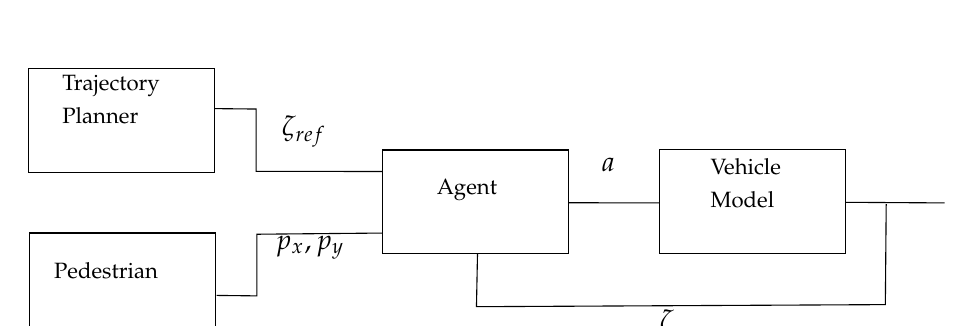
\begin{tikzpicture}[x=0.75pt,y=0.75pt,yscale=-1,xscale=1]
	%Shape: Rectangle [id:dp11457776888363957] 
	\draw   (77.13,55.6) -- (166.92,55.6) -- (166.92,105.6) -- (77.13,105.6) -- cycle ;
	%Shape: Rectangle [id:dp14347854375529412] 
	\draw   (247.67,94.93) -- (337.45,94.93) -- (337.45,144.93) -- (247.67,144.93) -- cycle ;
	%Shape: Rectangle [id:dp7094628553182183] 
	\draw   (381.17,94.9) -- (470.95,94.9) -- (470.95,144.9) -- (381.17,144.9) -- cycle ;
	%Shape: Rectangle [id:dp4842733937121826] 
	\draw   (77.67,134.93) -- (167.45,134.93) -- (167.45,184.93) -- (77.67,184.93) -- cycle ;
	%Straight Lines [id:da08669167245414444] 
	\draw    (167,75) -- (186.93,75.2) -- (186.93,105.2) -- (248.04,105.3) ;
	%Straight Lines [id:da9567989410678546] 
	\draw    (167.86,165) -- (187.3,165.22) -- (187.27,135.52) -- (247.84,134.95) ;
	%Straight Lines [id:da542342739302786] 
	\draw    (337.41,120.35) -- (381.09,120.43) ;
	%Straight Lines [id:da8872076809294023] 
	\draw    (471.05,120.14) -- (518.59,120.43) ;
	%Straight Lines [id:da75203079626961] 
	\draw    (490.5,121) -- (490.09,169.43) -- (293.09,170.43) -- (293.59,144.93) ;
	
	% Text Node
	\draw (92.3,57.67) node [anchor=north west][inner sep=0.75pt]   [align=left] {{\footnotesize Trajectory}\\{\footnotesize Planner}};
	% Text Node
	\draw (88.33,147.67) node [anchor=north west][inner sep=0.75pt]   [align=left] {{\footnotesize Pedestrian}};
	% Text Node
	\draw (272.7,107.5) node [anchor=north west][inner sep=0.75pt]   [align=left] {{\footnotesize Agent}};
	% Text Node
	\draw (404.67,97.5) node [anchor=north west][inner sep=0.75pt]   [align=left] {{\footnotesize Vehicle}\\{\footnotesize Model}};
	% Text Node
	\draw (198,77.33) node [anchor=north west][inner sep=0.75pt]    {${\textstyle \zeta _{ref}}$};
	% Text Node
	\draw (352.17,97.5) node [anchor=north west][inner sep=0.75pt]    {$a$};
	% Text Node
	\draw (380.17,170.5) node [anchor=north west][inner sep=0.75pt]    {$\zeta $};
	% Text Node
	\draw (195,135) node [anchor=north west][inner sep=0.75pt]    {$p_{x} ,p_{y}$};
\end{tikzpicture}
\caption{The agent-environment interaction for the pedestrian collision avoidance problem.}
\label{fig:principle_scheme}
\end{figure}
In such a situation, the trained DDPG based agent has to command the vehicle to avoid the inattentive pedestrian, and then taking again the reference trajectory. The overall RL system has been implemented in Matlab/Simulink. It consists of the DDPG based agent and its environment, that is to say, the vehicle itself, the pedestrian, and the trajectory planner (see Fig.~\ref{fig:principle_scheme}). The agent interacts with its environment through the vehicle acceleration and steering commands. The stochastic nature of the proposed system is linked to the unexpected behaviour of the pedestrian, who can enter the crosswalk area at any time and by following an unknown path within such area. In other words, while learning to follow the reference trajectory, the effect of the selected sequence of actions on the expected return $G_t$ is subject to such unknown pedestrian behaviour.
%are not deterministically  we do not have the $P(\cdot|s,a)$ especially around the pedestrian crossing and this makes it necessary to use learning techniques to approximate the \textit{Q-function} such as \textit{DDPG}. The reward $R(\cdot|s,a)$, on the other hand, is deterministic and is carefully designed to guide the \texit{Q-learning} process so that the agent is able to perform his task.
%In the remaining part of this section, all the elements of the proposed RL system are described, including the reward function definition.
%the various components of the RL system are described in detail. In particular the model of the car and the trajectory planner are reported in section \ref{sub_sec:3-a} and \ref{sub_sec:3-b} respectively, the behaviour of the pedestrian is described in section \ref{sub_sec:3-c}, the details on the implementation of the agent are reported in section \ref{sub_sec:3-d} and the reward shaping is characterized in section \ref{sub_sec:3-e}.
\begin{figure}[ht]
\centering
\includegraphics[scale=0.5]{figure/Part2/Chapter5/Images/model_vehicle.jpg} 
\caption{The vehicle model.}
\label{fig:model_vehicle}
\end{figure}

\subsection{The vehicle dynamics model}
\label{sub_sec:3-a}
Vehicles operating in an urban environment can be represented via a kinematic based model~\cite{bicycle_Frazzoli}. In this work, we adopt the model described in~\cite{bicycle_Borrelli}, which is shown in \mbox{Fig.~\ref{fig:model_vehicle}}. In such model, the wheels do not slip at their contact point with the ground since both the velocity and the acceleration values are assumed to be low. 
The following set of nonlinear continuous time equations describes the selected model for the vehicles dynamics
\begin{subequations}
\label{vehicmodel}
\begin{align}
	\frac{dx(t)}{dt} &=v(t) \cos (\psi(t)+\beta(t)), \\
	\frac{dy(t)}{dt} &=v(t) \sin (\psi(t)+\beta(t)), \\
	\frac{d\psi(t)}{dt} &=\frac{v(t)}{l_{r}} \sin (\beta(t)), \\
	\frac{dv(t)}{dt} &= \mu(t), 
\end{align}
\end{subequations}
\noindent with
\begin{subequations}[resume]
\begin{align}
	\beta(t) &=\tan ^{-1}\left(\frac{l_{r}}{l_{f}+l_{r}} \tan \left(\delta_{f}(t)\right)\right).
\end{align}
\end{subequations}
In our work, for the sake of simplicity, we make explicit the time  dependence of the state and action variables only when they are introduced for the first time. In the presented model, $x$ and $y$ are the vehicle mass-center coordinates in an inertial frame, while the heading angle and the speed of the vehicle mass-center are $\psi$ and $v$. The distance from the vehicle mass-center to the front and rear axles are $l_f= \SI{1.738}{\metre}$ and $l_r=\SI{1.105}{\metre}$, respectively. Moreover, $\beta$ represents the angle of the current mass-center velocity vector with respect to the longitudinal axis of
the vehicle, while $\mu$ is the mass-center acceleration along such velocity vector. The control inputs are the front steering angles $\delta_f$ and the acceleration $\mu$. In other words, we assume that the vehicle is a front wheel steering vehicle, hence $\delta_r \equiv 0$.   

The vehicle dynamics model~\eqref{vehicmodel}  can be expressed in a vector form as follows
\begin{equation}
\begin{aligned}
	\frac{d\zeta}{dt}  & = f(\zeta,u), \\
	%\zeta  \in & \mathbf{R}^{n_\zeta} , u \in \mathbf{R}^{n_u}. \\
\end{aligned}
\end{equation}
\noindent where $\zeta=[x,y, \psi, v]' \in {R}^{4}$ and $u=[\delta_f ,\mu]' \in {R}^{2}$ represent the state and input vector, respectively (note that the \mbox{symbol $'$} denotes the transpose operator).


\subsection{The pedestrian position and the trajectory planner}
\label{sub_sec:3-b}
The pedestrian position measurements are described by the following equations
\begin{equation}
\begin{cases} p_x(t)=p_{x_0}+v_{x_p}\cdot t+\eta_{ \rm x}, \\ p_y(t)=p_{y_0}+v_{y_p}\cdot t +\eta_{\rm y},
\end{cases} 
\end{equation}
where
\begin{itemize}
\item $p_{x_0}$ and $p_{y_0}$ are the  coordinates of the pedestrian initial position. 
\item $v_{x_p}$ and $v_{y_p}$ are the component of the pedestrian velocity vector and are assumed to be constant.
\item $\eta_{\rm x} \sim \mathcal{N}\left(0, \sigma_{\rm \eta_x}^{2}\right)$ and $ \eta_{\rm y} \sim \mathcal{N}\left(0, \sigma_{\rm \eta_y}^{2}\right)$ represent the Gaussian noise of the vehicle on-board devices (e.g., RADAR sensors), responsible for the acquisition of the current pedestrian position $p = [p_x, p_y]'$. 
%By considering that the pedestrian position can be acquired by vehicle on-board devices (e.g., RADAR sensors), we add their related measurement Gaussian noise $\eta_{radar} \sim \mathcal{N}\left(0, \sigma_{radar}^{2}\right)$ when computing the current pedestrian position $p(t) = [p_x(t), p_y(t)]'$.
\end{itemize}

We set the values of the pedestrian initial and final position vectors, $p_0=[p_{x_0}, p_{y_0}]'$ and $p_f=[p_{x_f}, p_{y_f}]'$, as follows
\begin{itemize}
\item $p_{x_f} $ and $p_{x_0}$ are chosen according to a Bernoulli random variable $b \sim \operatorname{Bern}(0.5)$ as
\begin{equation}
	\centering   
	\begin{aligned}
		p_{x_f} & =-(2b-1)\cdot\frac{c_l}{2}, \\
		p_{x_0} & =(2b-1)\cdot\frac{c_l}{2};
	\end{aligned}
\end{equation}
\item $p_{y_f} $ and $p_{y_0}$ are Gaussian random variables, namely $p_{y_f} \sim \mathcal{N}\left(\frac{r_l}{2}, \sigma_{y}^2\right)$, $p_{y_0} \sim \mathcal{N}\left(\frac{r_l}{2},\sigma_{y}^2\right)$.
\end{itemize}

The variances $\sigma_{\rm \eta_x}^2 = \sigma_{\rm \eta_y}^2$ and $\sigma_{y}^2$ are set to $\SI{0.2}{m^2}$ and $\SI{1}{m^2}$, respectively. The pedestrian moves along a straight path within the crosswalk area at the constant velocity vector $v_p=[v_{x_p}, v_{y_p}]'$.
%, which can be easily computed once we set the departure and arrival times ($t_0$ and $t_f$) for the given episode. They are chosen in such a way that the vehicle can potentially hit the pedestrian along its trajectory. 




%\begin{equation}
%    v_p=\frac{p_f-p_0 }{t_f-t_0}
%\end{equation}
%where $p_f=[p_{x_f} \quad p_{y_f}]'$ and $p_0=[p_{x_0} \quad p_{y_0}]'$. Where   $p_{x_f} $ and $p_{x_0}$ are chosen according to a Bernoulli random variable $b \sim \operatorname{Bern}(0.5)$ as:
%\begin{equation}
% \centering   
%\begin{aligned}
%    p_{x_f} & =-(2b-1)\cdot\frac{c_l}{2} \\
%    p_{x_0} & =(2b-1)\cdot\frac{c_l}{2}
%\end{aligned}
%\end{equation}
%and $p_{y_f} $ and $p_{y_0}$ are gaussian random variables namely $p_{y_f} \sim \mathcal{N}\left(\frac{r_l}{2}, \sigma_{y}\right)$, $p_{y_0} \sim \mathcal{N}\left(\frac{r_l}{2},\sigma_{y}\right)$.




%\subsection{Trajectory planner}
\label{sub_sec:3-c}
The local trajectory planner calculates a uniform rectilinear motion  $\zeta_{\rm ref}(t)=[x_{ref}(t) ,y_{\rm ref}(t),\psi_{\rm ref}(t),v_{\rm ref}(t)]' $ that the vehicle has to follow
\begin{equation}
\centering
\begin{aligned}
	x_{\rm ref}(t)&=0, \\ 
	y_{\rm ref}(t) &=  v_{\rm const} \cdot \sin{\psi_{\rm const}} \cdot t, \\
	v_{\rm ref}(t) &= v_{\rm const}, \\
	\psi_{\rm ref}(t) &= \psi_{\rm const}.
\end{aligned}
\end{equation}



In our training episodes, we set the reference cruise velocity $v_{\rm const}$ to $\SI{10}{\frac{\metre}{\sec}}$ and the reference heading direction $\psi_{\rm ref}$ to $\frac{\pi}{2}$ \SI{}{\radian} . 



\subsection{The proposed DDPG based agent architecture}
\label{sub_sec:3-d}
The proposed DDPG based agent processes the following two error vectors
\begin{equation}
\centering   
\begin{aligned}
	e_T(t) &= [ x_{\rm ref}(t)-x(t), y_{\rm ref}(t)-y(t)]',  \\
	e_P(t) &= [p_x(t)-x(t), p_y(t)-y(t)]',  \\
\end{aligned}
\end{equation}
\noindent where $e_T$ and $e_P$ are  the error of the autonomous vehicle with respect to the reference trajectory and its relative distance to the pedestrian, respectively. Hence, the continuous time state and action vectors for the DDPG based agent can be expressed as follows  
\begin{equation}
\label{Eq:state_action}
\begin{aligned}
	s(t)=&[e_T(t), \frac{de_T(t)}{dt}, e_P(t), \frac{de_P(t)}{dt}]', \\
	a(t)=&[\delta_f(t), \mu(t)]'.
\end{aligned}
\end{equation}

In this work, we use the agent architecture shown in Fig.~\ref{fig:act_crit}. The neural networks are composed of fully connected layers with $N_{\rm nn}=100$ number of neurons.
%in Fig. \ref{Critic_Network} and Fig. \ref{Actor_Network}, where {\rm FC} and {\rm TL} represent the fully connected layers and activation function $\tanh$ layers.
%Each fully connected layer consists of $N_{nn}=100$ number of neurons.
%\begin{figure}[ht]
%	\centering
%	\includegraphics[scale=0.23]{Images/nn.jpg} 
%	\caption{Critic network of the proposed DDPG based agent.}
%	\label{Critic_Network}
%\end{figure}
%\begin{figure}[ht]
%	\centering
%	\includegraphics[scale=0.23]{Images/act.png} 
%	\caption{Actor network of the proposed DDPG based agent.}
%	\label{Actor_Network}
%\end{figure}
The DDPG algorithm~\cite{DDPG} is used to train the agent's neural networks. During each episode, the vehicle operates at the intersection scenario shown in Fig.~\ref{fig:scenario}, while the DDPG based agent updates the parameters of both the actor and the critic neural networks. At each step of the episode, a tuple $\left(s_t, a_t, r_{t+1}, s_{t+1}\right)$ is stored into a circular buffer, which can hold up to \mbox{$N_{\rm buff}=10000$} samples. The actor and critic parameters are updated by using a mini-batch of $N_{\rm batch}=256$ samples, randomly selected  from the circular buffer. 
%The discount factor $\gamma$ and the smoothing factor $\rho$ are set to $0.99$ and $0.001$, respectively. 

%Furthermore, to increase the exploration capabilities during at least the early phase of the training process, an Ornstein-Uhlenbeck noise \cite{DDPG_noise} is added to the two action components with a life time, expressed in episode, given by the following expression 
%\begin{equation}
%    N_{\rm noise}=4\frac{\log 0.5}{\log \left( 1-\tau_{\rm rate} \right)},
%\end{equation}
%with the decay rate $\tau_{\rm rate}$ set to $10^{-4}$.



%in particular for this agent with two actions, we set the variance of each action to a equal value while using the same decay rate $\tau_{rate}=1e^{-4}$ for both variances. With the chosen decay rate the number of steps $N_{noise}$ for which the action is subjected to the noise can be calculated with the following equation:



\subsection{Reward function shaping}
\label{subsec:reward_shaping}
\label{sub_sec:3-e}
The reward function selection was driven by the two competing objectives to be achieved by the agent: following a reference trajectory and avoiding unexpected pedestrian crossings. The proposed reward function is composed of five deterministic terms, and depends on all the components of the $s$ and $a$ vectors~\eqref{Eq:state_action}, with the exception of their time derivative elements. The tuning of their parameters was the result of a trial and error approach. 
%The relevant physical parameters of the reward function terms are shown in Fig. \ref{fig:scenario}.


To encourage the agent to maintain the reference trajectory, we introduce the following exponential function as the first addend of the reward function (see Fig.~\ref{fig:traj_rew})
\begin{equation} \label{rewfirst}
r_{{T}}(s)=r_{\rm max}\cdot \  (e^{- \alpha_{T} \cdot \| e_T \|}), 
\end{equation}
where $r_{\rm max}=15$ is the maximum desired reward in correspondence of the zero trajectory error ($\|e_T\|=0$) and $\alpha_T$ is a constant gain defined as follows
\begin{equation}
\alpha_{T} = -
\frac{\ln\frac{r*}{r_{\rm max}}}{b_T\quad},
\end{equation}
where $b_T$ corresponds to all the trajectory error values $e_T$  with $r_T \le r^*$ (in our case $r^*=1$).

Fig.~\ref{fig:traj_rew} shows the traversal section of the two-variable reward function graph~\eqref{rewfirst}, centered on the zero trajectory error. Note that the reward function term~\eqref{rewfirst} is symmetric with respect to the origin, and has its level sets centered on the zero error trajectory.

As shown in Fig.~\ref{fig:traj_rew}, two different values of $b_T$ are considered
\begin{equation}
b_{T}= \begin{cases} b_{T_{\rm ped}} & \text{if } \|e_P\| \le R_{ \rm safe} \\  b_{T_{\rm traj}} & \text{if } \|e_P\| > R_{\rm safe},
\end{cases} 
\end{equation}
with $b_{T_{\rm ped}}=\SI{27.8}{\metre}$, $b_{T_{\rm traj}} =\SI{1.35}{\metre}$, and $R_{\rm safe} = \SI{5}{\metre}$ is a radius defining a safe zone around pedestrian. This way, as soon as the vehicle enters the safe zone, being very close to the reference trajectory becomes less important, and the agent is forced to focus on the primary objective of avoiding the inattentive pedestrian.
%is a  conventional boundary of the trajectory error value  obtained for a fixed trajectory  reward value $r_T(s)=r*$ and is depicted in Fig.\ref{fig:traj_rew} for $r*=1$. This function allows to obtain good performance in terms of trajectory tracking. To increase manoeuvring space in proximity of pedestrian the $b_T$ value are changed as:
%\begin{equation}
%    b_{T}= \begin{cases} b_{T_{ped}} & \text{if } \|e_P\| < R_{safe} \\  b_{T_{traj}} & \text{if } \|e_P\| \geq R_{safe}
%\end{cases} 
%\end{equation}
%\color{blue}
%$b_{T_{ped}}=27.8$, $b_{T_{traj}} =1.35$
%$b_P = 5.5$
%\color{black}
%$b_{T_{ped}}\geq b_{T_{traj}}$ and $R_{safe} = \SI{5}{\metre}$ is a radius defining a safe zone around pedestrian. The effect of this change in the reward function is reported in Fig.\ref{fig:traj_rew}
\begin{figure}[ht]
	\centering
	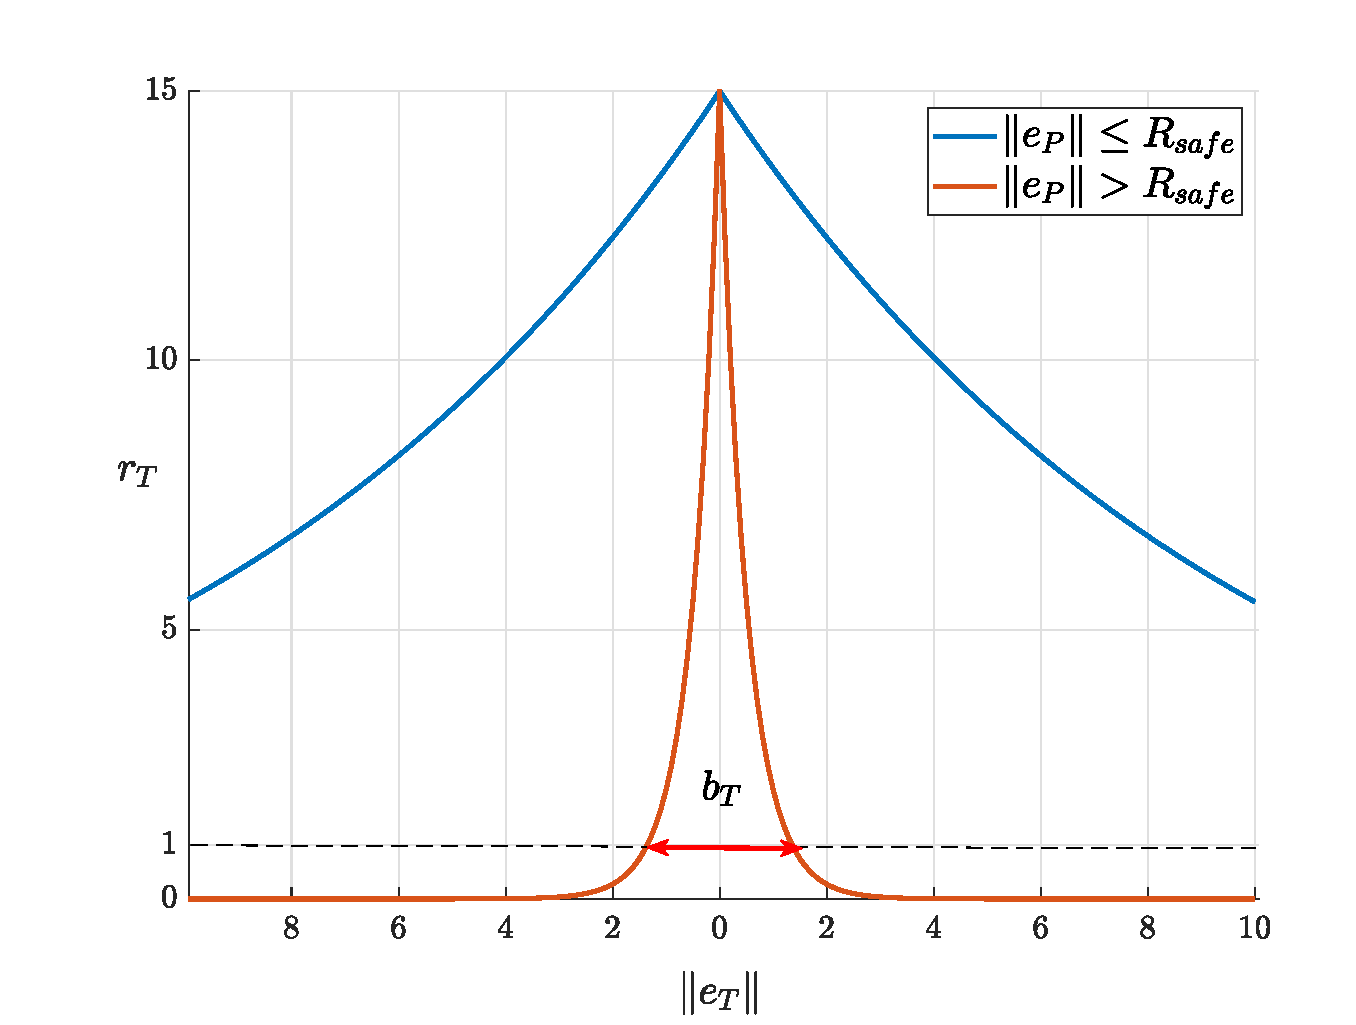
\includegraphics[scale=0.5]{figure/Part2/Chapter5/Images/reward_trajectory_final.eps}
	\caption{Trajectory reward function term.}
	\label{fig:traj_rew}
\end{figure} 

A similar approach is used to define the reward function term for the pedestrian collision avoidance, In particular, we introduce the following exponential function (see Fig.~\ref{fig:ped_rew})
\begin{equation}
	r_P (s) = 
	p_{ \rm max} (e^{ \alpha_{P} \cdot  \| e_P \|}),
\end{equation}
where  $p_{\rm max}=-15$  is the maximum penalty in correspondence of the pedestrian position and $\alpha_{P}$ is a constant defined as follows
\begin{equation}
	\alpha_{P} =  -\frac{\ln\frac{p*}{p_{\rm max}}}{b_P}. \quad 
\end{equation}

Like the previous term,  $b_{P}$ corresponds to all the relative distance values $e_P$ to the pedestrian  with $r_P \le p^*$ (in our case $p^*=1$ and $b_P = \SI{5.5}{\metre}$). As shown in Fig.~\ref{fig:ped_rew}, the pedestrian reward term is only activated when $\|e_P\| \le R_{\rm safe}$.
%is a conventional boundary on pedestrian distance for a fixed penalty $r_P(s)=p*$ and is depicted in Fig. \ref{fig:ped_rew} for $p*=-1$. Pedestrian contribution to total reward is considered only for $\|e_P\|<R_{safe}$
Both trajectory and pedestrian reward term parameters are carefully chosen in order to assure an appropriate reward function shape in the proximity of the pedestrian position as shown in Fig.~\ref{fig:traj_rew_3D}, where the maximum reward values are placed at the border of the pedestrian safe zone. 

\begin{figure}[ht]
	\centering
	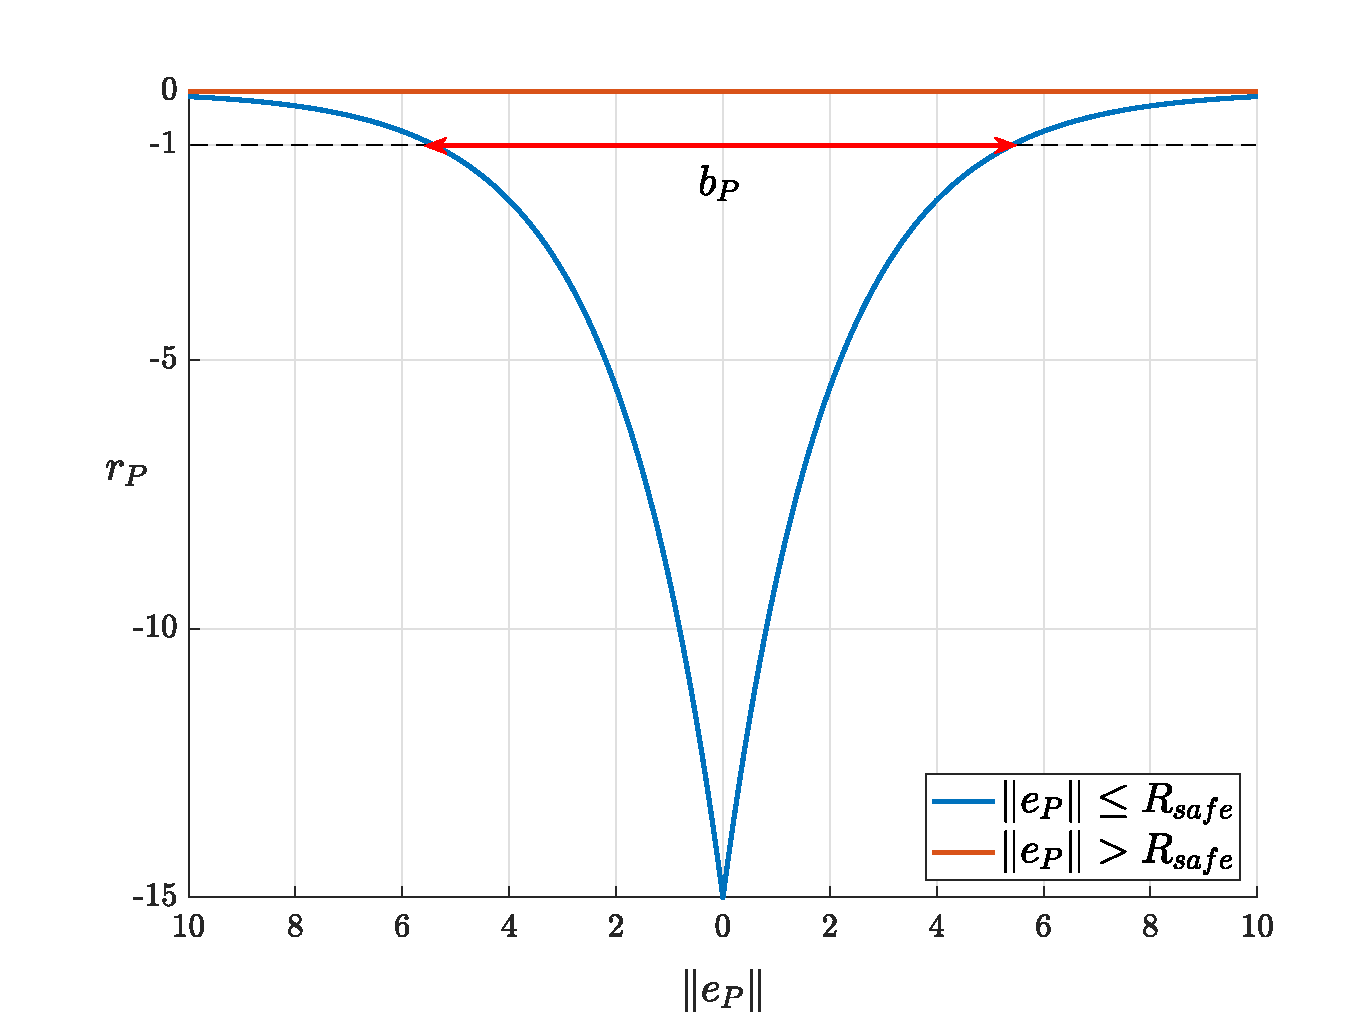
\includegraphics[scale=0.5]{figure/Part2/Chapter5/Images/Reward_pedestrian_final.eps}
	\caption{Pedestrian reward function term.}
	\label{fig:ped_rew}
\end{figure}
\begin{figure}[ht]
	\centering
	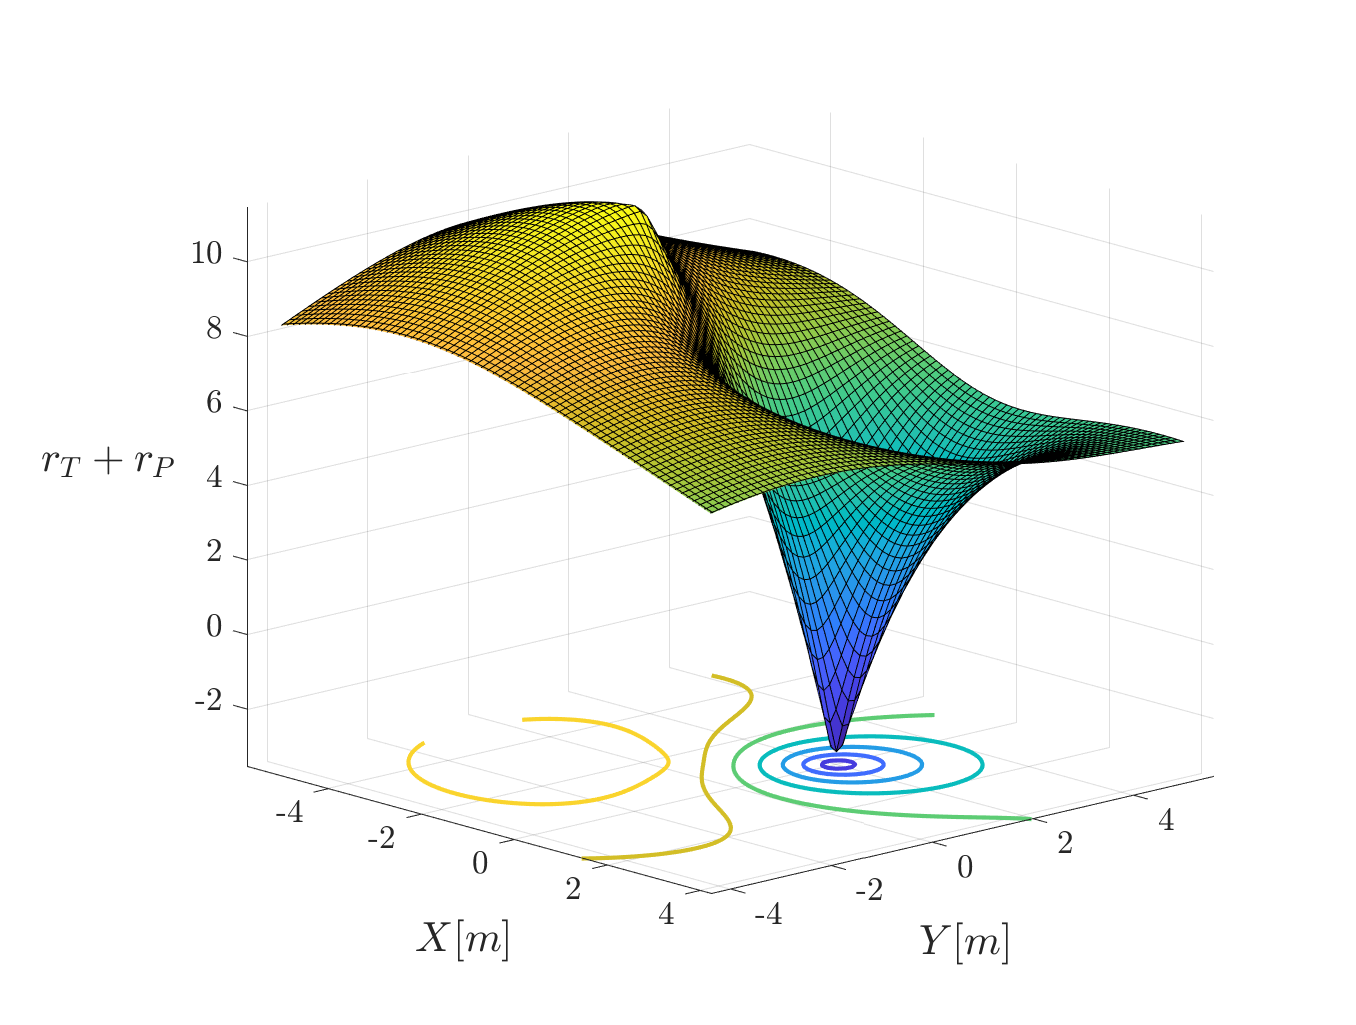
\includegraphics[scale=0.5]{figure/Part2/Chapter5/Images/Total_3D_reward.eps}
	\caption{Combination of the trajectory and pedestrian reward function terms.}
	\label{fig:traj_rew_3D}
\end{figure}


The third reward function term is linked to the selected actions 
\begin{equation}
	r_{\rm act}(s) = - \alpha_a \cdot (\| a_t-a_{t-1} \|^2 ), \\
\end{equation} 
where $\alpha_a = 10$ is the weight parameter for the control action. It aims at endorsing smooth variations of the control actions between two consecutive time slots.
%where $a$ and $a_{-1}$ represent the actual action taken and the previous one taken at the previous time step.

Two further reward terms are added to strengthen the learning process. In particular, the training episode is stopped  whenever a predetermined distance from the reference trajectory $E_{\rm max}$ is reached or the pedestrian stopping zone is entered. The following two terms are defined 
\begin{equation}
	r_{{\rm end}_P(s)}=\begin{cases}p_{P} & \text{if } e_P \leq R_{ \rm stop}, \\ 0, & \text{otherwise},
	\end{cases} 
\end{equation}
\begin{equation}
	r_{{\rm end}_T}(s)=\begin{cases} p_T & \text{if } e_{T} > E_{\rm max},  \\ 0, & \text{otherwise}. 
	\end{cases} 
\end{equation}
We set the following values: $p_{P}=p_{T}=-50$, $R_{\rm stop}=\SI{1}{\metre}$, and $E_{\rm max}=\SI{15}{\metre}$. To sum up, the complete reward function is given by the following expression
\begin{equation}
	\begin{aligned}
		r(s,a)=r_{{T}}(s)+ r_{P}(s) + r_{{\rm end}_P}(s) + r_{{\rm end}_T}(s) +  r_{\rm act}(a).
	\end{aligned}
\end{equation}
\label{sub_sec:3-e}


%\color{blue}
%Moreover to ensure safety a circle safe area with radius $R_{safe}= \SI{1}{\metre}$ is created around the pedestrian position. This abstraction is exploited in the reward shaping phase as  reported in subsection \ref{subsec:reward_shaping}.

%A stop condition is raised when the vehicle enters inside a circumference of radius $R_{safe}=\SI{1}{\metre}$. This early stopping helps the agent to improve the learning of pedestrian avoidance.



\section{Numerical simulations and results}
\label{sec:Results and conclusions}
In this section, we discuss the training process of the DDPG based agent previously described, and then we show the performance achieved by the resulting trained agent.

As expected, the training process  was influenced by three main factors: (i) the architecture of the actor and the critic neural networks (along with the values assigned to their hyper-parameters); (ii) the DDPG algorithm configuration parameters (e.g., the size of the  mini-batch $N_{\rm batch}$); the reward function definition.
%(e.g., the number of , a, see the paragraph \ref{sub_sec:3-d}.
%The choice of the actor and critic neural network hyper-parameters, see the paragraph \ref{sub_sec:3-d}.
%The reward function definition, see the paragraph %\ref{subsec:reward_shaping}.
For instance, a small mini-batch of samples  did not allow exploring the state/action space in an efficient way. In such a case, both the quality and the speed of the overall learning process were affected. Such issues were also observed when we defined and shaped the reward function. Indeed, the reward function presented in the paragraph~\ref{sub_sec:3-e} was the result of an engineering effort supported by a trial and error approach.
%resulted in a slow learning process. thus the network parameters are updated in a less precise way and the overall learning process slows down. %The decay rate $\tau_{\rm rate}$ has to be set in a proper way, so that the agent can also exploit what is has already experienced. 
%The most influential hyper-parameters  are the size of the  mini-batch $N_{\rm batch}$ and the decay rate $\tau_{ \rm rate}$ of the noise variance for the selected action $a_t$. Indeed,a small mini-batch of samples $N_{\rm batch}$ does not allow exploring the state/action space in an efficient way, thus the network parameters are updated in a less precise way and the overall learning process slows down. The decay rate $\tau_{\rm rate}$ has to be set in a proper way, so that the agent can also exploit what is has already experienced. 
%overall learning process can benefit from the exploit the of the noise variance, on the other hand, if not properly chosen may cause for the noise to affect excessively the action even when the actor's neural network has already understood a good behaviour. 
%The shape of the reward function  can considerably affect both the quality and the speed of the learning process. For instance, the reward functions shown in Fig. \ref{fig:traj_rew} and Fig. \ref{fig:ped_rew} have a very high derivative near the zero error. As a consequence, the agent can determine its correct behaviour more quickly.
%presented in the section \ref{sub_sec:3-e} is characterised by the fact that the limit of the derivative in correspondence of zero error is very high (ideally infinite) which means that small variations around the zero error determine abrupt drops in the reward, allowing the agent to  better understand the correct behaviour in less time. 

The training process was carried out for $N_{\rm ep}=6500$ episodes. 
%\st{where $N_{\rm ep}>N_{\rm noise}$. It was noted that, even when the noise added to the action was negligible, the randomness used for the mini-batch of transitions led to an improvement in the agent performance.} 
In addition, we set the sampling time  $T_s$ to $\SI{0.05}{\sec}$, the maximum time of each episode $T_{\rm sim}$  to $\SI{5}{\sec}$, and the discount factor $\gamma$ to $0.99$.
%of the tuple space sampling determines an improvement in the agent's performance.  
The outcome of the training process is shown in Fig.~\ref{fig:training_result}, where the moving mean value and the moving standard deviation of the total reward computed over the last $N_{\rm av}=20$ episodes are plotted. At the beginning of the training phase, the agent learnt to follow quickly the reference trajectory up to the beginning of the  pedestrian crosswalk area (thanks to  the exploration capabilities of the DDPG algorithm~\cite{DDPG}). After being stuck for a short period, the learning process continued, but more slowly. In this phase, we also observed increasing standard deviation values of the total reward (mainly due to the occurrence of pedestrian hits within the crosswalk area). At the end, the total reward mean value stabilised, while the related standard deviation decreased significantly. In particular, the agent learnt to avoid the pedestrian, and the residual standard deviation was only due to the distance of the vehicle from the reference trajectory. We also observed that the agent learnt to follow the reference trajectory beyond the pedestrian crosswalk area.

\begin{figure}
	\centering
	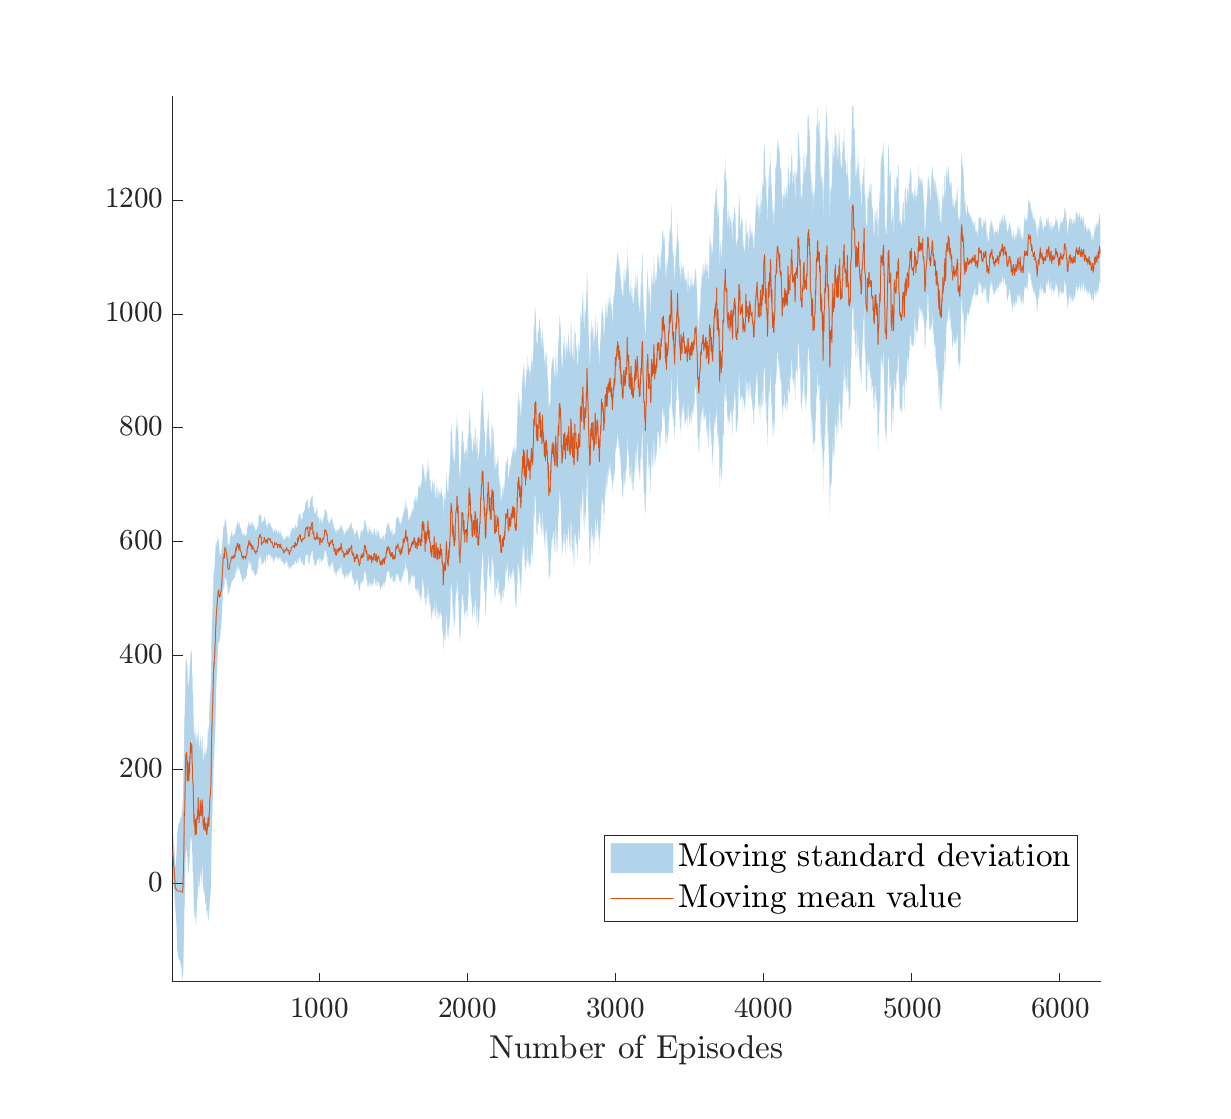
\includegraphics[scale=0.75]{figure/Part2/Chapter5/Images/std_plot.eps} 
	\caption{Moving mean value and standard deviation of the total reward during the training process.}
	\label{fig:training_result}
\end{figure}
%the blue line represents the total reward of each episode, the red line is the moving average total reward over the last $N_{\rm av}=20$ episodes, and the yellow line is the critic estimate $Q_0$ of the discounted long-term total reward at the beginning  of each episode. It is possible to distinguish four main portions in the training process as highlighted in Fig. \ref{fig:training_result} : (i) the first one in which the total reward for each episode is approximately zero since the agent explores the state space with pure random actions; (ii) the second one in which there is an improvement in the total reward thanks to the fact that the agent is able to follow the reference trajectory up to the beginning of the  pedestrian crosswalk area; (iii)  the third one characterized by slow improvement and high variance for the total reward (due to the occurrence of pedestrian hits within the crosswalk area); (iv) the fourth one where the total reward values stabilise since the agent handles more properly all the various pedestrian crossing directions, besides tracking the reference trajectory. %characterized by lowest variance and highest mean reward. We can also notice how $Q_0$ slowly converges to the experienced average total reward at the end of the training process.



\begin{figure}
	\centering
	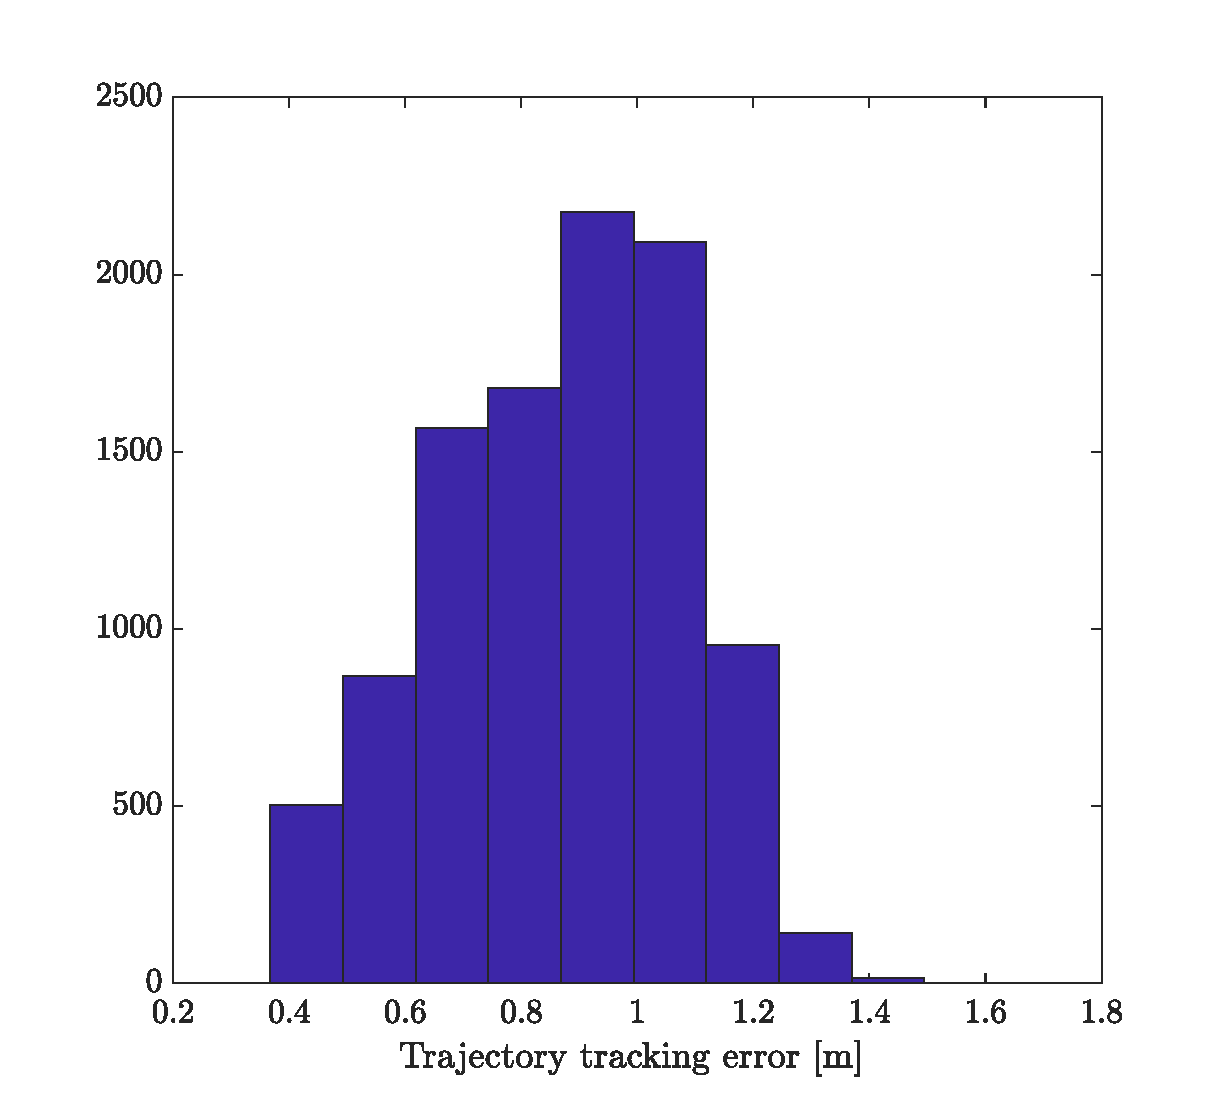
\includegraphics[scale=0.4]{figure/Part2/Chapter5/Images/err_traj.eps} 
	\caption{Maximum trajectory tracking error distribution.}
	\label{fig:episodetest}
\end{figure}


\begin{figure}
	\centering
	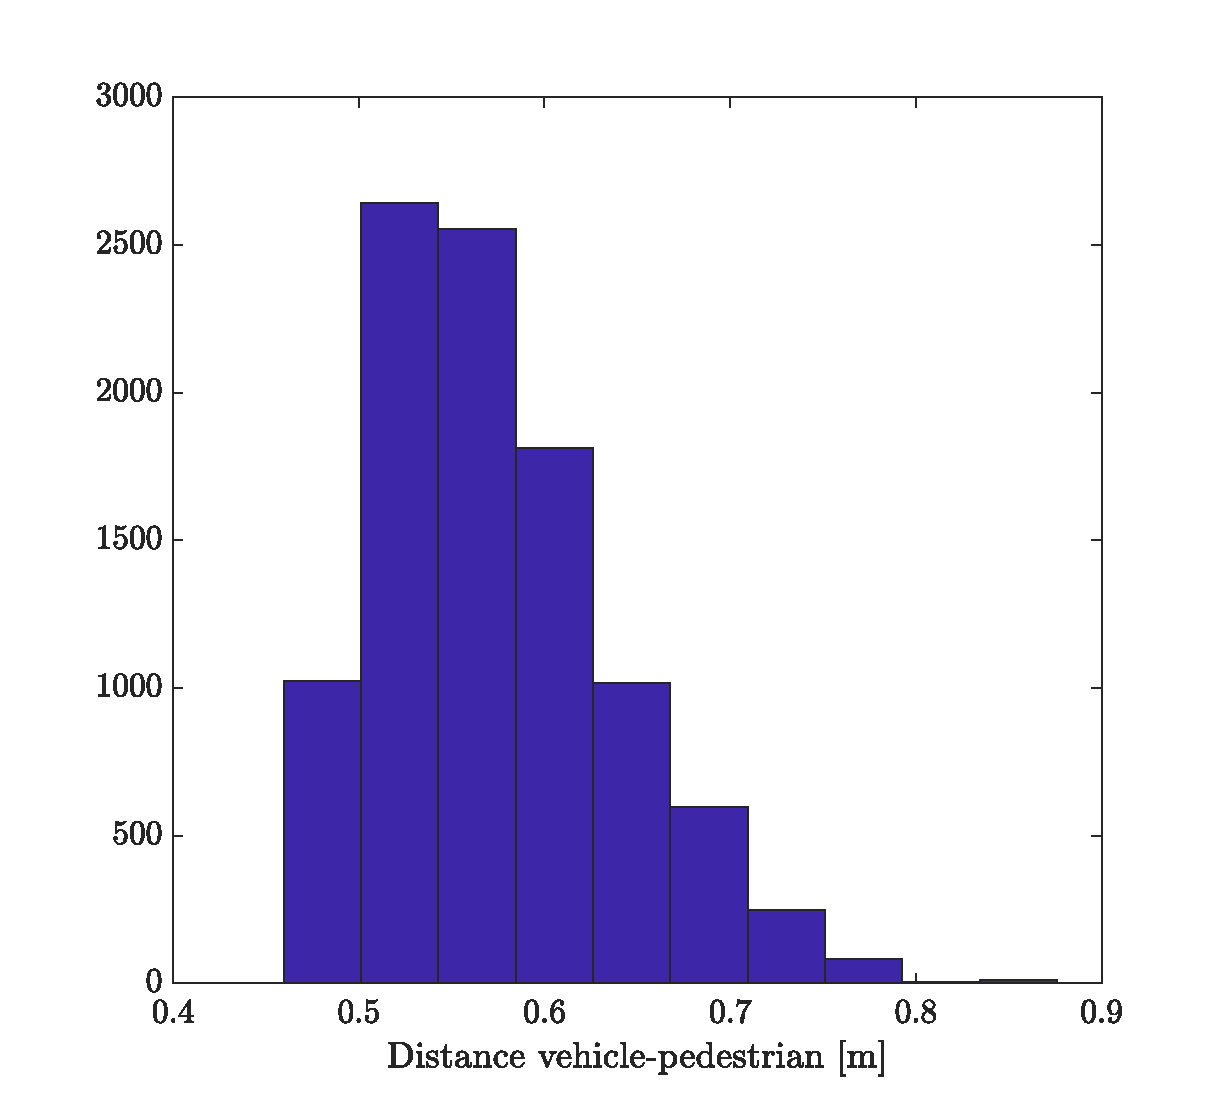
\includegraphics[scale=0.4]{figure/Part2/Chapter5/Images/err_ped_estrian.eps}
	\caption{Minimum vehicle-pedestrian distance distribution.}
	\label{fig:errorepisode}
\end{figure}

After the training phase, we tested our agent for $N_{\rm test} = 10000$ episodes, in which we observed zero pedestrian hits and adequate trajectory tracking performance. Fig.~\ref{fig:episodetest} shows the distribution of the maximum trajectory tracking error, while Fig.~\ref{fig:errorepisode} plots the distribution of the minimum vehicle-pedestrian distance.

%\color{blue}
%@Luigi: nella figura 12, una label dorebbe essere $e_{\psi}$.
%\color{black}

%\color{blue}
%Conviene in questo paragrafo indicare il valore dei parametri usato nelle simulazioni: ad esempio,
%$\sigma_{radar}= \SI{0.2}{m}$, $t_0$, $t_f$, $\sigma_x$, $\sigma_y$, $c_l$, $r_l$, $b$. Da discutere.
%\color{black}

\newpage
\section{Chapter Summary}


In conclusion, the implementation of the Deep Deterministic Policy Gradient (DDPG) algorithm for pedestrian collision avoidance in autonomous vehicles has showcased substantial potential in enhancing urban navigation safety. Through detailed numerical analysis, the algorithm demonstrated a commendable capability in reducing collision risks with pedestrians, a critical aspect of autonomous vehicle deployment in densely populated areas. The numerical results underline the algorithm's effectiveness, showing marked improvements in decision-making accuracy under various simulated urban scenarios. However, it's the inherent adaptability and learning efficiency of the DDPG algorithm that stand out, suggesting that with ongoing refinement, its application could lead to even safer and more precise autonomous driving solutions. By leveraging the strengths and addressing the limitations identified in this study, the DDPG algorithm can significantly contribute to the evolution of autonomous driving technologies, ensuring a safer coexistence between autonomous vehicles and urban pedestrians.

\chapter{A Machine Learning-Control Approach for Cybersecurity}
\label{Chapter:4}

% *** HERE STARTS THE GLOSSARY ENTRIES DEFINITION ***
% \newabbreviation{tag}{displayed acronym}{description/long name}
% \newabbreviation{}{}{}


This chapter introduces a sophisticated defense and mitigation control scheme designed to protect autonomous vehicles  during overtaking maneuvers from cyber-attacks, including Replay Attacks and Denial of Service attacks. The proposed Informative Model Predictive Scheme  architecture aims to detect and mitigate these attacks, thereby preserving the safety and integrity of AV control systems. The scheme leverages Machine Learning for attack detection, employing a Constrained Support Vector Machine classifier informed by Nonlinear Model Predictive Control data to distinguish between normal operation and various attack scenarios effectively. This approach is innovative in its adaptability to time-varying or nonlinear dynamics and its ability to implement countermeasures dynamically, showcasing a novel direction in enhancing vehicular cybersecurity. Through simulation and analysis, this chapter seeks to underline the effectiveness of the I-MPS in ensuring the safe and reliable operation of autonomous vehicles in the face of increasingly sophisticated cyber threats.

\newpage


\section{Control Strategy Architecture and Problem Formulation}
\label{sec:second}
%
We consider the~\gls{av} control architecture, depicted in Fig.~\ref{fig:architecture_attacker}, consisting on a trajectory planner which computes a high-level plan for the incoming overtaking, the proposed~\gls{imps} which is in charge of tracking the plan provided by trajectory planner, the sensory system which is responsible of providing relevant information to the on-board systems regarding the vehicle's velocity, position, acceleration and heading and  an \gls{ekf} which is in charge of filtering out the measurement noise from the measurements coming from the upstream sensory system. We further assume: (i) no model mismatch between the model used by the \gls{imps} and the mismatch for the vehicle's dynamics and (ii) that a hacker can inject \gls{ra} or \gls{dos} attacks by accessing the vehicle's CAN gateway (e.g., through Bluetooth, radio data, telematics)~\cite{bozdal2020evaluation}. 



\begin{figure}[ht]
	\centering
	
		\tikzset{every picture/.style={line width=0.9pt}} %set default line width to 0.75pt        
		\begin{tikzpicture}[x=0.75pt,y=0.75pt,yscale=-1.4,xscale=1.4]
		%uncomment if require: \path (0,300); %set diagram left start at 0, and has height of 300
		
		
		\fill[gray!30!white] (10,50) rectangle (230,140);
		\fill[gray!30!white] (10,195) rectangle (330,130);
		\node[] at (50,160) {AV control  };
		\node[] at (50,174) {architecture};
		%Shape: Rectangle [id:dp6121517022672165] 
		\draw   (19,59) -- (94.3,59) -- (94.3,108.46) -- (19,108.46) -- cycle ;
		%Shape: Rectangle [id:dp958930299715433] 
		\draw   (131.96,59) -- (207.26,59) -- (207.26,108.46) -- (131.96,108.46) -- cycle ;
		%Shape: Rectangle [id:dp44779293427709854] 
		\draw   (131.96,141.43) -- (207.26,141.43) -- (207.26,190.89) -- (131.96,190.89) -- cycle ;
		%Shape: Rectangle [id:dp5634290255034515] 
		\draw   (244.91,59) -- (320.22,59) -- (320.22,108.46) -- (244.91,108.46) -- cycle ;
		%Shape: Rectangle [id:dp5757397298802769] 
		\draw   (244.91,141.43) -- (320.22,141.43) -- (320.22,190.89) -- (244.91,190.89) -- cycle ;
		%Straight Lines [id:da9864178721017116] 
		\draw    (94.3,83.73) -- (129.96,83.73) ;
		\draw [shift={(131.96,83.73)}, rotate = 180] [color={rgb, 255:red, 0; green, 0; blue, 0 }  ][line width=0.75]    (10.93,-3.29) .. controls (6.95,-1.4) and (3.31,-0.3) .. (0,0) .. controls (3.31,0.3) and (6.95,1.4) .. (10.93,3.29)   ;
		%Straight Lines [id:da09220870807386605] 
		\draw    (207.26,83.73) -- (243.54,84.51) ;
		\draw [shift={(245.54,84.55)}, rotate = 181.23] [color={rgb, 255:red, 0; green, 0; blue, 0 }  ][line width=0.75]    (10.93,-3.29) .. controls (6.95,-1.4) and (3.31,-0.3) .. (0,0) .. controls (3.31,0.3) and (6.95,1.4) .. (10.93,3.29)   ;
		%Straight Lines [id:da35189222289389144] 
		\draw    (244.91,166.16) -- (209.26,166.16) ;
		\draw [shift={(207.26,166.16)}, rotate = 360] [color={rgb, 255:red, 0; green, 0; blue, 0 }  ][line width=0.75]    (10.93,-3.29) .. controls (6.95,-1.4) and (3.31,-0.3) .. (0,0) .. controls (3.31,0.3) and (6.95,1.4) .. (10.93,3.29)   ;
		%Straight Lines [id:da8394517684121314] 
		\draw    (320.22,83.73) -- (339.05,83.73) ;
		%Straight Lines [id:da04036512434087469] 
		\draw    (339.05,83.73) -- (339.05,166.16) ;
		%Straight Lines [id:da37873235038513076] 
		\draw    (320.22,166.16) -- (339.05,166.16) ;
		%Straight Lines [id:da23549189407989646] 
		\draw    (169.61,141.43) -- (169.61,110.46) ;
		\draw [shift={(169.61,108.46)}, rotate = 450] [color={rgb, 255:red, 0; green, 0; blue, 0 }  ][line width=0.75]    (10.93,-3.29) .. controls (6.95,-1.4) and (3.31,-0.3) .. (0,0) .. controls (3.31,0.3) and (6.95,1.4) .. (10.93,3.29)   ;
		%Image [id:dp6840101759405377] 
		\draw (226.59,214.03) node  {\includegraphics[width=19.3pt,height=26.81pt]{figure/Part2/Chapter6/Figures/cyber_attacker.jpg}};
		%Straight Lines [id:da35054905401151815] 
		\draw [color={rgb, 255:red, 208; green, 2; blue, 27 }  ,draw opacity=1 ]   (225.96,196.69) -- (226.11,169.43) ;
		\draw [shift={(226.12,167.43)}, rotate = 450.31] [color={rgb, 255:red, 208; green, 2; blue, 27 }  ,draw opacity=1 ][line width=0.75]    (10.93,-3.29) .. controls (6.95,-1.4) and (3.31,-0.3) .. (0,0) .. controls (3.31,0.3) and (6.95,1.4) .. (10.93,3.29)   ;
		
		% Text Node
		\draw (19.28,70) node [anchor=north west][inner sep=0.75pt]   [align=left] {\begin{minipage}[lt]{50.513188pt}\setlength\topsep{0pt}
			\begin{center}
			Trajectory \\Planner
			\end{center}
			
			\end{minipage}};
		% Text Node
		\draw (149,70) node [anchor=north west][inner sep=0.75pt]   [align=left] {\gls{imps} \\ Sec.~\ref{sec:I-MPS}};
		% Text Node
		\draw (254.19,63) node [anchor=north west][inner sep=0.75pt]   [align=left] {\begin{minipage}[lt]{37.855940000000004pt}\setlength\topsep{0pt}
			\begin{center}
			\vspace{0.2cm}
			Vehicle \\
			Sec.~\ref{sub_sec:vehicle_model}
			\end{center}
			
			\end{minipage}};
		% Text Node
		\draw (150,153) node [anchor=north west][inner sep=0.75pt]   [align=left] { \gls{ekf} \\ Sec.~\ref{subsec:Estimator}};
		% Text Node
		\draw (260,143) node [anchor=north west][inner sep=0.75pt]   [align=left] {Sensory \\ System \\ Sec.~\ref{sub_sec:Sensory_system}};
		% Text Node
		\draw (243,205) node [anchor=north west][inner sep=0.75pt]   [align=left] {\textcolor[rgb]{0.82,0.01,0.11}{HACKER}\\ Sec.~\ref{sub_sec:attacker_model}};
		
		
		\end{tikzpicture}

	\caption{ \gls{av} control architecture. The hacker corrupts the outputs of the sensory system.}
	\label{fig:architecture_attacker}
\end{figure}
%




\subsection{Vehicle Model}
\label{sub_sec:vehicle_model}
%
Vehicles operating in an urban environment can be modeled via a kinematic bicycle based model~\cite{bicycle_Borrelli},~\cite{Bicycle_model_2}. In such model, the wheels do not slip at their contact point with the ground since both the velocity and the acceleration values are assumed to be low. Furthermore,  we assume that the vehicle is a front wheel steering vehicle.

Thus, the vehicle dynamics are given by~\cite{bicycle_Borrelli}
%
\begin{subequations}
	\label{eq:vehicmodel}
	\begin{align}
		\dot{x} &= v \cos \big(\psi+\beta\big),\\
		\dot{y}  &= v \sin \big(\psi+\beta\big),\\
		\dot{\psi}  &= \frac{v}{l_{r}} \sin \beta,\\
		\dot{v}  &= a,
	\end{align}
\end{subequations}
% Se usi il commento non hai bisogno di istanziare un \noindent. Troppi comandi non sono raccomandabili perché in alcune condizioni potrebbero scemunire il compilatore. Col commento ottieni il risultato di segmentare il testo per, deduco, migliorare la leggibilità senza generare indentazioni tipiche di un nuovo capoverso.
where $x$ and $y$ are the coordinates of the vehicle mass-center in an inertial frame, $\psi$ is the heading angle of the vehicle mass-center, $v$ is the velocity of the vehicle mass-center, $a$ is the mass-center acceleration, $\beta =\arctan\Big(l_{r}\tan \delta_f\slash(l_{f}+l_{r}) \Big)$ is the side slip angle of the vehicle, and $l_f$ and $l_r$ are the distances of the front and rear axles from the mass-center, respectively, $\delta_f$  and  $a$ the steering angle and acceleration, respectively. 

In what follows, $\zeta=\begin{bmatrix}x & y & \psi & v\end{bmatrix}^\top \in \mathbb{R}^{4 } $ and \mbox{$u=\begin{bmatrix}\delta_f & a\end{bmatrix}^\top \in \mathbb{R}^{2 }$ } will be used to indicate the state and the input vectors of the system, respectively.

\subsection{Sensory System}
\label{sub_sec:Sensory_system}
%
The state measurements supplied by the Sensory System module are subject to additive noise and are modeled as 
% se lasci una riga poi nel pdf c'è uno spazio troppo grande
\begin{equation}\label{eq:sensor_measurements}
	\zeta_m = \zeta + \eta,
\end{equation}
%	
where $\zeta_m=\begin{bmatrix} x_m & y_m & \psi_m & v_m \end{bmatrix}^\top$ and $\eta=\begin{bmatrix} \eta_x & \eta_y & \eta_\psi & \eta_v \end{bmatrix}^\top$, with $\eta_x$, $\eta_y$, $\eta_{\psi}$ and $\eta_v$ being zero mean, white Gaussian noises. The state measurements vector $\zeta_m$ is the whole knowledge accessible by the hacker. 

\subsection{Hacker Model}
\label{sub_sec:attacker_model}
%
In this subsection we define how a hacker can corrupt the measurements, as depicted in Fig.~\ref{fig:architecture_attacker}. For both attacks, $t_a$ and $T_d$ will indicate the time at which an attack starts and its duration, respectively.
%
\paragraph{Replay Attacks}
\glspl{ra} consist of a recording and a replay phase. During the recording phase, the hacker stores the past measurements, which in the replay phase are injected into the system. The \gls{ra} model is given by~\cite{teixeira2015secure}
%
\begin{equation} \label{eq:replay_model}
	\zeta^{\rm RA}_{m}(t) = \begin{cases}  \zeta_m(t-T_d), & \mbox{if } t \in \big[t_a,t_a+ T_d\big], \\ \zeta_m(t), & \mbox{otherwise}.  \end{cases}
\end{equation} 
%	
with the recording taking place in the time interval~\mbox{$\big[t_a-T_d,t_a\big]$}.
%
\paragraph{Denial of Service Attacks}
In this case, the hacker interrupts the data stream between the Sensory System and the \gls{ekf}. In real vehicles the \gls{ecu}, where the Controller block is implemented, typically holds the last useful data in the local memory which is then used in place of the expected new ones when they are not available. The model for \gls{dos} attacks is~\cite{schenato2009zero}
%
\begin{equation}
	\label{eq:Dos_model}
	\zeta^{\rm DoS}_{m}(t)=%
	\begin{cases}
		\zeta_m\big(t\big)\big|_{t=t_a}, & \mbox{if } t \in \big[t_a,t_a+T_d\big], \\ \zeta_m(t), & \mbox{otherwise}.
	\end{cases}
\end{equation} 
%
That is, the effect of the \gls{dos} attack consists in resending the sensor measured at the time $t=t_a$ during the time interval $\big[t_a,t_a+T_d\big]$.
\subsection{\gls{ekf}}
\label{subsec:Estimator}
%
In this work, the \gls{ekf}~\cite{EKF_3} provides the estimates $\hat\zeta$ of the vehicle's dynamics to the \gls{imps} block. Although the use of this estimator could improve the detectability of a cyber-attack~\cite{ekf_1_attack}, in the case under investigation, it is in charge only to provide the state estimation to the \gls{nmpc}.




%%% END SECTION ============================================================

%%% START SECTION ==========================================================

\section{I-MPS}
\label{sec:I-MPS}
%
Fig.~\ref{fig:I-NMPC} shows the proposed \gls{imps}. It includes three interconnected modules: the Detector, the Mitigator and an \gls{nmpc}. However, the architecture and the deriving scheme are general enough so as to allow other types of Model Based Controller such as, e.g., LTI-MPC, \gls{ltvmpc}, \gls{lpvmpc}. A discrete-time setting is assumed with $k$ being the discrete-time variable and $T_s$ being the sampling time such that $t=kT_s$.
%
\begin{figure}[H]
	\centering
	


\tikzset{every picture/.style={line width=0.75pt}} %set default line width to 0.75pt        

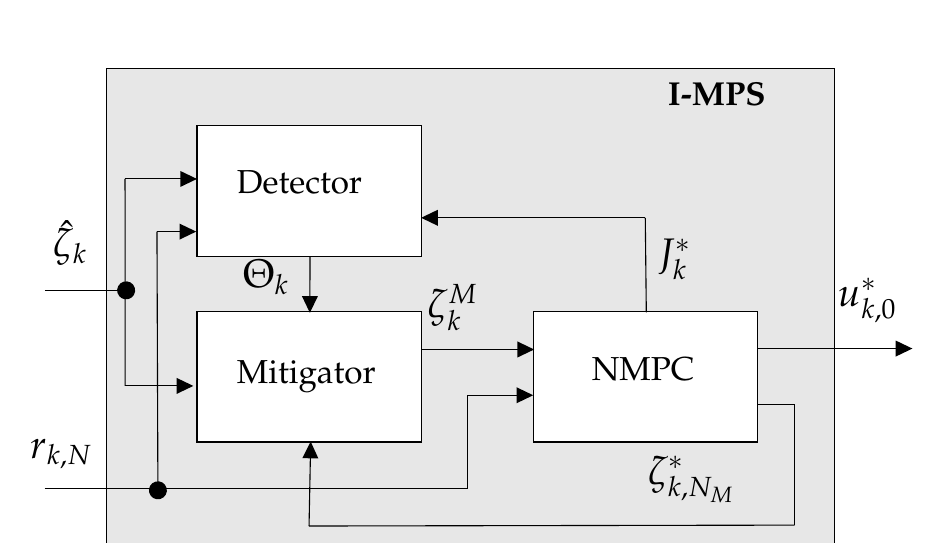
\begin{tikzpicture}[x=0.75pt,y=0.75pt,yscale=-0.9,xscale=0.9]
%uncomment if require: \path (0,300); %set diagram left start at 0, and has height of 300

%Shape: Rectangle [id:dp07321239801052792] 
\draw  [color={rgb, 255:red, 0; green, 0; blue, 0 }  ,draw opacity=1 ][fill={rgb, 255:red, 231; green, 231; blue, 231 }  ,fill opacity=1 ] (121.5,30) -- (511.5,30) -- (511.5,290) -- (121.5,290) -- cycle ;
%Shape: Rectangle [id:dp1563881976892849] 
\draw  [fill={rgb, 255:red, 255; green, 255; blue, 255 }  ,fill opacity=1 ] (170,160) -- (290,160) -- (290,230) -- (170,230) -- cycle ;
%Shape: Rectangle [id:dp978555336465935] 
\draw  [fill={rgb, 255:red, 255; green, 255; blue, 255 }  ,fill opacity=1 ] (170,60.67) -- (290,60.67) -- (290,130.67) -- (170,130.67) -- cycle ;
%Shape: Rectangle [id:dp6438542779108847] 
\draw  [fill={rgb, 255:red, 255; green, 255; blue, 255 }  ,fill opacity=1 ] (350,160) -- (470,160) -- (470,230) -- (350,230) -- cycle ;
%Straight Lines [id:da2661535299648963] 
\draw    (290.5,180.5) -- (347.5,180.5) ;
\draw [shift={(350.5,180.5)}, rotate = 180] [fill={rgb, 255:red, 0; green, 0; blue, 0 }  ][line width=0.08]  [draw opacity=0] (8.93,-4.29) -- (0,0) -- (8.93,4.29) -- cycle    ;
%Straight Lines [id:da9975743928269731] 
\draw    (470,180) -- (550,180) ;
\draw [shift={(553,180)}, rotate = 180] [fill={rgb, 255:red, 0; green, 0; blue, 0 }  ][line width=0.08]  [draw opacity=0] (8.93,-4.29) -- (0,0) -- (8.93,4.29) -- cycle    ;
%Straight Lines [id:da45105295619600305] 
\draw    (410,110) -- (410.55,160.67) ;
%Straight Lines [id:da31332759246635855] 
\draw    (410,110) -- (293,110) ;
\draw [shift={(290,110)}, rotate = 360] [fill={rgb, 255:red, 0; green, 0; blue, 0 }  ][line width=0.08]  [draw opacity=0] (8.93,-4.29) -- (0,0) -- (8.93,4.29) -- cycle    ;
%Straight Lines [id:da6831976187030333] 
\draw    (131.5,89.2) -- (131.55,200) ;
%Straight Lines [id:da5381627981193056] 
\draw    (131.5,89.2) -- (167,89.2) ;
\draw [shift={(170,89.2)}, rotate = 180] [fill={rgb, 255:red, 0; green, 0; blue, 0 }  ][line width=0.08]  [draw opacity=0] (8.93,-4.29) -- (0,0) -- (8.93,4.29) -- cycle    ;
%Straight Lines [id:da9898851017884422] 
\draw    (490,210) -- (490,274.52) ;
%Straight Lines [id:da424908054336965] 
\draw    (470,210) -- (490,210) ;
%Straight Lines [id:da2810640697891009] 
\draw    (230,275) -- (230.82,232.82) ;
\draw [shift={(230.88,229.82)}, rotate = 451.11] [fill={rgb, 255:red, 0; green, 0; blue, 0 }  ][line width=0.08]  [draw opacity=0] (8.93,-4.29) -- (0,0) -- (8.93,4.29) -- cycle    ;
%Straight Lines [id:da4824194165524387] 
\draw    (230,275) -- (490,274.52) ;
%Straight Lines [id:da6654648688677554] 
\draw    (230.5,130.91) -- (230.46,157.85) ;
\draw [shift={(230.45,160.85)}, rotate = 270.09000000000003] [fill={rgb, 255:red, 0; green, 0; blue, 0 }  ][line width=0.08]  [draw opacity=0] (8.93,-4.29) -- (0,0) -- (8.93,4.29) -- cycle    ;
%Shape: Circle [id:dp22585331850262147] 
\draw  [fill={rgb, 255:red, 0; green, 0; blue, 0 }  ,fill opacity=1 ] (127.76,150.09) .. controls (127.07,147.7) and (128.45,145.2) .. (130.84,144.51) .. controls (133.23,143.82) and (135.73,145.2) .. (136.42,147.59) .. controls (137.12,149.98) and (135.74,152.48) .. (133.34,153.17) .. controls (130.95,153.87) and (128.45,152.49) .. (127.76,150.09) -- cycle ;
%Straight Lines [id:da506959418744912] 
\draw    (88.55,148.84) -- (132.09,148.84) ;
%Straight Lines [id:da9298485020674954] 
\draw    (131.55,200) -- (165.05,200) ;
\draw [shift={(168.05,200)}, rotate = 180] [fill={rgb, 255:red, 0; green, 0; blue, 0 }  ][line width=0.08]  [draw opacity=0] (8.93,-4.29) -- (0,0) -- (8.93,4.29) -- cycle    ;
%Straight Lines [id:da32869903555712465] 
\draw    (88.5,255) -- (315,255) ;
%Straight Lines [id:da035880638063171544] 
\draw    (315,205) -- (315,255) ;
%Straight Lines [id:da6563089432200115] 
\draw    (315,205) -- (347,205) ;
\draw [shift={(350,205)}, rotate = 180] [fill={rgb, 255:red, 0; green, 0; blue, 0 }  ][line width=0.08]  [draw opacity=0] (8.93,-4.29) -- (0,0) -- (8.93,4.29) -- cycle    ;
%Shape: Circle [id:dp41684320512129514] 
\draw  [fill={rgb, 255:red, 0; green, 0; blue, 0 }  ,fill opacity=1 ] (144.76,257.14) .. controls (144.07,254.74) and (145.45,252.24) .. (147.84,251.55) .. controls (150.23,250.86) and (152.73,252.24) .. (153.42,254.64) .. controls (154.12,257.03) and (152.74,259.53) .. (150.34,260.22) .. controls (147.95,260.91) and (145.45,259.53) .. (144.76,257.14) -- cycle ;
%Straight Lines [id:da35344859328738143] 
\draw    (148.59,117.39) -- (149.09,255.89) ;
%Straight Lines [id:da8249585929292025] 
\draw    (148.59,117.39) -- (166.59,117.39) ;
\draw [shift={(169.59,117.39)}, rotate = 180] [fill={rgb, 255:red, 0; green, 0; blue, 0 }  ][line width=0.08]  [draw opacity=0] (8.93,-4.29) -- (0,0) -- (8.93,4.29) -- cycle    ;

% Text Node
\draw (420.67,36.17) node [anchor=north west][inner sep=0.75pt]  [font=\large] [align=left] {\textbf{I-MPS}};
% Text Node
\draw (380,183) node [anchor=north west][inner sep=0.75pt]  [font=\large] [align=left] {NMPC};
% Text Node
\draw (190,83) node [anchor=north west][inner sep=0.75pt]  [font=\large] [align=left] {Detector};
% Text Node
\draw (190,185) node [anchor=north west][inner sep=0.75pt]  [font=\large] [align=left] {Mitigator};
% Text Node
\draw (79.67,227) node [anchor=north west][inner sep=0.75pt]  [font=\Large]  {$r_{k,N}$};
% Text Node
\draw (91.5,110) node [anchor=north west][inner sep=0.75pt]  [font=\Large]  {$\hat{\zeta }_{k}$};
% Text Node
\draw (292,144) node [anchor=north west][inner sep=0.75pt]  [font=\Large]  {${\zeta^{M}_{k}}$};
% Text Node
\draw (512,141) node [anchor=north west][inner sep=0.75pt]  [font=\Large]  {$u^{*}_{k,0}$};
% Text Node
\draw (415,120) node [anchor=north west][inner sep=0.75pt]  [font=\Large]  {$J^{*}_{k}$};
% Text Node
\draw (193,131) node [anchor=north west][inner sep=0.75pt]  [font=\Large]  {$\Theta _{k}$};
% Text Node
\draw (410,236.17) node [anchor=north west][inner sep=0.75pt]  [font=\Large]  {$\zeta ^{*}_{k,N_M}$};


\end{tikzpicture}
	\caption{\gls{imps} architecture.}
	\label{fig:I-NMPC}
\end{figure}
%
\subsection{NMPC for Trajectory Tracking}
\label{subsec:NMPC}
%
The \gls{nmpc} is solved at each $k$ by minimizing the cost function
\begin{align}\label{eq:J}
	\nonumber J_k=&\sum_{i=k}^{k+N}(\zeta_i-r_i)^\top L(\zeta_i-r_i)\\&+\sum_{i=k}^{k+N-1} (u_i-u_{i-1})^\top S(u_i-u_{i-1}) + u_i^\top R u_i,
\end{align}
across the prediction horizon $N$ and where \mbox{$\zeta_{i}=\begin{bmatrix} x_i & y_i & \psi_i & v_i \end{bmatrix}^\top$} is the $i$-th future state vector of the vehicle's dynamic model used by the \gls{nmpc}, $r_i$ is the $i$-th future reference provided by the trajectory planner through the sequence $r_{k,N} = \big\{r_k, \ldots, r_{k+N}\big\}$, $u_i$ is the $i$-th \gls{nmpc} future outputs, and $L$, $S$ and $R$ are suitable weighting matrices of appropriate dimensions by which the control input performances are taken into account. 

The discrete-time optimization problem is solved by discretizing the continuous time model~\eqref{eq:vehicmodel} assuming a piecewise constant control $u(\tau)=u_k$, with $\tau \in \big[t_k,t_{k+1}\big[$, and then using the multiple shooting method~\cite{NMPC_1} which yields the constraint
\begin{equation}\label{eq:con_integrator}
	\zeta_{k+1}-\Xi(\zeta_k,u_k) = 0,
\end{equation}
where $\Xi(\zeta_k,u_k)$ is the $4$-th order Runge-Kutta integrator for the integration of the system dynamics over the shooting interval. Furthermore, the initial state is included as constraint into the optimization problem as follow
\begin{equation}\label{eq:con_init}
	\zeta_k -{\zeta}^M_{k}=0,
\end{equation}
where ${\zeta}^M_{k}$ is the Mitigator output.



The physical limitations of the control input regarding the  minimum  and  maximum values, $u_{\mathrm{min}}$ and $u_{\mathrm{max}}$, respectively, and slew-rates, $\dot{u}_{\mathrm{min}}$ and $\dot{u}_{\mathrm{max}}$, respectively, that the actuation system is capable of, can be taken into account as
\begin{subequations}\label{eq:con_u_tot}
	\begin{align}
		u_{\mathrm{min}} \leq u_k  \leq& u_{\mathrm{max}},\label{eq:con_u}\\
		\dot u_{\mathrm{min}} \leq \dot{u}_k \leq& \dot{u}_{\mathrm{max}}.\label{eq:con_dot_u}
	\end{align}
\end{subequations}


Ultimately, the \gls{nmpc} computes
%
\begin{argmini}|s|
	{\zeta_{k,N}, u_{k,N-1}}{\eqref{eq:J}}{}{\zeta_{k,N}^\ast, u_{k,N-1}^\ast=}
	{\label{eq:opt_probl}}{}
	\addConstraint{\eqref{eq:con_integrator}-\eqref{eq:con_u_tot},}{}
\end{argmini}
%porta nel testo $u_{-1} = u(t-T_s)$
%
where $\zeta_{k,N} =\big\{\zeta_k, \ldots, \zeta_{k+N}\big\}$ and $u_{k,N-1} = \big\{u_k, \ldots, u_{k+N-1}\big\}$. 

\subsection{Mitigator}\label{subsec:Mitigator}
The Mitigator is triggered depending to the  flag $\Theta_k \in \{0, 1\}$ (see Fig.~\ref{fig:I-NMPC}): if $\Theta_k=0$ no cyber-attack has been detected and the state estimate $\hat{\zeta}_k$ can be fed to the \gls{nmpc} at the current iteration $k$; while, if $\Theta_k=1$ a cyber-attack has been detected and a countermeasure is taken. Thus, the Mitigator implements
%
\begin{equation} \label{eq:mean_predictions}
	\zeta^M_{k} = \begin{cases} \hat{\zeta }_k & \mbox{if } \Theta_k=0, \\ \bar{\zeta}_k &  \mbox{if } \Theta_k=1,  \end{cases}
\end{equation} 
\noindent where $\hat{\zeta}_k $ is the state estimate at time-instant $k$ and
%	
\begin{equation}\label{mean_predict}
	\bar{\zeta}_k=
	\sum_{i=k-N_M}^{k-1} \frac{\zeta^\ast_{i,k}}{N_M},
\end{equation}
where $\zeta^\ast_{i,k}$ is the optimal state that was computed by the $(k-i)$-th \gls{nmpc} iteration and considered at current time $k$, $N_M \leq N$ is the number of past samples used by the Mitigator at current time $k$ and \mbox{$\bar\zeta=\begin{bmatrix} \bar x & \bar y & \bar \psi & \bar v \end{bmatrix}^\top$}.


\subsection{Detector}
\label{subsec:Detector}
%
The Detector is a \gls{csvm} classifier trained against \gls{ra} and \gls{dos} attacks. In particular, a multiclass classification problem is considered, with classes reported in Table~\ref{table:classes}.

\begin{table}[ht]
	\centering
	\begin{tabular}{ |c|c|c| } 
		\hline
		Class & Cyber-attack & Number of instances\\
		\hline
		\multirow{7}{2em}{\centering $0$\\[2.2pt] $1$\\[2.2pt]  $2$\\[2.2pt]  $3$\\[2.2pt]  $4$\\[2.2pt]  $5$\\[2.2pt]  $6$} 
		
		& No attacks & $14765$\\[1.5pt] 
		& $\big\{x_m, \; y_m\big\}_{\rm DoS}$ & $3135$ \\[1.5pt]  
		& $\big\{\psi_m,v_m\big\}_{\rm DoS}$ & $3154$ \\[1.5pt]  
		& $\big\{x_m, \; y_m\big\}_{\rm DoS} \cup \big\{\psi_m,v_m\big\}_{\rm DoS}$ & $3126$\\[1.5pt]  
		& $\big\{x_m, \; y_m\big\}_{\rm RA}$ & $1812$  \\[1.5pt]  
		& $\big\{\psi_m,v_m\big\}_{\rm RA}$ & $1708$ \\[1.5pt]  
		& $\big\{x_m, \; y_m\big\}_{\rm RA} \cup \big\{\psi_m,v_m\big\}_{\rm RA}$ & $1830$ \\[1.5pt]  
		\hline
	\end{tabular}
	\vspace{0.25 cm}
	\caption{Class definitions.}
	\label{table:classes}
\end{table}
%
The class $0$ identifies the case in which no cyber-attacks occur. The classes  $1$--$3$ and \mbox{$4$--$6$} regard \gls{ra} and \gls{dos} attack onto either part or the entire attack space. In particular, the hacker is assumed to be able to access the set $\big\{x_m, \; y_m \big\}$ of the position measurements, the set $\big\{\psi_m, \; v_m \big\}$ of the heading and velocity measurements, or the set $\big\{x_m, \; y_m \big\} \cup \big\{\psi_m, \; v_m \big\}$. The particular choice of the classes has derived by the assumption that hacker affects the ECUs of the GPS and/or pose sensors. At each $k$, three features are used for detection: the first is the error
\begin{equation}\label{eq:err}
	e_{\hat\zeta,k}=\hat\zeta_k - r_k,
\end{equation}
between the state estimates from the \gls{ekf} and the references provided by the trajectory planner, the second is the \gls{nmpc} cost function $J_k$ in~\eqref{eq:J}, the third is the vector
\begin{equation}\label{eq:kl_div}
	D^{\mathrm{KL}}_k =%
	\begin{bmatrix}
		D^{\mathrm{KL}}_k\big(\bar{E}_x \| Q_{x,k}\big)\\
		D^{\mathrm{KL}}_k\big(\bar{E}_y \| Q_{y,k}\big)\\
		D^{\mathrm{KL}}_k\big(\bar{E}_\psi \| Q_{\psi,k}\big)\\
		D^{\mathrm{KL}}_k\big(\bar{E}_v \| Q_{v,k}\big)
	\end{bmatrix},
\end{equation}
of the \gls{kl}\footnote{The \gls{kl} divergence between two probability densities $p(x)$ and $q(x)$ is defined as \begin{equation*}D_{\mathrm{KL}}(P \| Q)=\int_{-\infty}^{\infty} p(x) \log \left(\frac{p(x)}{q(x)}\right) dx.    \end{equation*}}
divergences between the estimated probability densities of $\bar E_x$, $\bar E_y$, $\bar E_\psi$ and $\bar E_v$ of $\bar e_x=\bar x - \hat x $, $\bar e_y=\bar y - \hat y$, $e_\psi =\bar \psi - \hat \psi$ and $\bar e_v=\bar v - \hat v$, respectively, under known conditions when no cyber-attack is taking place and the corresponding $Q_{x,k}$, $Q_{y,k}$, $Q_{\psi,k}$ and $Q_{v,k}$ estimated during the driving during the time window \mbox{$\big\{k-N_M,\ldots,k-1\big\}$} at the current time $k$. Here, the errors $\bar e_x$, $\bar e_y$, $\bar e_\psi$ and $\bar e_v$ are calculated the difference between $\bar \zeta$ and $\hat \zeta$ which represent the predicted state from the past and the state estimate, respectively.

\begin{figure}
	\centering
	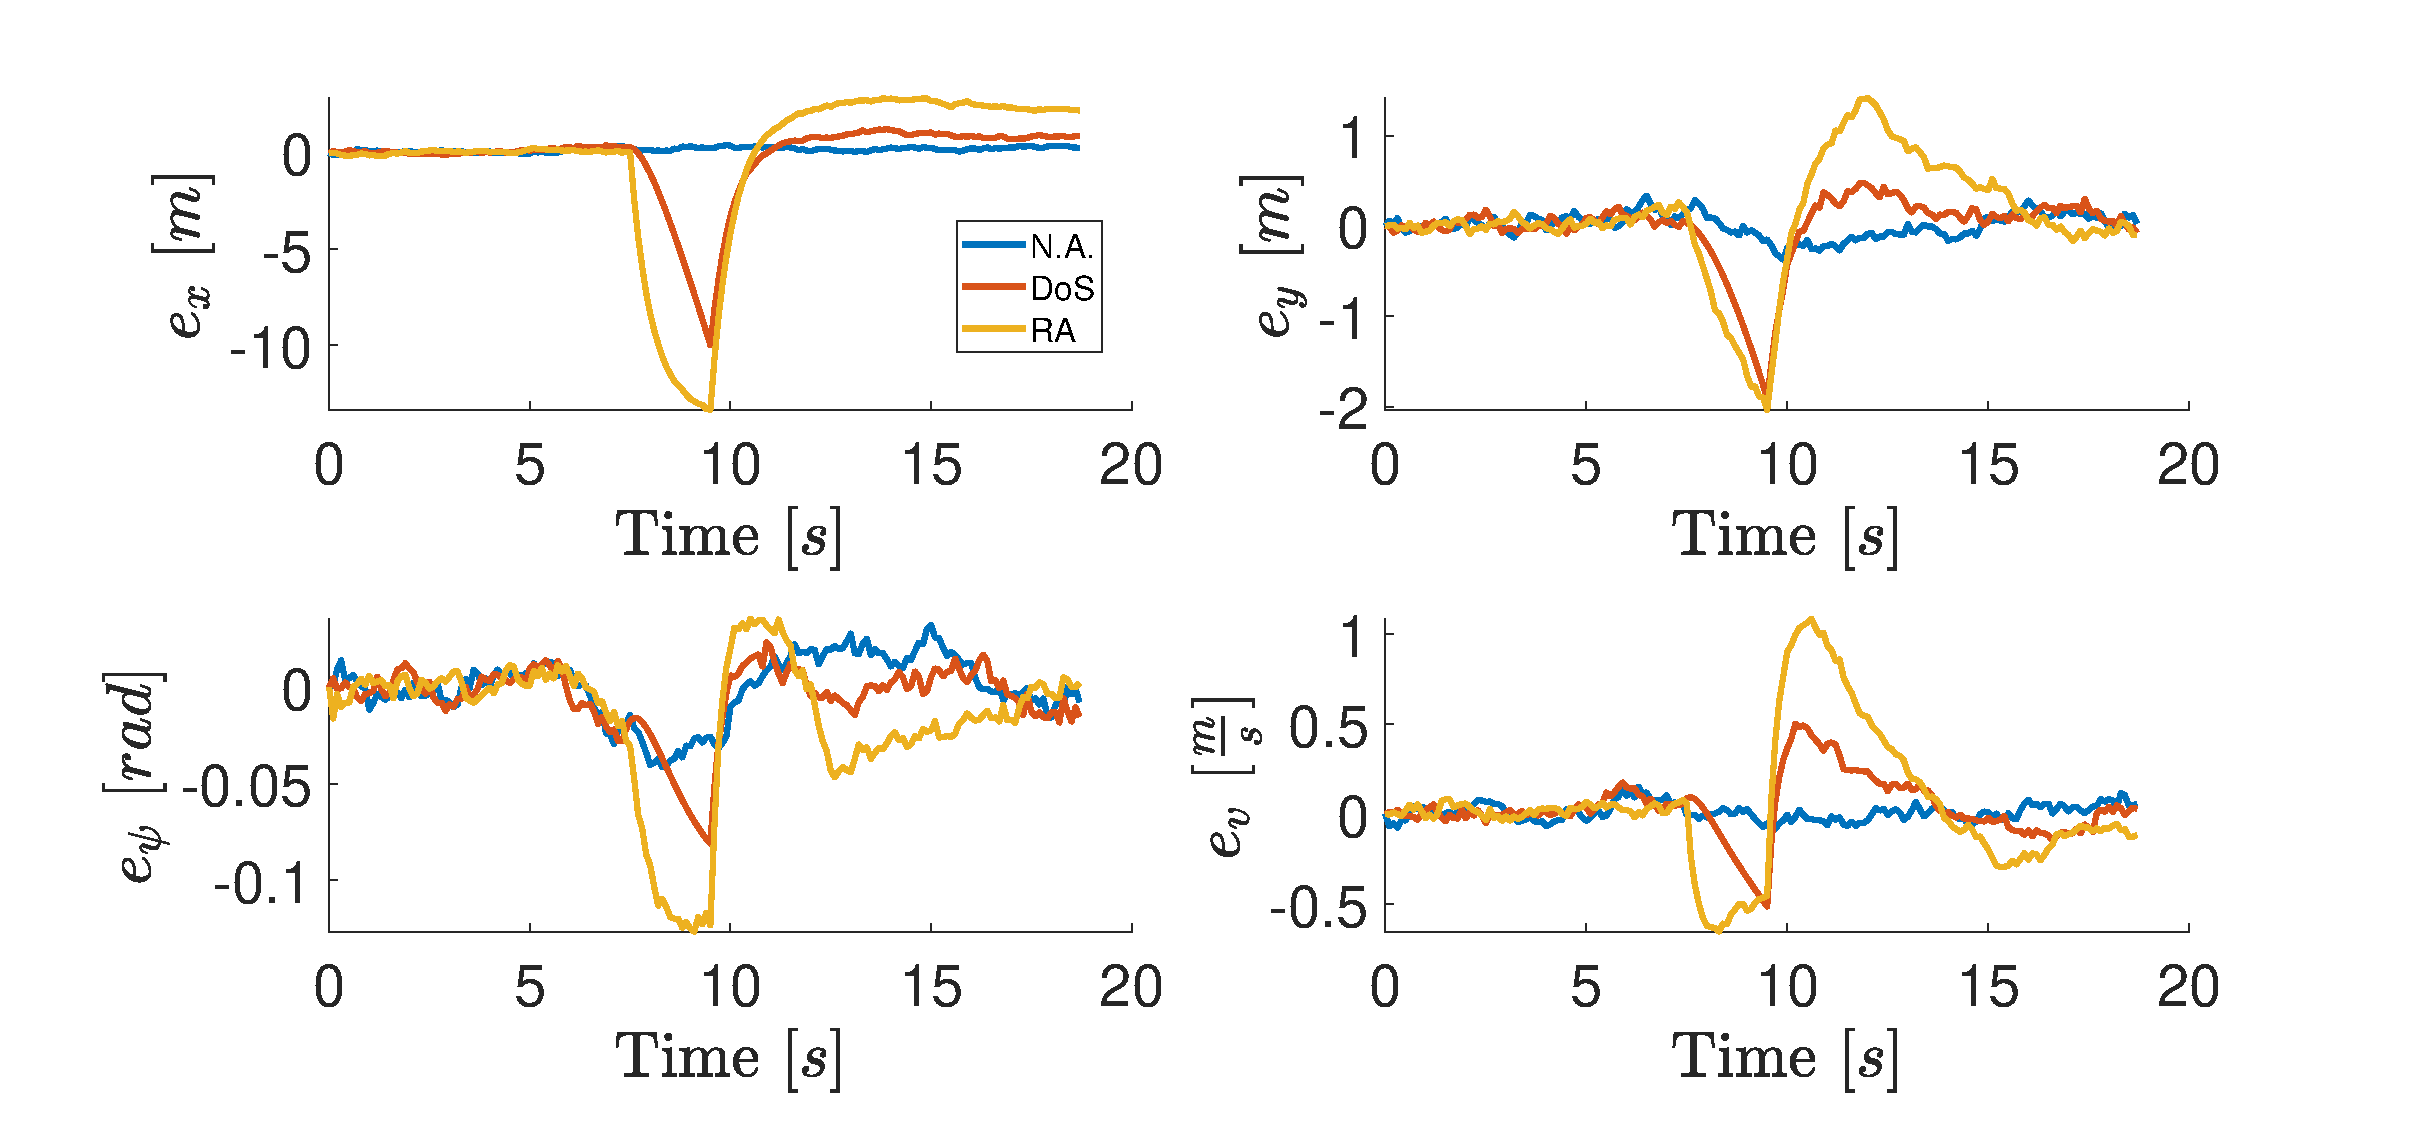
\includegraphics[scale=0.4]{figure/Part2/Chapter6/Figures/Errors_All.eps}
	\caption{Errors $e_{\zeta}$. Top-left: $e_x$. Top-right: $e_y$. Bottom-left: $e_{\psi}$. Bottom-right: $e_v$.  }
	\label{fig:gamma_error}
\end{figure}

\begin{figure}
	\centering
	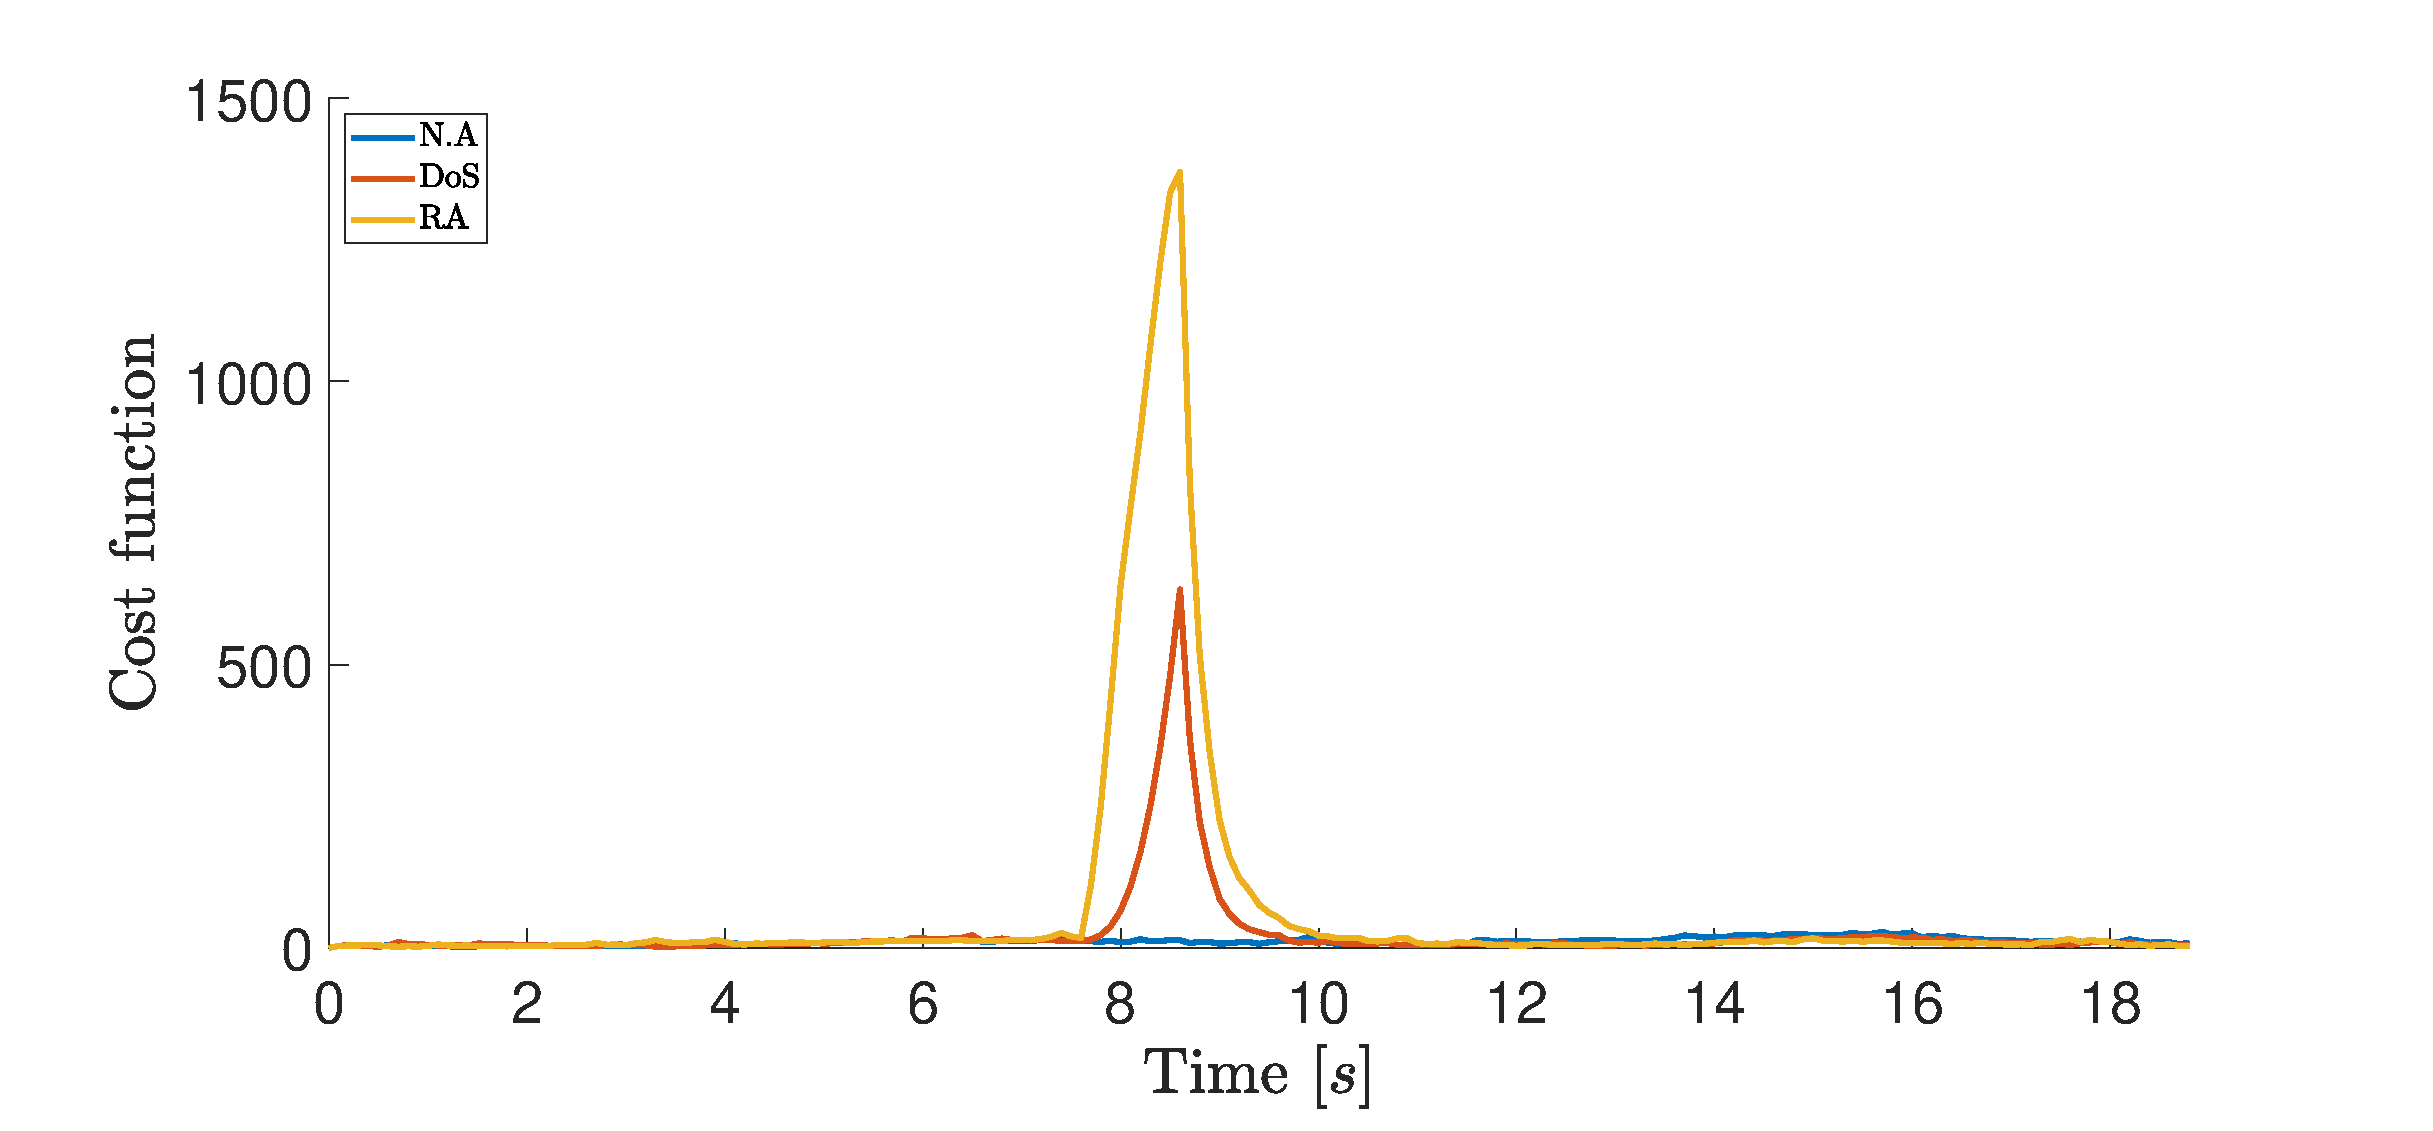
\includegraphics[scale=0.4]{figure/Part2/Chapter6/Figures/J_All.eps}
	\caption{Functional cost $J^\ast$. } 
	\label{fig:gamma_J}
\end{figure}

\begin{figure}
	\centering
	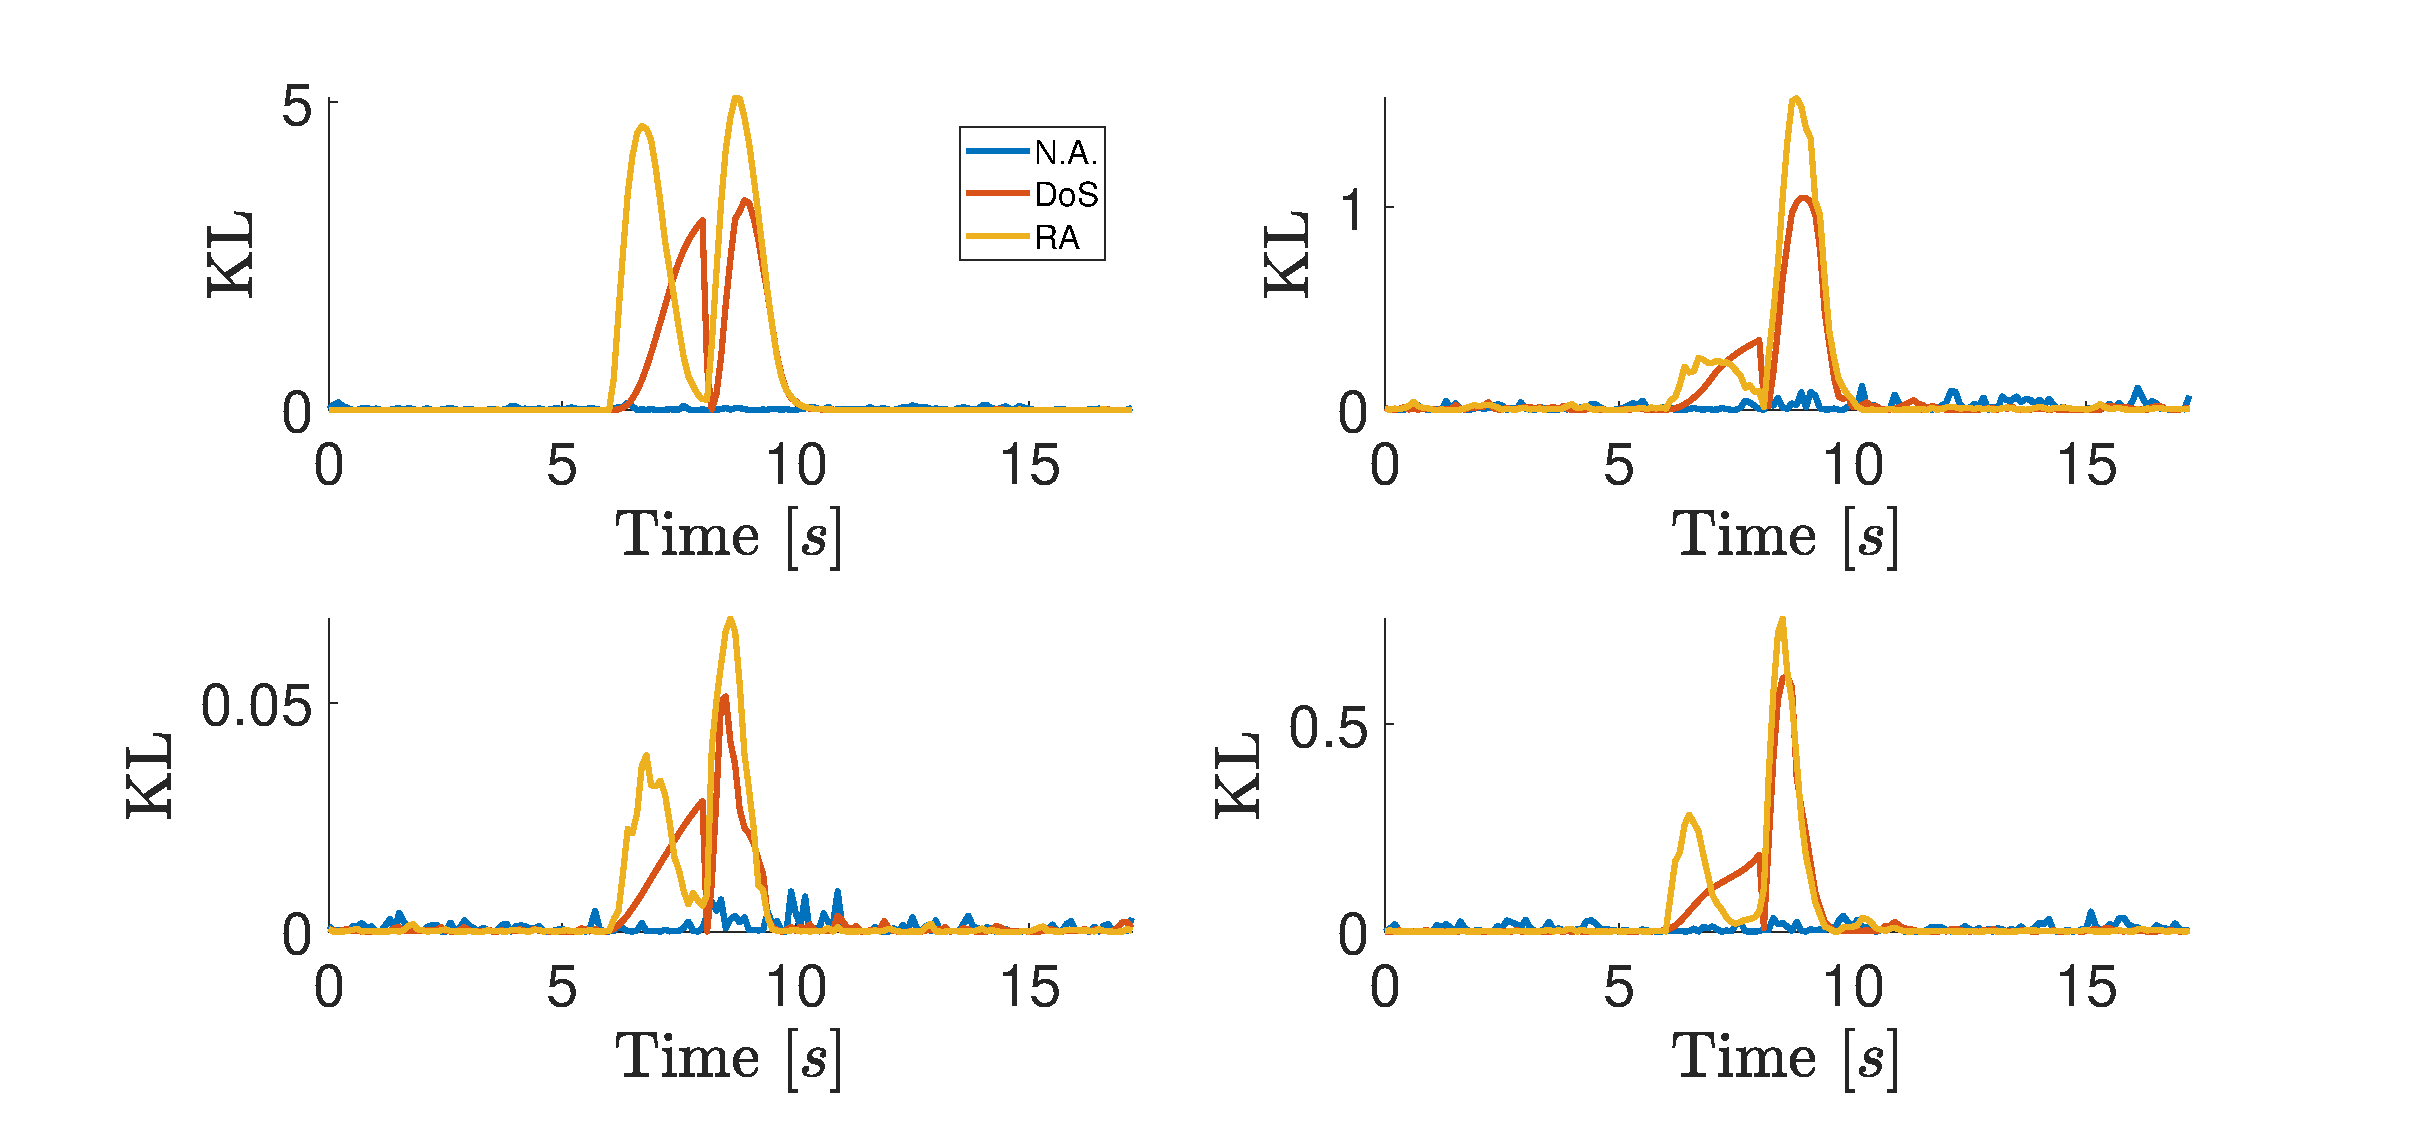
\includegraphics[scale=0.4]{figure/Part2/Chapter6/Figures/KL_All.eps}
	\caption{KL Divergences $D^{\mathrm{KL}}$. Top-left: $D^{\mathrm{KL}}\big(\bar{E}_x \| Q_x\big)$. Top-right: $D^{\mathrm{KL}}\big(\bar{E}_y \| Q_y\big)$. Bottom-left: $D^{\mathrm{KL}}\big(\bar{E}_\psi \| Q_\psi\big)$. Bottom-right: $D^{\mathrm{KL}}\big(\bar{E}_v \| Q_v\big)$. } 
	\label{fig:gamma_KL}
\end{figure}

\subsubsection{Classifier Training}
In order to build the attack dataset for the training of the detection model, for each class $N_{\rm sim}=10000$ simulations for the overtaking scenario have been carried out. Regarding the class~$0$, no attacks is injected all along the overtaking maneuver, whereas, regarding the other classes, the corresponding attack is injected. At the beginning of each attack,~$t_a$ and~$T_d$ are computed as realization of uniformly distributed random variables with supports~$\big[t^-_a, t^+_a\big]\subset\mathbb R^+$ and~$\big[T^-_d, T^+_d\big]\subset\mathbb R^+$, respectively. The features~\eqref{eq:J},~\eqref{eq:err} and \eqref{eq:kl_div} of the classes $1$-$6$ are collected during the attack phase \mbox{$t \in \big[t_a,t_a+ T_d\big]$}, while for the class $0$ the same features are collected during the whole time of the simulation.



The number of instances of each class during the training is reported in Table~\ref{table:classes}. In particular, the dataset is built such that in half of the instances there is an attack while no attacks are taking place in the rest.

The features $e_{\zeta}$, $J$ and $D^{\mathrm{KL}}$ during the training are reported respectively in Fig.~\ref{fig:gamma_error}--\ref{fig:gamma_KL}, where the Yellow lines refer to \gls{ra}, the Orange lines refer to DoS attacks and the Blue lines refer to no attacks (N.A.).

The confusion matrix of the \gls{csvm} Classifier is reported in Fig. \ref{fig:Confusion_matrix}, and Precision, Recall and F1 Score are reported in Table \ref{table:Best_classifier}.
%
\begin{figure}[h]
	\centering
	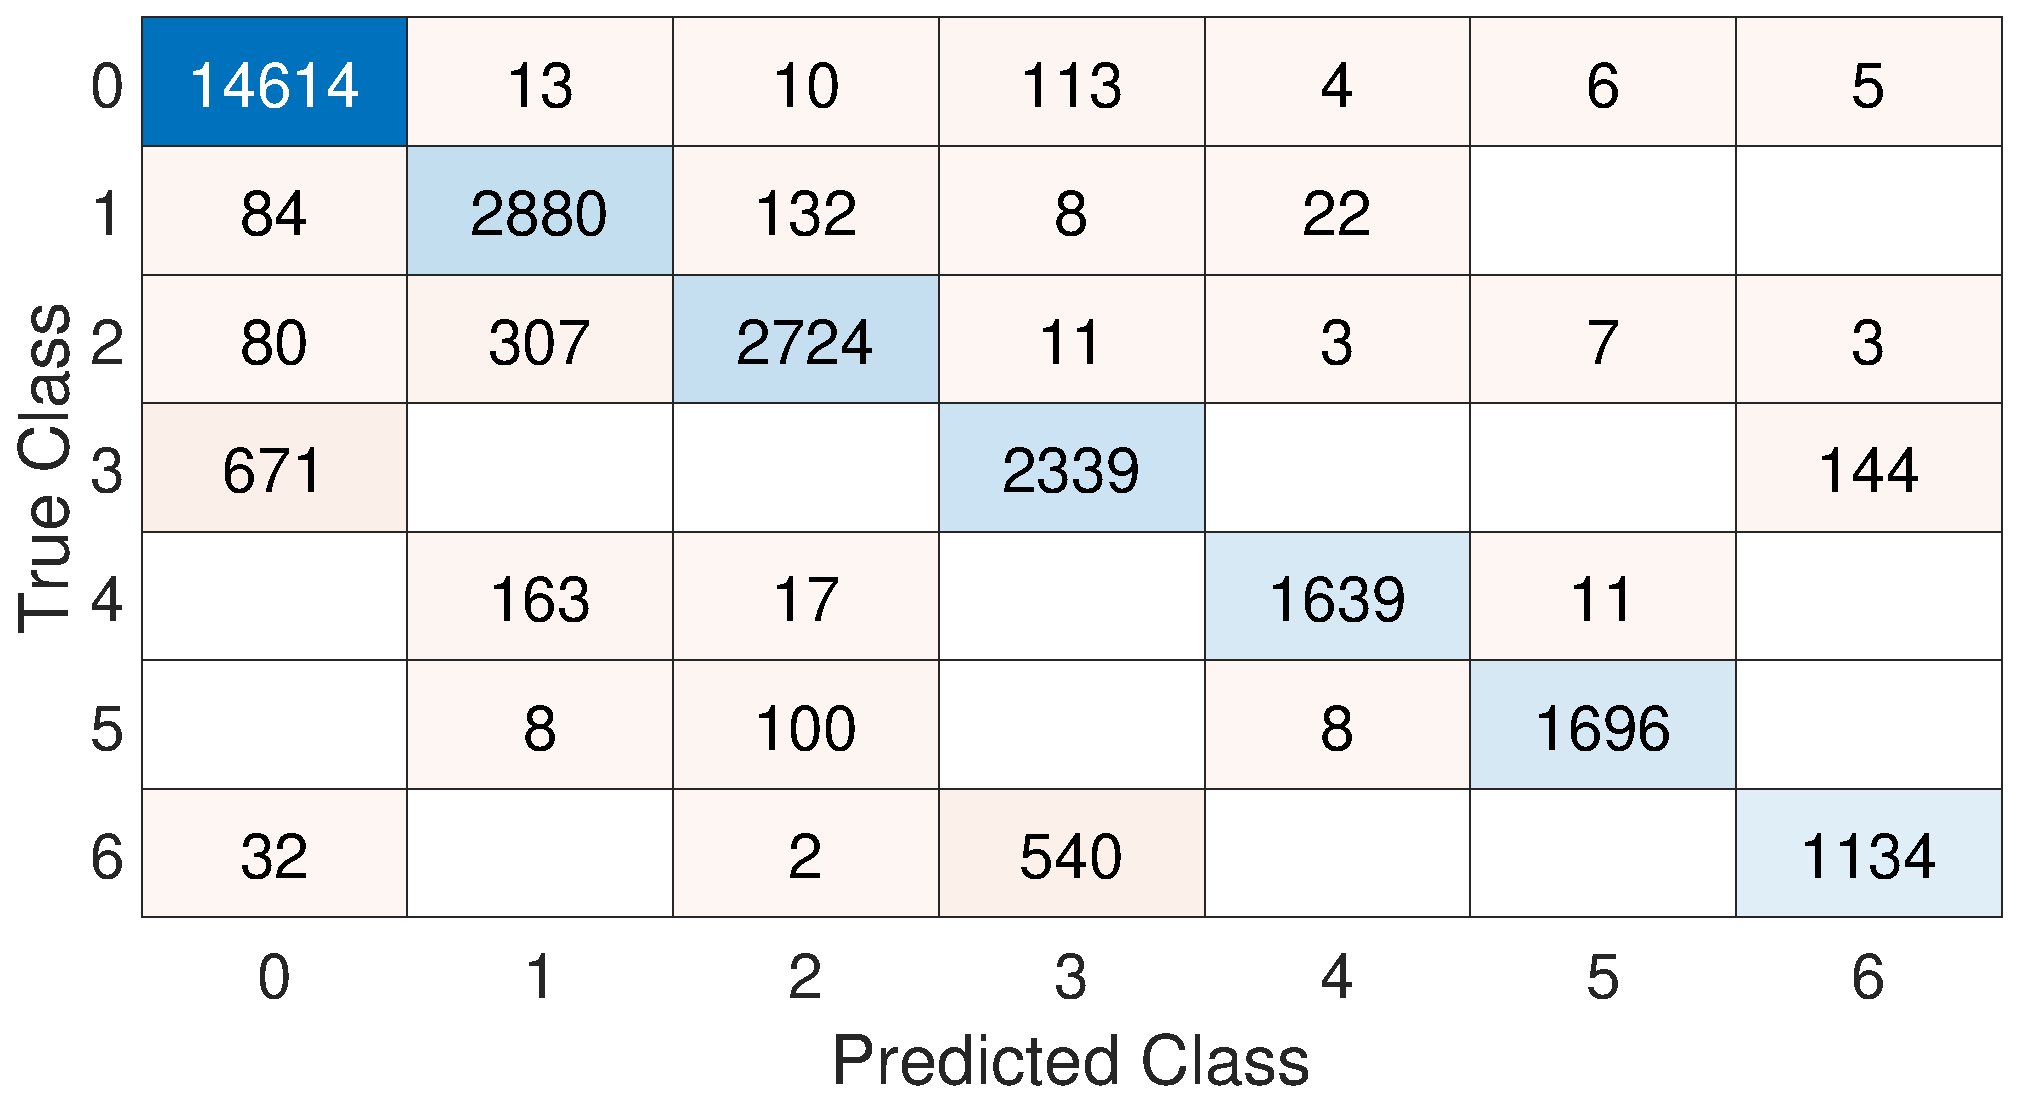
\includegraphics[scale=0.35]{figure/Part2/Chapter6/Figures/Confusion_matrix.eps}
	\caption{\gls{csvm} Confusion Matrix. }
	\label{fig:Confusion_matrix}
\end{figure}
%
%
%
%
In order to understand the effectiveness of the proposed approach we carried out a confrontation with the \gls{ra} Detector proposed in~\cite{detection_1} whose Precision, Recall and F1-Score result to be $81.6\%$, $35.1\%$ and $49.0\%$, respectively. While the proposed approach achieves Precision of $98.9\%$, Recall of $94.4\%$ and F1-Score of $96.6\%$. As it is possible to see, the obtained results show that the predictive features of the \gls{nmpc} could obtain satisfactory Classifier metrics. Regarding the metrics shown in Table~\ref{table:Best_classifier}, we remark that classes $2$ is less detectable compared to class $3$ and class $5$ is less detectable respect to class $6$, due to the different impact that the corresponding type of attack has on the performances of the control architecture.  
%
\begin{table}[h]
	\centering
	\begin{tabular}{ |c|c|c|c| } 
		\hline
		Classes  & Precision & Recall & F1 Score\\
		\hline
		\multirow{6}{2em}{\centering 0\\ 1\\ 2\\ 3\\ 4\\ 5\\ 6\\ } 
		& $94.4 \, \%$ & $99.0 \, \%$ & $ 0.96 $\\  
		& $85.4 \, \%$ & $92.1 \, \%$& $ 0.88 $ \\
		& $77.7 \, \%$ & $74.2 \, \%$& $ 0.75 $ \\
		& $91.3 \, \%$ & $86.9 \, \%$& $  0.89 $ \\ 
		& $97.8 \, \%$ & $89.6 \, \%$& $ 0.93 $ \\ 
		& $88.2 \, \%$ & $66.4 \, \%$& $ 0.75 $ \\ 
		& $98.6 \, \%$ & $93.6 \, \%$& $0.96 $ \\ 
		\hline
	\end{tabular}
	\vspace{0.25 cm}
	\caption{Cubic SVM Classifier.}
	\label{table:Best_classifier}
\end{table}
%%% END SECTION ============================================================

%%% START SECTION ==========================================================

\section{Simulations and results}
\label{sec:fourth}
%
In this section we present the simulation outcomes of the proposed scheme in comparison with those of a \gls{av} architecture where no mitigation is considered. The software is implemented in MATLAB\textsuperscript{\textregistered} and CasADi~\cite{Casadi}, and the simulation parameters are reported in Table~\ref{tab:parameters}.
%
\begin{table}[ht]
	\centering
	\begin{tabular}[ht]{|l|l|c|}
		\hline
		\textbf{Parameters} & \textbf{Value}\\
		\hline
		$l_f$& \SI{1.738}{\metre}\\
		$l_r$& \SI{1.105}{\metre}\\
		$T_s$& \SI{0.1}{\second}\\
		$S$&  $\mathrm{diag}\big(100,1000\big)$ \\
		$R$& $\mathrm{diag}\big(0.1,0.1\big)$\\
		$L$& $\mathrm{diag}\big(10,10,400,200\big)$ \\
		$\dot{u}_{{\rm max}}$& $\begin{bmatrix}\SI{0.6}{{\metre}/{\second^3}} & \SI{0.2}{{\radian}/{\second}}\end{bmatrix}^\top$ \\
		$\dot{u}_{{ \rm min}}$& $\begin{bmatrix}\SI{-0.6}{{\metre}/{\second^3}} & \SI{-0.2}{{\radian}/{\second}}\end{bmatrix}^\top$ \\
		${u}_{{ \rm max}}$&$\begin{bmatrix}\SI{2.5}{{\metre}/{\second^2}} & \SI{0.7}{\radian}\end{bmatrix}^\top$\\
		${u}_{{ \rm min}}$& $\begin{bmatrix}\SI{-2.5}{{\metre}/{\second^2}} & \SI{-0.7}{\radian}\end{bmatrix}^\top$ \\
		$H_p$& 30 \\
		$N_M$& 15 \\
		\hline
	\end{tabular}
	\caption{Parameter values.}
	\label{tab:parameters}
\end{table}%
%
%	 
In \mbox{Fig.~\ref{fig:no_attack}-\ref{fig:MPC_dos}}, the simulations regarding the overtaking maneuver are reported in case no mitigation countermeasure is implemented. Cyan lines refer to the trajectory references, orange lines refer to the state measurements and Yellow lines refer to the state estimates. Only attacks on the entire attack space have been considered with $t_a= \SI{9.5}{\second}$ and $T_d=\SI{2}{\second}$ for \glspl{ra} and $t_a= \SI{7.5}{\second}$ and $T_d=\SI{2}{\second}$ for \gls{dos} attacks. For different values of $t_a \in \big[t^-_a, t^+_a\big]$ the Detector behaviour is the same. 

In Figs.~\ref{fig:MPC_RA},~\ref{fig:MPC_dos} it is possible to note that  the error between the measured/actual $x$ and $y$ and the reference in \glspl{ra} is greater than in \gls{dos} attacks, thus implying a higher control degradation. This happens because in \gls{dos} attacks only the state in the last sampling interval is available while in \glspl{ra} a replayed state sequence is available that is related to a time window spanning several samples back in time. Reintroduce these past state estimate sequence to the \gls{nmpc} produces a considerable error in the calculation of the control inputs; 
in particular, the greater the replay time, the more evident the degradation of performance is.

The effectiveness of the \gls{imps} architecture is shown in \mbox{Fig.~\ref{fig:Simulation_Mitigator}} where the heading angle, the velocity and the position are reported when an \gls{ra} with  $t_a= \SI{10}{\second}$ and $T_d=\SI{2}{\second}$. As it is possible to notice, the implemented \gls{imps} is able to detect in time the cyber-attack and the mitigation action allows the \gls{av} to conduct an overtaking maneuver safely. Indeed, the safety of the maneuver is obtained by minimizing the position error with respect to the trajectory planned by the planner. Furthermore, the time to detect the attacks is of two time steps.

The effectiveness of proposed architecture is also highlighted in Fig.~\ref{fig:Safe_set} which reports the trajectories in the $e_x-e_y$ plane for an AV during overtaking when both the proposed scheme is implemented and the proposed scheme is not implemented. An ellipsoidal safe region for the overtaking maneuver is also plotted (solid red line) and the trajectory position errors are reported for the aforementioned simulations. The safe region is computed as the maximum deviation with respect to the trajectory reference which allows the \gls{av} to perform the overtaking maneuver without damaging or hitting possible obstacles.

Cyan, Magenta, Green and Blue represent the simulations regarding No Attack, \gls{ra} with \gls{imps}, \gls{dos} attack and \gls{ra} without \gls{imps}, respectively. The novel \gls{imps} implemented allows to reduce the effect of cyber-attacks generated by a hacker. In cases of no detection and mitigation of \gls{ra} and \gls{dos} attack, the errors of the trajectory result out of the safety region, which could cause damages and possible injuries to the driver.
%
\begin{figure}
	\centering
	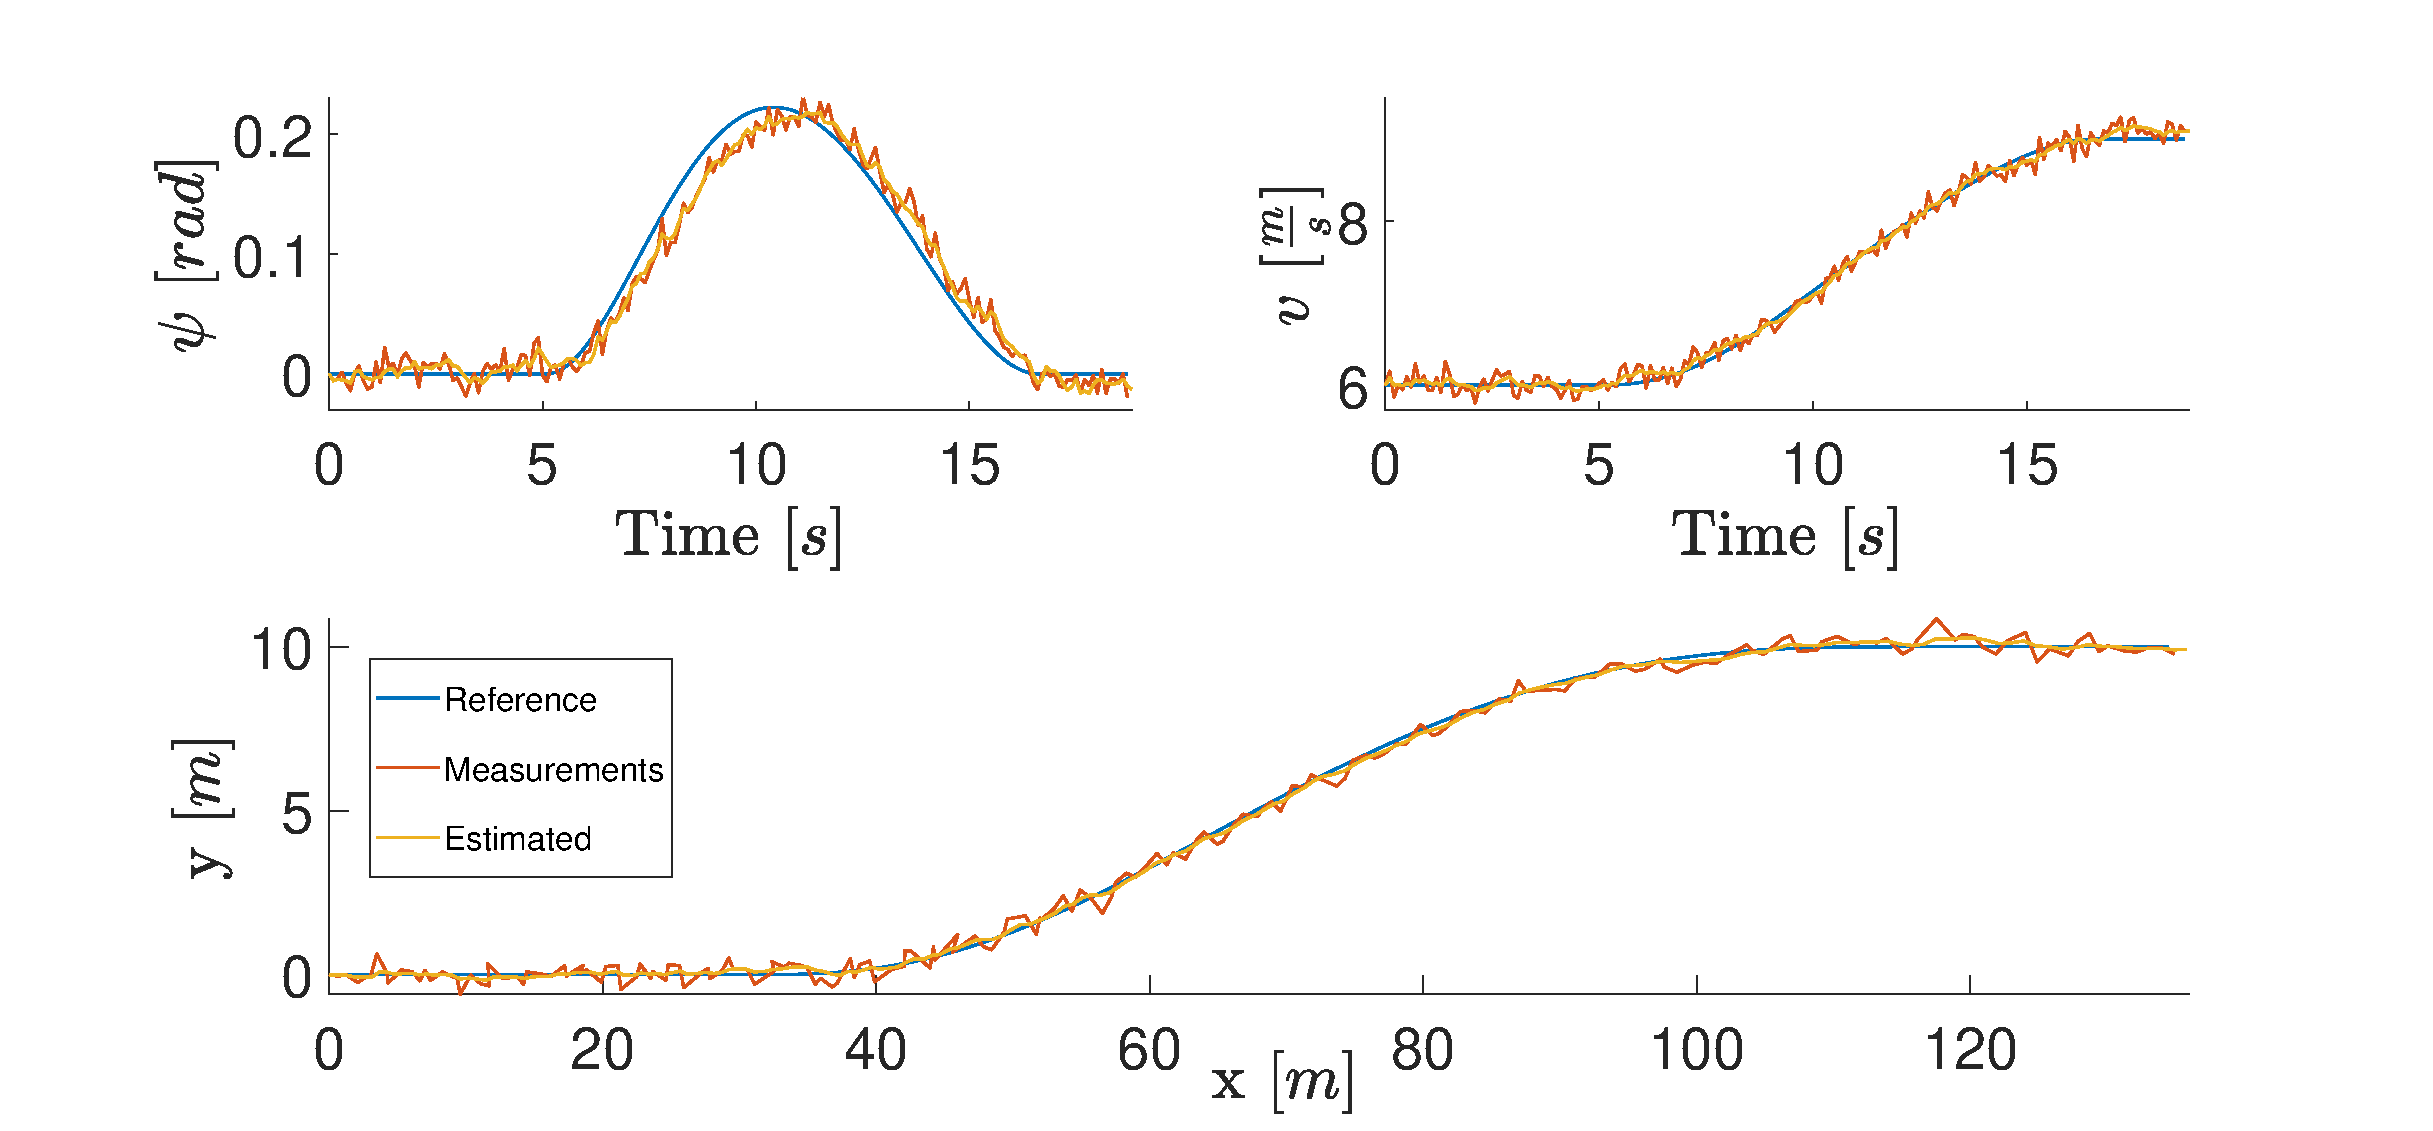
\includegraphics[scale=0.4]{figure/Part2/Chapter6/Figures/MPC.eps}
	\caption{No attacks.}
	\label{fig:no_attack}
\end{figure}
%
\begin{figure}
	\centering
	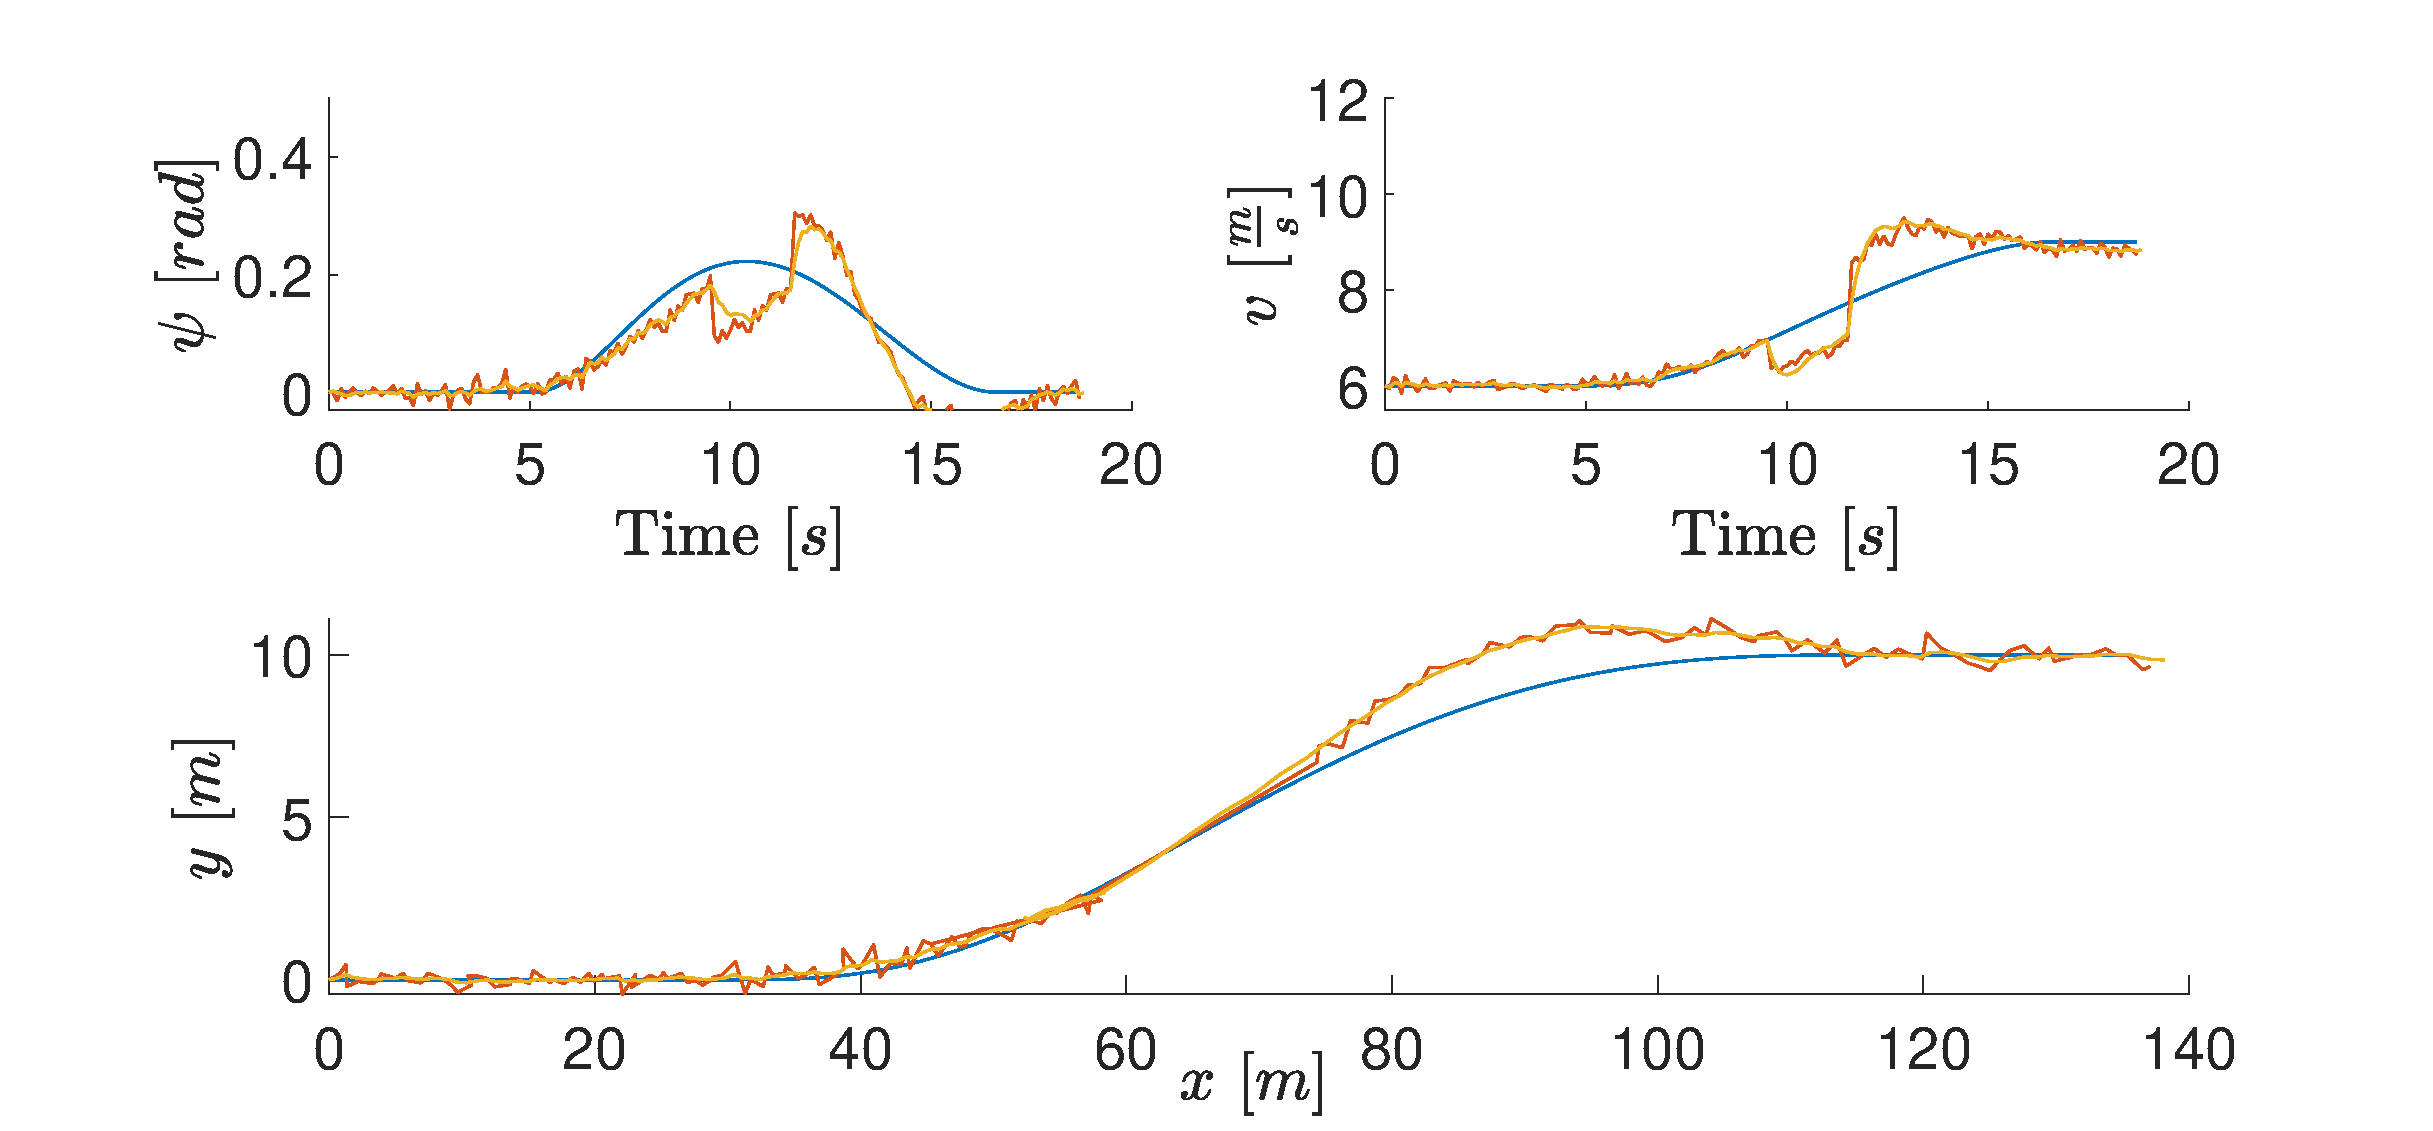
\includegraphics[scale=0.4]{figure/Part2/Chapter6/Figures/MPC_Replay.eps}
	\caption{\gls{ra}.}
	\label{fig:MPC_RA}
\end{figure}
%
\begin{figure}
	\centering
	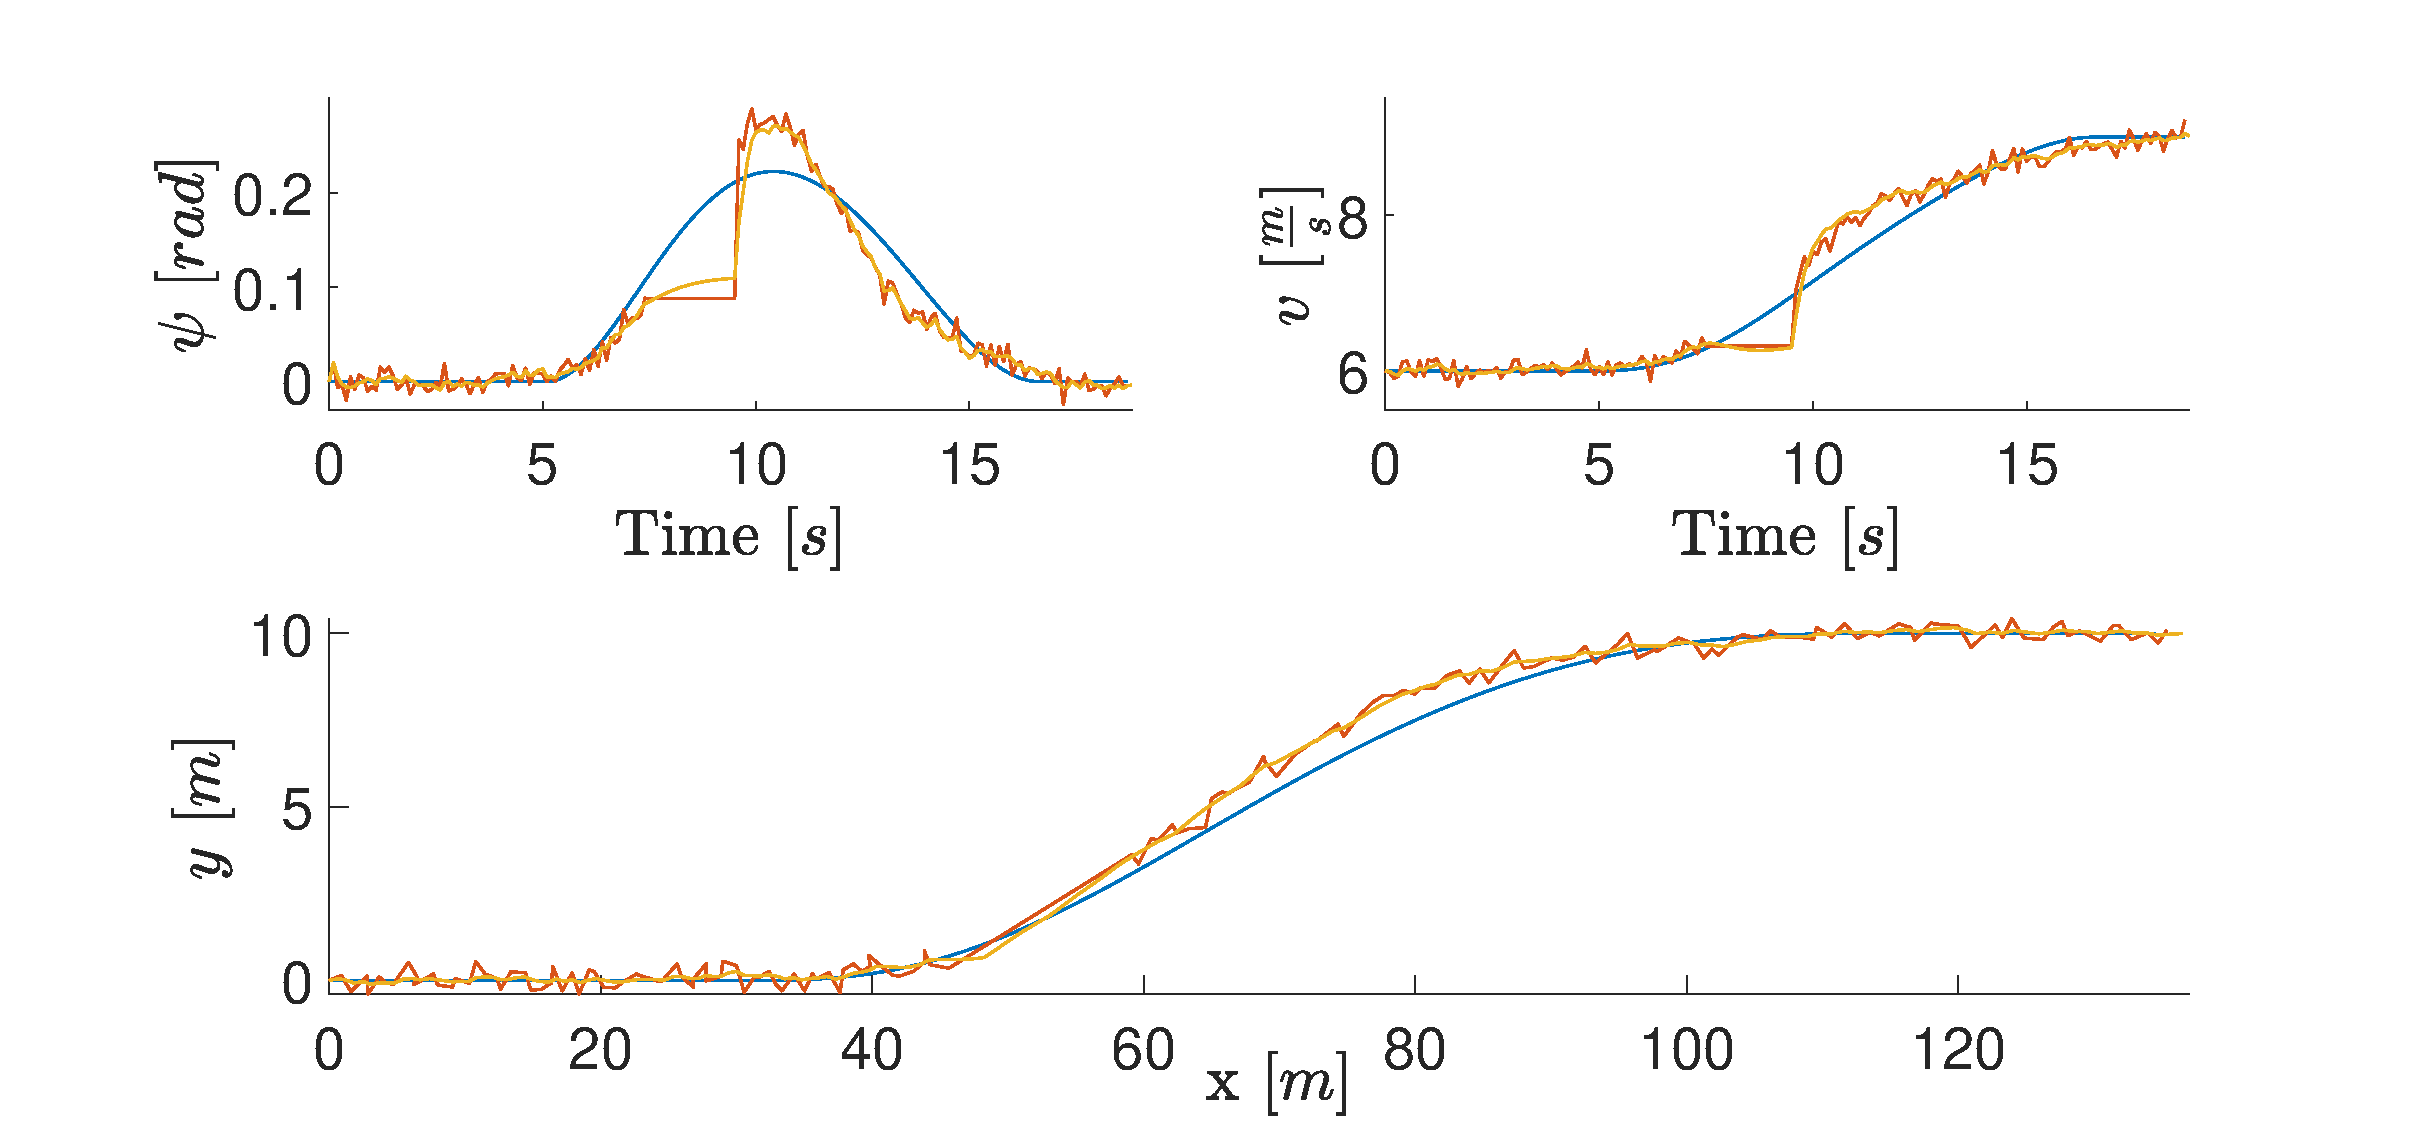
\includegraphics[scale=0.4]{figure/Part2/Chapter6/Figures/MPC_DoS.eps}
	\caption{\gls{dos} attack.}
	\label{fig:MPC_dos}
\end{figure}

%


\begin{figure}
	\centering
	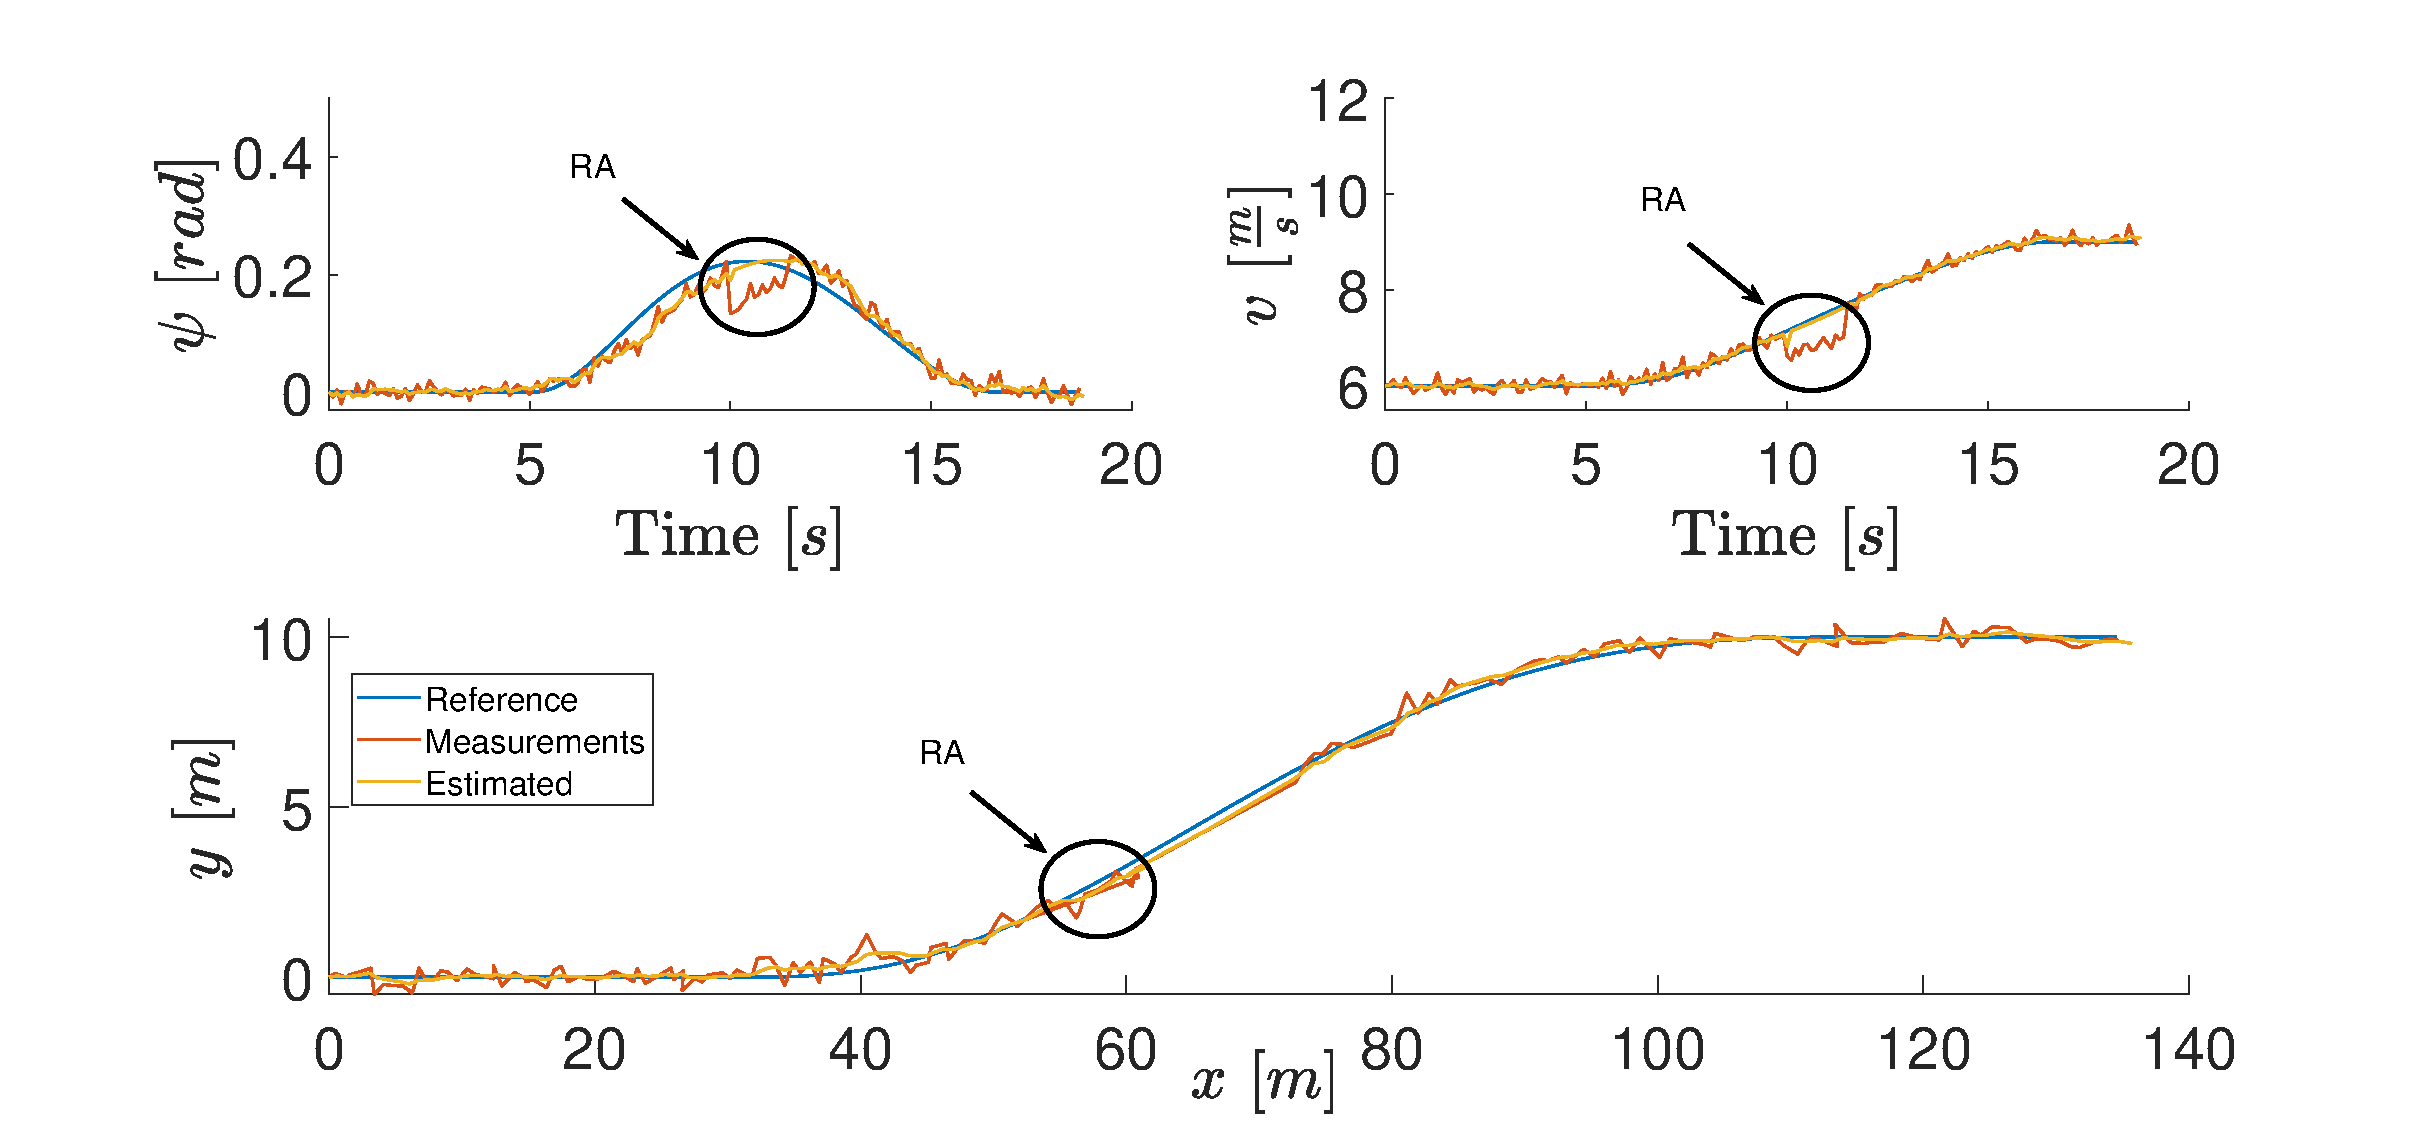
\includegraphics[scale=0.4]{figure/Part2/Chapter6/Figures/Mitigation_fin.eps}
	\caption{\gls{ra} mitigation using \gls{imps}. Start time attack and duration are  $t_a= \SI{10}{\second}$ and $T_d=\SI{2}{\second}$, respectively. Top-left: Heading angle. Top-right: Velocity. Bottom: Position.   }
	\label{fig:Simulation_Mitigator}
\end{figure}
%
\begin{figure}
	\centering
	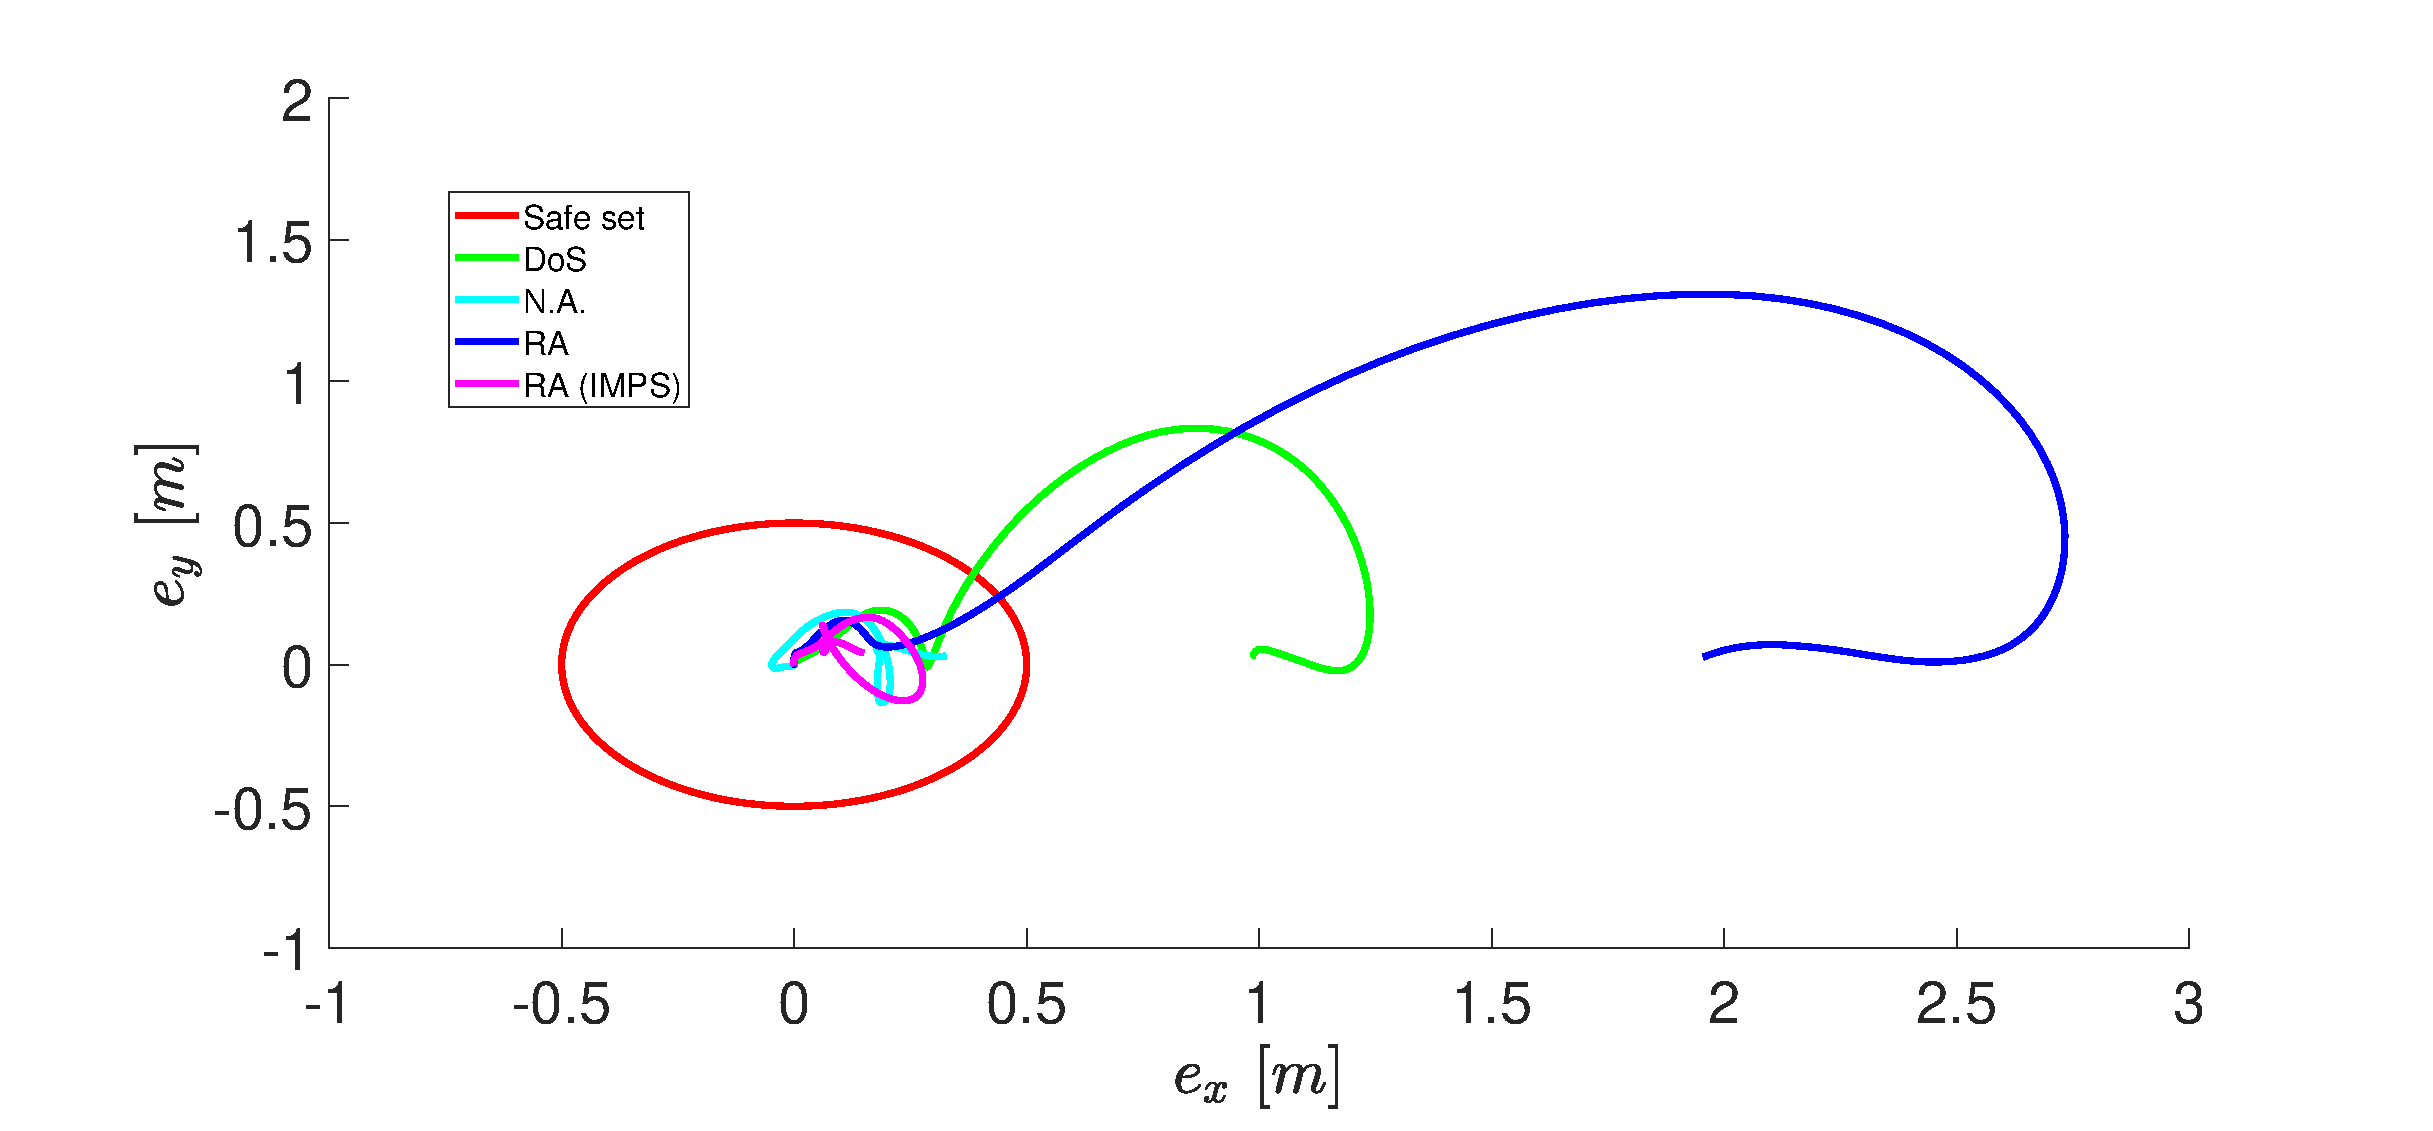
\includegraphics[scale=0.4]{figure/Part2/Chapter6/Figures/Safe_set.eps}
	\caption{Safe region and error trajectories. }
	\label{fig:Safe_set}
\end{figure}
%




\clearpage
\section{Chapter Summary}


The conclusion of this chapter highlights the Informative Model Predictive Scheme algorithm's successful application in enhancing cybersecurity for autonomous vehicle systems, particularly during overtaking maneuvers vulnerable to cyber-attacks such as Replay Attacks and Denial of Service. Numerical results from simulations validate the efficacy of the I-MPS, demonstrating its potential in accurately detecting and mitigating cyber threats in real-time. These findings suggest a significant step forward in vehicular cybersecurity, illustrating the innovative synergy between machine learning algorithms and control systems in combatting cyberattacks. The results also indicate areas for further accuracy enhancement, reinforcing the I-MPS as a pioneering approach in the ongoing evolution of cybersecurity measures for autonomous vehicles.

\part{COOPERATION}
\label{part:3}
\input{part3}


%\part{Process Monitoring and Learning}

%\lhead{\bfseries MONITORING AND LEARNING}
\chapter{Learning-based anomaly detection for steel-making plant }
\label{Chapter:5}
In this Chapter we propose a FDD method leveraging on class-support One-class Support vector machine (OC-SVM)-based technique; the  model is able to discriminate between normal and anomalous operating conditions indicative of an incoming breakdown in a production context where faults are extremely rare. In fact, the OC-SVM method~\cite{scholkopf2001estimating, acernese2019_ECC} relies on the assumption that the entire training sample of the model belongs to the nominal (safe) operating conditions of the production process. However, when the training data set is affected by a significant subsample  of  non-nominal operating conditions, the OC-SVM exhibits weaknesses. For this reason, we combine the OC-SVM with some preparatory steps aiming to maximize performance. Namely, we adopt a PCA as a feature extraction process, and a Gaussian Mixture Model (GMM) technique \LR{for training set selection} %as a clusterization tool  
ensuring a  sufficiently homogeneous yet informative training data set.\\
% Both techniques essentially rely on the fusion of information received from sensors placed along the production process; we obtained one reliable classification criterion to robustly identify anomalous, normal, and intermediate operating conditions. Note that in the sequel, we will refer to anomaly and outlier interchangeably.
\indent Moreover, we compare the performance with a multivariate statistical methodology recently developed for this particular application~\cite{sarda2021}. 
% the method aims to detect anomalous data revealing  an incipient failure or a degradation of process' performances~\cite{sarda2021} in a steel plant. 
This method incorporates two techniques: %a preliminary fault detection is  carried out based on a straightforward and computationally mild static analysis of the available data. Secondly, a  more complex and computationally intensive method is performed, targeting a precise identification of the anomalies based on the dependencies on time of system's conditions and on the outcomes of the first step. More precisely 
a preliminary anomaly detection technique that uses the reweighted minimum covariance determinant (RMCD) estimator is
%It relies on the nature of anomalies  -  outliers in statistical jargon  -i.e., measurements aside from main features of most of the data,  exhibiting their own pattern or even no pattern at all. In fact, the robust distance fuses the information received from sensors displaced on the production process, hence obtaining one reliable measure and the corresponding trade off, easily implementable and adaptable to all process stages. \\
combined with the hidden Markov model (HMM) theory to obtain a robust FD and diagnosis methodology, able to take into account also the time-varying nature of the data.\\
% . More precisely, the HMM is fitted over the distances of the data points from the robust fit stemming from RMCD estimation; this enables the implementation of a dynamic anomaly detection strategy which takes into account the time-varying nature of the data and infers hidden states in the production process along with their state transition probabilities which model the probability of moving towards degradation stages of the production equipment to the final inferred state, denoting a failure.
%The method we developed is a first attempt to overcome the absence of data on faults events. Robust distances are the key element since outliers can only be properly detected  measuring the distance of data points from a robust fit. To this end, 
\indent Among our main contributions we consider: (i) an automatic FD and diagnosis procedure to detect anomalies in large data sets with strongly unbalanced clusters; (ii) the extension of the standard anomaly detection methods to an OC-SVM-based method that provides additional information about the anomaly severity; (iii) the comparison of the OC-SVM-based method with a validated HMM-based method, considering different training sets with different associated operating conditions, in order to highlight the advantages and drawbacks of both methodologies.
The method is tested on data  generated from the rolling mills of the steel production plant Pittini's group, located in the South of Italy.

% We applied both methods (OC-SVM-based and HMM-based) to the available process data of an hot rolling mill line placed in a steel making plant. We considered different training sets with different associated operating conditions, in order to highlight the advantages and drawbacks of both methodologies.

%Frequency domain analysis is most frequently adopted in anomaly detection of rotating machines since the direct correspondences between specific faults and their characteristic frequencies is a priori known (Randall, 2011). This motivates the frequency-domain procedure to identify anomalies behaviour in process parameters, at least those anomalies related to rotating mechanical parts.  Notice that standard spectral analysis is not particularly effective in this case, since the amplitude of the impulsive type signals associated to defects of the bearings is typically much smaller than that of the signal measured in the absence of fault. Thus, it becomes necessary to employ specific frequency domain techniques that enable to discriminate the contributions associated to faults from the characteristic frequencies of the system in the spectra of the vibration signal. For this purpose, one can resort to the envelope analysis, a well-established technique, see Randall and Antoni (XXXREFFF), widely employed in the diagnosis of rotating machines. This analysis requires first that the data be appropriately filtered to emphasize the fault with respect to other components, so as to facilitate the fault detection. The design of such filter is here based on the analysis of the spectral kurtosis (XXXREF).  Since this procedure is computationally much more intensive than the previous one based on multivariate analysis, it provides a complementary tool, which can be employed when the former suggests the possibility of a fault, with the aim of providing further evidence and details on the fault.

%\LR{\AAC{MOVE TO THE INTRODUCTION???} In the context of supervised learning SVM is an established model for data classification and regression [REFXX]. The SVM model generates nonlinear decision boundaries between classes finding linear boundaries in transformed higher dimensional feature space obtained with kernels. The criteria is to choose boundaries such that the margin between data belonging to different classes is maximum while ensuring a good classification.}
\section{Proposed fault detection and diagnosis procedure}\label{sec:methodology}
\LR{In this section it is reported the description of the novel OC-SVM based method for condition monitoring.The method is general and can be applied in different manufacturing contexts in which fault data are rare or missing. First we describe the feature transformation process using PCA giving a brief description of this technique that is also useful for a better  comprehension of the successive steps. Then we introduce GMM salient features and how it can be conveniently use to split data-set into test and training set for OC-SVM. Finally we describe OC-SVM, its ability to discriminate between nominal and anomalous operating conditions given a proper choice of charateristic parameters and its fitting to condition monitoring.}
%In this section we describe a condition monitoring procedure to automatically detect anomalies. The procedure is broad and may be applied to several manufacturing context; in the subsequent section we show how we successfully applied it to a  hot rolling mill lines of steel making plants. We show how the PCA can be cast in the feature extraction process, and how the GMM technique can be used as a tool ensuring a sufficiently homogeneous yet informative training data set. We further introduce the optimization problem representing the OC-SVM method and its ability in \LR{between nominal and anomalous operating conditions }%identifying clusters
%in unlabeled data sets.

\textbf{Notation.} We denote by $\mathbb{R}$ and $\mathbb{N_{+}}$ the sets of real and positive natural numbers, respectively. Uppercase bold variables denote matrices, lowercase bold ones represent vectors, assumed to be column, i.e., $\mathbf{x}=(\cdot,\dots,\cdot)$ is a column vector.

\subsection{Features transformation process}
\LR{Dimensionality reduction is a fundamental step in many machine learning algorithms. In fact high dimensional data sets often include non relevant attributes that might not affect the output of the prediction. PCA is a useful statistical tool that provides a data driven coordinate system to represent high dimensional correlated data in low dimensional space of uncorrelated dimensions, preserving most of the variance of the original data.  This makes data handier, and significantly reduces the computational load associated with the execution of machine learning algorithms on high dimensional data \cite{brunton2019data}\cite{Reddy}.}
\review{
Let $\mathbf{O(t)}=(\mathbf{o}_1(t),\mathbf{o}_2(t),\dots, \mathbf{o}_n(t))^{\top}$, be a collection of random processes(representing the outcome of the sensors installed into the plant) such that for fixed time $t^*$, the generic $\mathbf{o_i(t^*)}$ is a random variable from normal distribution $\mathcal{O}\sim \mathcal{N}(\mathbf{\mu_i},\mathbf{\sigma_i})$, where $\mathbf{\mu_i}$ is the mean , $\mathbf{\sigma_i}$ is the variance. Assume that each process is sampled with fixed step $T_S$ over a predefined time interval $T$ such that we can construct the  sample $\mathbf{O}=(\mathbf{o}_1,\mathbf{o}_2,\dots, \mathbf{o}_n)^{\top}$  where $\mathbf{o}_{i}=(o_{i1},o_{i2},\dots, o_{ip})\in \mathbb{R}^{p}$,and $p\in \mathbb{N}^+$ is obtained as $\frac{T}{T_S}$.
One may extract from each sample   $\mathbf{O}$ a fixed number $N$ of time-series of length $\omega$ --- eventually allowing some overlapping between the windows --- and compute some parameters (also called indices) over the windows for each sensor.  We refer to the output of this stage as the data set of the parameters, i.e., $\mathbf{Z} = (\mathbf{z}_1,\mathbf{z}_2,\dots, \mathbf{z}_n)^{\top} \in \mathbb{R}^{n \times (Nm)}$, with $m$ the number of extracted parameters.}

Table~\ref{tab: parameters} shows the list of parameters extracted in the case study described in this paper. They include mainly time-domain statistical indices, and time-frequency domain parameters from the signal processing theory. For an overview on the definition of these indices and their properties see~\cite{acernese2020_JQME} and references therein. 
% Note that we limited the extraction some parameters to the vibration signals, because their sampling frequencies are very high w.r.t. other sensors and might provide useful information with these parameters.

 Considering the different nature of the measurement $\mathbf{Z}$ is normalized through min-max normalization and then the PCA is applied to generate the final set of features. Namely, for each $\mathbf{z}_j$, compute $\hat{\mu}_{j}=\frac{1}{N} \sum_{i=1}^{N} z_{i j}$, $j=1,\dots, m$ and the sample covariance matrix $\hat{\mathbf{\Sigma}}$ as:
\begin{equation}
    \label{eqn: covMat}
    \hat{\mathbf{\Sigma}}=\frac{1}{N-1}(\mathbf{Z}-\mathbf{M})^{\top}(\mathbf{Z}-\mathbf{M}),
\end{equation}
where $\mathbf{M} = \mathbb{1}_{N}~(\hat{\mu}_1, \dots, \hat{\mu}_m)$ is the sample mean matrix, and $\mathbb{1}_N$ is the identity $N$-vector. The eigenvectors are called principal components (PCs), and they can be ordered according to the ordered rank of the corresponding eigenvalues of $\hat{\mathbf{\Sigma}}$, from the highest to the lowest. The projection of the original parameters in the $k$-dimensional subspace, comprising of the first $k$ eigenvectors $\mathbf{e}_{1}, \ldots, \mathbf{e}_{k}$, is obtained as follows:
% and are associated with the highest variance direction in the feature space.
\begin{equation}
    \label{eqn: pca}
    \mathbf{X}=(\mathbf{Z}-\mathbf{M}) \left(\mathbf{e}_{1}, \ldots, \mathbf{e}_{k}\right).
\end{equation}
With a slight abuse of notation, in the sequel we refer to $n$ as the new number of samples after having generated the features and with $k$ the number of the effective features. 

% \AAC{\begin{rem}
% It is worth to note that (ADD THAT WE CAN USE PCA AND FEATURE EXTRACTION SEPARATELY AND THAT WE COMBINED BOTH PROCEDURES IN ORDER TO COMPRESS AS MUCH INFORMATION AS POSSIBLE FROM THE BIG INITIAL DATASET). LINK THESE STEPS WITH THE FLOW CHART.
% \end{rem}
% }

\subsection{Gaussian mixture model}
Once a data set $\mathbf{X}$ is constructed, one can use it to train a classifier, i.e. a function from the feature space to a finite set of classes, namely $f : \mathbb{R}^k  \mathbb{N}$. We here consider an unsupervised learning setting, i.e., there is no knowledge on the true output labels associated to $\mathbf{X}$. Furthermore, as we stated in section~\ref{sec:prel}, the fault is a very rare event, thus constraining the applicability of unsupervised learning methods to anomaly detection algorithms. On the other hand, we should rely only on data that are dense in the projected feature space because close data are more likely to produce the same output. In light of the above discussion, and given that it is expected that most of data are acquired in nominal working conditions, we here propose a GMM to create an homogeneous training set.

Strictly speaking, a GMM gives a parametric model of the underlying probability density function based on the assumption that data can be obtained from a combination of a set of $K$ $k$-variate gaussian processes $\mathcal{N}_{\{i\}}(\mathbf{\mu}_i,\mathbf{\Sigma}_i)$, with $\mathbf{\mu}_i \in \mathbb{R}^k$, $\mathbf{\Sigma}_i \in \mathbb{R}^{k \times k}$, $i = 1, \dots , K$.
Thus, a GMM can be represented as the following weighted sum:
\begin{equation}
    \label{eqn: gmm}
    p(x | \Theta)=\sum_{i=1}^{K} w_i\mathcal{N}_i(\mathbf{\mu}_i,\mathbf{\Sigma}_i).
\end{equation}
where $\Theta := \{w_i, \mathbf{\mu}_i, \mathbf{\Sigma}_i\},\; i=1,\dots, K$ is the set of all parameters representing the model.\\
\indent Given the observed data set $\mathbf{X}$, the GMM objective is to estimate $\Theta$ such that one can classify each data point $\mathbf{x}_i$ as a sample of the $i$-th cluster. This operation is usually performed through iterative algorithms, e.g., the expectation maximization algorithm or the maximum a posteriori estimation. We avoid the technical description of these iterative methods because it is out of the scope of this paper, but we point to~\cite{brunton2019data} for deeper details. 

\subsection{One class-support vector machine}
The OC-SVM technique is an adaptation of the SVM model to the context of anomaly detection and unsupervised learning \cite{scholkopf2001estimating}. In particular, the whole sample of training set is assumed to belong to a single class --- representing the nominal operating conditions in our case study --- and the aim is to train a model able to detect both normal and anomalous instances. In other words, OC-SVM computes a binary function that presumably captures regions in the input space where probability density lives (its support). To this aim, training data are projected into the feature space, corresponding to the kernel, and then the data points are separated from the origin with an hyperplane while maximizing the margins. This results in solving the following primal optimization problem:
\begin{equation}\label{eqn:primalProb}
\begin{split}
\min_{\mathbf{w}, \xi_{i}, \rho~} &\frac{1}{2}{\mathbf{w}} ^{2}+\frac{1}{\nu n} \sum_{i=1}^{n} \xi_{i}-\rho \\
\text { s.t. } &\langle \mathbf{w}, \Phi(\mathbf{x}_{i})\rangle \geq \rho-\xi_{i} \quad\quad ~i=1, \ldots, n \\
&~\xi_{i} \geq 0 \quad \quad \quad \quad \quad \quad \quad ~~i=1, \ldots, n,
\end{split}
\end{equation}
where $\mathbf{x_i}$ is the training data, $\Phi(\mathbf{x}_i)$ is a nonlinear function projecting training data into feature space, i.e., the kernel function, and $\langle \cdot, \cdot \rangle$ is the inner product operation. Furthermore, $\xi_i$ are the slack variables allowing some data points to lie within the margin, the constant $\nu>0$ determines the trade-off between maximizing the margin and the number of training data points within that margin, and the parameter $\rho$ is the bias.

\begin{figure}
    \centering
	\vspace{0.1cm}
	\input{figure/Chapter5/Figures_LR/figureOC}
	\caption{Feature space of an OC-SVM classifier.}
    \label{fig:oc-svmfig}
\end{figure}

The equation of the hyperplane separating data from the origin into the projected feature space (see Fig.~\ref{fig:oc-svmfig}) is given by $\mathbf{w} \cdot\Phi(\mathbf{x}_i )-\rho=0$, $\forall i$, and the corresponding decision function that estimates the output label associated to $\mathbf{x}_i$, $i = 1, \dots, n$, can be written as:

\begin{equation}\label{eqn:decisor}
    f(\mathbf{x}) := sign(\mathbf{w} \cdot \Phi(\mathbf{x}_i)-\rho).
\end{equation}

Since nonzero slack variables $\xi_i$ are penalized in the objective function, if $\mathbf{w}$ and $\rho$ solve this problem, then the decision function will be positive for most examples $\mathbf{x_i}$ contained in the training set. When this minimization problem is solved using the Lagrange multipliers the decision function rule for a data point $\mathbf{x}$ becomes:
\begin{equation}\label{eqn:decisorLagrange}
f(\mathbf{x}) := sign\biggr(\sum_{i=1}^n \alpha_i K(\mathbf{x},\mathbf{x}_i)-\rho\biggl),
\end{equation}
where $K(\mathbf{x},\mathbf{x}_i)=\Phi(\mathbf{x})^{\top} \Phi(\mathbf{x}_i)$ is the kernel function and $\alpha_i \in \mathbb{R}_{+}$ are the Lagrange multipliers. The kernel must be carefully chosen because it strongly affects the algorithm's performance~\cite{muller2018introduction}. In this work, a gaussian radial basis function is used, namely:
\begin{equation*}
    K(\mathbf{x},\mathbf{x'})= c \cdot e^{{\mathbf{x}-\mathbf{x}'}},
\end{equation*}
where $c$ is the kernel parameter.
\section{Proposed method}
\begin{figure*}[ht!]
    \centering
    \includegraphics[width=17cm]{figure/Chapter5/Figures_LR/flow_chart.png}
    \caption{OC-SVM-based method schematic.}\vspace{-0.2cm}
    \label{fig: flow}
\end{figure*}
 In the literature, the OC-SVM method is often used as a standalone FD technique. When dealing with real data sets it may be difficult to define nominal instances from the whole data set. Thus, we combine the OC-SVM with the GMM to select a reliable training set. Particularly, given $p(x \mid \Theta)$ from the GMM referred to the whole data set, we select the training set of parameters as $\mathbf{Z}_{\{T S\}}:=\left\{\mathbf{z}_j\right\}$, $\forall j \in \boldsymbol{\Gamma}$, where $\boldsymbol{\Gamma}:=\left\{i \mid p\left(\mathbf{x}_{\mathbf{i}} \mid \Theta\right)>\gamma\right\}, \mathbf{x}_{\mathbf{i}} \in \mathbf{X}, i=1, \ldots, n$, and $\gamma: \mathbb{R} \rightarrow[0,1]$ is a user-defined threshold determining the intersection level of the distribution, respectively.

Then, we apply the PCA to the new set $\mathbf{Z}_{\{T S\}}$, and the obtained training set $\mathbf{X}_{\{T S\}}$ is used as input to the OCSVM. Higher values of $\gamma$ make the model more sensitive to the variation in the data set $\mathbf{X}$, thus suggesting the possibility of using the same model for condition monitoring purposes.

In the considered case study, the proposed methodology is extended to the case of three-class clustering through the following approach. Given the OC-SVM score defined as
$$
g(\mathbf{x})=\sum_{i=1}^n \alpha_i K\left(\mathbf{x}, \mathbf{x}_i\right)-\rho,
$$
consider the euclidean distance $d$ between $\mathbf{X}$ and $\max (g)$. Then, we define two thresholds determining whether a data point is classified as warning or anomalous, as $\eta_1=$ $3 / 2 \mathrm{Med}(d)$, and $\eta_2=3 \operatorname{Med}(d)$, respectively, where $\operatorname{Med}(\cdot)$ is the median value.

The complete OC-SVM-based fault classification methodology is graphically represented in Fig. \ref{fig: flow}.
Case study: fault detection in a steel industry} \label{sec:simulations}
In this section, we briefly present a multivariate statistical-based procedure to automatically process field data and consequently classify the production process in anomalous vs normal conditions. Afterward, we compare such a method with the proposed OC-SVM-based procedure and we discuss the results.

\subsection{Multivariate statistical method}
This method has been recently proposed in~\cite{sarda2021}, and it is based on three main steps. 
The first preliminary step is the computation of the profile-wise centering to avoid the effects of heterogeneous data generated by distinct profiles. To this aim, a regression model between the profiles and the available $p$-dimensional measurements is identified. Then, the corresponding residuals between the predicted values and the true ones are normalized through a Huber mean subtraction.

The second step concerns the robust fitting of multivariate location vector ${\mathbf{\mu}}$ and scatter matrix ${\mathbf{\Sigma}}$ over the $p$-dimensional residuals using the RMCD estimator. Indeed, a traditional approach to detecting outliers from a data set is based on the Mahalanobis distance (MD) evaluated on the sample mean $\hat{\mathbf{\mu}}$ and the sample covariance matrix $\hat{\mathbf{\Sigma}}$ of the observed data $\mathbf{O}$. A sample $\mathbf{o}$ is considered anomalous if $d(\mathbf{o};\hat{\mathbf{\mu}},\hat{\mathbf{\Sigma}})$ is larger than some fixed threshold; consequently, the motivation behind the use of the RMCD estimator is the exploration of methods to robustly estimate the parameters of the $p$-variate Normal distribution, i.e., $\hat{\mathbf{\mu}}_{RMCD}$ and $\hat{\mathbf{\Sigma}}_{RMCD}$, and to compute a reliable feature estimates, i.e., the MDs.
The last step is the training of an HMM that, starting from the measurements, estimates the hidden states representing the working conditions of the machine, along with their transition probabilities.
\subsection{Pittini data set}
We collected production data from October 2019 to November 2020, for a total number of produced billets equal to 8612. We focused on a specific Pittini product (referred to as $\varnothing 8$ ) and monitored only the very last cage, namely the 18th one. The choice of limiting the analysis to this profile is two-fold: i) $\varnothing 8$ is the most produced one, and ii) it is the profile that majorly stresses the motors in terms of high RPM. Moreover, the last cage is the most vulnerable to failures: it continuously works near the threshold of its nominal operating conditions, applying to bars the highest rate of deformation and stretch of the rolling mill line.

When limited to $\varnothing 8$ and cage 18 th, the resulting number of worked billets reduced to 1305. To validate the performance we used the maintenance interventions (MIs) and the scheduled visual inspections (VIs) performed by the maintenance technicians in the period under investigation. The scheduled maintenance consists of VIs of easily accessible components and subsequent replacement of downgraded parts, and half-yearly MIs that deal with the replacement of core parts of the plant that are difficult to access, e.g., motors, gearboxes, bearings, etc. Table II summarizes these interventions; in the case of VIs, we can discriminate 3 increasing severity levels, namely green, orange, and red. In addition to this information, a real breakdown of the reducer of cage 18 occurred in October $31,2019$.
\subsection{Results and discussion}

\begin{figure}[h!]
    \begin{subfigure}{.5\textwidth}    
    \centering
    \input{figure/Chapter5/Figures_AC/trainSmall}
    
    \end{subfigure}
        \begin{subfigure}{.5\textwidth}
    \centering
    \input{figure/Chapter5/Figures_AC/testSmall}
     
    \end{subfigure}
\caption{(a)Train set with 97 samples ($\gamma=0.7$),(b)Performance of the model trained with 97 samples ($\gamma=0.7$)}
    \label{fig:Trai-testsmall}
\end{figure}
We here present the performance of the proposed methodology with respect to Table \ref{tab: maintenance}, along with a comparison with the HMM-based method. In particular, by changing the threshold level $\gamma$ given by the GMM, we considered different data sets. As reported in the previous section, the less is the number of data during the training phase, the more homogeneous should be the corresponding data set. Fig.\ref{fig:Trai-testsmall}-(a) shows the comparison when we have only very few data to train the model, i.e., only 97 training observations corresponding to $\gamma=0.7$. From the figure we can firstly observe that the training set is composed of the samples
that are the most distant from the maintenance interventions given in Table \ref{tab: maintenance}, empirically proving the capability of the GMM to discriminate the healthier data. The validation of the trained classifiers is shown in Fig. \ref{fig:Trai-testsmall}-(b), where we can appreciate the effectiveness of the proposed OC-SVM method. Indeed, even if we give very few samples to the OC-SVM classifier during the training, it is able to correctly identify the boundaries for the warning values (in yellow) and alert ones (in red). By contrast, the HMM-based method is not able to learn a model that properly represents the condition of the machine, resulting in an extremely conservative model in the validation phase, as we can observe through the high number of warning and alarm points erroneously classified in Fig. 5. As per the comparison with Table \ref{tab: maintenance}, we can see that yellow and red samples are correctly classified because they coincide with the most severe inspected conditions, i.e., the breakdown event in October 2019, and the replacemets of the reducers in August 2020 and at the end of November 2020.
\begin{table}[h]
	\centering
    \caption{Available spot-conditions of the mill line}
	\begin{tabular}{c c l c}
    \toprule
	Date  & Type & Description & Severity level\\
	\midrule
	\cellcolor[HTML]{EFEFEF}13/11/2019  & \cellcolor[HTML]{EFEFEF}VI &  Motor\cellcolor[HTML]{EFEFEF} & \cellcolor[HTML]{EFEFEF} \textcolor{orange}{Orange}  \\
	\cellcolor[HTML]{EFEFEF}& \cellcolor[HTML]{EFEFEF}& \cellcolor[HTML]{EFEFEF}Reducer & \cellcolor[HTML]{EFEFEF} \textcolor{orange}{Orange}  \\
% 	\hline
	01/01/2020  & MI & Replacement of the reducer& ---\\ 
	& & and the motor &\\
% 	\hline
	\cellcolor[HTML]{EFEFEF}09/07/2020  &\cellcolor[HTML]{EFEFEF} VI &\cellcolor[HTML]{EFEFEF} Motor &\cellcolor[HTML]{EFEFEF} \textcolor{green!60!black}{Green} \\
	\cellcolor[HTML]{EFEFEF}&\cellcolor[HTML]{EFEFEF} &\cellcolor[HTML]{EFEFEF} Reducer &\cellcolor[HTML]{EFEFEF} \textcolor{red}{Red} \\
% 	\hline
	-\,/08/2020 & MI & Replacement of the reducer& ---\\ 
	& & and the motor &\\
% 	\hline
	\cellcolor[HTML]{EFEFEF}28/10/2020  &\cellcolor[HTML]{EFEFEF} VI &\cellcolor[HTML]{EFEFEF} Motor &\cellcolor[HTML]{EFEFEF} \textcolor{red}{Red} \\
	\cellcolor[HTML]{EFEFEF}&\cellcolor[HTML]{EFEFEF} &\cellcolor[HTML]{EFEFEF} Reducer &\cellcolor[HTML]{EFEFEF} \textcolor{orange}{Orange} \\
% 	\hline
	24/11/2020 & MI & Replacement reducer & ---\\ 
	& &  &\\
	\toprule
\end{tabular}
\label{tab: maintenance}
\end{table}	
Fig. \ref{fig:Trai-testLArge} shows the same analysis performed on a richer training data set, obtained by choosing $\gamma=0.3$ in the GMM, with a resulting training data set of 744 samples. As we can see from Fig. \ref{fig:Trai-testLArge}-(a) and Fig. \ref{fig:Trai-testLArge}-(b), the performance of the HMM-based model significantly increases when a significant sample is provided for the training, comprising of normal and near-warning working conditions. On the other hand, OC-SVM lightly decreases its performance by exhibiting very few warning conditions in August and September, even if it is still able to correctly classify most of the data.
\begin{figure}[h!]
    \begin{subfigure}{.5\textwidth}    
    \centering
    \input{figure/Chapter5/Figures_AC/trainLarge}
    
    \end{subfigure}
        \begin{subfigure}{.5\textwidth}
    \centering
    \input{figure/Chapter5/Figures_AC/testLarge}
     
    \end{subfigure}
\caption{(a)Train set with 744 samples ($\gamma=0.3$),(b)Performance of the model trained with 744 samples ($\gamma=0.3$)}
    \label{fig:Trai-testLArge}
\end{figure}
From this analysis, it is clear that the OC-SVM-based method can be successfully applied to the FD in steel industries. The method exhibits good performance in revealing the actual health status of the machine, and outperforms the HMM-based approach whether a very few data for the training is given. Moreover, in Fig. \ref{fig: degrad} we can see the estimated labels corresponding to the samples around the breakdown. From the figure, one can appreciate a degradation trend starting from the day before the fault. This behaviour suggests that the identified features strongly represent the health status of the working machinery, thus allowing potential extensions of the proposed approach also to the prediction of the remaining useful life. However, we are aware that predictive maintenance models rely on a huge amount of run-to-failure field data, thus we preserve the prediction challenge to further investigations.
\begin{figure}[h]
	\centering
	\vspace{0.1cm}
	\input{figure/Chapter5/Figures_AC/degradation}
	\vspace{-0.2cm}
	\caption{Prediction ability of the proposed method.}
	\label{fig: degrad}
\end{figure}





\chapter{Signal-based and learning-based integration}


\label{Chapter:6}

In this Chapter, we propose a diagnostic scheme for Process monitoring of mechanical components. The proposed scheme combines anomaly detection algorithms, envelope analysis of vibration data, and eventually additional qualitative information on machine functioning. The combination of all the fault indicators is obtained by leveraging a fuzzy inference system. The proposed scheme is experimentally validated on a steel-making plant with real process data, making use of heuristic information such as monitoring reports of machine health status.
\section{Monitoring of industrial components}\label{sec:methodologies}
In this section we describe in detail the rationale of our method.


Building upon previous researches on AD methods \cite{sarda2021,russoOCSVM,9589440}, in this paper we adopt two AD procedures, and EA of vibration signals  (see Figure \ref{fig:rationale}). 
%
\begin{figure*}[!ht]
    \centering
    \includegraphics[width=\textwidth]{figure/Chapter6/Figure_MM/fuzzy_main_rationale_2.pdf}
    \caption{Rationale of the proposed methodology.}
    \label{fig:rationale}
\end{figure*}
%
%In the methodology we are here proposing AD is performed by computing features from a batch of process measurements (which may include general process parameters such as temperature, pressure, current, voltage, vibration ) via three methods: 
{Specifically to AD}, two general purpose approaches have been chosen, namely: (i) an hidden Markov model (HMM) based on the reweighted minimum covariance determinant (RMCD) estimator; (ii) {a} one-class support vector machine (OCSVM) approach, with  training set selection based on principal component analysis (PCA)  and gaussian mixtures model (GMM). In contrast, EA is mainly used to process vibration data collected by accelerometers mounted close to rotating components.

The above algorithms rely on different mathematical instruments: the HMM is a statistical method, the OCSVM approach is a machine learning one, and the EA approach is a signal processing tool.  {The selection of the most appropriate and effective method to detect anomalies might be a challenging task when there are no labels}: {thus, a technique that provides one synthetic and reliable output is desirable}. The proposed FIS architecture helps in reaching this objective, as well as including qualitative information to detect anomalies.

The FIS comprises: (i) a fuzzifier unit, that fuzzifies the input data through the definitions of a set of membership functions (MFs); (ii) a knowledge base, that defines a set of IF-THEN rules, i.e.,
IF a set of conditions (antecedent) is satisfied, THEN a set of conditions (consequent) can be inferred; (iii) the inference engine, that computes the rules strengths to infer the knowledge from the knowledge base; (iv) a defuzzifier, which produces a crisp final output.
FIS are mainly classified as Takagi-Sugeno-Kang (TSK) type \cite{6313399} {and} Mamdani-type \cite{mamdami}. 
In the latter, a rule’s consequent part is a fuzzy set, whereas, in
TSK-type, a rule’s consequent part is a polynomial function of the inputs, see \cite{OJHA2019845} for a recent review. 

\begin{remark}

Each method comprises a training phase and an evaluation phase. In the training phase, the parameters of the method are first tuned on a collected dataset. In the evaluation phase, the tuned method is employed by processing incoming plant data.
\end{remark}

\lhead{\textbf{\rightmark}}

%%% There is missing part here only because the OCSVM and HMM have already been introduced in the previous Chapter

\subsection{EA of rotating components}\label{subsec:envelope}

 
EA refers to the  algorithmic steps usually employed {to diagnose faults in rotating components, such as gears and bearings leveraging vibration data.} This topic has been extensively studied in the literature \cite{randall2011vibration}. The underlying idea is to look for known frequencies in vibrations data. This knowledge come{s} from the physics of the component: for instance, typical fault frequencies for bearings are the Ball Pass Inner Race Frequency (BPFI), Ball Pass Outer Race Frequency (BPFO), and Fundamental Train Frequency (FTF), that largely increase their amplitude when a fault on the inner race, outer race and balls of the bearing are damaged, respectively. Those frequencies can be analytically computed based on the bearing geometry.
 
The typical EA approach consists in the following main steps \cite{RANDALL2011485}: (i) if possible, get vibration data $v(t)$ at constant rotating speed of the component under monitoring, where $t$ is the sampled time; (ii) perform a series of filtering operations using auto-regressive models, adaptive noise cancellation, time synchronous averaging or minimum entropy deconvolution, obtaining the signal $r(t)$; (iii) band-pass filter $r(t)$ in a frequency band discovered with the aid of the spectral kurtosis computation; (iv) compute the envelope signal $h(t)$ by the Hilbert-Huang transform; (v) compute the fast Fourier transform $H(f)$ of the envelope $h(t)$.
%
Looking at the magnitude of $H(f)$, it is possible to search for the amplitude of known fault frequencies: if those amplitudes are above a user-selected threshold then a fault is detected. 
%
The training phase of the method consists in selecting the filtering parameters.
% \AAC{again the part on train/test} Also in this approach there is a tuning phase where, e.g. filters parameters are selected based on a set of healthy and (possibly) faulty data, and an evaluation phase where the algorithm is used on new data. 
%
More information are available in \cite{mazzoleni2021EMA}, and a scheme is reported in Figure \ref{fig:ea_rationale}.
\begin{figure}[!ht]
    \centering
    \includegraphics[width=\columnwidth]{figure/Chapter6/Figure_MM/envelope_rationale.pdf}
    \caption{Rationale of EA method.}
    \label{fig:ea_rationale}
\end{figure}


EA is considered in our combined approach since it is widely used in the condition monitoring of rotating components, that are widespread in industry. 
% Nonetheless, EA is an approach that deals well with a limited set of data types (mostly vibrations).

% \begin{remark}
% \AAC{not necessary?}EA is an effective and simple way to perform fault diagnosis in almost all its aspects: not only we can be able to tell that a fault is present (\i{fault detection}) but also that a fault is present on the rotating component (\i{fault isolation}) and which kind of fault (\i{fault identification}).
% \end{remark}

\begin{remark}  
It is worth to note that if the working speed of the rotating component under monitoring varies over time, it is necessary to normalize vibration data  with respect to the rotation speed. 
\end{remark}
\subsection{Diagnostic fuzzy logic system}\label{subsec:fuzzy}
This subsection describes how a FIS can be used to design a diagnostic system that combines the quantitative information coming from the outputs of the methods in Sections \ref{subsec:hmm}, \ref{subsec:ocsvm}, and \ref{subsec:envelope} with (possibly) additional qualitative inputs. In this context, the output of the FIS can be a number representing an health indication ranging from completely healthy to completely faulty. 
%
% Fuzzy theory has been employed in fault diagnosis of different systems, such as rotating machines~\citep{BERREDJEM2018134}, railway wheels~\citep{Baban2019}, pumps, or gearboxes~\citep{Cerrada2018}. However, fuzzy systems have been mainly used as core parts of monitoring strategies, i.e. to learn the ``fault symptoms $\varrightarrow$ fault'' relation. While the fuzzy rules can be learnt in a supervised way from data, this strongly limits the scalability and interpretability of FL to complex systems. \CDV{Questo non mi è chiaro} \MM{$\to$ stiamo cercando di motivare nuovamente, come già tentato nell'introduzione, che noi definiamo le regole del FIS "a mano", anzichè "impararle dai dati". Non possiamo imparare dai dati perchè non abbiamo dati labellati, cioè non sappiamo con certezza quando c'è fault e quando no. Questo fatto, adesso che ci penso, andrebbe chiarito meglio nel paper. Sarei quasi dell'idea di tagliare via tutto questo paragrafo. Abbiamo già messo dei reference dell'uso di Fuzzy Logic per diagnosi nell'introduzione, qui non servono più. Diciamo solo che proponiamo un FIS come decision-making rule, mettendo le regole a mano.} 
% %
% Hence, we here propose an FL-based approach that instead only plays a \i{decision-making rule}, i.e., the soft computing technique is responsible to make decisions based on the outputs of different fault detection algorithms, along with possible heuristic information. 
%
In the sequel, we limit the description of the FIS to the Mamdani type, {since such models are more intuitive and open to interpretability}.
% It was first introduced as a method to create a control system by synthesizing a set of linguistic control rules obtained from experienced human operators.
% In a Mamdani system, the output of each rule is a fuzzy set. 
% Since Mamdani systems are more intuitive and have easier to understand rule bases, they are well-suited to ES applications where the rules are created from human expert knowledge. 

In the FL theory, propositions in the IF-THEN rules can take real values in $[0,1]$. This concept is called degree of membership. In general, fuzzy inference is a method that maps the values of an input space ${U}$ to values of an output space ${Y}$, based on some set of rules. Let $u \in {U} \subseteq \mathbb{R}$ be an element of the input space ${U}$. A fuzzy set $\mathscr{U}$ is an extension of the classical set, and is defined as the set of ordered pairs
\begin{equation}
    \mathscr{U} := \{u, \mu_{\mathscr{U}}(u) | u \in {U} \},
\end{equation}
where $ \mu_{\mathscr{U}}(u) : \mathbb{R} \varrightarrow [0, 1]$ is called the membership function (MF) of $u$ in $\mathscr{U}$, i.e., the MF maps each $u \in {U}$ to a membership degree of such element in the fuzzy set $\mathscr{U}$. An element $u$ is considered not included in $\mathscr{U}$ if $\mu_{\mathscr{U}}(u) = 0$, totally included if $\mu_{\mathscr{U}}(u) = 1$, and a fuzzy member otherwise. Generally speaking, MFs are designed by experts using personal experience, or extracted from numerical data, and several types of MFs have been successfully employed in the literature.


Once the crisp input $u$ is fuzzified, one has to determine how different fuzzy inputs can be combined together and processed. This is done through the inference engine and the knowledge base.
The inference engine is a natural extension of the Boolean logic to fuzzy numbers. Let 
$$\alpha_{i,j} :=\mu^{[j]}_{\mathscr{U}_{i}}\left(u\right),$$ 
be the fuzzified value of an input $u \in {U}$ in the fuzzy set $\mathscr{U}_i$, where the superscript $[j]$ refers to the $j$-th input.
Then, the Boolean operations $\alpha_{i,1} \wedge \alpha_{j,2}$, $\alpha_{i,1} \vee \alpha_{j,2}$, and $\neg \, \alpha_{i,1}$, can be easily extended to the more general case in which $\alpha_{i,1}, \alpha_{j,2} \in [0,1]$ by substituting such operators with $min(\alpha_{i,1}, \alpha_{j,2})$, $max(\alpha_{i,1}, \alpha_{j,2})$, and $1-\alpha_{i,1}$, where $min(\cdot, \cdot)$, $max(\cdot, \cdot)$, $\wedge, \vee$, and $\neg$ represent the minimum, maximum, and logical AND, OR, NOT operators, respectively. 
%
% The inference system is a natural extension of the Boolean logic to fuzzy numbers. \MM{Let $\alpha_1 := a^{[1]}_{\mathscr{U}_{1}}=\mu^{[1]}_{\mathscr{U}_{1}}\left(u_1\right)$, $\alpha_2 := a^{[2]}_{\mathscr{U}{_2}}=\mu^{[2]}_{\mathscr{U}_{2}} \left(u_2\right)$ be the results of evaluating two inputs $u_1, u_2 \in \bf{U}$ in the MFs $\mu^{[1]}_{\mathscr{U}_1}\left(u_1\right)$ and  $\mu^{[2]}_{\mathscr{U}_2}\left(u_2\right)$ respectively, where the apex $[i]$ denotes a MF for the $i$-th input and $\mathscr{U}_1, \mathscr{U}_2$ are two fuzzy sets.
% The Boolean operations $\alpha_1 \wedge \alpha_2$, $\alpha_1 \vee \alpha_2$, and $\neg \alpha_1$, can be easily extended to the more general case in which $\alpha_1, \alpha_2 \in [0,1]$ by substituting such operators with $min(\alpha_1, \alpha_2)$, $max(\alpha_1, \alpha_2)$, and $1-\alpha_1$,} where $min(\cdot, \cdot)$, $max(\cdot, \cdot)$, $\wedge, \vee$, and $\neg$ represent the minimum, maximum, and logical AND, OR, NOT operators, respectively. 
%

The  knowledge base, composed by IF-THEN rules, represents a set of conditional statements that determine the degree to which each logical expression $b$ is satisfied, and outputs a fuzzified element $\mu_{\mathscr{B}}(b)$ through the implication operation  ($\varrightarrow$), generally performed using the minimum operation --- $min(b, \mu_{\mathscr{B}}(b))$ --- where $\mathscr{B}$ is the fuzzy set related to the implication. If one or more rules are simultaneously activated, then the outputs from all the rules are aggregated (using the maximum operation) and the fuzzy sets that represent the output of each rule are combined into a single output fuzzy set
\begin{equation}
    \mathscr{Y} := \{b, \mu_{\mathscr{B}}(b) | b \in \mathscr{B} \}.
\end{equation}

%
The last step is the defuzzification, that maps $\mathscr{Y}$ into crisp numbers $y \in {Y} \subseteq \mathbb{R}$. The centroid method computes the real value $y$ from the fuzzified output as a weighted mean:
\begin{equation}
    y := \frac{\int_{\mathscr{B}} b \cdot \mu_{\mathscr{B}}(b) \; \dif b}  {\int_{\mathscr{B}} \mu_{\mathscr{B}}(b) \; \dif b}.
\end{equation}


The following example schematizes the proposed approach to fault diagnosis and condition monitoring using a Mamdami-type FIS.
\begin{example}\label{example:FIS_diagnostic}
The proposed rationale is presented in Figure \ref{fig:fuzzy_rationale}. Let $u_1, u_2$ be two inputs and $y$ the output of the FIS, indicating the probability of fault occurrence or the system health state. In our approach, the inputs might be generated from two algorithms, e.g., an AD and an EA. Now, assume that $u_1$ and $u_2$ can be linguistically classified in three fuzzy sets: \{\texttt{red}, \texttt{yellow}, \texttt{green}\}, denoting ``alarm'', ``warning'', {and} ``nominal'' component health states, {respectively}.


The FIS has two rules in the knowledge base. Rule 1 for instance reads as: 
\begin{itemize}
\item IF $u_1$ is \texttt{green} or  $u_2$ is \texttt{red} THEN  $b$ is \texttt{green}.
\end{itemize}
Rule 2 is interpreted similarly. Notice that Rule 2 does not depend on $u_2$. 
Assume now that $u_1=3$, and $u_2=140$.
% (notice that the inputs may have different ranges). 
Those crisp inputs are fuzzified for all the MFs. Then, Rule 1 reads as
%
\begin{equation}
b_1 = 
\begin{cases}
& \mu_{\texttt{red}}\left(max\left(\alpha_{\texttt{green}, 1}, \alpha_{\texttt{red}, 2}\right)  \right), \mbox{ if } \mu_{\texttt{red}}(\cdot) \leq max(\cdot)  \\
& max\left(\alpha_{\texttt{green}, 1}, \alpha_{\texttt{red}, 2}\right), \mbox{\qquad\quad otherwise.} \nonumber
\end{cases}
\end{equation}


% \begin{equation*}
%  min\left(max  \left(  \alpha_{\texttt{green}, 1}, \alpha_{\texttt{red}, 2} \right), \mu_{\mathscr{B}}\left(max\left(\alpha_{\texttt{green}, 1}, \alpha_{\texttt{red}, 2}\right)  \right)  \right)   
% \end{equation*}
 
 
 
\begin{figure*}[!ht]
    \centering
    \includegraphics[width=\textwidth]{figure/Chapter6/Figure_MM/fuzzy_inference.pdf}
    \caption{Rationale of the proposed FIS for fault diagnosis and condition monitoring.}
    \label{fig:fuzzy_rationale}
\end{figure*}



The MFs of the output are again constituted by the levels  \{\texttt{red}, \texttt{yellow}, \texttt{green}\}, according to the degree of fault occurrence or health condition. The implication, aggregation and defuzzification procedures produce finally a crisp output, that can be reported as an estimate of fault occurrence or machine health status.
\qed
\end{example}



Notice how encoding the inputs in three qualitative classes as \{\texttt{red}, \texttt{yellow}, \texttt{green}\} allows a rationalization and a first comparison  diagnostic indications of the independently employed methods; likewise, a similar encoding of the output allows an easier interpretation for the FIS designer and end users.

The FL methodology described in Example \ref{example:FIS_diagnostic} is used to design a FIS applied to field data coming from a steel production plant, focusing on the diagnosis of a drive reducer. 
%
The main reason for choosing a fuzzy approach lies in the complexity of the process to be monitored, which is nonlinear and composed of many working phases. In addition, it would be unreasonable to expect that each time the same healthy level of the machine arises  the preceding diagnosis algorithms will output exactly the same values. 
The boundaries between different health states are not sharply defined, and therefore the use of a classic true or false logic is inappropriate, and can lead to a large number of false alarms, or, even worse, false negatives. Consequently, MFs and the degrees of membership, rather than a yes or no membership, give the opportunity to define and create a more robust diagnosis tool.
% Furthermore, the FIS provides a way to easily combine the quantitative information coming from such fault detection procedures with additional qualitative data. For instance, in this paper the quantitative inputs are combined with an information representing the visual inspections that the operators occasionally performs on the production line and with external reports, whenever available.

\begin{remark}\label{rem: FL}
The proposed approach allows the inclusion of any qualitative information, such as smell, noise, sound, and others. In this paper, the quantitative inputs are combined with an information representing maintenance reports. 
\end{remark}








% \AAC{In classical logic, a proposition can only take values as true or false. On the other hand, the FL theory introduced the concept that prepositions can take real values from 0 to 1, i.e., the classical theory is a subset of the fuzzy one. This concept is called degrees of membership. It provides a mathematical tool capable of helping with decision taking in an environment with imprecision variables, uncertainty, and incomplete information. In general, fuzzy inference is a method that maps the values of an input space $\mathcal{X}$ to values of an output space $\mathcal{Y}$, based on some set of rules. Let $x \in \mathcal{X} \subseteq \mathbb{R}$ be an element of the input space $\mathcal{X}$. A fuzzy set $\mathcal{Z}$ is an extension of the classical set, and is defined as the set of ordered pairs
% \begin{equation}
%     \mathcal{Z} := \{x, \mu_{\mathcal{Z}}(x) | x \in \mathcal{X} \},
% \end{equation}
% where $ \mu_{\mathcal{Z}}(x) : \mathbb{R} \varrightarrow [0, 1]$ is called the membership function (MF) of $x$ in $\mathcal{Z}$, i.e., the MF maps each $x \in \mathcal{X}$ to a membership degree of such element in the fuzzy set. An element $x$ is considered not included in $\mathcal{Z}$ if $\mu_{\mathcal{Z}}(x) = 0$, totally included if $\mu_{\mathcal{Z}}(x) = 1$, and fuzzy member otherwise. Generally speaking, MFs are desined by experts, from personal experience or extracted from numerical data, and several types of MFs have been successfully employed in the literature. In this work we used Gaussian, triangular, and trapezoidal MFs, whose shapes and boundaries are reported in Fig~\ref{fig:FIS_model} and in Section~\ref{sec: qual_results}, respectively.}

% \AAC{Once the crisp input $x$ is fuzzified, one has to determine how different fuzzy inputs can be combined together and processed. This is done through the rule base system. This block comprises of two subsystems: the logical reasoning and the IF-THEN rules. The former is the natural extension of the Boolean logic to fuzzy numbers. Indeed, given two elements $x_1, x_2 = \{0,1\}$, the Boolean operations $x_1 \wedge x_2$, $x_1 \vee x_2$, and $\neg x_1$, can be easily extended to the more general case in which $x_1, x_2 \in [0,1]$ by substituting such operators with $min(x_1, x_2)$, $max(x_1, x_2)$, and $1-x_1$, where $min(\cdot, \cdot)$, $max(\cdot, \cdot)$, $\wedge, \vee$, and $\neg$ represent the minumum, maximum, and logical AND, OR, NOT operators, respectively. The latter subsystem, i.e., the IF-THEN rules, represents a set of user-defined conditional statements that determines the degree to which each logical expression is satisfied, and outputs a fuzzified element through implication, $\varrightarrow$, that is generally performed using the minimum operation. If one or more rules are activated simultaneously, then the outputs from all the rules are aggregated (using the maximum operation) and the fuzzy sets that represent the output of each rule are combined into a single fuzzy set $\mathcal{\bar{Z}}$. The last step is the defuzzification, that maps $\mathcal{\bar{Z}}$ into crisp numbers $y \in \mathcal{Y} \subseteq \mathbb{R}$. One of the most popular methods used for this process is the centroid one, which computes the real value $y$ from the fuzzified output $\bar{z_i}$ as
% \begin{equation}
%     y := \frac{\int_{\mathcal{\bar{Z}}}z \mu_{\mathcal{\bar{Z}}}(z)dz}{\int_{\mathcal{\bar{Z}}} \mu_{\mathcal{\bar{Z}}}(z)dz}.
% \end{equation}}

% \AAC{The FL methodology described so far has been applied to the case study of a steel production plant to automatically define a decision making process for the health status estimation of the drive reducer. The main reason for choosing a fuzzy approach is the complexity of the process to be monitored. It is nonlinear, and in addition, it would be unreasonable to expect that each time the same real healthy level of the machine arises, the preceding three fault detection algorithms would
% output exactly the same values. The boundaries between different health states not sharply defined, and therefore the use of a classic true or false logic is inappropriate, and can lead to a large number of false alarms, or, even worse, false negatives. MFs and the degree of membership, rather than yes or no membership, give the opportunity to
% define and create a fuzzy rule-based system that can be used as a robust diagnosis tool to monitor the condition of the machine. Consequently, the use of an FL system as a decision making tool is highly justified. Furthermore, the FL provides a way to easily combine the quantitative information coming from such fault detection procedures with additional qualitative data sources generated by the operators. For example, in this paper the quantitative FL inputs are combined with an information representing the visual inspections that the operators occasionally performs on the production line, whenever available.}


% \newpage

\section{Application to a rolling mill process}\label{sec:application}
% \AAC{Should we change one of the figures with a real never used one?}

\begin{figure}[ht]
    \centering
    \includegraphics[width=8cm]{figure/Chapter6/Figures_AC/Pittini.jpg}
    \caption{An hot mill rolling line in a steel making plant.}
    \label{fig_Pittini}
\end{figure}
We experimentally tested our  methodology on the hot milling line of a steel making plant placed in the South of Italy (Figure \ref{fig_Pittini}). 
%

Steelmaking is the process of converting scrap metal and/or iron ore into steel. A steel production process consists of a sequence of rotating machines that shape molten steel into bars and billets of various forms and sizes. The primary concern in such industries is monitoring machines' health in view of high throughput, pressure, and temperature in the plant. A breakdown in any of the machines may cause huge damages to both humans and equipment. As a result, identifying faults or signs of deterioration remains an important issue in such industries.

%\subsection{Production process}
\subsection{Experimental setup}\label{subsec:exp_setup}


We studied a steel making plant producing $25$ profiles ($\diameter$, in mm); each profile is processed by a specific combination of the $18$ cages comprising the milling line, at  distinct values of production parameters such as temperature, motor velocity, and pressure applied on the steel bar. In particular, we focused on a single cage, namely the last one of the roll milling line (i.e., cage ~$18$), which is the most vulnerable to failures since it applies the highest rate of deformation and stretch to the bars.

A cage of the rolling mill consists in: (i) an electrical motor, (ii) a gear drive, and (iii) a pinion stand, all connected by couplings see~\citep{sarda2021} for a representation. In particular, we studied the cage's gearbox, made of a motor and a gear reducer. We concentrated on this component since it is the mostly frequently maintained in the cage. 

\tbf{Measurements.} The gearbox sensors are placed in the cage according to the scheme in Figure~\ref{fig_failure_spot}. 
{Specifically, we measure
\begin{itemize}
    \item Three vibration signals measured by three accelerometers placed on the shell of the drive reducer, sampled at $10~\text{kHz}$.
    \item Oil pressure in the drive reducer, acquired at $1~\text{Hz}$.
    \item Two temperature signals are measured by two probes placed on the opposite sides of the reducer, sampled at $1~\text{Hz}$.
    \item Current absorbed by the motor driving the mill, with the sampling frequency of $10~\text{Hz}$.
    \item Revolution speed of the motor, measured in Round Per Minute (RPM) and acquired at $10~\text{Hz}$.
    \item Torque of the motor sampled at $10~\text{Hz}$.
\end{itemize}}


\begin{figure}[ht]
    \centering
    \includegraphics[width=8cm]{figure/Chapter6/Figure_MM/gears.pdf}
    \caption{Gearbox structure, with the positions of the sensors.}
    \label{fig_failure_spot}
\end{figure}
The production line is equipped with a  fully automatic system of production data collection: the system acquires data from the cages and transfers to the server the data corresponding to one registration every $10$ produced billets. In particular, the acquisition starts from $5\,\text{s}$ after the billet is loaded in all the cages of the milling line, and lasts for $15\,\text{s}$ returning a data set with a number of rows equal to the number of samples, and a number of columns equal to the total number of sensors. The highest sampling frequency is $10~\text{kHz}$. Thus, for $15\,\text{s}$, the maximum number of rows is equal to $150,000$. The total number of sensors is $118$. The corresponding impact in terms of memory load is about $100$~MB/billet. The typical interval between two consecutive produced billets data is around $10-15$ minutes.
The total number of produced billets, during the observation of the production system from September 2019 to October 2020, is $4011$. In this period, a failure occurred in October~$2019$.

\tbf{Qualitative inputs}.
As introduced in Remark~\ref{rem: FL}, the FIS can handle both quantitative and qualitative inputs.  In this case study, we exploited one qualitative input that consists of maintenance reports, provided by an external consulting company from time to time during the year.  The outputs of these reports assign one of three levels to the motor and reducer components of the {cage}, as \{\texttt{red}, \texttt{yellow}, \texttt{green}\}, indicating alarm, warning and healthy component conditions, respectively. Note that, in the usage of the FIS algorithm, this input can be provided by the plant operator.

For our study, we assumed that: (i) after a report, the machine conditions do not improve over time; (ii) after a maintenance intervention, the status of the machine is healthy.
The information provided by the maintenance reports is encoded in an input for the FIS as a real number in the range $[1, 3]$, according to Table \ref{tab:coding_qualitative}.

\begin{table}[!ht]
\setlength{\tabcolsep}{12pt}
\caption{Encoding of the maintenance reports indication.}  
\centering
% \settowidth\tymin{{xxxxxxxx}}
% \begin{tabular}{LCCCC}
\begin{tabulary}{1.0\textwidth}{LJJJJ}
\toprule
%
& & \multicolumn{3}{c}{Motor}\\

\cmidrule{3-5}

& & 
\texttt{green}  & 
\texttt{yellow} & 
\texttt{red}  \\ 

 
\multicolumn{1}{c|}{}            & \texttt{green} & 1 & 1.5 & 2\\
 \multicolumn{1}{c|}{Reducer}    & \texttt{yellow} & 1.5 & 2 & 2.5 \\
 \multicolumn{1}{c|}{}           & \texttt{red} & 2 &  2.5 & 3 \\
\bottomrule
% \end{tabular}
\end{tabulary}
\label{tab:coding_qualitative}
\end{table}



\subsection{Tuning of the methods}

\subsubsection{AD and EA methods}

\begin{table}[!ht]
\setlength{\tabcolsep}{12pt}
\caption{Employed measurements for each diagnostic approach.}  
\centering
\begin{tabular}{LCCC}
\toprule
%
% & & Method & \\ 
& \multicolumn{3}{c}{Method}\\
\cmidrule{2-4}
 
Measurement$\qquad$ & $\qquad$HMM$\qquad$ & OCSVM & $\qquad$EA  \\ 
  \midrule
%
  Vibration     & \checkmark (3$^\ast$) & \checkmark (3) & $\qquad$\checkmark (1) \\
  Oil pressure  & \checkmark (1) & \checkmark (1) & \\
  Temperature   & \checkmark (2) & \checkmark (2) & \\
  Motor speed   & & \checkmark & \\
  Motor current & & \checkmark & \\
\multicolumn{4}{l}{\scriptsize{$^\ast (\cdot)$ is the number of sensors used for each kind of measurement.}} \\
\bottomrule
\end{tabular}
\label{tab:maeas_approaches}
\end{table}

We now describe how the general methods proposed in Sections \ref{subsec:hmm}-\ref{subsec:fuzzy} have been tuned to the specific application of monitoring a gearbox in a cage of a rolling mill process. Table \ref{tab:maeas_approaches} reports the measurements employed by each method.

 
Given that the motor current and torque did not exhibit significant results during preliminary testing, we employed the three vibration signals, the oil pressure, and the two temperature signals in the case of the HMM-based AD of Section \ref{subsec:hmm}, for a total of 6 process measurements. A feature vector $\bf{z}\in \bb{R}^{n_z\times 1}$, with $n_z=6$, is computed from each batch of data, as the average of the values from each of the 6 measurements.
The HMM state is set to assume $k=3$ values, which indicate an alarm, warning, or healthy condition.

In the enhanced OCSVM-based methodology, we instead used all the available measurements, given that the method uses a PCA afterward. To allow more stability in the output, we divided the measurements acquisition related to one billet into different windows of size $2\, \text{s}$ with no overlapping between windows.
{For each acquisition, depending on the chosen size and overlap, we have $m$ windows, and for each measurement in the window, we extracted time and frequency domain features, i.e., mean, variance, skewness, kurtosis, {root mean square value, peak value, impulse factor, shape factor, signal to noise ratio, and total harmonic distortion value, see~\citep{sarda2021} for their definitions.} So, considering $N$ acquisitions, the total number of points in the feature space is $N\cdot m$ and the dimension of a single point is given by the number of measurements multiplied by the number of extracted time and frequency domain features.} 
{The resulting output values for a single acquisition are then averaged over the results obtained for each window contained in it, to improve the stability of the health indicator.} 

Differently, in the EA we used only the accelerometer 256 (see Figure \ref{fig_failure_spot}), namely the one placed between the motor and the reducer, as its measurements were observed to  be more stationary and less influenced by external forces.
Prior to the envelope computation, the raw vibration signal $v(t)$ was band-pass filtered at $4\;\text{kHz}$ with a bandwith of $\pm 1\;\text{kHz}$, obtaining the filtered signal $r(t)$. Then, the maximum amplitude of the envelope spectrum $H(f)$, in the $\left[ \text{BPFI}-50\;\text{Hz}, \text{BPFI}+50\;\text{Hz} \right]$, is taken as health indicator. The value of $50\;\text{Hz}$ is set experimentally, since, due to speed variations and noise in the data, the computed fault frequencies do not always exactly align with the theoretical BPFI, computed from the bearing datasheet. This value, as well as the filter parameters, have been tuned by using the faulty data available by the end of October 2019 on the $\diameter 8$ profile\footnote{For the other profiles, the parameters of the EA method were kept the same to those of $\diameter 8$.}.
{For each working speed (that varies with the produced billet profile), we stored the average of the first four values of the indicator. These reference values are used to normalize the subsequent values of the EA indicator, in order to make it comparable across different working speeds.}
In this way, the EA indicator always starts with a value $1$.



\subsubsection{Proposed FIS method}

\begin{figure*}[!ht]
    \centering
    \includegraphics[width=15cm]{figure/Chapter6/Figure_MM/rules.pdf}
    \caption{Proposed FIS model for diagnosis with membership functions of inputs and output.}
    \label{fig:FIS_model}
\end{figure*}


Figure~\ref{fig:FIS_model} shows the block diagram representing the developed FIS. It is composed of three quantitative inputs, assumed to be always real numbers and available, and a qualitative one, with the possibility to have ``not available'' in case no maintenance report is present.

The four inputs are fuzzified using three types of MFs: triangular, trapezoidal, and Gaussian. The bounds of each MF have been chosen based on the ranges of the outputs of the ADs and EA methods, by considering their clusterization in \{\texttt{red}, \texttt{yellow}, \texttt{green}\} values,  shown in the next section. Aided by these results, we design a set of 51 rules encoding common-sense rationales for combining the outputs of the quantitative algorithms with the qualitative information provided by the maintenance reports. For instance, consider the rules
\begin{enumerate}
\item IF $u_1$ is \texttt{green} and  $u_2$ is \texttt{green} and $u_3$ is \texttt{green} THEN  $b$ is \texttt{green},
%
\item IF $u_1$ is \texttt{red} and  $u_2$ is \texttt{yellow} and $u_3$ is $\neg \,$ \texttt{red} and $u_4$ is $\neg \,$ \texttt{red} THEN  $b$ is \texttt{yellow},
%
\item  IF $u_1$ is \texttt{red} and  $u_2$ is \texttt{red} THEN  $b$ is \texttt{red},
\end{enumerate}
where $u_1,u_2,u_3,u_4$  denote respectively the outputs of the ADs, EA methods, and maintenance reports, and $y$ is the FIS fuzzy output. Example rules 2. and 3. indicate that at least two \texttt{red} fuzzy values are required to produce a \texttt{red} fuzzy output. Similar rules are applied to cover all possible input combinations, where the qualitative input might be present or not. 


\begin{remark}
Even if the proposed approach requires to processing a batch of measurements that lasts $15\,\text{s}$ to output a result, it functioning is actually online with respect to the process, which requires $10-15$ minutes to produce a billet.
\end{remark}


\section{Results and discussion} \label{sec:simulations}
% \AAC{Given that we mention green, yellow, red in previous section, is it reasonable to move the non FIS results out of this section?}
In this section we report: (i) the results of the AD methods and the EA, singularly applied to the rolling mill process; (ii) their synthesis in one combined output, giving a fault indication as provided by the FIS; (iii) the outcome of the FIS when qualitative data are provided as an additional input to the system.






\subsection{ADs and EA results}

\begin{figure}[!ht]
    \centering
    \includegraphics[width=\columnwidth]{figure/Chapter6/Fuzzy logic paper/Figures_Plots/Oct2019.pdf} 
    \caption{Results on September - October 2019 data. The bearing failure is well detected by both methods (points that are out of scale are not depicted).}
    \label{fig:oct2019}
\end{figure}  

\begin{figure}[!ht]
    \centering
    \includegraphics[width=\columnwidth]{figure/Chapter6/Fuzzy logic paper/Figures_Plots/June_July2020.pdf}
    \caption{Results on June - July 2020 data. An increase in the degradation is observed on the reducer before maintenance.}\vspace{-0.3cm}
    \label{fig:jun2020}
\end{figure}


\begin{figure}[!ht]
    \centering
    \includegraphics[width=\columnwidth]{figure/Chapter6/Fuzzy logic paper/Figures_Plots/Oct2020.pdf}
    \caption{Results on October 2020 data. An increase in the degradation is observed on the reducer before maintenance.}
    \label{fig:oct2020}
\end{figure}

Figure \ref{fig:oct2019}, Figure \ref{fig:jun2020}
and Figure \ref{fig:oct2020} show the results of applying the ADs and EA methods to experimental data. Each point represented in the figures denotes the output of the specific method, computed on a batch of measurement data (one for each single billet) as described in Section \ref{subsec:exp_setup}. 

% (\AAC{No, here there is the combination of train and test data})

{The clusterization of the outputs into \{\texttt{red}, \texttt{yellow}, \texttt{green}\} colors has been performed using ``hard'' thresholds. We skip their formal definitions because it is out of the scope of this paper, but we remind to~\cite{sarda2021} and~\cite{russoOCSVM} for their computations.}

Figure \ref{fig:oct2019} depicts results on production data {gathered} from September 2019 to November 2019. At the beginning of September 2019, the plant underwent a maintenance intervention, {when} the drive reducer of cage 18 was replaced. After this substitution, the EA method does not show warnings, {whereas AD methods indicate a mixed ok/warning alarm in September 2019}. These can be interpreted as early symptoms of the incoming reducer fault, where a bearing broke. We remind that the EA is a ``local'' method processing only vibration data, while the AD {algorithms process} also other variables. Therefore, they are less sensitive to bearing faults but they can {detect} a wider spectrum of process malfunctions. Starting from October 2019, all methods raise warning/alarm indications. The EA approach exhibits a progressive and considerable increment: by November, the bearing fault is detected and identified, and concerning indications could be consistently given also since  October 25th. The AD approaches raise some alarms but these are quite isolated (probably due to an exceed in the gearbox temperature), getting consistent only by the end of October, hence closer to the breakdown event that occurred in October 30th.


Figure \ref{fig:jun2020} reports the results obtained on data recorded in June - July 2020. The no-data period from 19th June to 17th July corresponds to an absence of production. During this rest period, a maintenance report was compiled by an external company in the beginning of July, revealing a warning condition on the reducer. The EA approach did not raise any warning, while the AD methods indicated some warning situations. These warnings can correspond to the output of the maintenance report.
Warning indications by the AD methods persist also after the rest period since no {maintenance} action has been taken {from plant managers} in this regard.  No faults were detected by the company in the June - July 2020 period.



Figure \ref{fig:oct2020} shows the results {of the analysis} on October 2020 data. The initial situation is comparable to that of the end of July 2020 in Figure \ref{fig:jun2020}.  Starting from 8th October, the AD approaches show warning levels until the end of the period, while the EA method does not reveal criticalities. In fact, by the end of October, an external maintenance report has been presented, signaling particular attention to the motor, which is not directly monitored by EA. In the period considered by this figure, no faults were detected by the company.



Clearly, the comparison of the three methods shows that the outputs of  AD and EA analysis give results that generally match; however, sometimes they show differences in alarm signals that could be difficult to interpret. To this end, we propose to employ a FIS to combine their results.


\subsection{Proposed FIS results}\label{sec: qual_results}
This section presents the results of the complete implemented methodology, comprising of the combination of the three quantitative analyses described so far with additional qualitative input data, and the design of an automatic decision-making system leveraging the designed FIS.

The first subplots of Figures~\ref{fig:FIS_results_oct2019}, \ref{fig:FIS_results_june2020}, \ref{fig:FIS_results_oct2020} show the results of the FIS combining the outputs of the ADs and EA algorithms, presenting also the different types of worked profiles.

The FIS has two main benefits. First, it represents a  system that reads three different inputs and makes a decision the human decision-making rules. Second, the FIS smooths the results of the three methods and provides more stable and reliable output trends, that could be easily used to raise alarms or to program the next maintenance interventions.

The bottom subplots of the figures show the FIS results including also the qualitative input, depicted in the second subplot. It is worth noting that, if one compares the outcome of both the FIS analysis (i.e. with and without qualitative information) when heuristic information is not available, the outputs are exactly the same, hence proving that the designed system can work also when these data are not available. However, when qualitative input is {accessible}, the FIS exhibits the most promising results. As one can see in Figure~\ref{fig:FIS_results_oct2019}, the qualitative information during the last week of September strongly stabilizes the estimated health status of the machine. Moreover, a trend representing the degradation of the machine conditions is clearly detectable, as the FIS shows increasing values of fault probabilities or degradation till the end of October when the fault occurred. 

The stabilizing behavior of the FIS is confirmed also in the other two figures, where the FIS is able to recognize false alarms and to scale them into nominal ranges (see, e.g., the points above $0.75$ in Figure~\ref{fig:FIS_results_june2020}). Furthermore, taking into account the near-alarm qualitative data in the last week of October 2020, the relative fault probability in Figure~\ref{fig:FIS_results_oct2020} is increased, even if the three methods separately do not raise particular warnings.



\begin{figure}[!ht]
    \centering
    \includegraphics[width=\columnwidth]{figure/Chapter6/Figures_AC/FIS_results_Oct2019}
    \caption{FIS results during September - October 2019. Different worked billet profiles are represented by different colors.}
    \label{fig:FIS_results_oct2019}
\end{figure}

\begin{figure}[!ht]
    \centering
    \includegraphics[width=\columnwidth]{figure/Chapter6/Figures_AC/FIS_results_June_July2020}
    \caption{FIS results during June - July 2020.}
    \label{fig:FIS_results_june2020}
\end{figure}

\begin{figure}[!ht]
    \centering
    \includegraphics[width=\columnwidth]{figure/Chapter6/Figures_AC/FIS_results_Oct2020}
    \caption{FIS results during October 2020.}
    \label{fig:FIS_results_oct2020}
\end{figure} 

%%%%%%%%%%%%%%%%%%%%%%%%%%%%%%%%%%%%%%%%%%%%%%%%%%%%%%%%%%%%%%%%%%%%%%%%%%%%%%%%%%%%%%%%%%%
 
\section{Conclusions} \label{sec:conclusions}

In this paper, we illustrated a  novel diagnostic scheme for fault diagnosis and condition monitoring in mechanical components.  Motivated by the increasing interest in production data exploitation to improve diagnoses of incoming failures, we also recognized the necessity to develop a methodology able to combine several diagnostic algorithms as well as qualitative information on machine functioning. We developed an ES scheme making use of fuzzy logic. The FIS is able to synthesize, i.e. combine, the outputs of several diagnostic methodologies as well as qualitative information. 

The approach has been proposed by adopting two AD methods, one based on statistical analysis (namely, HMM) and the other on machine learning techniques (i.e., the OC-SVM) as well as classical EA on vibration data of the mechanical component under test.  We explicitly remark that the proposed analytical methods are some of the available AD methods and they could be substituted or integrated with any other method suitable to detect machine malfunctioning. 

Finally, we experimentally validated the proposed methodology on a steel-making plant with process data gathered from the operating process, making use of heuristic information such as monitoring reports performed on the plant. 

The validation analysis shows the benefits of the proposed approach both in synthesizing the machine health status information coming from the AD methods and EA and in integrating the heuristic information. 
To the best of our knowledge, this is the first attempt to include qualitative information into an all-encompassing anomaly detection scheme, hence it deserves further insights.  

Perspective studies should expand the proposed method looking for other synthesizing rules and performing more advanced studies on suitable general-purpose algorithms to be fed to the FIS, as well as focusing on making its rule base more interpretable.


\chapter*{Conclusions}
\addcontentsline{toc}{chapter}{Conclusions}
\lhead{\bfseries CONCLUSIONS}


This thesis presents a comprehensive exploration of critical advancements in perception, learning, and cooperation mechanisms for autonomous vehicles (AVs), addressing pivotal challenges in their development and deployment. Through a multi-faceted approach combining theoretical analysis, algorithm development, and practical validation, the research has made significant contributions to the fields of UAV path following, real-time lane detection, pedestrian collision avoidance, and cybersecurity for AVs.

\section*{Advancements in Perception}

The research introduced a novel perception algorithm for UAVs that integrates the pure pursuit method with advanced image processing techniques. This hybrid approach leverages the computational simplicity of the pure pursuit method while significantly enhancing the UAV's environmental perception and path-tracking ability. The algorithm's ability to adapt to varied and complex operational environments demonstrates a critical advancement in autonomous navigation, particularly for applications requiring high precision and computational efficiency, such as search and rescue operations, agricultural monitoring, and surveillance.

Additionally, the development of an Iterative Tree Search (ITS) approach for real-time lane detection marks a significant leap forward for autonomous driving systems. The ITS algorithm's pixel-level analysis streamlines the detection process, making it more time-efficient and suited for embedded systems within AVs. This method represents an evolution towards greater computational efficiency, enabling autonomous vehicles to operate within the stringent temporal constraints of urban and highway driving scenarios.

\section*{Enhancements in Learning Algorithms}

In the domain of learning algorithms, the thesis presents a Deep Deterministic Policy Gradient (DDPG) method tailored for pedestrian collision avoidance in AVs. This reinforcement learning-based approach optimizes the AV's ability to navigate complex environments where pedestrian behavior is unpredictable. The DDPG algorithm's continuous state and action space learning capabilities allow AVs to make nuanced decisions that significantly reduce collision risks. Through a series of simulations, the algorithm demonstrated robust performance in learning speed and driving policy quality, ensuring operational safety in pedestrian-rich environments.


The research further explores the integration of machine learning and control systems to enhance cybersecurity for AVs. The proposed Informative Model Predictive Scheme (I-MPS) architecture provides a proactive approach to detecting and mitigating cyber-attacks, particularly during critical driving maneuvers such as overtaking. The I-MPS utilizes machine learning algorithms to predict and neutralize cyber-attacks in real-time, preserving the integrity of AV control systems. This system is pivotal in maintaining safety and performance standards, even in the face of sophisticated cyber-attacks, thereby addressing a significant concern as AVs become more interconnected.

\section*{Advancements in Cooperation}

A key highlight of the thesis is the development of a robust control system architecture to facilitate the transition from ETCS Level 3 to Virtual Coupling operations in railway systems. The proposed system effectively manages the dynamic interaction between trains, ensuring safety and enhancing operational efficiency. By incorporating a safety control barrier function, the control architecture ensures operational safety while minimizing unnecessary emergency braking. The simulations validate the efficacy of the control system, underscoring its foundational role in advancing railway safety.

\section{Broader Implications and Future Directions}

The contributions detailed in this thesis are instrumental in advancing the state of AV technology. The enhanced path tracking algorithm for UAVs, the ITS algorithm for lane detection, the DDPG method for pedestrian collision avoidance, and the I-MPS for cybersecurity collectively address critical aspects of AV deployment in urban environments. Moreover, these advancements contribute to the broader discourse on AV reliability and trustworthiness by advocating for a multifaceted approach to AV safety that accommodates both operational unpredictability and digital security threats.

The research underscores the potential of combining perception, learning, and cooperation mechanisms to drive the future of AV systems. As the autonomous vehicle industry continues to evolve, the emphasis on these areas will undoubtedly remain at the forefront, with the potential to redefine transportation as we know it. The insights from this thesis will be vital in shaping the trajectory of AV development, prioritizing resilience, adaptability, and security in an ever-evolving vehicular landscape.


In conclusion, this thesis presents pivotal contributions to the field of autonomous vehicle perception, learning, and control. These innovations not only advance the technical capabilities of AVs but also offer insights into the trajectory of future research and development. By enhancing the safety, reliability, and efficiency of AV systems, this research contributes to the broader goal of integrating autonomous vehicles into everyday life, paving the way for safer, more efficient, and resilient transportation ecosystems.

This comprehensive analysis and the innovative solutions proposed in this thesis underscore the significance of interdisciplinary research in driving technological advancements. As the field of autonomous systems continues to grow, the foundational work presented here will serve as a cornerstone for future developments, ensuring that autonomous vehicles can meet the complex challenges of the modern world.



%Parte che richiama gli appendici


%Parte che richiama gli appendici
\part{Appendix}

%Cambia la numerazione da numeri a lettere
\renewcommand{\thesection}{\Alph{chapter}.\arabic{section}}

%File LaTeX per la gestione degli appendici
\begin{appendices}
	\input{appUAV}
	\lhead{\bfseries Appendix}
	\appendix
	\chapter{Optimization and Optimal Control}
	\label{app:optimalControl}
	
	\section{Model Predictive Control}
\subsection*{Introduction}
Model Predictive Control (MPC) is a sophisticated control strategy used extensively in industrial processes and advanced engineering systems. Unlike traditional control methods, MPC employs a model of the system to predict future behavior and optimize performance over a specified time horizon. This approach allows for the handling of multivariable control problems and the accommodation of constraints on inputs and outputs, making it particularly powerful for complex applications.



\subsection*{Fundamental Principles}
At the core of MPC is the use of a dynamic model to forecast future system behavior. This model, typically derived from physical principles or system identification techniques, allows the controller to predict the future states of the system over a specified horizon. The control action is then determined by solving an optimization problem that minimizes a cost function subject to the system constraints.

The optimization problem in MPC can be formulated as follows:
\[
\min_{u_{0}, u_{1}, \ldots, u_{N-1}} \sum_{k=0}^{N-1} \left( x_k^T Q x_k + u_k^T R u_k \right) + x_N^T P x_N
\]
subject to:
\[
x_{k+1} = f(x_k, u_k), \quad k = 0, 1, \ldots, N-1
\]
\[
x_k \in \mathcal{X}, \; u_k \in \mathcal{U}, \quad k = 0, 1, \ldots, N-1
\]
where:
\begin{itemize}
	\item \(x_k\) is the state vector at time step \(k\),
	\item \(u_k\) is the control input vector at time step \(k\),
	\item \(Q\), \(R\), and \(P\) are positive semi-definite weighting matrices,
	\item \(f\) is the system model,
	\item \(\mathcal{X}\) and \(\mathcal{U}\) are the sets of allowable states and inputs, respectively,
	\item \(N\) is the prediction horizon.
\end{itemize}

\subsection*{State Space Model}
The system model \(f\) is often represented in a state-space form, particularly for linear systems:
\[
x_{k+1} = A x_k + B u_k + w_k
\]
\[
y_k = C x_k + D u_k + v_k
\]
where:
\begin{itemize}
	\item \(A\), \(B\), \(C\), and \(D\) are matrices defining the system dynamics,
	\item \(w_k\) and \(v_k\) represent process and measurement noise, respectively,
	\item \(y_k\) is the output vector.
\end{itemize}

For nonlinear systems, the state-space model takes a more general form:
\[
x_{k+1} = f(x_k, u_k) + w_k
\]
\[
y_k = h(x_k, u_k) + v_k
\]
where \(f\) and \(h\) are nonlinear functions that describe the system dynamics and output, respectively.

\subsection*{Constraints}
MPC explicitly handles constraints on states and inputs, which can be critical for ensuring safe and feasible operation. These constraints can be expressed as:
\[
x_k \in \mathcal{X} = \{x \in \mathbb{R}^n \mid g_x(x) \leq 0\}
\]
\[
u_k \in \mathcal{U} = \{u \in \mathbb{R}^m \mid g_u(u) \leq 0\}
\]
where \(g_x\) and \(g_u\) are constraint functions that define the allowable regions for states and inputs.

\subsection*{Cost Function}
The cost function in MPC typically includes terms for both state deviation and control effort:
\[
J = \sum_{k=0}^{N-1} \left( x_k^T Q x_k + u_k^T R u_k \right) + x_N^T P x_N
\]
\begin{itemize}
	\item The term \(x_k^T Q x_k\) penalizes deviations of the state from the desired trajectory.
	\item The term \(u_k^T R u_k\) penalizes the use of control inputs.
	\item The terminal cost \(x_N^T P x_N\) ensures stability and performance over the prediction horizon.
\end{itemize}

\subsection*{Optimization Problem}
The optimization problem solved at each time step in MPC can be summarized as:
\[
\begin{aligned}
	\min_{u_{0}, u_{1}, \ldots, u_{N-1}} & \quad \sum_{k=0}^{N-1} \left( x_k^T Q x_k + u_k^T R u_k \right) + x_N^T P x_N \\
	\text{subject to} & \quad x_{k+1} = f(x_k, u_k), \quad k = 0, 1, \ldots, N-1 \\
	& \quad x_k \in \mathcal{X}, \; u_k \in \mathcal{U}, \quad k = 0, 1, \ldots, N-1 \\
	& \quad x_0 = x(t)
\end{aligned}
\]
where \(x(t)\) is the current state of the system.

The solution to this optimization problem yields a sequence of control actions \(u_0, u_1, \ldots, u_{N-1}\). However, only the first control action \(u_0\) is implemented. The optimization is then repeated at the next time step with updated state measurements, following the receding horizon strategy.

\subsection*{Nonlinear Model Predictive Control (NMPC)}
For systems with nonlinear dynamics, the optimization problem becomes more complex due to the nonlinear functions \(f\) and \(h\). The cost function and constraints must be adapted to handle these nonlinearities.

The NMPC problem can be formulated as:
\[
\begin{aligned}
	\min_{u_{0}, u_{1}, \ldots, u_{N-1}} & \quad \sum_{k=0}^{N-1} \left( l(x_k, u_k) \right) + l_f(x_N) \\
	\text{subject to} & \quad x_{k+1} = f(x_k, u_k), \quad k = 0, 1, \ldots, N-1 \\
	& \quad y_k = h(x_k, u_k), \quad k = 0, 1, \ldots, N-1 \\
	& \quad x_k \in \mathcal{X}, \; u_k \in \mathcal{U}, \quad k = 0, 1, \ldots, N-1 \\
	& \quad x_0 = x(t)
\end{aligned}
\]
where \(l\) and \(l_f\) are the running cost and terminal cost functions, respectively.

\subsection*{Solving NMPC Problems}
The nonlinear nature of NMPC problems requires specialized numerical techniques for their solution. Common methods include:
\begin{enumerate}
	\item \textbf{Sequential Quadratic Programming (SQP)}: This method approximates the nonlinear problem by a sequence of quadratic programming subproblems, which are easier to solve.
	\item \textbf{Interior Point Methods}: These methods handle constraints by incorporating them into the objective function through barrier functions, which are then optimized iteratively.
	\item \textbf{Direct Methods}: These methods discretize the control problem directly, transforming it into a large-scale nonlinear programming problem. Examples include direct collocation and multiple shooting.
\end{enumerate}

NMPC builds on the strengths of linear MPC by effectively managing multivariable systems and constraints. Moreover, NMPC excels in handling systems with strong nonlinearities, offering precise and effective control where linear approximations fall short.

NMPC is extensively utilized in industries characterized by nonlinear behaviors, such as chemical process control, aerospace, automotive systems, and robotics. For instance, NMPC optimizes control in chemical reactors with highly nonlinear reaction kinetics and in autonomous vehicles with complex, varying dynamics. In aerospace, NMPC enhances flight control systems, while in robotics, it facilitates precise maneuvering in dynamic environments.

However, NMPC faces significant challenges, particularly in computational complexity and the need for precise models. Real-time nonlinear optimization demands substantial computational resources, and model inaccuracies can degrade performance. Addressing these issues requires robust algorithms capable of real-time execution. Future research is directed towards enhancing computational efficiency through advanced algorithms and leveraging machine learning for more accurate models. Integrating NMPC with artificial intelligence and real-time optimization techniques shows promise for expanding its applicability in increasingly complex environments. Innovations in hardware, such as parallel processing and dedicated optimization chips, offer potential solutions to current computational limitations.

Model Predictive Control, including its nonlinear variant, represents a significant advancement in control theory, providing powerful tools for managing complex, multivariable systems with constraints. The ability to predict future behavior and optimize performance in real-time makes MPC and NMPC invaluable across various industries. As computational capabilities advance and new techniques emerge, the effectiveness and scope of MPC are poised to grow, cementing its role as a cornerstone of modern control engineering. NMPC's proficiency in handling nonlinearities and real-time optimization underscores its continued relevance in advancing industrial automation and control systems.
	\chapter{Learning Algorithms}
\label{app:Learning}


\section{Support Vector Machines}
Support Vector Machines (SVMs) are a set of supervised learning methods used for classification, regression, and outliers detection. The basic SVM takes input data and predicts, for each given input, which of two possible classes the input is a part of, making it a non-probabilistic binary linear classifier.


The core idea behind SVM is to find the hyperplane that best divides a dataset into two classes. Features of the input data are used to plot each data item as a point in n-dimensional space (where n is the number of features), with the value of each feature being the value of a particular coordinate. Then, SVM performs classification by finding the hyperplane that best separates the two classes.

\subsection*{Mathematical Formulation}
The decision function of an SVM is defined as:
\[ f(x) = \mathbf{w}^T\mathbf{x} + b \]
where $\mathbf{w}$ is the weight vector, $\mathbf{x}$ is the feature vector, and $b$ is the bias.

The goal of the SVM algorithm is to find the values of $\mathbf{w}$ and $b$ that maximize the margin between the two classes. This is typically done by solving a convex optimization problem.


The optimization problem for finding \(\mathbf{w}\) and \(b\) is formulated as:
\[
\min_{\mathbf{w}, b} \frac{1}{2} \|\mathbf{w}\|^2 + C \sum_{i=1}^{n} \xi_i
\]
Subject to:
\[
y_i (\mathbf{w}^T \mathbf{x_i} + b) \geq 1 - \xi_i, \quad \xi_i \geq 0, \quad i=1,...,n
\]
where \(y_i \in \{-1, 1\}\) are class labels, \(C\) is the regularization parameter, and \(\xi_i\) are slack variables.


The Lagrangian dual problem is given by:
\[
\max_{\alpha} \left[ \sum_{i=1}^{n} \alpha_i - \frac{1}{2} \sum_{i,j=1}^{n} y_i y_j \alpha_i \alpha_j \langle \mathbf{x_i}, \mathbf{x_j} \rangle \right]
\]
Subject to:
\[
\sum_{i=1}^{n} \alpha_i y_i = 0, \quad 0 \leq \alpha_i \leq C, \quad i=1,...,n
\]


After solving the dual problem, \(\mathbf{w}\) and \(b\) are obtained as follows:
\[
\mathbf{w} = \sum_{i=1}^{n} \alpha_i y_i \mathbf{x_i}
\]
\[
b = y_s - \mathbf{w}^T \mathbf{x_s}
\]
for any support vector \(x_s\) with \(0 < \alpha_s < C\).

The decision function can be expressed as:
\[
f(x) = \sum_{i=1}^{n} \alpha_i y_i \langle \mathbf{x}, \mathbf{x_i} \rangle + b
\]

\newpage

\section{Learning Alghoritms}


\subsection*{Deep Deterministic Policy Gradient (DDPG)}

When considering learning, one key concept is interaction with the environment, which provides feedback on actions taken to achieve goals. Reinforcement Learning (RL) is a machine learning technique that utilizes this interaction to identify optimal behavior within an environment. The objective in RL is to determine a policy—a mapping from states to actions—that maximizes the total expected reward, which can be accrued in both terminal and intermediate states. RL involves an agent gaining experience with states, actions, state transitions, and rewards to iteratively refine its behavior towards optimality. Unlike other machine learning paradigms, RL systems are evaluated concurrently with the learning process through trial-and-error, balancing exploration and exploitation.

RL employs a sequential decision process formalized as a Markov Decision Process (MDP), defined by a tuple \( M = \langle S,A,T,R \rangle \):
\begin{itemize}
	\item A finite set of states \( S \).
	\item A finite set of actions \( A \).
	\item A state transition function \( T(s' | s,a) \) giving the probability of transitioning to state \( s' \) when action \( a \) is performed in state \( s \).
	\item A reward function \( R \) indicating the desirability of state-action transitions, which can be simplified to \( R(s,a) \) representing the expected reward for taking action \( a \) in state \( s \).
\end{itemize}

The cumulative reward \( G_t \) obtained from time \( t \) onwards is defined as:

\[ G_t = \sum_{k=t}^{\infty} \gamma^{k-t} R(s_k, a_k) \]

where \( \gamma \) is the discount factor.

Key elements in RL include:
\begin{itemize}
	\item The policy \( \pi \), a mapping from states to actions that determines the system's behavior.
	\item The value function \( V^{\pi}(s) \), representing the expected cumulative reward from state \( s \) under policy \( \pi \):
	
	\[ V^{\pi}(s) = \mathbb{E}_{\pi} [G_t | s_t = s] \]
	
	\item The action-value function \( Q^{\pi}(s,a) \), representing the expected cumulative reward from state \( s \) by taking action \( a \) and then following policy \( \pi \):
	
	\[ Q^{\pi}(s,a) = \mathbb{E}_{\pi} [G_t | s_t = s, a_t = a] \]
\end{itemize}

The Bellman equation for the state-value function \( V^{\pi} \) is:

\[ V^{\pi}(s) = \mathbb{E}_{\pi} [R(s,a) + \gamma V^{\pi}(s') | s_t = s] \]

Dynamic Programming (DP), Monte Carlo (MC), and Temporal Differences (TD) are three main methods to solve MDPs. DP assumes knowledge of transition and reward functions, MC learns from complete episodes, and TD combines elements of both by updating based on the current estimate and sampling.

In scenarios with large state-action spaces, traditional tabular methods become impractical. This is where deep RL, which combines RL with deep neural networks, becomes valuable. The Deep-Q Network (DQN) algorithm was a groundbreaking advancement, achieving superhuman performance in Atari games by approximating Q-values with neural networks. DQN introduced key innovations like experience replay and fixed Q-targets to stabilize learning.

However, DQN is limited to discrete action spaces. To address this, the Deep Deterministic Policy Gradient (DDPG), reported in Figure\tildeAdd\ref{fig:act_crit}, algorithm was developed for continuous action spaces~\cite{sutton2018reinforcement}. DDPG employs an actor-critic architecture with separate networks for the actor and critic:

\begin{itemize}
	\item \textbf{Critic Network:} Approximates the action-value function \( Q_{\phi}(s, a) \). It is trained to minimize the Bellman error using a mean squared error loss:
	
	\[
	L(\phi) = \mathbb{E}\left[\left(Q_{\phi}(s_t, a_t) - \left(r_{t+1} + \gamma \max_{a_{t+1}} Q_{\phi'}(s_{t+1}, a_{t+1})\right)\right)^2\right]
	\]
	
	Here, \( \phi \) represents the parameters of the critic network, and \( \phi' \) are the parameters of a target critic network, which are periodically updated to provide stable targets for learning.
	
	\item \textbf{Actor Network:} Represents the policy \( \pi_{\theta}(s) \), mapping states to actions. It is trained to maximize the expected Q-value, using the critic's estimates to guide the policy improvement:
	
	\[
	\max_{\theta} \mathbb{E}_{s \sim \mathcal{D}}\left[Q_{\phi}(s, \pi_{\theta}(s))\right]
	\]
	
	Here, \( \theta \) represents the parameters of the actor network.
\end{itemize}

\begin{figure}
	\centering
	\tikzset{every picture/.style={line width=0.75pt}} %set default line width to 0.75pt        
	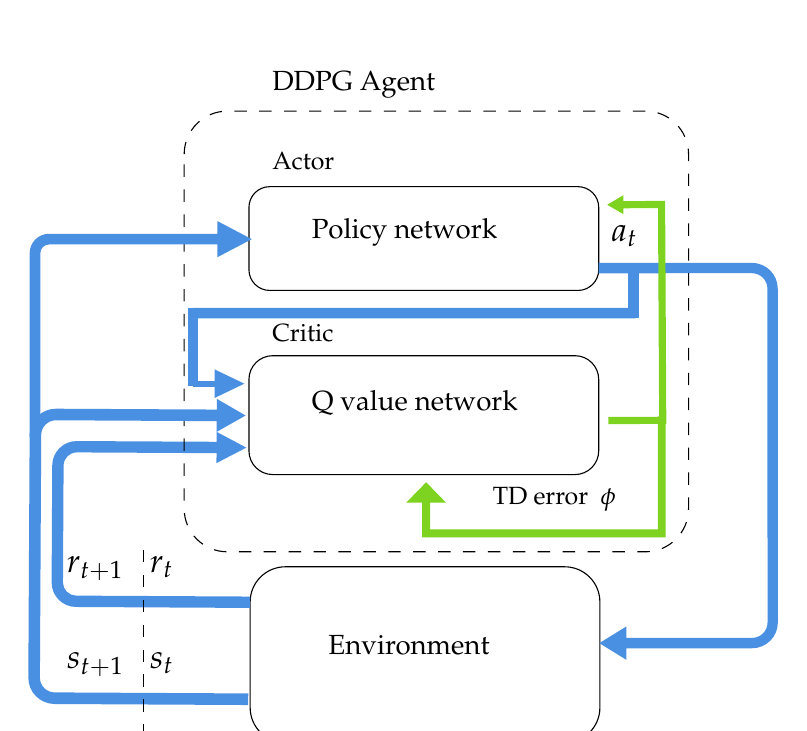
\begin{tikzpicture}[x=0.75pt,y=0.75pt,yscale=-1,xscale=1]
		%uncomment if require: \path (0,384); %set diagram left start at 0, and has height of 384
		
		%Rounded Rect [id:dp7665134511880258] 
		\draw   (253,93) .. controls (253,87.48) and (257.48,83) .. (263,83) -- (411.52,83) .. controls (417.04,83) and (421.52,87.48) .. (421.52,93) -- (421.52,123) .. controls (421.52,128.52) and (417.04,133) .. (411.52,133) -- (263,133) .. controls (257.48,133) and (253,128.52) .. (253,123) -- cycle ;
		%Rounded Rect [id:dp8334704830076491] 
		\draw   (253,175.89) .. controls (253,169.57) and (258.13,164.44) .. (264.46,164.44) -- (410.06,164.44) .. controls (416.39,164.44) and (421.52,169.57) .. (421.52,175.89) -- (421.52,210.26) .. controls (421.52,216.58) and (416.39,221.71) .. (410.06,221.71) -- (264.46,221.71) .. controls (258.13,221.71) and (253,216.58) .. (253,210.26) -- cycle ;
		%Rounded Rect [id:dp7924498191432374] 
		\draw   (253.58,283.1) .. controls (253.58,273.73) and (261.18,266.14) .. (270.54,266.14) -- (405.13,266.14) .. controls (414.49,266.14) and (422.08,273.73) .. (422.08,283.1) -- (422.08,333.97) .. controls (422.08,343.33) and (414.49,350.92) .. (405.13,350.92) -- (270.54,350.92) .. controls (261.18,350.92) and (253.58,343.33) .. (253.58,333.97) -- cycle ;
		%U Turn Arrow [id:dp5830248631009427] 
		\draw  [draw opacity=0][fill={rgb, 255:red, 74; green, 144; blue, 226 }  ,fill opacity=1 ] (421.53,119.74) -- (495.32,119.71) .. controls (502.2,119.71) and (507.78,125.29) .. (507.78,132.16) -- (507.83,292.94) .. controls (507.84,299.82) and (502.26,305.4) .. (495.39,305.4) -- (434.81,305.42) -- (434.81,310.94) -- (421.8,302.93) -- (434.81,294.92) -- (434.81,300.43) -- (495.38,300.41) .. controls (499.51,300.41) and (502.85,297.07) .. (502.85,292.94) -- (502.79,132.16) .. controls (502.79,128.04) and (499.45,124.7) .. (495.32,124.7) -- (421.53,124.73) -- cycle ;
		%U Turn Arrow [id:dp7331227116017869] 
		\draw  [draw opacity=0][fill={rgb, 255:red, 126; green, 211; blue, 33 }  ,fill opacity=1 ] (426.2,197.43) -- (453.9,197.28) .. controls (454.01,197.28) and (454.09,197.2) .. (454.09,197.09) -- (453.51,90.05) .. controls (453.51,89.94) and (453.43,89.86) .. (453.32,89.86) -- (433.36,89.96) -- (433.34,87.14) -- (425.63,91.73) -- (433.39,96.24) -- (433.38,93.42) -- (450.08,93.32) .. controls (450.08,93.32) and (450.08,93.32) .. (450.08,93.32) -- (450.62,193.85) .. controls (450.62,193.85) and (450.62,193.85) .. (450.62,193.85) -- (426.19,193.98) -- cycle ;
		%U Turn Arrow [id:dp9250538511454254] 
		\draw  [draw opacity=0][fill={rgb, 255:red, 126; green, 211; blue, 33 }  ,fill opacity=1 ] (453.8,193.85) -- (453.8,251.92) .. controls (453.8,251.92) and (453.8,251.92) .. (453.8,251.92) -- (336.47,251.92) .. controls (336.47,251.92) and (336.47,251.92) .. (336.47,251.92) -- (336.47,235.23) -- (328.8,235.23) -- (338.38,225.42) -- (347.96,235.23) -- (340.29,235.23) -- (340.29,248.1) .. controls (340.29,248.1) and (340.29,248.1) .. (340.29,248.1) -- (449.98,248.1) .. controls (449.98,248.1) and (449.98,248.1) .. (449.98,248.1) -- (449.98,193.85) -- cycle ;
		%U Turn Arrow [id:dp7567739250277439] 
		\draw  [draw opacity=0][fill={rgb, 255:red, 74; green, 144; blue, 226 }  ,fill opacity=1 ] (253.55,285.97) -- (169.68,285.51) .. controls (163.15,285.48) and (157.88,280.15) .. (157.92,273.62) -- (158.22,217.33) .. controls (158.26,210.79) and (163.58,205.52) .. (170.12,205.56) -- (237.41,205.92) -- (237.44,201.14) -- (251.73,208.74) -- (237.35,216.19) -- (237.38,211.41) -- (170.09,211.04) .. controls (166.58,211.02) and (163.72,213.85) .. (163.7,217.36) -- (163.4,273.65) .. controls (163.38,277.15) and (166.21,280.01) .. (169.71,280.03) -- (253.58,280.48) -- cycle ;
		%Rounded Rect [id:dp24819800426709504] 
		\draw  [dash pattern={on 4.5pt off 4.5pt}] (221.8,67.37) .. controls (221.8,55.9) and (231.1,46.6) .. (242.57,46.6) -- (444.03,46.6) .. controls (455.5,46.6) and (464.8,55.9) .. (464.8,67.37) -- (464.8,238.15) .. controls (464.8,249.63) and (455.5,258.92) .. (444.03,258.92) -- (242.57,258.92) .. controls (231.1,258.92) and (221.8,249.63) .. (221.8,238.15) -- cycle ;
		%U Turn Arrow [id:dp7033235171039725] 
		\draw  [draw opacity=0][fill={rgb, 255:red, 74; green, 144; blue, 226 }  ,fill opacity=1 ] (252.64,332.75) -- (159.32,332.25) .. controls (152.31,332.21) and (146.66,326.5) .. (146.7,319.49) -- (147.33,202.6) .. controls (147.37,195.59) and (153.08,189.94) .. (160.09,189.98) -- (237.49,190.39) -- (237.52,185.24) -- (251.39,193.26) -- (237.44,201.14) -- (237.46,195.98) -- (160.06,195.56) .. controls (156.14,195.54) and (152.94,198.7) .. (152.92,202.63) -- (152.29,319.52) .. controls (152.27,323.44) and (155.43,326.64) .. (159.35,326.66) -- (252.67,327.16) -- cycle ;
		%Bend Arrow [id:dp6257279516107521] 
		\draw  [draw opacity=0][fill={rgb, 255:red, 74; green, 144; blue, 226 }  ,fill opacity=1 ] (147.36,203.6) -- (147.36,115.02) .. controls (147.36,109.89) and (151.52,105.72) .. (156.66,105.72) -- (237.76,105.72) -- (237.76,99.57) -- (254.36,108.29) -- (237.76,117.01) -- (237.76,110.86) -- (156.66,110.86) .. controls (154.36,110.86) and (152.5,112.72) .. (152.5,115.02) -- (152.5,203.6) -- cycle ;
		%Straight Lines [id:da09269833954668538] 
		\draw  [dash pattern={on 4.5pt off 4.5pt}]  (202,348) -- (202,255.72) ;
		%Straight Lines [id:da4265551789273936] 
		\draw [color={rgb, 255:red, 74; green, 144; blue, 226 }  ,draw opacity=1 ][line width=3.75]    (439.3,143.92) -- (226,143.9) ;
		%Straight Lines [id:da03151350707279965] 
		\draw [color={rgb, 255:red, 74; green, 144; blue, 226 }  ,draw opacity=1 ][line width=3.75]    (226,179) -- (226,141.5) ;
		%Straight Lines [id:da8116483898702895] 
		\draw [color={rgb, 255:red, 74; green, 144; blue, 226 }  ,draw opacity=1 ][line width=3.75]    (438.3,146.2) -- (438.3,122.3) ;
		%Straight Lines [id:da1508384624951593] 
		\draw [color={rgb, 255:red, 74; green, 144; blue, 226 }  ,draw opacity=1 ][line width=2.25]    (245.8,177.92) -- (226,177.92) ;
		\draw [shift={(250.8,177.92)}, rotate = 180] [fill={rgb, 255:red, 74; green, 144; blue, 226 }  ,fill opacity=1 ][line width=0.08]  [draw opacity=0] (14.29,-6.86) -- (0,0) -- (14.29,6.86) -- cycle    ;
		
		% Text Node
		\draw (282,180) node [anchor=north west][inner sep=0.75pt]   [align=left] {Q value network};
		% Text Node
		\draw (282,97) node [anchor=north west][inner sep=0.75pt]   [align=left] {Policy network};
		% Text Node
		\draw (290,298) node [anchor=north west][inner sep=0.75pt]   [align=left] {Environment};
		% Text Node
		\draw (204,306) node [anchor=north west][inner sep=0.75pt]  [font=\large] [align=left] {$\displaystyle s_{t}$};
		% Text Node
		\draw (426.24,100.2) node [anchor=north west][inner sep=0.75pt]  [font=\large] [align=left] {$\displaystyle a_{t}$};
		% Text Node
		\draw (369.2,226.43) node [anchor=north west][inner sep=0.75pt]  [font=\small] [align=left] {TD error \ $\displaystyle \phi $};
		% Text Node
		\draw (263,65) node [anchor=north west][inner sep=0.75pt]  [font=\normalsize] [align=left] {{\small Actor}};
		% Text Node
		\draw (263,148) node [anchor=north west][inner sep=0.75pt]  [font=\small] [align=left] {Critic};
		% Text Node
		\draw (164,260) node [anchor=north west][inner sep=0.75pt]  [font=\large] [align=left] {$\displaystyle r_{t+1}$};
		% Text Node
		\draw (204,260) node [anchor=north west][inner sep=0.75pt]  [font=\large] [align=left] {$\displaystyle r_{t}$};
		% Text Node
		\draw (164,306) node [anchor=north west][inner sep=0.75pt]  [font=\large] [align=left] {$\displaystyle s_{t+1}$};
		% Text Node
		\draw (263,26) node [anchor=north west][inner sep=0.75pt]   [align=left] {DDPG Agent};
	\end{tikzpicture}
	\caption{Actor-Critic architecture: the actor produces an action given the current state of the environment, and the critic produces a temporal difference (TD) error signal given the state, the action, and the reward.}
	\label{fig:act_crit}
\end{figure}

To improve stability and efficiency, DDPG employs techniques like experience replay and target networks:
\begin{itemize}
	\item \textbf{Experience Replay:} The agent's experiences are stored in a replay buffer \( \mathcal{D} \), allowing the networks to be trained on random mini-batches of experiences. This breaks the temporal correlation between consecutive experiences and leads to more stable learning.
	\item \textbf{Target Networks:} Separate, slowly-updated target networks for both the actor and critic provide stable targets for the Q-value updates, reducing oscillations and divergence during training.
\end{itemize}

In summary, RL is a powerful framework for learning optimal policies through environmental interaction. The combination of RL with deep learning techniques like DDPG enables effective handling of complex, continuous action spaces, making it a versatile and robust approach for a wide range of applications.
When thinking about learning, one concept that immediately springs to mind is the notion of learning through interaction with the environment. This interaction provides us with insights into the effects of our actions, which can then be used to achieve goals. Reinforcement Learning (RL) is a machine learning technique that uses interactions to identify optimal behavior within an environment. In RL, the goal is to identify a policy—mapping states to actions—that maximizes the total expected reward. Rewards can accrue in both terminal and intermediate states. The agent seeks to gain valuable experience with states, actions, state transitions, and rewards to iteratively refine its behavior towards optimality. Unlike other machine learning paradigms, the evaluation of RL systems unfolds concurrently with the learning process. RL operates through a trial-and-error mechanism, navigating through delayed rewards while striking a balance between exploration and exploitation. More details on the DDPG algorithm can be found in \cite{DDPG}.

\end{appendices}



\backmatter


%La bibliografia è scritta utilizzando lo stile IEEE Transaction. I contenuti bibliografici, da poi richiamare nel testo, sono descritti nel file .bib
\normalem
\bibliographystyle{IEEEtran}
\bibliography{IEEEabrv,bib}

\end{document}